\documentclass[a4paper,10pt]{book}
\usepackage[utf8]{inputenc}
\usepackage[spanish]{babel}
\usepackage{physics}
\newcommand*\diff{\mathop{}\!\mathrm{d}}
\usepackage{fullpage}
\usepackage{cite}
\usepackage[utf8]{inputenc}
\usepackage{a4wide}
\usepackage{url}
\usepackage{graphicx}
\usepackage{caption}
\usepackage{float} % para que los gr\'aficos se queden en su lugar con [H]
\usepackage{subcaption}
\usepackage{wrapfig}
\usepackage{color}
\usepackage{amsmath} %para escribir funci\'on partida , matrices
\usepackage{amsthm} %para numerar definciones y teoremas
\usepackage[hidelinks]{hyperref} % para inlcuir links dentro del texto
\usepackage{tabu} 
\usepackage{comment}
\usepackage{amsfonts} % \mathbb{N} -> conjunto de los n\'umeros naturales  
\usepackage{enumerate}
\usepackage{listings}
\usepackage[colorinlistoftodos, textsize=small]{todonotes} % Para poner notas en el medio del texto!! No olvidar hacer. 
\usepackage{framed} % Para encuadrar texto. \begin{framed}
\usepackage{csquotes} % Para citar texto \begin{displayquote}
\usepackage{epigraph} % Epigrafe  \epigraph{texto}{\textit{autor}}
\usepackage{authblk}
\usepackage{titlesec}
\usepackage{varioref}
\usepackage{bm} % \bm{\alpha} bold greek symbol
\usepackage{pdfpages} % \includepdf
\usepackage[makeroom]{cancel} % \cancel{} \bcancel{} etc
\usepackage{wrapfig} % \begin{wrapfigure} Pone figura al lado del texto
\usepackage{mdframed}
\usepackage{algorithm}
%\usepackage{quoting}
\usepackage{mathtools}	
\usepackage{tikz}
\usepackage{paracol}
\usepackage[binary-units]{siunitx} % \num{} \SI{}
\usepackage{multirow}
% tikzlibrary.code.tex
%
% Copyright 2010-2011 by Laura Dietz
% Copyright 2012 by Jaakko Luttinen
%
% This file may be distributed and/or modified
%
% 1. under the LaTeX Project Public License and/or
% 2. under the GNU General Public License.
%
% See the files LICENSE_LPPL and LICENSE_GPL for more details.

% Load other libraries

%\newcommand{\vast}{\bBigg@{2.5}}
% newcommand{\Vast}{\bBigg@{14.5}}
% \usepackage{helvet}
% \renewcommand{\familydefault}{\sfdefault}

\usetikzlibrary{shapes}
\usetikzlibrary{fit}
\usetikzlibrary{chains}
\usetikzlibrary{arrows}

% Latent node
\tikzstyle{latent} = [circle,fill=white,draw=black,inner sep=1pt,
minimum size=20pt, font=\fontsize{10}{10}\selectfont, node distance=1]
% Observed node
\tikzstyle{obs} = [latent,fill=gray!25]
% Invisible node
\tikzstyle{invisible} = [latent,minimum size=0pt,color=white, opacity=0, node distance=0]
% Constant node
\tikzstyle{const} = [rectangle, inner sep=0pt, node distance=0.1]
%state
\tikzstyle{estado} = [latent,minimum size=8pt,node distance=0.4]
%action
\tikzstyle{accion} =[latent,circle,minimum size=5pt,fill=black,node distance=0.4]
\tikzstyle{fijo} =[latent,circle,minimum size=5pt,fill=black]


% Factor node
\tikzstyle{factor} = [rectangle, fill=black,minimum size=10pt, draw=black, inner
sep=0pt, node distance=1]
% Deterministic node
\tikzstyle{det} = [latent, rectangle]

% Plate node
\tikzstyle{plate} = [draw, rectangle, rounded corners, fit=#1]
% Invisible wrapper node
\tikzstyle{wrap} = [inner sep=0pt, fit=#1]
% Gate
\tikzstyle{gate} = [draw, rectangle, dashed, fit=#1]

% Caption node
\tikzstyle{caption} = [font=\footnotesize, node distance=0] %
\tikzstyle{plate caption} = [caption, node distance=0, inner sep=0pt,
below left=5pt and 0pt of #1.south east] %
\tikzstyle{factor caption} = [caption] %
\tikzstyle{every label} += [caption] %

\tikzset{>={triangle 45}}

%\pgfdeclarelayer{b}
%\pgfdeclarelayer{f}
%\pgfsetlayers{b,main,f}

% \factoredge [options] {inputs} {factors} {outputs}
\newcommand{\factoredge}[4][]{ %
  % Connect all nodes #2 to all nodes #4 via all factors #3.
  \foreach \f in {#3} { %
    \foreach \x in {#2} { %
      \path (\x) edge[-,#1] (\f) ; %
      %\draw[-,#1] (\x) edge[-] (\f) ; %
    } ;
    \foreach \y in {#4} { %
      \path (\f) edge[->,#1] (\y) ; %
      %\draw[->,#1] (\f) -- (\y) ; %
    } ;
  } ;
}

% \edge [options] {inputs} {outputs}
\newcommand{\edge}[3][]{ %
  % Connect all nodes #2 to all nodes #3.
  \foreach \x in {#2} { %
    \foreach \y in {#3} { %
      \path (\x) edge [->,#1] (\y) ;%
      %\draw[->,#1] (\x) -- (\y) ;%
    } ;
  } ;
}

% \factor [options] {name} {caption} {inputs} {outputs}
\newcommand{\factor}[5][]{ %
  % Draw the factor node. Use alias to allow empty names.
  \node[factor, label={[name=#2-caption]#3}, name=#2, #1,
  alias=#2-alias] {} ; %
  % Connect all inputs to outputs via this factor
  \factoredge {#4} {#2-alias} {#5} ; %
}

% \plate [options] {name} {fitlist} {caption}
\newcommand{\plate}[4][]{ %
  \node[wrap=#3] (#2-wrap) {}; %
  \node[plate caption=#2-wrap] (#2-caption) {#4}; %
  \node[plate=(#2-wrap)(#2-caption), #1] (#2) {}; %
}

% \gate [options] {name} {fitlist} {inputs}
\newcommand{\gate}[4][]{ %
  \node[gate=#3, name=#2, #1, alias=#2-alias] {}; %
  \foreach \x in {#4} { %
    \draw [-*,thick] (\x) -- (#2-alias); %
  } ;%
}

% \vgate {name} {fitlist-left} {caption-left} {fitlist-right}
% {caption-right} {inputs}
\newcommand{\vgate}[6]{ %
  % Wrap the left and right parts
  \node[wrap=#2] (#1-left) {}; %
  \node[wrap=#4] (#1-right) {}; %
  % Draw the gate
  \node[gate=(#1-left)(#1-right)] (#1) {}; %
  % Add captions
  \node[caption, below left=of #1.north ] (#1-left-caption)
  {#3}; %
  \node[caption, below right=of #1.north ] (#1-right-caption)
  {#5}; %
  % Draw middle separation
  \draw [-, dashed] (#1.north) -- (#1.south); %
  % Draw inputs
  \foreach \x in {#6} { %
    \draw [-*,thick] (\x) -- (#1); %
  } ;%
}

% \hgate {name} {fitlist-top} {caption-top} {fitlist-bottom}
% {caption-bottom} {inputs}
\newcommand{\hgate}[6]{ %
  % Wrap the left and right parts
  \node[wrap=#2] (#1-top) {}; %
  \node[wrap=#4] (#1-bottom) {}; %
  % Draw the gate
  \node[gate=(#1-top)(#1-bottom)] (#1) {}; %
  % Add captions
  \node[caption, above right=of #1.west ] (#1-top-caption)
  {#3}; %
  \node[caption, below right=of #1.west ] (#1-bottom-caption)
  {#5}; %
  % Draw middle separation
  \draw [-, dashed] (#1.west) -- (#1.east); %
  % Draw inputs
  \foreach \x in {#6} { %
    \draw [-*,thick] (\x) -- (#1); %
  } ;%
}



\tikzset{
every picture/.append style={
  execute at begin picture={\deactivatequoting},
  execute at end picture={\activatequoting}
  }
}

%%%%%% Para no numerar los prefacios, y todo lo que viene antes del capitulo 1. Coimenzar con \frontmatter y volver a abrir con \mainmatter
\makeatletter
\renewcommand{\frontmatter}{\cleardoublepage\@mainmatterfalse}
\renewcommand{\mainmatter}{\cleardoublepage\@mainmattertrue}
\makeatother
%%%%%%

\definecolor{julia}{rgb}{1, 0.5, 1}
\definecolor{python}{rgb}{1, 1, 0.5}
\definecolor{r}{rgb}{0.70, 0.80, 1}
\definecolor{all}{rgb}{0.85, 0.85, 0.85}


\usepackage{listings}
\lstset{
  aboveskip=3mm,
  belowskip=3mm,
  showstringspaces=true,
  columns=flexible,
  basicstyle={\footnotesize\ttfamily},
  breaklines=true,
  breakatwhitespace=true,
  tabsize=4,
  showlines=true
}

\hypersetup{
    colorlinks,
    linkcolor={black!50!black},
    citecolor={black!50!black},
    urlcolor={black!80!black}
}

\newcommand{\T}{Traducir. }
\newcommand{\vm}[1]{\mathbf{#1}}
\newcommand{\N}{\mathcal{N}}
\newcommand{\citel}[1]{\cite{#1}\label{#1}}
\newcommand\hfrac[2]{\genfrac{}{}{0pt}{}{#1}{#2}} %\frac{}{} sin la linea del medio

\newtheorem{midef}{Definition}
\newtheorem{miteo}{Theorem}
\newtheorem{mipropo}{Proposition}

\theoremstyle{definition}
\newtheorem{definition}{Definition}[section]
\newtheorem{theorem}{Theorem}[section]
\newtheorem{proposition}{Proposition}[section]

\newtheorem{conclution}{\en{Conclution}\es{Conclusi\'on}}%[section]
\newtheorem{objective}{\en{Objective}\es{Objetivo}}%[section]


%http://latexcolor.com/
\definecolor{azul}{rgb}{0.36, 0.54, 0.66}
\definecolor{rojo}{rgb}{0.7, 0.2, 0.116}
\definecolor{rojopiso}{rgb}{0.8, 0.25, 0.17}
\definecolor{verdeingles}{rgb}{0.12, 0.5, 0.17}
\definecolor{ubuntu}{rgb}{0.44, 0.16, 0.39}
\definecolor{debian}{rgb}{0.84, 0.04, 0.33}
\definecolor{dkgreen}{rgb}{0,0.6,0}
\definecolor{gray}{rgb}{0.5,0.5,0.5}
\definecolor{mauve}{rgb}{0.58,0,0.82}

\newif\ifen
\newif\ifes
\newcommand{\en}[1]{\ifen#1\fi}
\newcommand{\es}[1]{\ifes#1\fi}
\newcommand{\En}[1]{\ifen#1\fi}
\newcommand{\Es}[1]{\ifes#1\fi}

\estrue


\newcommand{\E}{\en{S}\es{E}}
\newcommand{\A}{\en{E}\es{A}}
\newcommand{\Ee}{\en{s}\es{e}}
\newcommand{\Aa}{\en{e}\es{a}}



% % % RENOMBRES
\newcommand{\TITULO}[0]{Análisis bayesiano del aprendizaje individual en comunidades de video juegos}
\newcommand{\TITULOen}[0]{Bayesian analysis of individual learning in video game communities}



%\title{\huge Creencias adaptativas, \\ cultura y aprendizaje social}
%%Inferencia bayesiana para el estudio del aprendizaje social en comunidades virtuales
\author{Gustavo Landfried}


\begin{document}

\deactivatequoting % Por incompatibilidad entre Babel spanish con > y < 

\frontmatter
\pagenumbering{roman}

\begin{center}

\includegraphics[scale=.8]{../logofcen.pdf}

\medskip
UNIVERSIDAD DE BUENOS AIRES

Facultad de Ciencias Exactas y Naturales

Departamento de Computaci\'on


\vspace{3cm}

\textbf{\LARGE \TITULO}
% \textsc{}

\vspace{1cm}



Tesis presentada para optar al t\'itulo de Doctor de la \\
Universidad de Buenos Aires en el \'area Ciencias de la Computaci\'on

\vspace{3cm}

\textbf{Lic. Gustavo Andr\'es Landfried}

\end{center}

\vspace{2.5cm}

\noindent Director de tesis: Dr. Esteban Mocskos 

\noindent Codirector de tesis: Dr. Diego Fern\'andez Slezak

\noindent Consejero de estudios: Dr. Hern\'an Melgratti \\

\noindent Lugar de trabajo: Departamento de Computaci\'on, Facultad de Ciencias Exactas y Naturales

\vspace{0.5cm}

\noindent Buenos Aires, Abril de 2022\\

\noindent Fecha de defensa: \\%13 de diciembre de 2018\\

\vspace{0.5cm}

\hspace*{0pt}\hfill Firma \hspace{2cm}

\newpage
%%%%%%%%%%%%% FIN CARATULA

\begin{center}
\Large \TITULO \normalsize
\end{center}

\hspace{2cm}

\begin{center}
\textbf{Resumen}
\end{center}

La cultura es un fen\'omeno poblacional que emerge como consecuencia del intercambio de informaci\'on entre individuos.
Esto sugiere que la estructura de la red de intercambios de informaci\'on afecta los procesos de evoluci\'on y acumulaci\'on cultural de los que dependen los individuos para el aprendizaje social.
Las hip\'otesis que han podido ser evaluadas confirman, por ejemplo, que la capacidad de acumulaci\'on cultural es proporcional al tamaño efectivo de la poblaci\'on, y que estructuras con moderada conexi\'on favorecen la evoluci\'on cultural.
Sin embargo, poner a prueba hip\'otesis más espec\'ificas se ha visto obstaculizado por la falta de modelos capaces de estimar correctamente las curvas de aprendizaje individuales y la falta de datos de comportamiento de todos los individuos de una comunidad en el tiempo.

Para explorar c\'omo la estructura de la red de intercambios afecta el aprendizaje individual, decidimos analizar las comunidades que se desarrollan alrededor de los videos juegos debido a que, además de permitirnos estudiar poblaciones suficientemente grandes con un alto grado de detalle, en ellas emergen y se desarrollan estrategias complejas de origen cultural.
En este contexto nos propusimos responder las siguientes preguntas.
¿C\'omo se puede medir el aprendizaje de un individuo en el tiempo?
¿Cu\'al es la relaci\'on entre la formaci\'on de equipos y el aprendizaje individual a largo plazo?
¿C\'omo tener en cuenta la estructura de la red de intercambios puede impactar en la mejora de la estimaci\'on de habilidad de las personas en el tiempo?
¿Cu\'al es el efecto que la posici\'on topol\'ogica de un individuo en la red de intercambios dinámica tiene sobre el aprendizaje individual?

A diferencia de las ciencias formales, las ciencias emp\'iricas deben validar sus proposiciones en sistemas abiertos que, por definici\'on, contienen siempre algún grado de incertidumbre.
¿Es posible alcanzar ``verdades'' si es inevitable decir `no sé''?
S\'i.
La aplicaci\'on estricta de las reglas de la probabilidad (enfoque bayesiano) garantiza los acuerdos inter-subjetivos en contextos de incertidumbre.
A pesar de que ha mostrado su potencialidad, su adopci\'on se vio hist\'oricamente limitada debido al alto costo computacional asociado a la evaluaci\'on de todo el espacio de hip\'otesis de acuerdo a los datos y los modelos causales.
Si bien en las últimas décadas estas limitaciones computacionales han sido superadas, en gran medida, debido al desarrollo de métodos eficientes de aproximaci\'on, la inercia hist\'orica sigue siendo una limitaci\'on importante.

Los estimadores de habilidad utilizados en la industria y la academia, por ejemplo, no aplican estrictamente las reglas de la probabilidad y, como consecuencia, no logran estimar correctamente las curvas de aprendizaje individuales en el tiempo.
Por este motivo, en esta tesis implementamos un modelo de estimaci\'on de habilidad (TrueSkill Through Time), que resuelve la inferencia apropiadamente, proporciona estimaciones con baja incertidumbre en todo la secuencia de eventos, permitiendo estimaciones iniciales de habilidad fiables y asegurando su comparabilidad hist\'orica.
Si bien la teor\'ia hab\'ia sido publicada hace más una década, nuestra implementaci\'on es la primera que la hace disponible en los lenguajes de programaci\'on con mayor desarrollo cient\'ifico como \texttt{Julia}, \texttt{Python} y \texttt{R}.
Los métodos de aproximaci\'on anal\'itica y los algoritmos de pasaje de mensajes permiten resolver la inferencia de forma eficiente utilizando aun cuando se cuente con bajos recursos de c\'omputo, incluso en redes causales con millones de nodos y estructuras irregulares.

A trav\'es de este modelo y de los datos de comunidades virtuales pudimos estudiar las preguntas planteadas.
En primer lugar pudimos observar, en una plataforma en el que las personas juegan individualmente o en equipos, que la tendencia a jugar en equipo estaba asociada una mejora de habilidad a largo plazo, y que quienes jugaban ``lealmente'' con una misma persona exhib\'ian un mayor velocidad en el la tasa de aprendizaje.
En segundo lugar pudimos evaluar, estudiando la dinámica de una red de intercambios de informaci\'on por un periodo de ocho años, que la posici\'on topol\'ogica de los individuos tiene un efecto de segundo orden y s\'olo en los jugadores que están en el medio del proceso de aprendizaje: los jugadores novatos aprenden principalmente por experiencia individual, y los jugadores expertos no tienen mucho más que aprender.

Durante el transcurso de esta tesis descubrimos el enorme potencial que la inferencia bayesiana y causal tiene para las ciencias sociales y las ciencias de datos en general, asimismo se desarrollaron una serie de paquetes para que esta herramienta pueda ser adoptada por la comunidad.

\vspace{0.3cm}

\noindent \textbf{Palabras claves}: Inferencia bayesiana, Evoluci\'on cultural, Conocimiento emp\'irico, Habilidad, Aprendizaje, Ciencias de la computaci\'on, Ciencias antropol\'ogicas, Epistemolog\'ia


\newpage

\begin{center}
\textbf{Abstract}
\end{center}


\vspace{0.3cm}

\noindent Keywords: Bayesian inference, Skill estimation, Learning, Computer science, Anthropological science, Computational social science 



\tableofcontents

\newpage 

\vfill

\pagenumbering{arabic}

\chapter{Agradecimientos}



\chapter{Prefacio}


\mainmatter




\chapter{Introducci\'on} \label{ch:evo}

% Parrafo: El objetivo subyacente de esta tesis. Interdisciplina entre la computación y las ciencias sociales.

Esta es una tesis, desde su concepción, ha tenido como objetivo subyacente sacar provecho del trabajo interdisciplinario entre las ciencias de la computación y las ciencias sociales.
%
Durante el transcurso del doctorado emergió con fuerza una sub disciplina, conocida como ciencias sociales computacionales~\ref{lazer2009-computationalSocialScience}, que tiene en la actualidad reconocimiento tanto en institutos de primer nivel de ciencias de la computación como en los gigantes tecnológicos relacionados a la industria del software.
%
Bajo esta categoría quedaron enmarcadas una gran variedad de actividades, a veces bastante diferentes entre si, desde aquellas que usan la computación como una herramienta para analizar datos de origen sociales, hasta aquellas que usan problemas de ciencias sociales para motivar desarrollos en la frontera del conocimiento en las ciencias de la computación~\ref{lazer2020-computationalSocialScience}.
%
Pero la emergencia de la interdiciplina es un fenómeno más general.
%
En la última década, impulsadas por los avances en el área de la inteligencia artificial, la masificación datos y métodos de aprendizaje automático, las ciencias de la computación ha tenido un impacto profundo en casi todas las disciplinas científicas, por no decir todas.
%
Una de sus consecuecias más contundentes quizás sea la emergencia e institucionalización de un área científica que ha nacido interdisciplinaria por definción: la ciencia de datos.

% Parrafo: interdisciplina sin datos (el ejemplo de la evolución cultural y la física)

Otras formas de interdisciplina sin datos, basada en modelos matemáticos, es posible y tiene una larga tradición entre las ciencias físicas y las ciencias sociales.
%
Si bien estos modelos son casi siempre demasiado simples para hacer predicciones, ayudan a entender procesos que son demasiado complejos para desentrañarse usando únicamente el lenguaje natural.
%
De la aplicación de la teoría de juegos al problema de la cooperación se desprendió uno de los cuerpos teóricos más influyentes para explicar como cambia la información cultural en el tiempo.
%
En la teorı́a de juegos evolucionaria \cite{taylor1978-replicatorDynamic, maynardSmith1982-evolutionGameTheory} es capaz de explicar equilibrios evolutivos que se producen entre estrategias en competencia cuando la adaptabilidad de ellas depende de las frecuencias de las otras posibles estrategias en la población.
%
Estos trabajos son, esencialmente, modelos formales teóricos que poseen poca o nula corroboración empı́rica, `pero que están destinados a comprender las consecuecias que ciertas relaciones causales podrían tener en fenómenos naturales en caso de que sus estructuras sean análogas.


% Parrafo: Datos y pregunta (evolución cultural / aprendizaje)

Para poner a prueba los métodos computacionales desarrolladas en el doctorado decidimos responder preguntas antropológicas sobre el aprendizaje social de los individuos en base de datos de comunidades de juegos en línea.


% Parrafo: Inferencia Bayesiana

Si bien el tema de la tesis está motivado por preguntas específicas acerca del del aprendizaje individual en comunidades de video juegos, esta tesis estuvo enfocada principalmente en los aspectos computacionales requeridos para hacer un correcto análisis de la evidencia empírica.
%
La ciencia es una institución humana que tiene pretención de verdad, esto es de formular proposiciones que valgan ``universalmente'' para todas las personas.
%
Las ciencias formales validan sus proposiciones mediante teoremas derivados de aplicar las reglas internas a un sistema axiomático cerrado.
%
Las ciencias empíricas, sin embargo, deben validar sus proposiciones dentro de sistemas abiertos que contienen siempre algún grado de incertidumbre.
%
Y el resultado, en términos profesionales y personales, ha sido mejor de lo esperado.
%
El razonamiento causal, basado en el enfoque bayesiano de la probabilidad, respondió las preguntas que tenía en antropología: cómo alcanzar acuerdos intersubjetivos en contextos de incertidumbre, fundamento de las verdades en todas las ciencias empíricas.
%
Para colmo resultó ser ideal para las ciencias sociales porque permite expresar los modelos causales mediante métodos gráficos intuitivos. Esto es más que una herramienta.





%Al inicio de la última revolución científica, entre mediados del 1600 y hasta mediados del 1800, la división de los problemas científicos en la ciencia se en disciplinaria

% La ciencia


\section{Evoluci\'on cultural}

La especial integraci\'on de los procesos biol\'ogicos, cognitivos y sociales que permiten a los humanos desarrollar culturas complejas se debi\'o a una coevoluci\'on gen\'etico-cultural desencadenada por el desarrollo previo de la crianza cooperativa~\cite{hrdy2020-emotionallyModern}.
%
La forma en la que estos homininos organizaron la crianza produjo un ambiente que favoreci\'o la selecci\'on de j\'ovenes capaces de monitorear y comprender las intenciones de los dem\'as, y de trasmitir a sus cuidadadores sus propias necesidades.
%A diferencia de nuestros parientes m\'as cercanos (chimpanc\'es, bonobos, gorilas y orangutanes)
Antes del surgimiento de los humanos anat\'omicamente modernos (masa cerebral actual) y de los humanos conductualmente modernos (lenguaje), surgi\'o en África una linaje emocionalmente moderno con capacidades para el entendimiento mutuo~\cite{hrdy2020-emotionallyModern}.

% Parrafo

La comprensi\'on mutua, la imitaci\'on y el lenguaje permitieron la transmisi\'on de conocimientos basados en la experiencia de otros (\emph{aprendizaje social}), dando inicio a un proceso cooperativo inter-generacional que produjo el desarrollo de la cultura, uns sistema de informaci\'on independiente al gen\'etico que permiti\'o a las poblaciones humanas adaptarse r\'apidamente a los cambiantes contextos ambientales.
%
El surgimiento de este nuevo sistema de informaci\'on produjo cambios radicales para nuestra especie.
%
Antes de la transici\'on cultural, estuvimos en grave peligro de extinci\'on, lo que se evidencia en la baja diversidad del genoma humano.
%
Luego de la transici\'on cultural, organizados en sociedades cazadores-recolectores, nuestra especie fue capaz de ocupar en pocos a\~nos todos los nichos ecol\'ogicos de la tierra como ning\'un otro vertebrado terrestre lo hab\'ia logrado antes.
%
Saliendo de África ocupamos Asia, Ocean\'ia y las Am\'ericas (Figura~\ref{fig:agricultura}).
% La informaci\'on transgeneracional fue la que le permiti\'o a estas sociedades simples adaptarse r\'apidamente a los nuevos desaf\'ios ecol\'ogicos.

\begin{figure}[ht!]
    \centering
    \begin{subfigure}[b]{0.6\textwidth}
     \includegraphics[width=\textwidth]{figures/agricultura.pdf}
     \label{fig:agricultura}
    \end{subfigure}
%     \begin{subfigure}[b]{0.40\textwidth}
%     \includegraphics[width=\textwidth]{static/polynesia.png} 
%     \caption{Poblamiento del oc\'eano Pac\'ifico}
%     \label{fig:polynesia}
%     \end{subfigure}
    \caption{
    Poblamiento humano (flechas) y surgimientos independientes de la agricultura (puntos).
    Proyecci\'on poli\'edrica de la tierra que conserva los tama\~nos relativos de los continentes.
    %Las felchas indican el poblamiento, desde África a Asia, y de Asia hacia Ocean\'ia y Am\'erica.
    %Los puntos rojos indican surgimiento independiente de agricultura.
    %El mapa de la figura~\ref{fig:polynesia}, desarrollado por Thorsby~\cite{thorsby2016-polynesiaAmerica}, muestra el poblamiento de la Polynesia y los contactos con Ámerica evidenciados en el material gen\'eticos.
    }%
    \label{fig:poblamiento}
\end{figure}

El cambio cultural es un fen\'omeno poblacional que emerge como consecuencia del intercambio de informaci\'on entre individuos.
%
Basada en los principios de la teor\'ia de la evoluci\'on (descendencia, modificaci\'on y selecci\'on), se ha desarrollado un marco te\'orico de \emph{evoluci\'on cultural} que intenta explicar c\'omo cambia la cultura en el tiempo.
%
La descendencia, mutaci\'on y selecci\'on de la informaci\'on cultural se produce cuando una persona adopta el comportamiento de otras, sea porque es el comportamiento de la mayor\'ia, sea porque la otra persona es particularmente exitosa o prestigiosa o por otros motivos.
%
Todos los procesos de aprendizaje social modifican en alg\'un grado la variante cultural adoptada.
%
Y algunas de esas variantes culturales se propagan m\'as r\'apido o son m\'as estables que otras, predominando en el tiempo.

% Parrafo

La experiencia acumulada a trav\'es de las generaciones por las m\'as diversas comunidades del mundo condujo, de forma independiente, al desarrollo de tecnolog\'ias de reciprocidad sorprendentemente similares entre s\'i.
%
La antropolog\'ia ha reconocido la existencia de una obligaci\'on universal de dar y de recibir.
%
La teor\'ia de la probabilidad nace en 1648 justamente como respuesta a la pregunta del \emph{precio justo} en contextos de incertidumbre.
%
El problema que analizaban Pascal y Fermat en sus cartas es equivalente al siguiente.
%
Tiramos dos veces la moneda.
%
Si sale Seca $S$ en la primera y en la segunda, una persona (en rojo) le hace un favor a la otra (en azul).
%
En caso contrario, el favor se invierte.
%
¿Cu\'al es el valor justo de la reciprocidad en este contexto de incertidumbre?

\begin{figure}[ht!]
    \centering
    \tikz{
    \node[latent, draw=white, yshift=0.7cm, minimum size=0.1cm] (b0) {};
    \node[latent,below=of b0,yshift=0.7cm, xshift=-1cm] (r1) {$S$};
    \node[latent,below=of b0,yshift=0.7cm, xshift=1cm] (r2) {$C$};

    \node[latent, below=of r1, draw=white, yshift=0.8cm, minimum size=0.1cm] (bc11) {};
    \node[accion, below=of r2, draw=white, yshift=0cm, color=blue!70] (bc12) {};
    \node[latent,below=of bc11,yshift=0.8cm, xshift=-0.5cm] (r1d2) {$S$};
    \node[latent,below=of bc11,yshift=0.8cm, xshift=0.5cm] (r1d3) {$C$};

    \node[accion,below=of r1d2,yshift=0cm, color=red!70] (br1d2) {};
    \node[accion,below=of r1d3,yshift=0cm, color=blue!70] (br1d3) {};
    \edge[-] {b0} {r1,r2};
    \edge[-] {r1} {bc11};
    \edge[-] {r2} {bc12};
    \edge[-] {bc11} {r1d2,r1d3};
    \edge[-] {r1d2} {br1d2};
    \edge[-] {r1d3} {br1d3};
    }
    \caption{El problema del \emph{valor justo} que da inicio a la teor\'ia de la probabilidad}
    \label{fig:pascal-fermat}
\end{figure}

La respuesta a la que arribaron Pascal y Fermat es que el valor de los favores tiene que ser inversamente proporcional a la probabilidad de hacer el favor.
%
En el caso de que la moneda sea no sesgada, hay 1/4 de probabilidad de que salgan dos Secas (terminal roja), 1/4 de que salga Seca en la primera y Cara en la segunda (terminal azul) y 1/2 de que salga Cara en la primera (terminal azul).
%
Luego, la probabilidad de que la persona azul haga un favor es 3/4.
%
Si la persona roja hace favores por un valor equivalente a 4, para que el intercambio se justo, la persona en azul tiene que devolver los favores por un valor de 4/3, una relaci\'on de 3 a 1.
%
Esta soluci\'on de calcular la probabilidad de un conjunto de eventos mutuamente excluyentes como suma de sus probabilidades elementales constituye el axioma fundamental de Kolmogorov a partir del cual se puede montar toda la teor\'ia de la probabilidad.

% Parrafo

Tanto los procesos de selecci\'on evolutiva como los probabil\'isticos son de naturaleza multiplicativa.
%
En la teor\'ia evolutiva todo el mundo aprende que el crecimiento de los linaje sigue un proceso multiplicativo y ruidoso: una productoria de las tasas de supervivencia y reproducci\'on.
%
Todas las axiomatizaciones alternativas de la teor\'ia de la probabilidad llegan a la conclusi\'on que las hip\'otesis se seleccionan mediante la regla del producto: la productoria de predicciones a priori de los datos observados.
%
Dado que en los procesos multiplicativos los impactos de las pérdidas suelen ser más fuertes que los de las ganancias (por ejemplo, un solo cero es suficiente para generar una extinci\'on) existe una ventaja a favor de aquellas variantes que reducen las fluctuaciones: diversificaci\'on individual (propiedad epistémica), cooperaci\'on (propiedad evolutiva mayor), especializaci\'on (propiedad meta-epistémica), coexistencia (propiedad ecol\'ogica)\footnote{La demostraci\'on de estas propiedades forman parte de un trabajo realizado durante del doctorado que no hemos incluido en esta tesis. }.

% Parrafo

La coexistencia con otras especies es la única estrategia posible para una especie heter\'otrofa como la nuestra.
%
Las tecnolog\'ias de reciprocidad ecol\'ogica produjeron la aparici\'on independiente de la domesticaci\'on de especies animales y vegetales, el desarrollo de caracteres gen\'eticos que surgen como resultado de una interacci\'on simbi\'otica prolongada entre las especies.
%
La agricultura surgi\'o de forma paralela en los seis grandes sistemas geogr\'aficos de la tierra (los puntos rojos de la figura~\ref{fig:agricultura}).
%
All\'i se desarrollaron los principales centros poblacionales de la humanidad.
%
El aumento de la poblaci\'on promovi\'o, a su vez, el desarrollo de nuevas innovaciones tecnol\'ogicas y cient\'ificas, como la escritura, la matem\'aticas, las ingenier\'ias, la astronom\'ia, las ciencias pol\'iticas, entre otras.
%
Durante el a\~no 1400 el mundo florec\'ia de sociedades ``pr\'osperas''~\cite{dussel2004-sistemaMundo}.
%
%El desarrollo tecnol\'ogico de todas estas sociedades fue extraordinario. 
%
% El imperio de Tonga ocupaba hace siglos todo el oc\'eano Pac\'ifico (figura~\ref{fig:polynesia}) con tecnolog\'ias de navegaci\'on que le hab\'ian permitido tener intercambios con Am\'erica de Sur~\cite{thorsby2016-polynesiaAmerica, ioannidis2020-polynesiaAmerica}.
% %
% En Am\'erica del Sur se hab\'ia desarrollado un sistema de intercambios basado en la reciprocidad de trabajo (minka, ayni y mita) que le permit\'ia a las comunidades administrar eficientemente el uso de los bienes comunes y al Estado desarrollar la infrastructura en el vasto territorio monta\~noso~\cite{murra1978-organizacion}.
% %
% En la regi\'on Azteca se hab\'ia desarrollado un extenso mercado regional con ciudades de hasta 300.000 habitantes, tres veces la ciudad de Venecia en esa misma \'epoca.%~\cite{www7.uc.cl}. %http://www7.uc.cl/sw_educ/historia/conquista/parte1/html/h54.html
% %
% El mundo \'Arabe comerciaba productos desde el Oc\'eano Pac\'ifico, en las Filipinas, hasta el Oc\'eano Atl\'antico, en Marruecos, conectando las innovaciones culturales de distintos hemisferios del planeta~\cite{dussel2004-sistemaMundo}.
% %
África siempre fue el continente m\'as diverso cultural y gen\'eticamente, pero quiz\'as el centro m\'as innovador en t\'erminos cient\'ificos y tecnolog\'ias haya sido la regi\'on de China~\cite{needham2004-generalConclusionsAndReflections}.

% Parrafo

John Needham, el brit\'anico que dedic\'o su vida a recopilar la monumental historia cient\'ifica y t\'ecnica de China, reconoce que comenz\'o a estudiar el tema motivado por responder la pregunta de por qu\'e s\'olo Europa occidental hab\'ia logrado el avance cient\'ifico.
%
\begin{quotation}
When I first formed the idea, about 1938, (...) I regarded the essential problem as that of why modern science had not developed in Chinese civilisation (or Indian or Islamic) but only in that of Europe~\cite{needham2004-generalConclusionsAndReflections}.%
\end{quotation}
Luego de 60 a\~nos de investigaciones, Needham se ve obligado inviertir la pregunta.
\begin{quotation}
Why, between the -1th century and the 15th century, was Chinese civilisation much \emph{more} efficient than occidental in gaining natural knowledge and in applying it to practical human needs?~\cite{needham2004-generalConclusionsAndReflections}
\end{quotation}

% Parrafo

Desde Hegel hasta la fecha, las explicaciones euroc\'entricas intentan explicar la prosperidad actual de occidente a trav\'es de una causa interna: la ``\'etica protestante'' de Max Weber~\cite{weber1905-eticaProtestante}, la ``mentalidad burguesa'' de Jos\'e Luis Romero~\cite{romero1967-revolucionBurguesa}, o m\'as recientemente el ``sistema de parentesco'' de Joseph Henrich~\cite{henrich2020-weirdest}.
%
La paradoja que no puede responder es c\'omo una sociedad sumida en un proceso de involuci\'on cultural \'unico, como la sociedad feudal de la ``edad media'', pudo generar de repente el extraordinario proceso de desarrollo cient\'ifico y t\'ecnico de la modernidad.

% Parrafo

As\'i como la integraci\'on favorece los proceso de innovaci\'on y acumulaci\'on cultural, el aislamiento está asociado a p\'erdidas masivas de informaci\'on cultural.
%
Un ejemplo paradigm\'atico de aislamiento total ocurre con la separaci\'on de Tasmania del continente Australiano por la subida del nivel del mar ocurrida a comienzos del Holonceno.
%
La evidencia indica que las sociedades que permanecieron en la isla de Tasmania perdieron gran parte de su cultura tecnol\'ogica.
%
La principal hip\'otesis sugiere que la reducci\'on del tama\~no efectivo de la poblaci\'on fue la causa de la p\'erdida cultural~\cite{Henrich2004}.
%
La capacidad de almacenamiento (e innovaci\'on) de tecnolog\'ias complejas requerir\'ia un tama\~no m\'inimo de la poblaci\'on, incluso en sociedades cazadoras-recolectoras.

% Parrafo

Un caso de aislamiento parcial ocurre en Europa occidental durante la Edad Media.
%
Antes de que tuviera lugar la Edad Media, el Imperio Romano produjo una p\'erdida masiva de diversidad cultural en su entorno, que tuvo consecuencias cr\'iticas para esta sociedad.
%
Arrinconada ya en el lejano occidente por el fr\'io polar al norte y la falta de tecnolog\'ias para navegar las aguas del oeste, Europa occidental comienza en el siglo octavo a quedar paulatinamente aislada del ``sistema mundo'' por la expansi\'on Árabe al sur y por la serie cismas con el Imperio Romano de Oriente~\cite{Dussel}.
%
Aislada parcialmente del sistema mundo, esta sociedad entra en un proceso de involuci\'on cultural que condujo a un deterioro extremo de las condiciones de vida.

% Parrafo

La pandemia que producen los migrantes feudales en América y el acceso a la enorme cantidad plata americana, moneda oficial de cambio en Eurasia, coloc\'o de repente a esta sociedad en una situaci\'on de integraci\'on privilegiada al sistema mundo. 
%
La plata de Am\'erica fluy\'o en todas las direcciones, principalmente en direcci\'on a China, iniciando un proceso r\'apido de acumulaci\'on cultural basado en las tecnolog\'ias extranjeras que impulsan la primera industrializaci\'on brit\'anica.
%
Más de dos siglos después del acceso a la plata Americana, Europa occidental segu\'ia consumiendo más productos asi\'aticos de los que pod\'ia exportar a Asia.
%
El comercio internacional de opio comenz\'o como respuesta a una crisis del comercio internacional europeo, especialmente brit\'anico.
%
El opio, un producto lujoso utilizado en China como medicina (raramente como estupefaciente), fue prohibida por los emperadores chinos en 1729 debido a que su abundancia hac\'ia crecer lentamente la cantidad de adictos~\cite{Kennet}.
%
Las consecuencias fueron m\'as graves cuando en 1818 se desarrolla una mezcla de opio m\'as barata y potente.

% Parrafo

Luego de la derrota de China contra el narco-estado brit\'anico, se establece por primera vez la hegemon\'ia de Europa occidental en el sistema mundo y comienza un proceso de colonizaci\'on en África continental, en los extensos territorios americanos que todav\'ia segu\'ian a manos de comunidades locales y el resto del mundo.
%
Comienza la era de los genocidios.
%
En todas las partes del globo, los exploradores y etn\'ografos fueron documentando la perdida de cultural debida al avance del frente colonial-moderno, estatal o privado, sobre las autonom\'ias locales.
%
Es una nueva era de avances cient\'ificos y tecnol\'ogicos, pero es el comienzo de la era de masiva p\'erdida de diversidad cultural.
%
La masiva p\'erdida de diversidad cultural trajo como consecuencia la masiva p\'erdida de biodiversidad actual.
%
A pesar de todos los avances cient\'ificos, la ciencia metropolitana moderna no fue capaz de compensar la p\'erdida de los conocimientos milenarios acumulados por las comunidades aut\'onomas locales.

% Parrafo

Los conocimientos culturales y cient\'ificos son recursos comunes justamente porque la reducci\'on de las fluctuaciones mediante la cooperaci\'on produjo un aumento de su tasa de crecimiento que provoc\'o la transici\'on cultural que nos permiti\'o salir del peligro de extinci\'on a ser capaces de ocupar todos los nichos ecol\'ogicos de la tierra organizados en simples sociedades cazadoras-recolectoras.
%
La integraci\'on privilegiada de la sociedad fedual al sistema mundo fue lo que le permiti\'o a esta sociedad, que estaba sumida en un proceso de involuci\'on cultural \'unico como el de la ``edad media'', generar de repente el extraordinario proceso de desarrollo cient\'ifico y t\'ecnico de la modernidad.
%
Sin embargo, la ruptura de la coexistencia intercultural que produce Europa a partir de mediados del siglo 19 habr\'ia causado una degradaci\'on irreparable en el recurso común cultural, a través de la pérdida de las tecnolog\'ias de reciprocidad ecol\'ogica locales, que nos conduce actualmente a una grave crisis de de pérdida masiva de diversidad cultural.

% Parrafo

Luego de la transici\'on cultural, cuando el conocimiento dej\'o de ser un recurso individual y pas\'o a ser un recurso cooperativo, dejamos de vernos obligados a reducir las fluctuaciones de forma individual y apareci\'o una ventaja a favor de la especializaci\'on: es mejor apostar todos por la mejor opci\'on aunque la mayor\'ia pueda fracasar individualmente.
%
Para incentivar la especializaci\'on y se vuelvan a desarrollar nuevas variantes culturales capaces de administrar exitosamente los intercambios con los sistemas ecol\'ogicos es necesario recuperar las autonom\'ias locales negadas todav\'ia hoy a las comunidades por los Estados modernos y el avance de agronegocio sobre sus territorios.
%
El proceso de evoluci\'on cultural necesariamente es cooperativo, y la coexistencia parece ser la \'unica estrategia posible, quienes la rompan sufran tarde o temprano las consecuencias.


\subsection{Objetivos} 

Con el objetivo de estudiar las consecuencias que los procesos multiplicativos de selecci\'on de variantes culturales tiene en un proceso natural, en esta tesis nos proponemos estudiar el efecto que algunos factores sociales tienen sobre el aprendizaje individual. 
%
Ya hemos señalado que la cultura es un fen\'omeno poblacional que emerge como consecuencia del intercambio de informaci\'on entre individuos.
%
Esto sugiere que el contexto social, la estabilidad o volatilidad de los v\'inculos, la estructura de la red de intercambios o el tama\~no de la poblaci\'on pueden afectar directa o indirectamente los procesos de aprendizaje social y acumulaci\'on cultural de los que dependen los individuos.
%
Poner a prueba estas hip\'otesis se ha visto obstaculizado por falta de datos granulares y longitudinales sobre el comportamiento de todos los individuos de una comunidad en el tiempo y de modelos capaces de ofrecer estimaciones de habilidad que permiten estimar correctamente las curvas de aprendizaje de las personas en el tiempo.

% Parrafo

La masificaci\'on del poder de c\'omputo y la posterior expansi\'on de Internet produjo una explosi\'on en la cantidad y calidad de datos generados por personas en todo el mundo.
%
Las comunidades virtuales ofrecen nuevos horizontes en la investigaci\'on cient\'ifica sobre comportamientos sociales pues re\'unen al mismo tiempo la posibilidad de estudiar poblaciones suficientemente grandes con un alto grado de detalle.
%
En esta tesis decidimos estudiar las comunidades que se desarrollan alrededor de los videos juegos, dado que esos escenarios tienen algunas las caracter\'isticas que las hacen especialmente interesantes para estudiar los problemas de aprendizaje.

% Parrafo

Conocer c\'omo las personas aprendemos es un problema importante para muchos \'ambitos de la vida, como la educaci\'on, el trabajo y el deporte.
%
En general las investigaciones se han enfocado principalmente en los factores cognitivos individuales del aprendizaje.
%
A pesar de que desde la antropolog\'ia se se\~nala la importancia que los factores sociales tienen sobre el aprendizaje, este enfoque no ha recibido la suficiente atenci\'on.
%
Por ello, en esta tesis decidimos estudiar algunas de las preguntas que permanecen abiertas.
%
¿C\'omo la formaci\'on de grupo afecta al aprendizaje?
%
¿Cu\'al es el efecto que la posici\'on en la red de intercambios tiene sobre el aprendizaje?

% Parrafo

\section{Teor\'ia de la probabilidad}\label{sec:principios_interculturales}

La coexistencia como fuente de validez del conocimiento nos obliga a rechazar la superioridad moral de subjetividades especiales o identidades particulares (criterio de autoridad) y a trabajar activamente para construir acuerdos inter-subjetivos que garanticen el principio de reconocimiento mutuo (criterio de coexistencia).
%
Elegimos el t\'ermino ``inter-subjetividad'', por sobre el de ``subjetividad'', debido a que el primero connota el cumplimiento de condiciones que son necesarias para producir el acuerdo entre las conciencias individuales, mientras que el segundo connota una arbitrariedad que lo obstaculiza.
%
Elegimos el t\'ermino ``intersubjetividad'', por sobre el de ``objetividad'', porque el primero connota una actividad constructiva entre los sujetos, mientras que el segundo connota la imposici\'on directa del objeto sobre los sujetos.

% Parrafo

% Para el proyecto intercultural de acuerdos intersubjetivos, que se propone la ciencia, se hace necesario que los individuos pongan en correspondencia un\'ivoca los fen\'omenos percibidos por sus conciencias con alg\'un esquema de operaci\'on que sea p\'ublicamente inteligible y reproducible.
% % 
% En este sentido, las funciones ocupan un rol fundamental.
% %
% En su definici\'on formal, una funci\'on es una relaci\'on (u operaci\'on) $f$ que a cada elemento de un conjunto (dominio) $X$ asigna un \'unico elemento de otro conjunto (imagen) $Y$.
% %
% \begin{equation}
%  \forall x \in X \  \exists! y \in Y \text{ tal que } f(x) = y    
% \end{equation}
% %
% %A primera vista puede parecer que las funciones no tienen nada en especial respecto de otro tipo de relaciones posibles entre conjuntos.
% Lo que hace tan poderosa a las funciones como herramienta para la ciencia es el hecho de que ellas permiten definir asignaciones no ambiguas.
% 
% % Parrafo
% 
% Los funciones son la base de las ciencias formales.
% %
% Todos los sistemas matem\'aticos de inter\'es est\'an compuestos por axiomas $X$, una serie de operaciones v\'alidas $F$, y un conjunto de consecuencias $Y$ consistentes entre s\'i.
% %
% En teor\'ia de la computabilidad, la tesis de Church-Turing afirma que toda funci\'on sobre los n\'umeros naturales puede ser calculada por un ``m\'etodo efectivo'' si y s\'olo si es computable por una m\'aquina de Turing.
% %
% Debido a que todos las definiciones alternativas del concepto  de ``m\'etodo efectivo'' resultaron ser equivalentes a una maquina de Turing, actualmente se supone que la hip\'otesis Church-Turing es cierta.
% 
% % Parrafo
% 
% Las funciones son tambi\'en la base de las ciencias emp\'iricas.
% %
% Veremos c\'omo los tres conceptos fundamentales de toda teor\'ia emp\'irica, los modelos causales, los datos y la incertidumbre tienen una estructura funcional.
% %
% En la secci\'on \ref{sec:principios_interculturales} introduciremos los principios interculturales de acuerdos intersubjetivos
% que garantizan los acuerdos intersubjetivos en contextos de incertidumbre.
% %
% En la secci\'on \ref{sec:reglas_de_la_probabilidad} presentaremos las reglas que se derivan del sistema de acuerdos intersubjetivos y explicaremos por qu\'e garantiza la adquisici\'on de conocimiento emp\'irico.
% %
% Uno de los principales problemas a resolver en ciencias emp\'iricas es la aparici\'on de modelos causales alternativos que compiten por la explicaci\'on de un mismo conjunto de observables.
% %
% En la secci\'on \ref{sec:modelos_alternativos} mostramos c\'omo las reglas de este sistema permiten realizar una selecci\'on intersubjetiva de modelos causales alternativos.
% %
% El otro problema fundamental en ciencias emp\'iricas es la constucci\'on de nuevos datos que sirvan como base emp\'irica para evaluar nuevas hip\'otesis.
% %
% En la secci\'on \ref{sec:base_empirica_metodo} d\'onde se ubican las hip\'otesis dentro de la estructura invariante del dato cient\'ifico, y c\'omo el sistema de acuerdos intersubjetivos garantiza la construcci\'on nueva base emp\'irica para la actividad cient\'ifica normal.
% 

A diferencia de las ciencias formales, que validan sus proposiciones mediante teoremas, resultados derivados de aplicar las reglas internas a un sistema axiomático cerrado, las ciencias emp\'iricas deben validar sus proposiciones dentro de sistemas abiertos, lo que impone siempre un grado de incertidumbre.
%
Las verdades emp\'iricas por lo tanto requieren que alcancemos acuerdos intersubjetivos, universales, en contextos de incertidumbre.
%
Un sistema l\'ogico con esas propiedades puede derivarse de principios filos\'oficos con validez intercultural.
%
En primer lugar, ``el principio de raz\'on suficiente'' es la base para el desarrollo de modelos causales.
%
El ``principio de integridad'' garantiza que no exista ni p\'erdida ni creaci\'on espontánea de creencias cuando la distribuimos entre las hip\'otesis alternativas.
%
El ``principio de indiferencia'' garantiza un primer acuerdo intersubjetivo en contextos de incertidumbre (máxima entrop\'ia dada informaci\'on disponible).
%
Finalmente, el ``principio de coherencia'' garantiza la continuidad del acuerdo intersubjetivo mediante la preservaci\'on de la creencia que que sigue siendo compatible con los datos de base emp\'irica.

\subsection{Principio de raz\'on suficiente}

La idea de que todo lo que ocurre en la naturaleza debe tener una causa previa que lo genere se conoce en la historia de la filosof\'ia como el principio de \emph{raz\'on suficiente}.
%
En pocas palabras, todo debe tener una explicaci\'on suficiente.
%Leibniz (1646-1716),  \cite{Leibniz and China: A Commerce of Light}
%La Monadolog\'ia (escrita en franc\'es en 1714 y publicada en alem\'an en 1720) es una de las obras de Gottfried Leibniz que mejor resume su filosof\'ia. Escrita hacia el final de su vida para sustentar una metaf\'isica de las sustancias simples, es un tratado acerca de las m\'onadas, que son los \'atomos verdaderos, es decir, realmente indivisibles. Se puede decir que es una proposici\'on filos\'ofica o metaf\'isica, aunque en ambos casos viene a significar lo mismo \cite{leibniz1714-monadologie}.
%
Este principio es la base del concepto de causa y efecto, que tiene nuevamente una estructura funcional, $f(x) = y$, donde $x$ representa las condiciones iniciales, $f$ el modelo causal determinista, e $y$ el efecto.

% Parrafo

Uno de los principales fundadores de la inferencia Bayesiana moderna, Pierre-Simon Laplace (1749-1827), ten\'ia la convicci\'on de que si tuviéramos conocimiento completo (infinitamente preciso) del estado del mundo $x$ en un instante de tiempo, y el modelo causal correcto que rige el comportamiento del mundo $f$, entonces tendr\'iamos conocimiento completo del estado del mundo en cualquier instante posterior $y$.
%
Aunque esta afirmaci\'on sea cierta (no existan eventos aleatorios en la naturaleza) conocer el mundo con precisi\'on \emph{finita} ha mostrado ser suficiente para introducir una incertidumbre que impide predecir el comportamiento de modelos causales, incluso en el corto plazo.
%
Un ejemplo de sistema determinista capaz de adquirir comportamientos imprevisibles es el siguiente modelo ``poblacional''.
%
\begin{equation}
 \text{Poblaci\'on}(t+1) = r \cdot \text{Poblaci\'on}(t)\cdot (1-\text{Poblaci\'on}(t))
\end{equation}
%
El modelo establece que el tama\~no de una poblaci\'on, medida como proporci\'on respecto de la capacidad m\'axima de un sistema, depende exclusivamente de su tama\~no en el tiempo anterior y de un factor de reproducci\'on $r$.
%
Las relaciones causales se suelen expresar en t\'erminos gr\'aficos.

% Parrafo

\begin{figure}[ht!]
\centering
\tikz{         
    \node[latent, minimum size=1.25cm] (n1) {$\text{pob}_n$} ; 
    
    \node[latent, right=of n1, xshift=3cm, minimum size=1.25cm] (n2) {$\text{pob}_{n+1}$} ;
    
     \path[->] (n1) edge node [yshift=0.5cm] {$r \cdot \text{pob}_n \cdot (1-\text{pob}_n)$} (n2);

}
\caption{Modelo causal expresado gr\'aficamente. Las flechas representan la relaci\'on causal entre las variables. }
\label{fig:modelo_poblacional}
\end{figure}

% Parrafo

Dependiendo del factor de reproducci\'on $r$ y de la poblaci\'on inicial pop$_0$, podemos observar diferentes tipos de comportamientos.
%
Por ejemplo, dada una poblaci\'on inicial $\text{pop}_0 = 0.5$, cuando el valor del par\'ametro $r$ es bajo (figura~\ref{fig:poblacion_punto_fijo}) la poblaci\'on tiende a un valor fijo;
cuando es intermedio (figura~\ref{fig:poblacion_periodico}) la poblaci\'on oscila en un per\'iodo;
y cuando llega a su l\'imite m\'aximo (figura~\ref{fig:poblacion_caotico}) la poblaci\'on tiene un comportamiento denominado ``ca\'otico''.
%
\begin{figure}[ht!]
    \centering
    \begin{subfigure}[b]{0.32\textwidth}
    \includegraphics[page=3,width=\linewidth]{figures/poblacion.pdf}
    \caption{Punto fijo}
    \label{fig:poblacion_punto_fijo}
    \end{subfigure}
    \begin{subfigure}[b]{0.32\textwidth}
    \includegraphics[page=9,width=\linewidth]{figures/poblacion.pdf}
    \caption{Peri\'odico}
    \label{fig:poblacion_periodico}
    \end{subfigure}
    \begin{subfigure}[b]{0.32\textwidth}
    \includegraphics[page=11,width=\linewidth]{figures/poblacion.pdf}
    \caption{Ca\'otico}
    \label{fig:poblacion_caotico}
    \end{subfigure}
    \caption{
    Tipos de atractores del modelo causal no-lineal
    }
    \label{fig:poblacion}
\end{figure}
%
Bajo un r\'egimen ca\'otico no se observan per\'iodos de ninguna longitud, el sistema produce trayectorias que nunca pasan por los mismos puntos.
%
En la figura \ref{fig:pseudo_aleatorio} vemos que los primeros 2000 puntos de la trayectoria determinista que comienza con $r=3.99$ y $\text{pop}_0 = 0.5$ se parece a una variable aleatoria.
%
Otra de las propiedades del atractor ca\'otico es la sensibilidad a las condiciones iniciales.
%
En la figura~\ref{fig:poblacion_caotico} hacemos zoom en los primeros 30 pasos temporales y observamos que si modificamos levemente las condiciones iniciales las trayectoria r\'apidamente divergen hasta volverse completamente diferentes.
%
\begin{figure}[ht!]
    \centering
    \begin{subfigure}[b]{0.4\textwidth}
    \centering
    \includegraphics[page=14,width=\linewidth]{figures/poblacion}
    \caption{Comportamiento que parece aleatorio}
    \label{fig:pseudo_aleatorio}
    \end{subfigure}
    \begin{subfigure}[b]{0.4\textwidth}
    \centering
    \includegraphics[page=13,width=\linewidth]{figures/poblacion}
    \caption{Sensibilidad a condiciones iniciales}
    \label{fig:sensibilidad}
    \end{subfigure}
    \caption{Comportamiento del modelo causal no lineal con $r=3.99$ y $\text{pop}_0 = 0.5$.
    (\subref{fig:pseudo_aleatorio}): primeros 2000 puntos.
    (\subref{fig:sensibilidad}): primeros 30 puntos. La linea roja comienza con $\text{pop}_0 = 0.499$.}
    \label{fig:propiedades_caoticas}
\end{figure}

%

La sensibilidad a las condiciones iniciales impone un l\'imite a la capacidad predictiva.
%
Por m\'as que la naturaleza sea determinista y conozcamos el mecanismo subyacente, si el sistema se encuentra bajo un atractor ca\'otico, jam\'as vamos a poder predecir el destino inevitable m\'as all\'a de cierto tiempo debido a que en ning\'un sistema natural podremos medir con infinita precisi\'on las condiciones iniciales.
%
La imposibilidad de determinar si estamos en presencia de \emph{exactamente} las mismas condiciones iniciales constituye ya una fuente de incertidumbre para las ciencias emp\'iricas.

\subsection{Principio de integridad}\label{sec:principio_integridad}

Las verdades emp\'iricas siempre contienen incertidumbre.
%
Hemos visto que un posible origen puede ser la sensibilidad a las condiciones iniciales de una naturaleza puramente causal.
%
Sin embargo, desde las ciencias sociales y la f\'isica cu\'antica se suele afirmar que el mundo no tiene forma de funci\'on: que incluso conociendo las condiciones iniciales con precisi\'on infinita no existe una funci\'on que permita determinar el estado del mundo en un tiempo posterior.

% Parrafo

El concepto de libre albedr\'io de las ciencias sociales afirma que una persona expuesta ante un estado del universo determinado, bajo exactamente las mismas condiciones iniciales, tiene todav\'ia la capacidad de elegir una acci\'on.
%
Ya no es posible definir una funci\'on tal que dado el estados inicial del universo $s$ devuelva la acci\'on $a$ que tomar\'a el sujeto, $f(s) = a$.
%
Sea porque el mundo natural admite la posibilidad de que un efecto surja sin su propia causa, sea por nuestra incapacidad de conocer los modelos causales correctos o de conocer las condiciones iniciales con infinita precisi\'on, nuestro conocimiento sobre el mundo natural contiene siempre un grado de incertidumbre.

% Parrafo

Supongamos que sabemos que las acciones sobre las que puede elegir la persona se limitan a esconder un regalo detr\'as de una caja entre tres.
%
Se abren as\'i tres ``universos paralelos'' posibles, uno por cada una de las acciones (figura~\ref{fig:libre_albedrio}).
%
\begin{figure}[ht!]
\centering
\begin{subfigure}[b]{0.48\textwidth}
\centering
    \scalebox{1}{
 \tikz{ %
        \node[estado] (s) {};
        \node[const, above=of s] {$s$};
        \node[accion, below=of s, xshift=-1cm] (a1) {} ; %
	\node[accion, below=of s, xshift=0cm] (a2) {} ; %
	\node[accion, below=of s, xshift=1cm] (a3) {} ; %
	\node[const, right=of a3] {$a$};
        \edge[-] {s} {a1,a2,a3};
      
	\node[estado, below=of a1,xshift=0cm] (s1a) {}; %
	  
	\node[estado, below=of a2,xshift=0cm] (s2a) {}; %
	   
	\node[estado, below=of a3,xshift=0cm] (s3a) {}; %
	    
	\node[const, right=of s3a] {$s^{\prime}$};
	\edge[-] {a1} {s1a};
	\edge[-] {a2} {s2a};
	\edge[-] {a3} {s3a};
        }
    
    }
    \caption{Libre albedr\'io}
    \label{fig:libre_albedrio}
\end{subfigure}
\begin{subfigure}[b]{0.48\textwidth}
 \centering
 \tikz{
    \node[factor, minimum size=0.8cm] (p1) {} ;
    \node[factor, minimum size=0.8cm, xshift=1.5cm] (p2) {} ;
    \node[factor, minimum size=0.8cm, xshift=3cm] (p3) {} ;
    
    \node[const, above=of p1, yshift=.15cm] (fp1) {$P(a_1)$};
    \node[const, above=of p2, yshift=.15cm] (fp2) {$P(a_2)$};
    \node[const, above=of p3, yshift=.15cm] (fp3) {$P(a_1)$};
    } 
   \caption{Espacio de hip\'otesis}
   \label{fig:espacio_de_hipotesis}
\end{subfigure}
    \caption{(a) El concepto te\'orico libre albedr\'io afirma que una persona, ante un estados $s$ del universo, es capaz de elegir entre m\'as de una acci\'on $a_i$.
    (b) Espacio de hip\'otesis: sabemos que hay un regalo detr\'as de s\'olo una de las tres cajas. }
\end{figure}
%
Cuando la incertidumbre nos impide conocer la funci\'on que gobierna el mundo, podemos todav\'ia expresar nuestra incertidumbre utilizando funciones de probabilidad, que para cada hip\'otesis $a$ asigne una proporci\'on $p$ de nuestra creencia total, $P(a_i) = p_i$.
%
En este caso, el conjunto de acciones posibles (esconder el regalo detr\'as de una de las tres cajas) representan nuestro \emph{espacio de hip\'otesis} (figura~\ref{fig:espacio_de_hipotesis}).
%
Y las diferentes formas de dividir la creencia le vamos a llamar \emph{distribuci\'on de creencias}.

% Parrafo

El ``principio de integridad'' establece la conservaci\'on de la creencia total, garantizando que no haya perdidas ni generaci\'on espont\'anea de creencias.
%
Esto es, que la suma de las proporciones asignadas a cada una de las hip\'otesis sea $1$.
%
\begin{equation}
\sum_{i} P(\text{hip\'otesis}_i) = 1
\end{equation}
%
Bajo este principio hay infinitas distribuciones de creencias posibles.
%
Por ejemplo, podemos tener el presentimiento de que est\'a en la caja del medio.
%
En la figura \ref{fig:distribucion_de_creencias} mostramos dos posibles distribuciones de creencias que tienen preferencia por esa caja.
%
La distribuci\'on de creencias de la figura~\ref{fig:preferencia_total} representa la certeza de que el regalo est\'a en la caja del medio, mientras que la figura~\ref{fig:preferencia_parcial} representa una preferencia parcial que mantiene todav\'ia cierta duda.

% PArrafo

\begin{figure}[ht!]     
 \centering
 \begin{subfigure}[b]{0.48\textwidth}
 \centering
  \tikz{ %
         \node[factor, minimum size=0.8cm] (p1) {} ;
         \node[factor, minimum size=0.8cm, xshift=1.5cm] (p2) {} ;
         \node[factor, minimum size=0.8cm, xshift=3cm] (p3) {} ;
         
         \node[const, above=of p1, yshift=.15cm] (fp1) {$0$};
         \node[const, above=of p2, yshift=.15cm] (fp2) {$1$};
         \node[const, above=of p3, yshift=.15cm] (fp3) {$0$};        
        }
    \caption{Preferencia total}
    \label{fig:preferencia_total}
 \end{subfigure}
 \begin{subfigure}[b]{0.48\textwidth}
 \centering
  \tikz{ %
         \node[factor, minimum size=0.8cm] (p1) {} ;
         \node[factor, minimum size=0.8cm, xshift=1.5cm] (p2) {} ;
         \node[factor, minimum size=0.8cm, xshift=3cm] (p3) {} ;
         
         \node[const, above=of p1, yshift=.15cm] (fp1) {$1/10$};
         \node[const, above=of p2, yshift=.15cm] (fp2) {$8/10$};
         \node[const, above=of p3, yshift=.15cm] (fp3) {$1/10$};        
        } 
    \caption{Preferencia parcial}
    \label{fig:preferencia_parcial}
 \end{subfigure}
\caption{Dos distribuci\'on de creencias que tienen preferencia por una de las hip\'otesis.}
 \label{fig:distribucion_de_creencias}
\end{figure}

% Parrafo

¿Pero cu\'al de todas las infinitas posibles distribuciones de creencias tiene validez intersubjetiva?

\subsection{Principio de indiferencia}\label{sec:principio_indiferencia}

El ``principio de indiferencia'' es un principio de validez intercultural que permite llegar a un primer acuerdo intersubjetivo en contextos de incertidumbre.
%
En los casos donde s\'olo conocemos el espacio de hip\'otesis y no tenemos m\'as informaci\'on que nos permita tener preferencia por ninguna de las opciones, vamos a estar de acuerdo en la necesidad de dividir la creencia en partes iguales por los caminos paralelos del modelo causal.
%
\begin{figure}[ht!]
\begin{subfigure}[b]{0.2\textwidth}
  \centering \vskip 0pt
  \tikz{            
    \node[latent] (r) {
\includegraphics[width=0.24\textwidth]{static/regalo.png}} ;
    \node[const,above=of r, yshift=.15cm] (nr) {$r \in \{1,2,3\}$} ; 
    \node[const, below=of r, yshift=-0.8cm] (title) {(a) Modelo causal};
   }
   
\end{subfigure}
\begin{subfigure}[b]{0.44\textwidth}
    \centering \vskip 0pt
    \tikz{
    \node[latent, draw=white, yshift=0.6cm] (b0) {$1$};
       
    \node[latent,below=of b0,yshift=0.6cm, xshift=-1.6cm] (r1) {$r_1$};
    \node[latent,below=of b0,yshift=0.6cm] (r2) {$r_2$};
    \node[latent,below=of b0,yshift=0.6cm, xshift=1.6cm] (r3) {$r_3$};

    \node[latent, below=of r1, draw=white, yshift=0.6cm] (br1) {$\frac{1}{3}$};
    \node[latent, below=of r2, draw=white, yshift=0.6cm] (br2) {$\frac{1}{3}$};
    \node[latent, below=of r3, draw=white, yshift=0.6cm] (br3) {$\frac{1}{3}$};
    \edge[-] {b0} {r1,r2,r3};
    \edge[-] {r1} {br1};
    \edge[-] {r2} {br2};
    \edge[-] {r3} {br3};
    
    \node[const, below=of br2, yshift=-0.1cm] (title) {(b) Caminos del modelo causal};
    }
\end{subfigure}
\begin{subfigure}[b]{0.32\textwidth}
\centering\vskip 0pt
\tikz{ %
        
         \node[factor, minimum size=1cm] (p1) {} ;
         \node[factor, minimum size=1cm, xshift=1.5cm] (p2) {} ;
         \node[factor, minimum size=1cm, xshift=3cm] (p3) {} ;
         \node[const, above=of p1, yshift=.15cm] (fp1) {$1/3$};
         \node[const, above=of p2, yshift=.15cm] (fp2) {$1/3$};
         \node[const, above=of p3, yshift=.15cm] (fp3) {$1/3$};
         \node[const, below=of p2, yshift=-0.8cm] (title) {(c) Creencia honesta};
         
        } 
\end{subfigure}
\caption{Principio de indiferencia. Figura (a): el modelo causal tiene una \'unica variable $r$ que puede tomar tres valores posibles. Figura (b): el modelo causal induce tres caminos paralelos por los que dividimos la creencia en partes iguales. Figura (c): como resultado obtenemos una creencia honesta que garantiza los acuerdos intersubjetivos dado el modelo causal.
}
\label{fig:principio_de_indiferencia}
\end{figure}
%
A este tipo de distribuciones de creencias que permiten alcanzar acuerdos intersubjetivos en contextos de incertidumbre las vamos a llamar \emph{creencia honestas}.

% Parrafo

El principio de indiferencia puede generalizarse a modelos causales multidimensional.
%
Para ejemplificar, supongamos que nos permiten elegir una caja $c$ y que despu\'es alguien nos se\~nala con certeza que el regalo no est\'a en la caja se\~nalada, $s$.
%
Es decir, tenemos tres variables y una dependencia causal, la pista $s$ depende de la posici\'on del regalo $r$.
%
¿Ser\'a que nuestra elecci\'on $c$ tambi\'en afecta la pista $s$?
%
Es decir, una opci\'on es que la pista solo dependa de la posici\'on del regalo, señale cualquier otra caja.
%
Otra opci\'on es que la pista adem\'as de no se\~nalar la caja donde est\'a el regalo, tampoco se\~nale la caja elegida.

% Parrafo

En este contexto podemos proponer al menos dos modelos causales multidimensionales alternativos.
%
En el primero hay s\'olo una dependencia causal, la pista no se\~nala la posici\'on del regalo, que podemos representar con el modelo causal de la figura~\ref{fig:modelo_causal_1}
%
En el segundo hay dos dependencias causales, la pista no se\~nala ni la posici\'on del regalo ni la caja elegida, que podemos representar con el modelo causal de la figura~\ref{fig:modelo_causal_2}.
%
Para simplificar el problema, consideraremos que la caja elegida es $c=1$.

% Parrafo

\begin{figure}[ht!]
  \centering
  \begin{subfigure}[b]{0.48\textwidth}
  \centering
  \tikz{            
    \node[latent,] (r) {
\includegraphics[width=0.12\textwidth]{static/regalo.png}} ;
    \node[const,left=of r] (nr) {\Large $r$} ;    
    
    
    \node[latent, below=of r] (d) {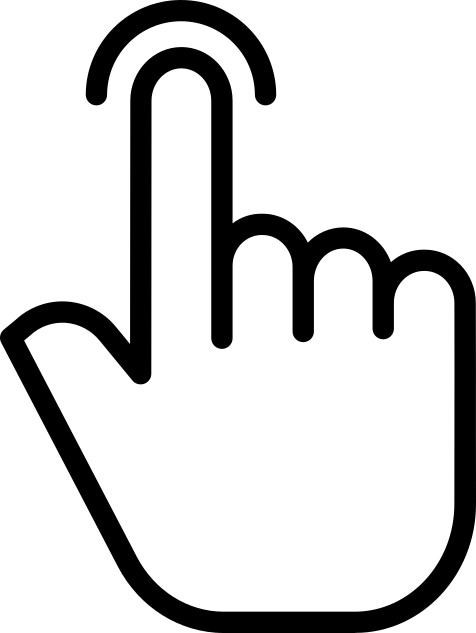
\includegraphics[width=0.10\textwidth]{static/dedo.png}} ;
    \node[const, left=of d] (nd) {\Large $s$};
    %\node[const, below=of d] (pd) {$\text{Creencia}(s=i|r=i, \text{Modelo}) = 0$}; 

    \edge {r} {d};
  }
  \caption{Modelo A}
  \label{fig:modelo_causal_1}
  \end{subfigure}
  \begin{subfigure}[b]{0.48\textwidth}
  \centering
  \tikz{        
    
    \node[latent] (d) {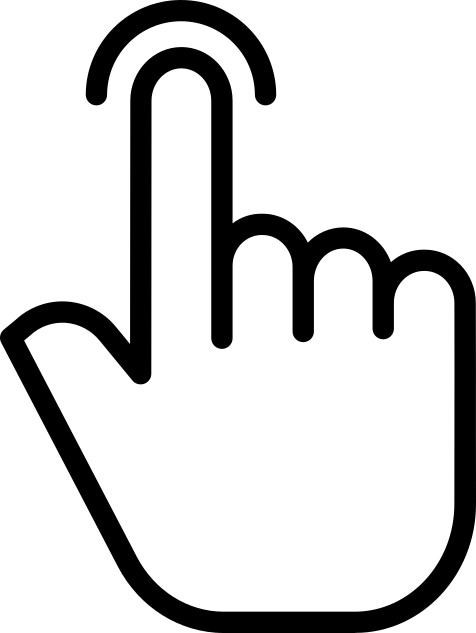
\includegraphics[width=0.10\textwidth]{static/dedo.png}} ;
    \node[const,above=of d] (nd) {\Large $s$} ;
    
    \node[latent, above=of d, xshift=-1.5cm] (r) {
\includegraphics[width=0.12\textwidth]{static/regalo.png}} ;
    \node[const,above=of r] (nr) {\Large $r$} ;
    
    \node[latent, fill=black!30, above=of d, xshift=1.5cm] (c) {
\includegraphics[width=0.12\textwidth]{static/cerradura.png}} ;
    \node[const,above=of c] (nc) {\Large $c=1$} ;
    
    \edge {r,c} {d};
  }
  \caption{Modelo B}
  \label{fig:modelo_causal_2}
  \end{subfigure}
  \caption{Modelos causales alternativos. Figura~\ref{fig:modelo_causal_1}: la pista s\'olo depende de la posici\'on del regalo. Figura~\ref{fig:modelo_causal_2}: la pista depende de la posici\'on del regalo y la la caja elegida previamente.
  Los c\'irculos representan las variables y la flecha representa la relaci\'on causa $\rightarrow$ efecto. 
  %A su vez, $r=i$ representa la proposici\'on ``el regalo se encuentra en la posici\'on $i$'', y $s=i$ representa la proposici\'on ``la pista se\~nala la posici\'on $i$''.
  }
  \label{fig:modelos_causales}
\end{figure}

% Parrafo
% %
% Por \'ultimo, lo que aparece del lado izquierdo del operador \emph{condicional} ($\cdot \mid \cdot$) son las proposiciones sobre las que computamos la creencia en los casos en los que las proposiciones que aparecen del lado derecha sean ciertas.
% %
% Es decir, la $\text{Creencia}(s=i|r=i,\text{Modelo}) = 0$ se lee como ``es imposible que la pista se\~nale la posici\'on $i$ cuando el regalo est\'a en la posici\'on $i$ y el modelo causal es cierto''. 
% 

% % Parrafo

Cada uno de los modelos causales alternativos tiene su propio conjunto finito de universos paralelos.
%
Siguiendo con el principio de indiferencia (o de m\'axima diversidad) dividimos la creencia en partes iguales en cada una de las bifurcaciones de los caminos paralelos del modelo causal.
%
En la figura~\ref{fig:caminos} mostramos c\'omo se dividen las creencias en partes iguales por los caminos paralelos de ambos modelos causales.

% Parrafo

En el modelo A, por cada posici\'on del regalo, se abren otros dos universos paralelos que se corresponden con las cajas hacia las que puede se\~nalar la pista, en las que no est\'a el regalo en ese universo.
%
En cambio, en el modelo B, la pista genera dos universos s\'olo cuando el regalo est\'a en la misma caja que elegimos, $r=c=1$.
%
% Podemos recibir una pista tanto en la puerta 2, $s_2$, como en la puerta 3, $s_3$.
% %
% Cuando el regalo est\'a en otra caja, $r\neq 1$, la pista puede se\~nalar \'unicamente a una de las cajas, la que no tiene el regalo y la que no fue elegida.
% %
% Por ejemplo, si el regalo est\'a en la puerta 2, $r_2$, la pista s\'olo puede se\~nalar la puerta 3, $s_3$.
%
\begin{figure}[H]
\centering
\begin{subfigure}[b]{0.48\textwidth}
\centering
\tikz{
\node[latent, draw=white, yshift=0.7cm] (b0) {$1$};

\node[latent,below=of b0,yshift=0.7cm, xshift=-2cm] (r1) {$r_1$};
\node[latent,below=of b0,yshift=0.7cm] (r2) {$r_2$};
\node[latent,below=of b0,yshift=0.7cm, xshift=2cm] (r3) {$r_3$};

\node[latent, below=of r1, draw=white, yshift=0.7cm] (br1) {$\frac{1}{3}$};
\node[latent, below=of r2, draw=white, yshift=0.7cm] (br2) {$\frac{1}{3}$};
\node[latent, below=of r3, draw=white, yshift=0.7cm] (br3) {$\frac{1}{3}$};
\node[latent,below=of br1,yshift=0.7cm, xshift=-0.5cm] (r1d2) {$s_2$};
\node[latent,below=of br1,yshift=0.7cm, xshift=0.5cm] (r1d3) {$s_3$};

\node[latent,below=of r1d2,yshift=0.7cm,draw=white] (br1d2) {$\frac{1}{3}\frac{1}{2}$};
\node[latent,below=of r1d3,yshift=0.7cm, draw=white] (br1d3) {$\frac{1}{3}\frac{1}{2}$};
\node[latent,below=of br2,yshift=0.7cm, xshift=-0.5cm] (r2d1) {$s_1$};
\node[latent,below=of br2,yshift=0.7cm, xshift=0.5cm] (r2d3) {$s_3$};
\node[latent,below=of br3,yshift=0.7cm, xshift=-0.5cm] (r3d1) {$s_1$};
\node[latent,below=of br3,yshift=0.7cm, xshift=0.5cm] (r3d2) {$s_2$};

\node[latent,below=of r2d1,yshift=0.7cm, draw=white] (br2d1) {$\frac{1}{3}\frac{1}{2}$};
\node[latent,below=of r2d3,yshift=0.7cm,draw=white] (br2d3) {$\frac{1}{3}\frac{1}{2}$};
\node[latent,below=of r3d1,yshift=0.7cm, draw=white] (br3d1) {$\frac{1}{3}\frac{1}{2}$};
\node[latent,below=of r3d2,yshift=0.7cm,draw=white] (br3d2) {$\frac{1}{3}\frac{1}{2}$};
\edge[-] {b0} {r1,r2,r3};
\edge[-] {r1} {br1};
\edge[-] {r2} {br2};
\edge[-] {r3} {br3};
\edge[-] {br1} {r1d2,r1d3};
\edge[-] {r1d2} {br1d2};
\edge[-] {r1d3} {br1d3};
\edge[-] {br2} {r2d1, r2d3};
\edge[-] {br3} {r3d1,r3d2};
\edge[-] {r2d1} {br2d1};
\edge[-] {r2d3} {br2d3};
\edge[-] {r3d1} {br3d1};
\edge[-] {r3d2} {br3d2};
}
\caption{Modelo A}
\label{fig:caminos_pre_montyhall}
\end{subfigure}
\begin{subfigure}[b]{0.48\textwidth}
\centering
\tikz{
\node[latent, draw=white, yshift=0.7cm] (b0) {$1$};
\node[latent,below=of b0,yshift=0.7cm, xshift=-2cm] (r1) {$r_1$};
\node[latent,below=of b0,yshift=0.7cm] (r2) {$r_2$};
\node[latent,below=of b0,yshift=0.7cm, xshift=2cm] (r3) {$r_3$};

% \node[latent, below=of r1, draw=white, yshift=0.8cm] (br1) {$\frac{1}{3}$};
% \node[latent, below=of r2, draw=white, yshift=0.8cm] (br2) {$\frac{1}{3}$};
% \node[latent, below=of r3, draw=white, yshift=0.8cm] (br3) {$\frac{1}{3}$};
% \node[latent,below=of br1,yshift=0.8cm] (c11) {$c_1$};
% \node[latent,below=of br2,yshift=0.8cm] (c12) {$c_1$};
% \node[latent,below=of br3,yshift=0.8cm] (c13) {$c_1$};

\node[latent, below=of r1, draw=white, yshift=0.7cm] (bc11) {$\frac{1}{3}$};
\node[latent, below=of r2, draw=white, yshift=0.7cm] (bc12) {$\frac{1}{3}$};
\node[latent, below=of r3, draw=white, yshift=0.7cm] (bc13) {$\frac{1}{3}$};
\node[latent,below=of bc11,yshift=0.7cm, xshift=-0.5cm] (r1d2) {$s_2$};
\node[latent,below=of bc11,yshift=0.7cm, xshift=0.5cm] (r1d3) {$s_3$};
\node[latent,below=of bc12,yshift=0.7cm] (r2d3) {$s_3$};
\node[latent,below=of bc13,yshift=0.7cm] (r3d2) {$s_2$};

\node[latent,below=of r1d2,yshift=0.7cm,draw=white] (br1d2) {$\frac{1}{3}\frac{1}{2}$};
\node[latent,below=of r1d3,yshift=0.7cm, draw=white] (br1d3) {$\frac{1}{3}\frac{1}{2}$};
\node[latent,below=of r2d3,yshift=0.7cm,draw=white] (br2d3) {$\frac{1}{3}$};
\node[latent,below=of r3d2,yshift=0.7cm,draw=white] (br3d2) {$\frac{1}{3}$};
\edge[-] {b0} {r1,r2,r3};
% \edge[-] {r1} {br1};
% \edge[-] {r2} {br2};
% \edge[-] {r3} {br3};
% \edge[-] {br1} {c11};
% \edge[-] {br2} {c12};
% \edge[-] {br3} {c13};
\edge[-] {r1} {bc11};
\edge[-] {r2} {bc12};
\edge[-] {r3} {bc13};
\edge[-] {bc11} {r1d2,r1d3};
\edge[-] {bc12} {r2d3};
\edge[-] {bc13} {r3d2};
\edge[-] {r1d2} {br1d2};
\edge[-] {r1d3} {br1d3};
\edge[-] {r2d3} {br2d3};
\edge[-] {r3d2} {br3d2};
}
\caption{Modelo B}
\label{fig:caminos_montyhall}
\end{subfigure}
\caption{Los caminos paralelos que se generan a partir de los modelos causales alternativos. El principio de m\'axima incertidumbre (o de indiferencia) divide la creencia en partes iguales en cada una de las bifurcaciones de los caminos paralelos del modelo causal. }
\label{fig:caminos}
\end{figure}
%
Esto nos permite definir creencias honestas respecto de los universos paralelos. 
%
El conjunto de creencias asignadas a los caminos paralelos del modelo causal representa nuestra \emph{creencia conjunta} honesta de que el regalo se encuentre en la caja $i$ y la pista se\~nale la caja $j$ (todas las posibles combinaciones de hip\'otesis).
%
\begin{table}[ht!]
\centering
$P(r=i, s=j | \text{Modelo A})$ \hspace{1.8cm} $P(r=i, s=j | \text{Modelo B})$ \\[0.1cm]
 \begin{tabular}{|c|c|c|c|} \hline \setlength\tabcolsep{0.4cm}
       & \, $r_1$ \, &  \, $r_2$ \, & \, $r_3$ \, \\ \hline 
  $s_1$ & $0$ & $1/6$ & $1/6$  \\ \hline
  $s_2$ & $1/6$ & $0$ & $1/6$  \\ \hline
  $s_3$ & $1/6$ & $1/6$ & $0$ \\ \hline 
  \end{tabular}
  \hspace{1.5cm}
  \begin{tabular}{|c|c|c|c|} \hline  \setlength\tabcolsep{0.4cm} 
 & \, $r_1$ \, &  \, $r_2$ \, & \, $r_3$ \,  \\ \hline 
  $s_1$ & $0$ & $0$ & $0$ \\ \hline
  $s_2$ & $1/6$ & $0$ & $1/3$ \\ \hline
  $s_3$ & $1/6$ & $1/3$ & $0$  \\ \hline  
  \end{tabular}
  \caption{Creencia conjunta para cada uno de los modelos causales. El valor de las celdas representa la creencia honesta sobre cada uno de los universos paralelos. }
  \label{tab:creencia_conjunta}
\end{table}
% Por ejemplo, la creencia conjunta de que el regalo est\'e en la caja $2$ y la pista se\~nale la caja $3$ es
% \begin{equation}
% \text{Creencia}(r=2 \wedge s=3 | \text{Modelo A} ) = \frac{1}{3} \frac{1}{2} = \frac{1}{6} \ \ \ \ \ \ \text{Creencia}(r=2 \wedge s=3 | \text{Modelo B} ) = \frac{1}{3} 
% \end{equation}
% %
% Donde $\wedge$ representa el conjunci\'on l\'ogica.
% %
% De aqu\'i en adelante remplazaremos este s\'imbolo por una simple coma ($,$).
% %
% Colocamos el modelo detr\'as del condicional ($\cdot|\cdot$) debido a que esta creencia conjunta es honesta cuando el modelo propuesto es cierto.
% %
% De aqu\'i en adelante s\'olo haremos expl\'icita la dependencia del modelo cuando haya alg\'un tipo de ambigüedad, que en general ocurre cuando hay m\'as de un modelo en disputa.
% %
% De la misma forma podemos calcular el resto de las creencias conjuntas a priori dado el modelo causal.
%
La conjunci\'on l\'ogica la expresamos con una simple coma ($,$), y colocamos del lado derecho del condicional ($\cdot|\cdot$) las proposiciones que momentáneamente consideramos ciertas.
%
Cada una de las celdas de la tabla representa una terminal de los caminos del modelo causal representados en la figura \ref{fig:caminos}.
%
Tenemos entonces un principio para alcanzar acuerdos sobre las creencias conjuntas cuando la \'unica informaci\'on previa es el modelo causal multidimensional.

% Parrafo

%Los caminos paralelos del modelo causal son hip\'otesis mutuamente excluytentes.
%
%Si ocurre uno de los caminos, no puede ocurrir el resto.
% 
% En ambos modelos, la pista se\~nala la caja $3$ cuando el regalo est\'a en la caja $1$ o en la caja $2$.
% Pero la creencia conjunta de esos caminos paralalelos es distinta.
% En el modelo A ambos caminos le asignamos una creencia de $1/6$, que sumadas representan $1/3$ de la creencia total.
% En el modelo B, en cambio, le asignamos una creencia de $1/6$ cuando el regalo est\'a en la caja $1$ y $1/3$ cuando el regalo est\'a en la caja $2$, que sumados represnetan $1/2$ del la creencia total.
% 
% % Parrafo
Habiendo definido la creencia conjunta sobre hip\'otesis mutuamente excluyentes (universos paralelos), por el principio de integridad podemos calcular la creencia correspondiente a cada una de las variables individuales mediante una suma.
%
\begin{equation}
\begin{split}
P(s_j|\text{Modelo A}) = \sum_i P(r_i, s_j|\text{Modelo A}) = 1/3 \\  P(s_j|\text{Modelo B}) = \sum_i P(r_i, s_j|\text{Modelo B}) = 1/2
\end{split}
\end{equation}

% Parrafo

Lo mismo ocurre con cualquiera de las variables de un modelo multidimensional.
%
Para calcular la creencia sobre una variable, calculamos la suma de todos los caminos paralelos en los que esa variable est\'a presente.

\begin{table}[H]
\centering
Modelo A  \hspace{4.5cm}  Modelo B \\[0.1cm]
 \begin{tabular}{|c|c|c|c||c|} \hline \setlength\tabcolsep{0.4cm}
       & \, $r_1$ \, &  \, $r_2$ \, & \, $r_3$ \, & \\ \hline 
  $s_1$ & $0$ & $1/6$ & $1/6$ & $1/3$ \\ \hline
  $s_2$ & $1/6$ & $0$ & $1/6$ & $1/3$ \\ \hline
  $s_3$ & $1/6$ & $1/6$ & $0$ & $1/3$ \\ \hline \hline
   & $1/3$ & $1/3$ & $1/3$ & $1$ \\ \hline 
  \end{tabular}
  \hspace{1.5cm}
  \begin{tabular}{|c|c|c|c||c|} \hline  \setlength\tabcolsep{0.4cm} 
 & \, $r_1$ \, &  \, $r_2$ \, & \, $r_3$ \, & \\ \hline 
  $s_1$ & $0$ & $0$ & $0$ & $0$\\ \hline
  $s_2$ & $1/6$ & $0$ & $1/3$ & $1/2$ \\ \hline
  $s_3$ & $1/6$ & $1/3$ & $0$ & $1/2$ \\ \hline \hline
   & $1/3$ & $1/3$ & $1/3$ & $1$  \\ \hline
  \end{tabular}
  \caption{Creencia marginal obtenida como la suma de las creencia conjuntas honesta de cada uno de los caminos paralelos de los modelos causales. }
  \label{tab:creencia_marginal}
\end{table}

En ambos modelos la creencia honesta sobre el regalos, sin importar el valor que toma pista, es $1/3$
%
\begin{figure}[H]
\centering
\tikz{ %
         \node[factor, minimum size=1cm] (p1) {
\includegraphics[width=0.025\textwidth]{static/cerradura.png}} ;
         \node[factor, minimum size=1cm, xshift=1.5cm] (p2) {} ;
         \node[factor, minimum size=1cm, xshift=3cm] (p3) {} ;

         \node[const, above=of p1, yshift=.15cm] (fp1) {$1/3$};
         \node[const, above=of p2, yshift=.15cm] (fp2) {$1/3$};
         \node[const, above=of p3, yshift=.15cm] (fp3) {$1/3$};
         \node[const, below=of p2, yshift=-.10cm, xshift=0.3cm] (dedo) {};
        } 
\caption{Creencia marginal sobre el regalo en ambos modelos causales. }
\end{figure}

\subsection{Principio de coherencia} \label{sec:principio_choerencia} % (dados los datos de base emp\'irica)

El principio de indiferencia nos permiti\'o definir la creencia conjunta honesta inicial, dividiendo las creencias en partes iguales por cada bifurcaci\'on del modelo causal.
%
Y el principio de integridad nos permiti\'o calcular la creencia honesta sobre una \'unica variable del modelo causal multidimensional, como la creencia total de todos los caminos paralelos en los que esa variable est\'a presente.
%
¿Pero c\'omo para preservar los acuerdos intersubjetivos cuando recibimos nueva informaci\'on?
%
El principio de coherencia establece que la nueva creencia honesta, despu\'es de haber visto un nuevo dato, es la creencia previa que sigue siendo compatible con ese dato.

% Parrafo

Supongamos que alguien nos indica con certeza que el regalo no est\'a en la caja del medio.
%
¿Cu\'al es la nueva creencia marginal honesta sobre el regalo despu\'es de haber visto esta pista?

% Parrafo

\begin{figure}[ht!]
\centering
\tikz{ %
        
         \node[factor, minimum size=1cm] (p1) {
\includegraphics[width=0.025\textwidth]{static/cerradura.png}} ;
         \node[det, minimum size=1cm, xshift=1.5cm] (p2) {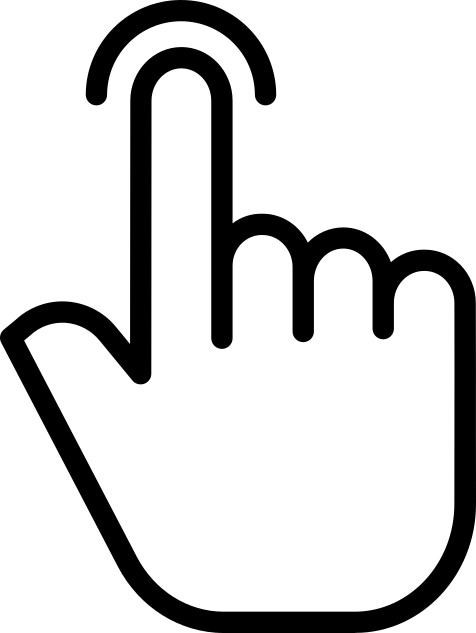
\includegraphics[width=0.03\textwidth]{static/dedo.png}} ;
         \node[factor, minimum size=1cm, xshift=3cm] (p3) {} ;
         \node[const, above=of p1, yshift=.15cm] (fp1) {$?$};
         \node[const, above=of p2, yshift=.15cm] (fp2) {$?$};
         \node[const, above=of p3, yshift=.15cm] (fp3) {$?$};
         \node[const, below=of p2, yshift=-.10cm, xshift=0.3cm] (dedo) {};
        
        } 
\end{figure}

% Parrafo

Para actualizar las creencias posiblemente nos veamos tentados a aplicar el principio de indiferencia nuevamente, asignando $0.5$ a las dos cajas restantes.
%
Aunque esa propuesta coincida con la soluci\'on correcta que obtendremos para el modelo A, esa 
decisi\'on conduce a errores en t\'erminos generales.
%
El principio de indiferencia s\'olo se aplica una \'unica vez, al inicio.
%
Despu\'es s\'olo actualizaremos esa creencia en funci\'on de la nueva informaci\'on que vayamos incorporando.

% Parrafo

Para actualizar las creencias simplemente nos quedamos con la creencia previa que es compatible con el dato.
%
Para ello nos quedamos con los caminos paralelos del modelo causal que siguen siendo compatible con el observable, $P(r_i, s_2)$.
%
\begin{table}[ht!]
\centering
$P(r=i, s=2 | \text{Modelo A})$ \hspace{2.7cm} $P(r=i, s=2 | \text{Modelo B})$ \\[0.1cm]
\begin{tabular}{|c|c|c|c||c|} \hline \setlength\tabcolsep{0.4cm}
       & \, $r_1$ \, &  \, $r_2$ \, & \, $r_3$ \, & \\ \hline 
  $s_2$ & $1/6$ & $0$ & $1/6$ & $1/3$ \\ \hline
  \end{tabular}
  \hspace{1.5cm}
  \begin{tabular}{|c|c|c|c||c|} \hline  \setlength\tabcolsep{0.4cm} 
 & \, $r_1$ \, &  \, $r_2$ \, & \, $r_3$ \, & \\ \hline 
  $s_2$ & $1/6$ & $0$ & $1/3$ & $1/2$ \\ \hline
  \end{tabular}
  \caption{La creencia conjunta y marginal que sobrevive luego de ver los datos. }
  \label{tab:creencia_compatible}
\end{table}

En la tabla~\ref{tab:creencia_compatible} nos quedamos con la creencia conjunta y marginal que sigue siendo compatible con el dato.
%
Esto es exactamente lo mismo que quedarnos con los caminos del modelo causal que son posibles dado el modelo causal y el observable.
%
En la figura~\ref{fig:caminos_compatibles} mostramos los caminos que son compatibles en negro y los incompatibles en gris.

\begin{figure}[ht!]
\centering
\begin{subfigure}[b]{0.48\textwidth}
\centering
\tikz{
\node[latent, draw=white, yshift=0.7cm] (b0) {$1$};

\node[latent,below=of b0,yshift=0.7cm, xshift=-2cm] (r1) {$r_1$};
{\color{gray}\node[latent,draw=gray,below=of b0,yshift=0.7cm] (r2) {$r_2$};}
\node[latent,below=of b0,yshift=0.7cm, xshift=2cm] (r3) {$r_3$};

\node[latent, below=of r1, draw=white, yshift=0.7cm] (br1) {$\frac{1}{3}$};
{\color{gray}\node[latent, below=of r2, draw=white, yshift=0.7cm] (br2) {$\frac{1}{3}$};}
\node[latent, below=of r3, draw=white, yshift=0.7cm] (br3) {$\frac{1}{3}$};
\node[latent,below=of br1,yshift=0.7cm, xshift=-0.5cm] (r1d2) {$s_2$};
{\color{gray}\node[latent,draw=gray,below=of br1,yshift=0.7cm, xshift=0.5cm] (r1d3) {$s_3$};}

\node[latent,below=of r1d2,yshift=0.7cm,draw=white] (br1d2) {$\frac{1}{3}\frac{1}{2}$};
{\color{gray} \node[latent,draw=gray,below=of r1d3,yshift=0.7cm, draw=white] (br1d3) {$\frac{1}{3}\frac{1}{2}$}; }
{\color{gray}\node[latent,draw=gray,below=of br2,yshift=0.7cm, xshift=-0.5cm] (r2d1) {$s_1$}; }
{\color{gray} \node[latent,draw=gray,below=of br2,yshift=0.7cm, xshift=0.5cm] (r2d3) {$s_3$}; }
{\color{gray} \node[latent,draw=gray,below=of br3,yshift=0.7cm, xshift=-0.5cm] (r3d1) {$s_1$}; }
\node[latent,below=of br3,yshift=0.7cm, xshift=0.5cm] (r3d2) {$s_2$};

{\color{gray}\node[latent,below=of r2d1,yshift=0.7cm, draw=white] (br2d1) {$\frac{1}{3}\frac{1}{2}$};}
{\color{gray}\node[latent,below=of r2d3,yshift=0.7cm,draw=white] (br2d3) {$\frac{1}{3}\frac{1}{2}$};}
{\color{gray}\node[latent,below=of r3d1,yshift=0.7cm, draw=white] (br3d1) {$\frac{1}{3}\frac{1}{2}$};}
\node[latent,below=of r3d2,yshift=0.7cm,draw=white] (br3d2) {$\frac{1}{3}\frac{1}{2}$};
\edge[-] {b0} {r1,r3};
\edge[-,draw=gray] {b0} {r2};
\edge[-] {r1} {br1};
\edge[-,draw=gray] {r2} {br2};
\edge[-] {r3} {br3};
\edge[-] {br1} {r1d2};
\edge[-,draw=gray] {br1} {r1d3};
\edge[-] {r1d2} {br1d2};
\edge[-,draw=gray] {r1d3} {br1d3};
\edge[-, draw=gray] {br2} {r2d1, r2d3};
\edge[-] {br3} {r3d2};
\edge[-, draw=gray] {br3} {r3d1};
\edge[-, draw=gray] {r2d1} {br2d1};
\edge[-, draw=gray] {r2d3} {br2d3};
\edge[-, draw=gray] {r3d1} {br3d1};
\edge[-] {r3d2} {br3d2};
}
\caption{Modelo A}
\label{fig:caminos_pre_montyhall_compatibles}
\end{subfigure}
\begin{subfigure}[b]{0.48\textwidth}
\centering
\tikz{
\node[latent, draw=white, yshift=0.7cm] (b0) {$1$};
\node[latent,below=of b0,yshift=0.7cm, xshift=-2cm] (r1) {$r_1$};
{\color{gray}\node[latent,draw=gray,below=of b0,yshift=0.7cm] (r2) {$r_2$}; }
\node[latent,below=of b0,yshift=0.7cm, xshift=2cm] (r3) {$r_3$}; 

% \node[latent, below=of r1, draw=white, yshift=0.8cm] (br1) {$\frac{1}{3}$};
% \node[latent, below=of r2, draw=white, yshift=0.8cm] (br2) {$\frac{1}{3}$};
% \node[latent, below=of r3, draw=white, yshift=0.8cm] (br3) {$\frac{1}{3}$};
% \node[latent,below=of br1,yshift=0.8cm] (c11) {$c_1$};
% \node[latent,below=of br2,yshift=0.8cm] (c12) {$c_1$};
% \node[latent,below=of br3,yshift=0.8cm] (c13) {$c_1$};

\node[latent, below=of r1, draw=white, yshift=0.7cm] (bc11) {$\frac{1}{3}$};
{\color{gray}\node[latent, below=of r2, draw=white, yshift=0.7cm] (bc12) {$\frac{1}{3}$};}
\node[latent, below=of r3, draw=white, yshift=0.7cm] (bc13) {$\frac{1}{3}$};
\node[latent,below=of bc11,yshift=0.7cm, xshift=-0.5cm] (r1d2) {$s_2$};
{\color{gray}\node[latent,draw=gray,below=of bc11,yshift=0.7cm, xshift=0.5cm] (r1d3) {$s_3$};}
{\color{gray}\node[latent, draw=gray,below=of bc12,yshift=0.7cm] (r2d3) {$s_3$};}
\node[latent,below=of bc13,yshift=0.7cm] (r3d2) {$s_2$};

\node[latent,below=of r1d2,yshift=0.7cm,draw=white] (br1d2) {$\frac{1}{3}\frac{1}{2}$};
{\color{gray}\node[latent,below=of r1d3,yshift=0.7cm, draw=white] (br1d3) {$\frac{1}{3}\frac{1}{2}$};}
{\color{gray}\node[latent,below=of r2d3,yshift=0.7cm,draw=white] (br2d3) {$\frac{1}{3}$};}
\node[latent,below=of r3d2,yshift=0.7cm,draw=white] (br3d2) {$\frac{1}{3}$};
\edge[-] {b0} {r1,r3};
\edge[-,draw=gray] {b0} {r2};
% \edge[-] {r1} {br1};
% \edge[-] {r2} {br2};
% \edge[-] {r3} {br3};
% \edge[-] {br1} {c11};
% \edge[-] {br2} {c12};
% \edge[-] {br3} {c13};
\edge[-] {r1} {bc11};
\edge[-,draw=gray] {r2} {bc12};
\edge[-] {r3} {bc13};
\edge[-] {bc11} {r1d2};
\edge[-,draw=gray] {bc11} {r1d3};
\edge[-,draw=gray] {bc12} {r2d3};
\edge[-] {bc13} {r3d2};
\edge[-] {r1d2} {br1d2};
\edge[-,draw=gray] {r1d3} {br1d3};
\edge[-,draw=gray] {r2d3} {br2d3};
\edge[-] {r3d2} {br3d2};
}
\caption{Modelo B}
\label{fig:caminos_montyhall_compatibles}
\end{subfigure}
\caption{Los caminos paralelos compatibles (negro) e incompatibles (gris) con el dato $s=2$. }
\label{fig:caminos_compatibles}
\end{figure}
% Cuando aplicamos por primera vez el principio de indiferencia en la figura \ref{fig:principio_de_indiferencia}, el espacio de hip\'otesis se reduc\'ia a tres opciones, una por caja.
% %
% En este caso, en el que estamos considerando una variable nueva (la se\~nal $s$) que representa la pista, el espacio de hip\'otesis es otro, m\'as grande, por lo que esta creencia a priori no nos sirve.
% %

Es decir, para actualizar nuestra creencia nos quedamos con la creencia a priori que es compatible con los datos.
%
Lo que nos permitir\'a cumplir el objetivo que nos hab\'iamos propuesto, actualizar la creencia sobre el regalo luego de haber visto la pista.
%
\textbf{La creencia que sobrevive}, $P(r_i, s_2)$, es ahora nuestra nueva creencia total.
%
Para expresarla nuevamente como tal, la normalizamos para que vuelva a sumar 1.
%
\begin{equation}
P(r_i| s_2, \text{Modelo} ) = \frac{P(r_i, s_2| \text{Modelo})}{P(s_2| \text{Modelo})}
\end{equation}
%
La concusi\'on a la que llegamos depende del modelo causal elegido.
\begin{figure}[ht!]
\centering
\begin{subfigure}[b]{0.48\textwidth}
\centering
\tikz{ %
        
         \node[factor, minimum size=1cm] (p1) {
\includegraphics[width=0.05\textwidth]{static/cerradura.png}} ;
         \node[det, minimum size=1cm, xshift=1.5cm] (p2) {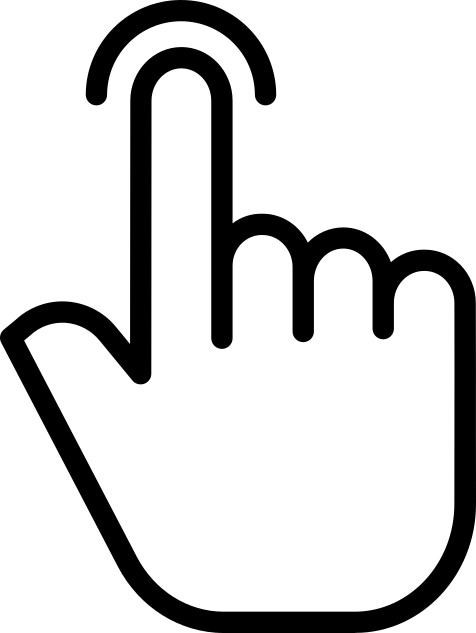
\includegraphics[width=0.06\textwidth]{static/dedo.png}} ;
         \node[factor, minimum size=1cm, xshift=3cm] (p3) {} ;

         \node[const, above=of p1, yshift=.15cm] (fp1) {$1/2$};
         \node[const, above=of p2, yshift=.15cm] (fp2) {$0$};
         \node[const, above=of p3, yshift=.15cm] (fp3) {$1/2$};
         \node[const, below=of p2, yshift=-.10cm, xshift=0.3cm] (dedo) {};
}
\caption{Modelos A}
\end{subfigure}
\begin{subfigure}[b]{0.48\textwidth}
\centering
\tikz{ %
        
         \node[factor, minimum size=1cm] (p1) {
\includegraphics[width=0.05\textwidth]{static/cerradura.png}} ;
         \node[det, minimum size=1cm, xshift=1.5cm] (p2) {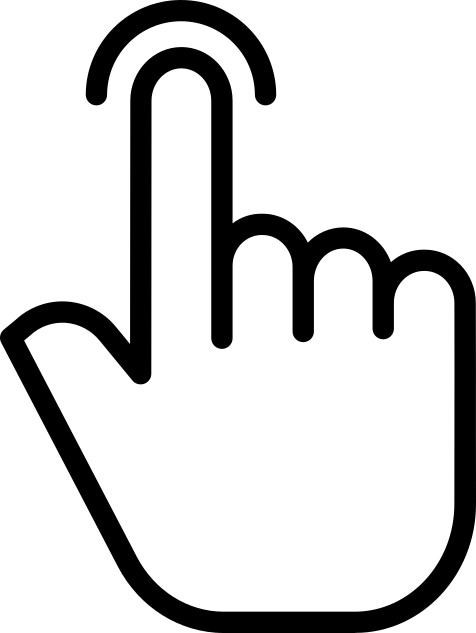
\includegraphics[width=0.06\textwidth]{static/dedo.png}} ;
         \node[factor, minimum size=1cm, xshift=3cm] (p3) {} ;
         
         \node[const, above=of p1, yshift=.15cm] (fp1) {$1/3$};
         \node[const, above=of p2, yshift=.15cm] (fp2) {$0$};
         \node[const, above=of p3, yshift=.15cm] (fp3) {$2/3$};
         \node[const, below=of p2, yshift=-.10cm, xshift=0.3cm] (dedo) {};
        }
\caption{Modelo B}
\end{subfigure}
\caption{Nueva creencia honesta dada el dato y el modelo}
\end{figure}
%  
Si bien ambas respuesta son diferentes, ambas comparten la propiedad de ser la distribuci\'on de creencias que maximiza la incertidumbre dada la evidencia formal (modelo causal) y emp\'irica (datos), el acuerdo intersubjetivo si el modelo causal y los datos fueran ciertos.

\section{Las reglas de la probabilidad}\label{sec:reglas_de_la_probabilidad}

La teor\'ia de la probabilidad es actualmente el enfoque más utilizado para representar incertidumbre asociada al conocimiento emp\'irico.
%
La teor\'ia de la probabilidad puede resumirse en dos reglas, conocidas como la regla de la suma y la regla del producto.
%
La regla de la suma proviene del principio de integridad y establece que cualquier creencia marginal puede ser obtenida integrando la creencia conjunta.
%
\begin{equation}
P(r_i) = \sum_j P(r_i, s_j)
\end{equation}
%
La segunda regla proviene del principio de coherencia y, expresada como producto, establece que cualquier distribuci\'on conjunta puede ser expresada como el producto de distribuciones condicionales uni-dimensionales.
%
\begin{equation}
P(s_j)P(r_i|s_j) = P(r_i, s_j)
\end{equation}

% Parrafo

Las reglas de la probabilidad han sido derivadas formalmente a partir de varios sistemas axiom\'aticos conceptualmente distintos e independientes entre si, lo cual es uno de los puntos fuertes a su favor~\cite{halpern2017}.
%
El sistema axiom\'atico de Cox~\cite{cox} las deriva a partir de axiomas del ``sentido común''.
%
El sistema axiom\'atico de Ramsey~\cite{ramsey} las deriva haciendo una analog\'ia con los pagos que aceptar\'iamos en una apuesta. 
%
El sistema axiom\'atico de Kolmogorv~\cite{kolmogorov} tiene una motivaci\'on filos\'ofica menos expl\'icita, pero su simplicidad matem\'atica hace que sea el sistema de referencia.
%
En el sistema de Kolmogorov la regla de la suma forma parte de los axiomas y la regla del producto de una definici\'on complementaria.
%
\begin{quotation}
Sea $E$ un conjunto de elementos $e_1, e_2, \dots$, y $F$ conjunto de subconjuntos de $E$.
%
\begin{enumerate}\itemsep-0.05cm
\item $F$ est\'a cerrada bajo complementos, uniones e intersecciones contables.
\item $F$ contiene al conjunto $E$
\item Todo conjunto $S \in F$ se le asigna una n\'umero real no negativo, $P(S)$.
\item $P(E) = 1$
\item Si $S_1, S_2, \dots$ son conjuntos mutuamente excluyente, luego
\begin{equation}
P(S_1 \cup S_2 \cup \dots ) = \sum P(S_i)
\end{equation}
\end{enumerate}
\end{quotation}
%
La regla de la suma se deriva inmediatamente del axioma 5 dado que siempre podemos expresar cualquier conjunto como $A = A \cap (B \cup \neg B)$.
%
La probabilidad condicional (o regla del producto) se incluye en el sistema como una definici\'on que cumple con los axiomas de la probabilidad. 

% %Ciertamentese ha dedicado mucho m\'as esfuerzo a justificar la teor\'ia de la probabilidad que cualquier otro enfoque para representar la incertidumbre y el tiempo dir\'a si se pueden se pueden desarrollar otros enfoques superadores.
% Pero quiz\'as m\'as importante es que su aplicaci\'on estricta (lo que llamamos inferencia Bayesiana) garantiza los acuerdos intersubjetivos a trav\'es de la maximizaci\'on de la incertidumbre (entrop\'ia) dada la informaci\'on emp\'irica y formal (datos y modelos causales)~\cite{Jaynes2003}.
% %

% Parrafo

As\'i expresada, la teor\'ia de la probabilidad est\'a basada en s\'olo dos de los cuatro principios vistos anteriormente, y carece de criterio para definir distribuciones de creencias iniciales (inferencia Bayesiana) y para expresar relaciones causales (inferencia causal).

\subsection{Teorema de Bayes}

El teorema de Bayes no es m\'as que un corolario de las reglas de las probabilidad, que surge de aplicar dos veces la regla del producto.
%
Usando las variables vistas en la secci\'on anterior, el teorema de Bayes puede expresarse como,
%
\begin{equation}
\begin{split}
P(r_i|s_2) = \frac{P(r_i, s_2)}{P(s_2)} = \frac{P(s_2|r_i)P(r_i)}{P(s_2)} 
\end{split}
\end{equation}
%
Es una pr\'actica muy com\'un dejar impl\'icita la dependencia respecto del modelo causal.
%
Lo correcto ser\'ia incluirlo en el condicional.
%
Notar adem\'as que escribimos a $r$ con un sub\'indice $i$ y a $s$ con un sub\'indice $2$.
%
Con esto queremos connotar la idea de que $r_i$ es una variable libre, que queremos evaluar para los diferentes valores (la hip\'otesis), y $s_2$ es un valor constante (el dato observado).
%
En l\'inea con esta interpretaci\'on, volvemos a expresar el teorema de Bayes de la siguiente manera.
% %
% \begin{equation*}
% \underbrace{P(\text{Hip\'otesis }|\text{ Datos})}_{\text{\scriptsize Posteriori}} = \frac{\overbrace{P(\text{Datos }|\text{ Hip\'otesis})}^{\text{\scriptsize Verosimilitud}} \overbrace{P(\text{Hip\'otesis})}^{\text{\scriptsize Priori}} }{\underbrace{P(\text{Datos})}_{\text{\scriptsize Evidencia}}}
% \end{equation*}
%
\begin{equation*}
\underbrace{P(\text{Hip\'otesis }|\text{ Datos, Modelo})}_{\text{\scriptsize Posterior}} = \frac{\overbrace{P(\text{Datos }|\text{ Hip\'otesis, Modelo})}^{\text{\scriptsize Verosimilitud}} \overbrace{P(\text{Hip\'otesis }|\text{ Modelo})}^{\text{\scriptsize Prior}} }{\underbrace{P(\text{Datos }|\text{ Modelo})}_{\text{\scriptsize Evidencia}}}
\end{equation*}
%
Los diferentes factores del teorema de Bayes han recibido nombres a lo largo de la historia, que revisemos a continuaci\'on.

\subsubsection*{Prior}

El \emph{prior} es la distribuci\'on de creencia inicial de las hip\'otesis dado el modelo causal antes de ver los datos.
%
En la secci\'on \emph{\nameref{sec:principio_indiferencia}} hemos visto un criterio intercultural que nos permite alcanzar un primer acuerdo intersubjetivo en contextos de incertidumbre.
%
El enfoque ``frecuentista'' de la teor\'ia de la probabilidad, al rechazar todo criterio para definir distribuciones de creencias iniciales, se ve impedido de utilizar el teorema de Bayes.
%
Como consecuencia, en vez de ofrecer distribuciones de probabilidad sobre todo el espacio de hip\'otesis, este enfoque suele seleccionar una \'unica hip\'otesis (estimaci\'on puntual) en base a funciones de costo ad-hoc, siendo las m\'as com\'un la maximizaci\'on de la verosimilitud.

\subsubsection*{Verosimilitud}

La \emph{verosimilitud} es la predicci\'on del dato observado cuando suponemos que la hip\'otesis que estamos evaluando es cierta.
%
Veamos cu\'al es la verosimilitud, $P(s2|r_i, \text{Modelo B})$, la probabilidad de que la pista haya se\~nalado la caja $2$ en el modelo de Monty Hall para las diferentes posibles posiciones del regalo $r_i$.
%
\begin{figure}[ht!]
\begin{subfigure}[b]{0.7\textwidth}
\centering
\tikz{
\phantom{\node[latent, draw=white, yshift=0.8cm] (b0) {$1$};}
\node[latent,below=of b0,yshift=0.8cm, xshift=-2.5cm] (r1) {$r_1$};
\node[latent,below=of b0,yshift=0.8cm] (r2) {$r_2$};
\node[latent,below=of b0,yshift=0.8cm, xshift=1.8cm] (r3) {$r_3$};

\node[latent, below=of r1, draw=white, yshift=0.8cm] (br1) {$1$};
\node[latent, below=of r2, draw=white, yshift=0.8cm] (br2) {$1$};
\node[latent, below=of r3, draw=white, yshift=0.8cm] (br3) {$1$};

\node[latent,below=of br1,yshift=0.8cm, xshift=-0.7cm] (r1d2) {$s_2$};
\node[latent,below=of br1,yshift=0.8cm, xshift=0.7cm] (r1d3) {$s_3$};
\node[latent,below=of br2,yshift=0.8cm] (r2d3) {$s_3$};
\node[latent,below=of br3,yshift=0.8cm] (r3d2) {$s_2$};

\node[latent,below=of r1d2,yshift=0.8cm,draw=white] (br1d2) {$\frac{1}{2}$};
\node[latent,below=of r1d3,yshift=0.8cm, draw=white] (br1d3) {$\frac{1}{2}$};
\node[latent,below=of r2d3,yshift=0.8cm,draw=white] (br2d3) {$1$};
\node[latent,below=of r3d2,yshift=0.8cm,draw=white] (br3d2) {$1$};
\phantom{\edge[-] {b0} {r1,r2,r3};}
\edge[-] {r1} {br1};
\edge[-] {r2} {br2};
\edge[-] {r3} {br3};
\edge[-] {br1} {r1d2,r1d3};
\edge[-] {br2} {r2d3};
\edge[-] {br3} {r3d2};
\edge[-] {r1d2} {br1d2};
\edge[-] {r1d3} {br1d3};
\edge[-] {r2d3} {br2d3};
\edge[-] {r3d2} {br3d2};
}
\caption{Modelos causales B cuando conocemos la posici\'on del regalo.}
\end{subfigure}
\begin{subfigure}[b]{0.29\textwidth}
\centering
 $P(s_2|r_i,\text{Modelo B})$   
 
 \begin{tabular}{c|c|c|c} \setlength\tabcolsep{0.4cm} 
          & \, $r_1$ \, &  \, $r_2$ \, & \, $r_3$ \, \\ \hline 
   $s_2$ & $1/2$ & $0$ & $1$  \\ \hline
\end{tabular}
\vspace{1cm}
\caption{Verosimilitud}
\end{subfigure}   
\caption{Predicci\'on del dato observado dado que el modelo causal B y la hip\'otesis son ciertas. }
\end{figure}

% Parrafo

Cuando el regalo est\'a en la misma posici\'on que la caja elegida $r=c=1$, el modelo causal permite que la pista se\~nale cualquiera de la otras dos cajas, por lo que la creencia a priori de que la caja se\~nalada sea la $s=2$ es $1/2$.
%
Cuando el regalo est\'a en una caja distinta a la elegida $r\neq c$, el modelo causal limita la pista a una \'unica caja.
%
Si el regalo est\'a en la caja $r=2$, la creencia a priori de que la caja se\~nalada sea la $s=2$ es $0$.
%
Y si el regalo est\'a en la caja $r=3$, la creencia a priori de que la caja se\~nalada sea la $s=2$ es $1$.

\subsubsection*{Posterior}

En la secci\'on \emph{\nameref{sec:principio_choerencia}} vimos que la nueva creencia no es m\'as que la creencia previa que sigue siendo compatible con el dato.
%
El teorema de Bayes nos permite ahora reconocer que la sorpresa que produce el dato observado es lo que act\'ua como filtro de las creencias previas.
%
Debido a que el denominador del teorema de Bayes es constante, la distribuci\'on de creencias a posteriori es proporcional al producto entre el prior y la verosimilitud.
%
\begin{table}[ht!]
\centering

$P(r_i|s_2, \text{M}_B) \propto P(r_i| \text{M}_B) P(s_2|r_i, \text{M}_B) $ \\[0.2cm]

\begin{tabular}{l|c|c|c} \setlength\tabcolsep{0.4cm} 
          & \, $r_1$ \, &  \, $r_2$ \, & \, $r_3$ \, \\ \hline 
   $P(s_2|r_i,\text{M}_B)$ & $1/2$ & $0$ & $1$  \\ \hline
   $P(r_i,\text{M}_B)$ & $1/3$ & $1/3$ & $1/3$  \\ \hline
   $P(r_i|s_2,\text{M}_B) \propto$ & $1/6$ & $0$ & $1/3$\\ \hline
\end{tabular}
\end{table}

% Parrafo

Como las verosimilitudes son predicciones, sus valores van entre $0$ y $1$.
%
Si la hip\'otesis $r=2$ fuera cierta, la sorpresa producida cuando observamos que la pista se\~nala la caja $s=2$ ser\'ia total.
%
En ese caso, como la predicci\'on del dato observado es $0$, nada del la creencia priori sobre $r=2$ pasa a la creencia a posteriori.
%
So la hip\'otesis $r=3$ fuera cierta, la sorpresa producida cuando observamos que la pista se\~nala la caja $s=2$ es nula.
%
En ese caso, como la predicci\'on del dato observado es $1$, toda la creencia priori sobre $r=2$ pasa a la creencia a posteriori.

% Parrafo

En inferencia Bayesiana entonces, la verosimilitud funciona como el filtro de las creencias previas. 

\subsubsection*{Evidencia}

De forma similar a la verosimilitud, la evidencia es una predicci\'on a priori del dato observado, pero que est\'a hecha con la contribuci\'on de todas las hip\'otesis.
%
Por la reglas de la probabilidad, el denominador del teorema de Bayes puede expresarse como una suma sobre todos los posibles valores del numerador, uno por cada hip\'otesis.
%
Esto hace que la evidencia sea constante para las diferentes hip\'otesis, por lo que puede ser ignorado cuando se comparan hip\'otesis alternativas.
%
Sin embargo, la evidencia va a ser distinta para los diferentes modelos.
%
En el modelo B la predicci\'on a priori de que la caja se\~nalada sea $s=2$, integrando todas las hip\'otesis, es $1/2$. 
%
\begin{equation}
P(s_2|M_B) = \sum_i P(s_2|r_i, M_B) P(r_i, M_B) = \frac{1}{2} \frac{1}{3} + 0 \frac{1}{3} + \frac{1}{1} \frac{1}{3} = 1/2 
\end{equation}
%
Mientras que en el modelo A la predicci\'on a priori de que la caja se\~nalada sea $s=2$, integrando todas las hip\'otesis, es $1/3$. 
%
\begin{equation}
P(s_2|M_A) = \sum_i P(s_2,r_i| M_A) = 1/3 
\end{equation}
%
Lo que ya hab\'ia sido calculado previamente en las marginales de la tabla \ref{tab:creencia_marginal}.

% Parrafo

La evidencia ser\'a de inter\'es cuando queramos evaluar modelos causales alternativos.
%
En la secci\'on \ref{sec:modelos_alternativos} mostramos en un ejemplo c\'omo deben evaluarse modelos causales alternativos aplicando estrictamente las reglas de la probabilidad.

% 
% \subsection{Las interpretaciones de la contradicci\'on en la teor\'ia probabilidad}
% % 
% % \subsection{La escuela naturalista (frecuentista)}
% % 
% % \subsection{La escuela epist\'emica (Bayesiana)}
% 
% Incluso las ciencias matem\'aticas, en contacto con problemas emp\'iricos, produjo diversas escuelas de pensamiento a pesar de estar regidas supuestamente bajo las mismas reglas te\'oricas.
% %
% La justificaci\'on axiom\'atica de la teor\'ia de la probabilidad no ha sido suficiente para unificar su interpretaci\'on.
% %
% El debate filos\'ofico de fondo respecto de las interpretaciones de la probabilidad tiene que ver con la soluci\'on que las dos principales escuelas le dieron al problema de la contradicci\'on: la soluci\'on epist\'emica (bayesiana) y la ontol\'ogica (frecuentista).
% 
% % Parrafo
% 
% En el siglo 18 el concepto de probabilidad comenz\'o a usarse en Europa para expresar creencias contradictorias en contextos de incertidumbre.
% %
% Por ejemplo, Laplace, qui\'en ten\'ia la convicci\'on de que el mundo era determinista, no pod\'ia m\'as que utilizar la probabilidad para expresar grados de creencia a hip\'otesis mutuamente contradictorias.
% %
% La estructura funcional de un mundo determinista impide por definici\'on que A y no A ocurran dadas exactamente las mismas condiciones iniciales del mundo.
% %
% M\'as all\'a de la creencia particular de Laplace, bajo este marco la contradicci\'on de creer simultanemente en A y no A es s\'olo una expresi\'on de nuestra incertidumbre, y nada dice de la naturaleza (u ontolog\'ia) del mundo.
% 
% % Parrafo
% 
% La soluci\'on epist\'emica, que propon\'ia creer simultaneamente en hip\'otesis mutuamente contradictorias, fue el motivo por el cual la corriente bayesiana de la teor\'ia de la probabilidad fue tan combatida a finales del siglo 19 y durante casi todo el siglo 20.
% %
% A diferencia de las tradiciones filos\'oficas de origen oriental y americano, que ya admit\'ian alg\'un tipo de contradicci\'on en su sistema de creencias, la tradici\'on filos\'ofica Europea la rechazaba por completo.
% 
% % Parrafo
% 
% La escuela frecuentista, tal como se ense\~na en la materia probabilidad y estad\'isitica de la facultad de ciencias exactas y naturales, define a la probabilidad como el n\'umero al que tiende una frecuencia obtenida luego de realizar varios ``experimentos independientes'' bajo ``las mismas condiciones''.
% %
% Seg\'un esta corriente la probabilidad de eventos deterministas, por ejemplo de que exista un planeta no detectado en el sistema solar, es 0 o 1 aunque no conozcamos su valor.
% %
% S\'olo los objetos no deterministas, que llaman ``variables aleatorias'', pueden adquirir valores intermedios que representan la frecuencia en la que los diferentes estado del universo se producen a partir de exactamente las mismas condiciones inciales.
% %
% De esta forma, la contradicci\'on se propone como una propiedad externa al sistema l\'ogico, propia de la naturaleza del mundo.
% %
% La escuela frecuentista, para evitar la contradicci\'on en sus sistema l\'ogico, se ve obligada a afirmar la naturaleza aleatoria del mundo, lo que representa una la soluci\'on ont\'ol\'ogica de la contracci\'on.

\subsection{La funci\'on de costo epist\'emica}

% Lo que veremos en esta secci\'on es que la natrualeza multiplicativa de los procesos de selecci\'on evolutiva y probabilistica tiene una serie de propiedades que garantizan la adquisici\'on de conocimiento emp\'irico.
% 
% % Parrafo
Todas las axiomatizaciones alternativas de la teor\'ia de la probabilidad llegan a la conclusi\'on de que la forma natural de evaluar las hip\'otesis es a trav\'es de un proceso multiplicativo, la ``regla del producto''.
%
Por el teorema de Bayes, la probabilidad de una hip\'otesis $h$ dado un conjunto de observables $\{d_1, \dots, d_n \}$ y un modelo causal $M$ es,
%
\begin{equation}
P(h|d_1, \dots, d_n, M) = \frac{P(d_1, \dots, d_n|h, M) P(h|M)}{P(d_1, \dots, d_n| M)} \propto \overbrace{P(d_1, \dots, d_n|h, M)}^{\text{Verosimilitud conjunta}} \overbrace{P(h|M)}^{\text{Prior}}
\end{equation}
%
La proporcionalidad vale debido a que el denominador es constante para las diferentes hip\'otesis.
%
Además, por la regla del producto la verosimilitud conjunta puede ser expresada como el producto de las predicciones a priori.
%
Luego, la probabilidad de una hip\'otesis a posteriori es proporcional a la probabilidad a priori multiplicada por las predicciones a priori de los datos observados.
%
\begin{equation}
P(h|d_1, \dots, d_n, M) \propto P(h|M) \overbrace{P(d_1|h,M) P(d_2|h,M,d_1) \dots }^{\text{Predicciones a priori}}
\end{equation}
%
A diferencia de otras funciones de costo ad-hoc, los procesos multiplicativos garantizan que la hip\'otesis que apuestan (predicen a priori) en la misma proporci\'on que la frecuencia t\'ipica, se quedar\'a a largo plazo con todos los recursos.
%
Por ello, los procesos multiplicativos actúan como la funci\'on de costo epistémica universal.

% Parrafo

Para ejemplificar, veamos lo que ocurre en un juego de apuestas, en el que una casa de apuestas ofrece pagos $Q_c$ y $Q_s$ por Cara y Seca sobre una moneda con frecuencia $p$.
%
Individualmente hay dos formas de apostar: apostar una parte de los recursos ahorrando el resto en caso de pérdida; o apostar todos los recursos asignando una propoci\'on $b$ a Caras y el resto a Seca $(1-b)$.
%
No es dif\'icil demostrar que la soluci\'on \'optima en ambas es equivalente.
%
Por ello, de aqu\'i en adelante analizaremos \'unicamente la forma de apostar que utiliza todos los recursos en cada vuelta.
%
En este caso la riqueza se actualiza como,
%
\begin{equation} \label{eq:kelly_paraconsistente}
\omega_T = \underbrace{\overbrace{(\omega_0 \, b \, Q_c)}^{\omega_1} \,  (1-b) \, Q_s}_{\omega_2} \dots = \omega_0 (b \, Q_c)^{n_c} ((1-b) \, Q_s )^{n_s}
\end{equation}
%
En general, la casa de apuestas puede ofrecer cualquier tipo de pago.
%
La tasa de crecimiento individal para cualquier pago no negativo, $Q_c > 0$ y $Q_s > 0$ es
%
\begin{equation}
\begin{split}
\lim_{T \rightarrow \infty } \omega_0 \, r^T &= \lim_{T \rightarrow \infty } \omega_0 (b \, Q_c)^{n_c} ((1-b) \, Q_s )^{n_s} \\
r &= \lim_{T \rightarrow \infty } (b \, Q_c)^{\frac{n_c}{T}} ((1-b) \, Q_s )^{\frac{n_s}{T}} = (b \, Q_c)^{p} ((1-b) \, Q_s )^{1-p}
\end{split}
\end{equation}
%
Donde $p = \lim_{T \rightarrow \infty} \frac{n_s}{T}$ es la frecuencia.
%
¿Cuál es la apuesta $b$ \'optima?
%
Para responder esta pregunta, necesitamos maximizar la tasa de crecimiento $r$. 
%
En primer lugar podemos ver que la relaci\'on entre las tasa de crecimiento de dos apuestas $b_1$ y $b_2$,
%
\begin{equation}
\frac{r_1}{r_2} = \frac{(b_1 \  Q_c)^{p}  \,  ((1-b_1) \, Q_s \, )^{1-p} }{(b_2 \  Q_c)^{p}  \,  ((1-b_2) \, Q_s \, )^{1-p}  } = \frac{b_1^{p}  \,  (1-b_1)^{1-p} }{b_2^{p}  \,  (1-b_2)^{1-p} }
\end{equation}
%
no depende de los pagos que ofrece la casa de apuesta!
%
Como el proceso es multiplicativo y los pagos son los mismos en el denominador y el numerador (no dependen de la apuesta que se elija), los pagos se cancelan y la relaci\'on entre las distintas apuestas queda determinada \'unicamente por la asignaci\'on de recursos $b$ de cada una de las apuestas. 
%
Si graficamos c\'omo cambia el proporcional de la tasa de crecimiento, $r\propto b^p (1-b)^{1-p}$ vemos que se maximiza con 
%
\begin{figure}[ht!]
    \centering
    \begin{subfigure}[b]{0.49\textwidth}
    \includegraphics[width=\linewidth,page=6]{figures/tasa-temporal2.pdf}
    \end{subfigure}
    \caption{Tasa de crecimiento proporcional de diferentes apuestas $b$. Sin importar el pago que ofrezca la casa de apuestas, la apuesta que maximiza la tasa de crecimiento siempre es la que divide los recursos en la misma proporci\'on que la frecuencia observada $p$. }
\end{figure}
%
la apuesta que divide los recursos en la misma proporci\'on que los frecuencia t\'ipica $p$, $b = p$.
%
Para maximizar la tasa de crecimiento $r$ tomamos el logaritmo de ambos lados, y buscamos el punto cr\'itico de esta funci\'on c\'oncava,
%
\begin{equation}
\begin{split}
0 &= \frac{d}{db} p \log (b \, Q_c) + (1-p) \log ((1-b) \, Q_s) \\
0 &= \frac{p}{b} + \frac{1-p}{1-b} \\
p &= b 
\end{split}
\end{equation}
%
Los procesos multiplicativos, jugados individualmente, se maximiza dividiendo los recursos en la misma proporci\'on que la frecuencia t\'ipica $p$.
%
\begin{equation}
\underset{b}{\text{arg max}} b^p (1-b)^{1-p} = p
\end{equation}
%
Es decir, a trav\'es de los resultados obtenidos en un juegos de apuestas podemos realizar ``inferencia'', descubrir la verdadera probabilidad a partir de la ignorancia, sin necesidad de que nadie conozca la probabilidad real.
%
De hecho, la probabilidad puede ser vista como los recursos que cada una de las hip\'otesis tiene como el resultado de un juego de apuestas: el prior representa los recursos iniciales; las predicciones a priori son las apuestas $b$, la asignaci\'on de recursos que hace cada una de las hip\'otesis antes de observar el dato; y el pago de la casa de apuestas es nulo, $Q_{d_i} = 1$.  
%
Gracias a la propiedad de los procesos multiplicativos, un juego de apuestas de este tipo garantiza que la hip\'otesis que asigna los recursos en la misma proporci\'on que la frecuencia t\'ipica $p$ tiene la mayor tasa de crecimiento y por lo tanto se quedará con todos los recursos (probabilidad) a largo plazo. 

% % Parrafo
% 
% La interpretaci\'on ontol\'ogica de la teor\'ia de la probabilidad, al rechazar la contradicci\'on epist\'emica, se ve impedida de definir probabilidades iniciales (prior), y por lo tanto de utilizar el teorema de Bayes y resolver la inferencia usando el proceso multiplicativo como un juego de apuestas.
% %
% Como consecuencia, en vez de ofrecer distribuciones de probabilidad sobre todo el espacio de hip\'otesis, el enfoque frecuentista suele seleccionar una \'unica hip\'otesis (estimaci\'on puntual) en base a funciones de costo ad-hoc.
% % %
% % John Larry Kelly (Jr), quien trabajando con Shannon para los laboratorios Bell descubri\'o la propiedad epistémica de los procesos multiplicativos, comienza su art\'iculo ``A New Interpretation of Information Rate'' para los laboratorios Bell (1956) diciendo, 
% % %
% % \begin{quotation}
% % The author believes that [the cost function approach] it is too general to shed any light on the specific problems of communication theory. (...). The point here is that an arbitrary combination of a statistical transducer (i.e., a channel) and a cost function does not necessarily constitute a communication system. (...). The situation which will be chosen here is one in which a gambler uses knowledge of the received symbols of a communication channel in order to make profitable bets on the transmitted symbols.
% % \end{quotation}
% % %
% % En otras palabras, no toda funci\'on de costo garantiza la adquisici\'on de conocimiento emp\'irico.
% % %
% % El problema general del enfoque basado en funciones de costo ad-hoc tiene que ver con la influencia no deseada que decisiones arbitrarias tienen sobre las distribuci\'on de los recursos entre las hip\'otesis y por lo tanto sobre el resultado final de la inferencia.
% % Parrafo
% La funci\'on de costo m\'as utilizada por la corriente frecuentista es la maximizaci\'on de la verosimilitud.
% %
% Este enfoque a mostrado tener una serie de problemas siendo el m\'as conocido el problema del sobreajuste (u overfitting).
% %
% Para corregir este problema se han desarrollado otras funciones de costo ad-hoc que incluyen la penalizaci\'on por complejidad del modelo, y la separaci\'on de los datos con objetivos de ``entrenamiento'' y ``validaci\'on''.
% %
% A pesar de que estas metodolog\'ias se utilizan para entrenar redes neuronales modernas, ellas sufren en general de problemas de calibraci\'on: la predicci\'on ofrecida por los modelos no se corresponde con la frecuencia observada.

% Parrafo

\subsection{Evaluaci\'on de modelos causales alternativos}\label{sec:modelos_alternativos}

Los modelos causales tambi\'en son hip\'otesis, y por lo tanto, pueden ser evaluadas calculando su probabilidad dados los datos.
%
Usando el teorema de Bayes, la probabilidad de un modelo es
%
\begin{equation}\label{eq:p_modelo_|_datos}
 P(\text{Model\es{o}}|\text{Dat\en{a}\es{os}}) = \frac{\overbrace{P(\text{Dat\en{a}\es{os}}|\text{Model\es{o}})}^{\text{Evidencia}}P(\text{Model\es{o}})}{P(\text{Dat\en{a}\es{os}})}
\end{equation}
%
La verosimilitud de los modelos es lo que antes vimos como la evidencia, el denominador del posterior de las hip\'otesis de un modelo.
%
La evidencia es la predicci\'on a priori del dato observado con la contribuci\'on de todas las hip\'otesis.
%
Por la regla del producto, podemos expresar la evidencia como una productoria de predicciones a priori
%
\begin{equation}
\begin{split}
P(\text{Dat\en{a}\es{os}}|\text{Model\es{o}}) & = P(d_1|\text{Model\es{o}})P(d_2|d_1,\text{Model\es{o}}) \dots \\
& = \text{geometric mean}(P(\text{Dat\en{a}\es{os}}|\text{Model\es{o}}))^{|\text{Dat\en{a}\es{os}}|}
\end{split}
\end{equation}
%
La probabilidad conjunta de todos los datos dado el modelo es igual a la probabilidad del primer dato $d_1$ dado el modelo, por la probabilidad del segundo dato $d_2|d_1$ dado el primero y el modelo, y as\'i sucesivamente. 
%
La media geom\'etrica representa la predicci\'on ``t\'ipica''.
%
Notar que si alguna de las predicciones es $0$, toda la productoria se anula y la predicci\'on t\'ipica ser\'ia $0$.

% Parrafo

Esta naturaleza multiplicativa de los procesos de selecci\'on de los modelos hace que sea importante la reducci\'on de fluctuaciones.
%
Los modelos causales reducen fluctuaciones realizando las predicciones con la contribuci\'on de todas las hip\'otesis.
%
Por la regla de la suma, podemos expresar la evidencia como una suma de las predicciones conjuntas realizadas individualmente por cada una de sus hip\'otesis.
%
\begin{equation}
\begin{split}
P(\text{Dat\en{a}\es{os}}|\text{Model\es{o}}) & = \sum^{\text{Hip\'otesis}}_h P(\text{Dat\en{a}\es{os}}|h,\text{Model\es{o}}) P(h|\text{Model\es{o}}) \\
& = \text{arithmetic mean}_h(P(\text{Dat\en{a}\es{os}}|\text{Hip\'otesis},\text{Model\es{o}}))
\end{split}
\end{equation}
%
Notar que la media geom\'etica de la evidencia es igual a la media aritm\'etica de la contribuci\'on de todas las hip\'otesis.
%
Con que una \'unica hip\'otesis asigne a los datos probabilidad mayor a $0$, la evidencia tambi\'en ser\'a mayor a $0$, evitando as\'i el peor caso.
%
De esta forma, las hip\'otesis de un mismo modelo cooperan en la predicci\'on a priori de los datos observados, evitando los problemas de sobreajuste asociados a los enfoque frecuentista que seleccionan una \'unica hip\'otesis del espacio.
%
Combinando la regla del producto y de la suma podemos expresar la evidencia como una productoria de sumatorias.
%
 \begin{equation}
\begin{split}
P(\text{Dat\en{a}\es{os}}|\text{Model\es{o}}) & = P(d_1|\text{Model\es{o}})P(d_2|d_1,\text{Model\es{o}}) \dots \\
& = \left( \sum^{\text{Hipo}}_h P(d_1|h,\text{M}) P(h|\text{M}) \right) \left( \sum^{\text{Hipo}}_h P(d_2|d_1,h,\text{M}) P(h|d_1,\text{M}) \right)  \dots \\\end{split}
\end{equation}
%
Cada predicci\'on individual de la productoria es una en el fondo una media aritm\'etica.
%
As\'i, el modelo reduce fluctuaciones en cada una de las predicciones individuales a trav\'es de la contribuci\'on que realiza el conjunto de sus hip\'otesis.

% Parrafo

El denominador de la ecuaci\'on \ref{eq:p_modelo_|_datos} es la predicci\'on a priori del dato observado con la contribuci\'on de todos los modelos (y todas sus hip\'otesis).
%
Cuando no conocemos el espacio completo de modelos alternativos, no vamos a poder computar la probabilidad de ning\'un modelo.
%
Pero al menos, vamos a poder comparar la probabilidad relativa entre modelos.
%
 \begin{equation}
\begin{split}
 \frac{P(\text{Modelo A}|\text{Datos})}{P(\text{Modelo B}|\text{Datos})} = \frac{P(\text{Data}|\text{Modelo A})\cancel{P(\text{Modelo A})}}{P(\text{Data}|\text{Modelo B})\cancel{P(\text{Modelo B })}}
\end{split}
\end{equation}
%
Cuando el prior de ambos modelos es igual, la probabilidad relativa entre modelos depende de sus predicciones a priori.
%
A esta expresi\'on se la conoce como Bayes Factor.
%
Para preferir un modelo sobre otro es importante que la diferencia relativa sea de varios \'ordenes de magnitud.
%
En general es preferible expresarla en escala logar\'itmica porque hace que esta expresi\'on se vuelva sim\'etrica (qui\'en est\'a en el numerador y en el denominador solo modifica el signo) y porque expresa la diferencia en \'ordenes de magnitud.

% Parrafo

En el siguiente ejemplo haremos selecci\'on de los modelos vistos al inicio de este cap\'itulo.
%
Supongamos que los datos se generan siguiendo el modelo causal Monty Hall, 32 veces.
%
Alrededor de una de cada tres veces el regalo estar\'a escondido detr\'as de la caja 1, $r=1$.
%
\begin{lstlisting}[backgroundcolor=\color{all}]
regaloEn1 = [ rand(1:3) == 1 ? 1 : 0 for _ in 1:32]
\end{lstlisting} 
%
Supongamos que siempre elegimos la caja 1, $c=1$.
%
Seg\'un el modelo Monty Hall la pista s\'olo se\~nalara a la caja 2 o la caja 3, $s \in \{2,3\}$.
%
Los datos que vamos a mostrarle a los modelos son primero la pista, y despu\'es la posici\'on real del regalo.
%
La evidencia (predicci\'on a priori) de cada una de las pistas individuales va a ser $1/3$ para el modelo A y $1/2$ para el modelo B.
%
Y evidencia (predicci\'on a priori) de cada una de las posiciones de individuales de los regalos va a ser $1/2$ para el modelo A y para el modelo B va a ser $1/3$ cuando el regalo est\'e en la caja 1 y $2/3$ cuando est\'e en otra.
%
\begin{lstlisting}[backgroundcolor=\color{all}]
evidencia_A = cumprod([(1/3)*(1/2) for _ in regaloEn1])
evidencia_B = cumprod([(1/2)*( (1/3)^(r1)*(2/3)^(1-r1) ) for r1 in regaloEn1])
\end{lstlisting} 
%
Tomamos la productoria acumulada para mostrar gr\'aficamente c\'omo se actualizan las probabilidades a medida que observamos datos nuevos (Figura~\ref{fig:modelos_alternativos}).
%
Considerando priors iguales, la probabilidad de los modelos es,
%
\begin{lstlisting}[backgroundcolor=\color{all}]
prior = 1/2
p_datos = (evidencia_A .* prior) .+ (evidencia_B .* prior)
p_modelo_A = evidencia_A .* prior ./ p_datos
p_modelo_B = evidencia_B .* prior ./ p_datos
\end{lstlisting} 
%
R\'apidamente, con menos de 32 observaciones, es casi seguro que el modelo causal B es el que representa el que mejor captura el comportamiento de la naturaleza.
%
\begin{figure}[H]
    \centering
    \begin{subfigure}[b]{0.5\textwidth}
    \includegraphics[width=\linewidth]{figures/monty_hall_selection.pdf}
    \end{subfigure}
    \caption{
    Selecci\'on de modelos alternativos
    }
    \label{fig:estrategias_individuales}
\end{figure}
%
Este mismo m\'etodo ser\'a usado en para evaluar el modelo de estimaci\'on de habilidad que utilizaremos para analizar datos de comunidades virtuales.

\section{Construcci\'on de datos de base emp\'irica} \label{sec:base_empirica_metodo}

La ciencia, como proyecto de construcci\'on de conocimiento universalizable, nos obliga a poner en correspondencia un\'ivoca los fen\'omenos percibidos por nuestras conciencias con alg\'un esquema de operaci\'on que sea p\'ublicamente inteligible y reproducible.

\subsection{Base emp\'irica y datos T-te\'oricos}

Llamamos \emph{base emp\'irica} a la porci\'on del ``mundo'' que es aceptada como verdad por una comunidad, al menos por un cierto momento.
%
Para aceptar la entidad de nuestros objetos m\'as cotidianos, como por ejemplo el precio al que ayer nos vendieron los tomates en la verduler\'ia, o el resultado de la final de los \'ultimos mundiales de f\'utbol, son suficientes los supuestos del sentido com\'un.
%
A pesar de que existan c\'irculos filos\'oficos que pretendan poner en duda las percepciones y supuestos más básicos, reduciendo la base emp\'irica a un conjunto vac\'io (base emp\'irica \emph{filos\'ofica}), en la vida cotidiana no hay mayor controversia al respecto.
%
Los objetos que cualquier persona tomar\'ia por ciertos en su vida cotidiana constituyen una base emp\'irica significativamente más amplia, que Klimovsky llama base emp\'irica \emph{epistemol\'ogica}, pues son la base inicial de toda actividad cient\'ifica normal.
%
Sin embargo, a medida que la ciencia y la técnica se desarrollan, nuevos datos comienzan a tener una aceptaci\'on general debido que las hip\'otesis o teor\'ias sobre los que están construido dejan de estar en duda al interior de cierta comunidad cient\'ifica.
%
El conjunto de objetos que incluye aquellos objetos derivados de los nuevos acuerdos cient\'ificos se lo conoce como base emp\'irica \emph{metodol\'ogica}~\cite{klimovsky1994-desventuras}.

% Parrafo

Es cualquier caso, todos los datos est\'an cargados de hip\'otesis.
%
Visto de esta manera, la base emp\'irica depende del conjunto de supuestos que una comunidad esté dispuesta a admitir sin poner en duda.
%
Las diferentes niveles de bases emp\'iricas formar\'ian una estructura en ``capas de cebolla'', con un n\'ucleo de base emp\'irica epistemol\'ogica y capas sucesivas $i$ de bases emp\'iricas metodol\'ogicas, BEM$_i$. 
%
Para que ellos puedan actuar como base emp\'irica sobre la que se eval\'uan las teor\'ias cient\'ificas es necesario que sus supuestos queden, al menos por un cierto momento, fuera de toda duda.
%
\begin{figure}[ht!]
    \centering
    \begin{subfigure}[b]{0.48\textwidth}
    \includegraphics[page=4,width=\linewidth]{figures/baseEmpirica.pdf}
    \end{subfigure}
    \caption{Niveles de base emp\'irica. En negro la base emp\'irica epistemol\'ogica, en gris las bases emp\'iricas metodol\'ogicas, y en blanco los datos que todav\'ia no han alcanzado un acuerdo intersubjetivo amplio, que dependen de la aceptaci\'on de una nueva teor\'ia T. }
\end{figure}

% Parrafo

Si los datos son una construcci\'on te\'orica entonces, concluyen los cr\'iticos, la actividad pierde todo control externo y la ciencia no ser\'ia más que un juego de auto justificaci\'on.
%
Sin embargo, es el concepto mismo de base emp\'irica como construcci\'on relativa a supuestos lo que permite superar esa cr\'itica pertinente.
%
La actividad cient\'ifica mantiene su control externo en tanto existe siempre un conjunto de datos que si bien están cargados de supuestos, no lo están de los supuestos de la teor\'ia para los que son datos.
%
En palabras de D\'iez y Lorenzano~\cite{lorenzano2002-concepcionEstructuralista},
%
\begin{quotation}
Un término, un concepto, o una entidad, no es te\'orico o no te\'orico sin más, sino relativamente a una teor\'ia dada.
Por eso no se debe hablar tanto de teoricidad cuanto de T-teoricidad, teoricidad relativa a la teor\'ia T. (...).
La idea es que un concepto es T-te\'orico si no se puede determinar sin presuponer la aplicabilidad de T, si todo procedimiento para su determinaci\'on la presupone; y puede obtenerse sin presuponer tal teor\'ia, si tiene alg\'un procedimiento de determinaci\'on T-independiente, por más que también tenga otros T-dependientes.
\end{quotation}
%
Los datos T-no te\'oricos son la base emp\'irica de control para una teor\'ia T pues pueden ser construidos mediante teor\'ias independientes, previamente aceptadas.
%
En la secci\'on ``\nameref{sec:modelos_alternativos}'' hemos visto c\'omo garantizar los acuerdos intersubjetivos en la evaluaci\'on de los modelos causales alternativos.
%
En el cap\'itulo \ref{ch:ttt} seleccionamos el modelo de estimaci\'on de habilidad estado-del-arte en la industria del video juego, conocido como TrueSkill Through Time (TTT).

\subsection{Estructura invariante y operacionalizaci\'on del dato emp\'irico}

Los datos cient\'ificos tienen una estructura funcional, $f(x)=y$, donde la $x$ representa la unidad de análisis, las $f$ la variable, y la $y$ el resultado.
%
La estructura funcional de las proposiciones emp\'iricas obliga que se cumpla la propiedad de replicabilidad: cada vez que se vuelve a medir la misma variable sobre la misma unidad de análisis debemos obtener el mismo resultado\footnote{Además de la unidad de análisis, otros parámetros de contexto pueden ser necesarios para que se cumpla esta propiedad funcional, los cuales sin pérdida de generalidad serán omitidos en esta secci\'on, a pesar de que serán considerados cuando resolvamos los problemas reales en los siguientes cap\'itulos.}.
%
Al conversar informalmente usamos estas estructuras funcionales para expresar, por ejemplo, que la habilidad de Maradona fue superior a la de Messi.
%
\begin{equation}\label{eq:opiniones}
 \emph{Habilidad}(\text{Maradona}) > \emph{Habilidad}(\text{Messi})
\end{equation}
%
En este caso, la funci\'on \emph{Habilidad} representa una cierta variable o caracter\'istica, que aplicada sobre una unidad de an\'alisis particular, Messi o Maradona, debe devolver siempre el mismo resultado.
%
Sin embargo, cuando conversamos hablamos en términos abstractos y no hacemos expl\'icita la definici\'on precisa de la funci\'on, por lo que dos personas pueden usar la misma palabra para expresar conceptos que en el fondo son distintos.
%
Ah\'i radica el origen de muchos de los desacuerdos que se producen en ciencia y en la vida cotidiana.
%
El significado preciso del dato depende de su ``operacionalizaci\'on'', del procedimiento de determinaci\'on, que transforma la aplicaci\'on de la funci\'on en su resultado.
%
All\'i donde identificamos, en la secci\'on anterior, el lugar que debemos conocer en detalle para saber respecto de qué teor\'ias T depende el dato, y por lo tanto su nivel de base emp\'irica metodol\'ogica.

% Parrafo

La estructura funcional $f(x)=y$ es la parte más abstracta del dato, su parte formal.
%
Esto permite que los modelos de simulaci\'on, que no tienen contacto alguno con datos reales, puedan hablar del comportamiento de los datos justamente gracias a que existe esta estructura superior puramente abstracta.
%
Sin embargo, los dato emp\'iricos tiene una subestructura invariante que justifica los valores abstractos a través de la praxis: el esquema indicador.
%
Debemos esta propuesta al epistem\'ologo Argentino, contemporáneo de Gregorio Klimovsky y Rolando Garc\'ia, el profesor Juan Samaja.
%
Seg\'un la hip\'otesis de Samaja~\cite{samaja} (que él desaf\'ia a que encuentren un contra-ejemplo), todo esquema indicador se compone de dimensiones (D), que son especificaciones de la variable (V), y de procedimientos (P) protocolos, acciones que efectuadas sobre cierta fuente de datos (F) producen señales o indicadores (I), objetos perceptibles desde el sentido com\'un, que interpretados con alguna hip\'otesis indicadora definen los resultados (R).
%
\begin{table}[ht!]
\centering \footnotesize
\begin{tabular}{cccc}
$f$ & \normalsize $x$ &\normalsize  = & $y$    \\ 
  \normalsize  Variable (V) & \normalsize  Unidad de An\'alisis (UA) &\normalsize   &\normalsize  Resultado (R)    \\ \hline
 $\downarrow$ &$\downarrow$&&$\uparrow$ \\
 Examen de representatividad &Examen de viabilidad & & Hip\'otesis indicadora \\
 $\downarrow$ &$\downarrow$&&$\uparrow$ \\
 \normalsize Dimensiones (D) & \normalsize Fuente de datos (F) &  & \normalsize Indicador (I) \\
 $\downarrow$ &$\downarrow$&&$\uparrow$ \\
 \multicolumn{2}{c}{Examen de confiabilidad} & & Sentido com\'un \\
 \multicolumn{2}{c}{$\downarrow$} & &$\uparrow$ \\
 \multicolumn{2}{c}{\normalsize Procedimiento (P)} & $\rightarrow$ & \normalsize Percepci\'on \\
\end{tabular}
\caption{Estructura invariante del todo dato emp\'irico propuesta por Juan Samaja.}
\label{tab:matriz_datos}
\end{table}
%
El contenido de cada uno de sus elementos depende de una serie de supuestos.

% Parrafo

La selecci\'on de las dimensiones (D) depende de que estas expresen el concepto de la variable a través de alg\'un modelo causal en el que exista con la variable (V) una relaci\'on, directa o indirecta, que permita eventualmente realizar un flujo de inferencia entre ellas, actualizando as\'i la distribuci\'on de creencias sobre el valor de la variable (R) una vez que todas las dimensiones elegidas hayan sido observadas.
%
A esta etapa se la conoce como examen de \emph{representatividad}.
%
Por ejemplo, si la variable es la \emph{Habilidad$(\cdot)$}, una dimensi\'on posible a ser observada, especifica el concepto de la variable, son los resultados de los eventos deportivos (ganar/perder), pues en cualquier modelo causal que elijamos existirá un relaci\'on, directa o indirecta, entre ellas.
%
Durante la selecci\'on de la fuente de datos (F), el examen de \emph{viabilidad}, se eval\'ua la autenticidad y accesibilidad de la informaci\'on.
%
Por ejemplo, podemos utilizar la p\'agina oficial de la asociaci\'on de tenis profesional ATP, \texttt{atptout.com} como fuente de datos.
%
La definici\'on de los protocolos (P), el examen de \emph{confiabilidad}, se eval\'ua que los procedimientos detecten s\'olo esa dimensi\'on de la fuente y no otros est\'imulos asociados, y de discriminar m\'inimas cantidades.
%
Por ejemplo, un \emph{scraper} nos permite extraer de forma segura los resultados de las partidas de la página oficial, generando en cada caso un indicador binario (verdadero/falso) que se obtiene desde el sentido com\'un.
%
\begin{itemize} \itemsep-0.05cm
\item[$\bullet$] Dimensiones (D): Ganar/Perder
\item[$\bullet$] Fuente de datos (F): \texttt{atptour.com}
\item[$\bullet$] Procedimiento (P): Scraper
\item[$\bullet$] Indicador (I): True/False
\end{itemize}
%
Ahora bien, ¿c\'omo hacemos para pasar del indicador al resultado?.
%
Para ello necesitamos determinar cual es la hip\'otesis indicadora.
%
En la siguiente secci\'on veremos una hip\'otesis indicadora ad-hoc que ha sido muy efectiva y sigue siendo utilizada por la federaci\'on internacional de ajedrez para determinar la habilidad de los ajedrecistas profesionales.
%
Y en la subsiguiente secci\'on veremos que existe una hip\'otesis indicadora general que nos permite incorporar informaci\'on de los observables en nuestras distribuciones de creencia garantizando los acuerdos intersubjetivos.

\subsection{Una hip\'otesis indiciadora ad-hoc exitosa}

La hip\'otesis indicadora propuesta por Elo para estimar la habilidad de los ajedrecistas profesionales está basada en un modelo causal determinista con incertidumbre, en el que las habilidades generan el resultado observado a través de desempeños aleatorios (figura~\ref{fig:modelo_Elo}).
%
\begin{figure}[ht!]\centering
\begin{subfigure}[c]{0.49\textwidth}
\centering \small
    \tikz{         
    \node[det, fill=black!10] (r) {$r$} ; 
    \node[const, left=of r, xshift=-1.35cm] (r_name) {\small \en{Result}\es{Resultado}:}; 
    \node[const, right=of r] (dr) {\normalsize $ r = (d > 0)$}; 

    \node[latent, above=of r, yshift=-0.45cm] (d) {$d$} ; %
    \node[const, right=of d] (dd) {\normalsize $ d = p_i-p_j$}; 
    \node[const, left=of d, xshift=-1.35cm] (d_name) {\small \en{Difference}\es{Diferencia}:};
    
    \node[latent, above=of d, xshift=-0.8cm, yshift=-0.45cm] (p1) {$p_i$} ; %
    \node[latent, above=of d, xshift=0.8cm, yshift=-0.45cm] (p2) {$p_j$} ; %
    \node[const, left=of p1, xshift=-0.55cm] (p_name) {\small \en{Performance}\es{Desempe\~no}:}; 

    \node[accion, above=of p1,yshift=0.3cm] (s1) {} ; %
    \node[const, right=of s1] (ds1) {$s_i$};
    \node[accion, above=of p2,yshift=0.3cm] (s2) {} ; %
    \node[const, right=of s2] (ds2) {$s_j$};
    
    \node[const, right=of p2] (dp2) {\normalsize $p \sim \N(s,\beta^2)$};

    \node[const, left=of s1, xshift=-.85cm] (s_name) {\small \en{Skill}\es{Habilidad}:}; 
    
    \edge {d} {r};
    \edge {p1,p2} {d};
    \edge {s1} {p1};
    \edge {s2} {p2};
   
}
\caption{Modelo causal}
\end{subfigure}
   \begin{subfigure}[c]{0.49\textwidth}
       \includegraphics[width=0.8\textwidth]{figures/probaOfWin_2D.pdf} 
     \caption{Probabilidad de ganar}
     \label{fig:probaOfWin_2D}
    \end{subfigure}
     \caption{
     \es{Modelo en el que las habilidades causan los resultados observables a trav\'es de la diferencia de rendimientos ocultos, $d=p_i-p_j$, ambas variables aleatorias centradas en la verdadera habilidad, $p \sim \N(s,\beta^2)$. }%
    %
    \es{Quien haya obtenido mayor rendimiento gana, $r = (d > 0)$. }%
    \es{Las variables observables se pintan de gris, las ocultas en blanco, y las constantes se muestran como puntos negros. }%
    }
    \label{fig:modelo_Elo}
\end{figure}
%
Los agentes exhiben distintos desempe\~nos en cada evento, que var\'ian alrededor de su verdadera habilidad, $\N(p\,|\,s,\beta^2)$.
%
El modelo supone que gana el agente con mayor rendimiento, $r = (p_i > p_j)$.
%
En otras palabras, gana quien obtenga una diferencia de desempe\~no mayor a 0, $r = (p_i - p_j > 0)$.
%
A partir de este modelo causal podemos derivar la probabilidad de ganar a priori, $P(r|s_i^{\text{old}},s_j^{\text{old}})$, que en términos gráficos es equivalente al volumen indicado en la figura \ref{fig:probaOfWin_2D}.
%
El complemento de la predicci\'on lo vamos a llamar sorpresa.
%
\begin{equation*}
 \Delta = \underbrace{(1 - P(r|s_i^{\text{old}},s_j^{\text{old}}))}_{\hfrac{\textbf{Sorpresa}}{\text{del resultado}}}
\end{equation*}
%
La idea es que la magnitud de la sorpresa $\Delta$ est\'a relacionada con cuan buenas son las estimaciones previas, y por lo tanto puede usarse para actualizarlas.
%
Resultados inesperados indicar\'ian que las estimaciones actuales no son del todo correctas y deber\'ian actualizarse en mayor medida que si hubieran ocurrido como se esperaba.
%
La propuesta de Elo fue entonces utilizar la sorpresa como factor de correcci\'on de las estimaciones previas.
%
\begin{equation}\label{eq:elo_update}
 s_{\text{winner}_\text{new}} = s_{\text{winner}_\text{old}} + \Delta \ \ \ \ \ s_{\text{loser}_\text{new}} = s_{\text{loser}_\text{old}} - \Delta 
\end{equation}
%
Esta es la hip\'otesis indicadora de Elo.
%
Esta soluci\'on es capaz de recuperar la escala relativa de los agentes, partiendo de valores iniciales arbitrarios.
%
\begin{center}
\tikz{ %
        \node[const] (e) {Estimaci\'on}; 

        \node[const, xshift=3cm] (p) {Predicci\'on};
        \node[const, xshift=1.5cm, yshift=-1cm] (s) {Sorpresa}; 
        
         \edge {e} {p};
         \edge {p} {s};
         \edge {s} {e};
} 
\end{center}
%
Esta definici\'on de habilidad es usada todav\'ia hoy por la federaci\'on internacional de ajedrez (FIDE).
%
Sin embargo, el sistema Elo tiene algunas debilidades importantes.
%
La regla de actualizaci\'on (Ec.~\eqref{eq:elo_update}) es sim\'etrica, as\'i que lo que gana un agente el otro lo pierde.
%
Debido a que a los agentes nuevos comienzan con estimaciones arbitrarias (el mismo valor inicial para cualquier individuo), ellas tienden a generan alta sorpresa y por lo tanto pueden modificar bruscamente las estimaciones de sus oponentes a pesar de que ya hubieran convergido.
%
Esta debilidad ocurre por no tener en cuenta la incertidumbre sobre las estimaciones de los agentes.
%
Para resolver este problema se propuso reducir el impacto de la sorpresa en funci\'on de la cantidad de veces que el agente ha participado previamente.
%
Ese es rol que desempe\~na el K-factor usado por la FIDE, $\Delta_i = \Delta \cdot K_i$.
%
A medida que la persona tiene más cantidad de partidas jugadas, el valor de K es menor.
%
De esa forma se rompe la simetr\'ia y se preserva las estimaciones de las personas que se consideran conocidas.

\subsection{La hip\'otesis indiciadora universal}

Los problemas asociados al algoritmo Elo se generan debido a que la hip\'otesis indicadora utilizada no esta justificada correctamente.
%
En este cap\'itulo hemos introducido los principios interculturales de acuerdos intersubjetivos a partir de los que derivamos las reglas de la probabilidad.
%
Por ello, para corregir los problemas del algoritmo Elo, en vez de seleccionar una \'unica hip\'otesis de habilidad (estimaci\'on puntual), debemos aplicar estrictamente las reglas de la probabilidad y calcular la distribuci\'on de creencia sobre todo el espacio de hip\'otesis.
%
El teorema de Bayes, que se deriva de las reglas de la probabilidad, es en este sentido la hip\'otesis indicadora general, la que permite actualizar la distribuci\'on de creencia a priori de forma \'optima.
%
En nuestro caso particular, debemos computar la probabilidad hip\'otesis de habilidades dado el resultado observado y el modelo causal. 
%
\begin{equation}\label{eq:event_inference} 
 \underbrace{p(\overbrace{\text{\en{Skill}\es{Habilidad}$_i$}}^{\text{\en{Hidden}\es{Oculta}}}|\overbrace{\text{Result\es{ado}}}^{\text{Observ\en{ed}\es{ado}}}, \text{Model\es{o}})}_{\text{Posterior}} = \frac{\overbrace{P(\,\text{Result\es{ado}}\,|\,\text{\en{Skill}\es{Habilidad}$_i$}\,,\text{Model\es{o}})}^{\text{\en{Likelihood}\es{Verosimilitud}}}\overbrace{p(\text{\en{Skill}\es{Habilidad}$_i$})}^{\text{Prior}}}{\underbrace{P(\text{Result\es{ado}}\,|\,\text{Model\es{o}})}_{\text{Evidenc\en{e}\es{ia} o\en{r}\es{ predicci\'on a} prior \en{prediction}}}}
\end{equation}
%
Notar que la \'unica variable libre es la hip\'otesis de habilidad del agente $i$.
%
El prior cuantifica la incertidumbre sobre la habilidad antes de ver el resultado, y el posterior cuantifica la incertidumbre luego de ver el resultado.
%
La verosimilitud y la evidencia son ambas probabilidades del resultado observado, por lo que pueden ser vistas como predicciones.
%
Como los resultados son variables discretas, esas probabilidad se escribe con letras may\'usculas.
%
Debido a que la evidencia es la misma para todas las hip\'otesis, el \'unico factor que actualiza nuestras creencias es la verosimilitud.

% Parrafo

A modo de ejemplo, consideremos un caso ganador ($p_i > p_j$) usando priors gaussianos, $\N(\,s\,|\,\mu, \sigma^2)$.
%
En la secci\'on~\ref{sec:2vs2} veremos en detalle c\'omo todas estas ecuaciones surge de aplicar las reglas de las suma y el producto sobre el modelo.
%
Aqu\'i las presentamos las conclusiones finales.
%
Nuestra creencia a priori respecto de la diferencia de desempe\~nos, $d=p_i-p_j$, se puede expresar como una gaussiana centrada en la diferencia de las medias de las estimaciones a priori ($\mu_i - \mu_j$), con una varianza que incorpora la incertidumbre de ambas estimaciones ($\sigma$) y la varianza de ambos rendimientos ($\beta$), $\N(\, d \, | \, \mu_i -\mu_j \, ,\ 2\beta^2 + \sigma_i^2 + \sigma_j^2 \,)$.
%
Al observar que el agente $i$ gan\'o, sabemos por el modelo causal que la diferencia de desempe\~nos oculta fue en efecto positiva.
%
Por lo tanto, la predicci\'on a priori del resultado observado, o evidencia, es la densidad acumulada ($\Phi$) de todos los valores positivos de la gaussiana de diferencia de desempe\~nos (Eq.~\eqref{eq:evidence}).
%
A partir de ahora el rol del modelo se dejar\'a impl\'icito.
%
\begin{equation}\label{eq:evidence}
 \overbrace{P(r)}^{\text{Evidenc\en{e}\es{ia}}} = 1-\Phi(0 \, | \overbrace{\mu_i^{\phantom{2}} - \mu_j}^{\hfrac{\text{\en{Expected}\es{Diferencia}}}{\text{\en{difference}\es{esperada}}}} , \, \overbrace{2\beta^2 + \sigma_i^2+ \sigma_j^2}^{\hfrac{\text{\en{Total}\es{Incertidumbre}}}{\text{\en{uncertainty}\es{total}}}})
\end{equation}
%
La evidencia es una predicci\'on hecha con todas las hip\'otesis a priori.
%
Como es constante, la incertidumbre a posteriori de cada hip\'otesis es proporcional al producto de su incertidumbre a priori y su verosimilitud, como se muestra en la ecuaci\'on~\eqref{eq:posterior_win}. 
%
\begin{equation}\label{eq:posterior_win}
\underbrace{p(\,s_i\, | \, r \, )}_{\text{Posterior}} \propto \underbrace{1-\Phi(0 \, |  s_i - \mu_j , \, 2\beta^2 + \sigma_j^2)}_{\text{\en{Likelihood}\es{Verosimilitud}} \ P(r|s_i)} \,  \underbrace{\N(s_i \, | \, \mu_i,\, \sigma_i^2)}_{\text{Prior} \ p(s_i)} 
\end{equation}
%
Donde el posterior normalizado se obtiene dividiendo el lado derecho con la evidencia, $P(r)$.
%
Es interesante notar las similitudes y diferencias entre la verosimilitud y la evidencia.
%
La verosimilitud cuantifica la misma densidad acumulada que la evidencia, pero centrada ahora en la diferencia entre la hip\'otesis que estamos evaluando $s_i$ y la estimaci\'on media del oponente $\mu_j$, con una varianza que incluye todas las incertidumbres salvo la de la propia hip\'otesis $s_i$.
%
\begin{figure}[ht!]
    \centering
    \en{\includegraphics[page={1},width=.6\linewidth]{figures/posterior_win}}
    \es{\includegraphics[page={1},width=.6\linewidth]{figures/posterior_win}}
    \caption{
    %
    \en{Belief update for the winning case. }%
    \es{Actualizaci\'on de creencias para el caso ganador. }%
    %
    \en{The proportional posterior is obtained as the product of the prior (Gaussian) and the likelihood (cumulative Gaussian). }%
    \es{El posterior proporcional se obtiene como el producto de la distribuci\'on a priori (distribuci\'on gaussiana) y la verosimilitud (distribuci\'on gaussiana acumulada). }%
    %
    \en{The evidence is the integral of the proportional posterior. }%
    \es{La evidencia es la integral del posterior proporcional. }%
    %
    \en{The distributions are not necessarily on the same scale: the prior integrates to $1$, while the likelihood goes from $0$ to $1$. }%
    \es{Las distribuciones no est\'an necesariamente en la misma escala: la distribuci\'on a priori integra 1, mientras que la verosimilitud va de 0 a 1. }%
    }
    \label{fig:posterior_win}
\end{figure}

El posterior no es m\'as que la densidad del prior no filtrada por la verosimilitud.
%
La sorpresa, definida como el complemento de la verosimilitud, funciona como un filtro para el prior.
%    
En la regi\'on de hip\'otesis de muy alta habilidad, donde el resultado ganador no nos hubiera generado casi ninguna sorpresa ($\lim_{s_i \to \infty}P(r|s_i) = 1$), el posterior recibe casi toda la densidad del prior.
%
En cambio, en la regi\'on de hip\'otesis de muy baja habilidad, donde el resultado habr\'ia generado mucha sorpresa ($\lim_{s_i \to -\infty}P(r|s_i) = 0$), el posterior no recibe casi nada de la densidad del prior.

% Parrafo

Esta es la estimaci\'on de habilidad correcta dado el modelo causal Elo.
%
Sin embargo, cuando tenemos una historia de partidas encadenadas, la aplicaci\'on de las reglas de la probabilidad deja de ser trivial debido a una dependencia mutua entre eventos que obliga la aplicar de un algoritmo iterativo para computar las estimaciones correctas.
%
Este modelo, conocido como TrueSkill Through Time (TTT), es el estado del arte en la estimaci\'on de habilidad, y nuestra implementaci\'on es la primera en los tres lenguajes de programaci\'on con mayores comunidades cient\'ificas: Julia, Python y R.
%
El cap\'itulo siguiente estará dedicado exclusivamente a desarrollar en detalle la soluci\'on matemática y computacional del modelo TTT.

% Parrafo
\begin{figure}[ht!]
    \centering
    \begin{subfigure}[b]{0.48\textwidth}
    \includegraphics[page=3,width=\linewidth]{figures/baseEmpirica.pdf}
    \end{subfigure}
    \caption{Niveles de base emp\'irica. En negro la base emp\'irica epistemol\'ogica, en gris la base emp\'irica metodol\'ogica, y en blanco los datos que todav\'ia no han alcanzado un acuerdo intersubjetivo amplio. }
\end{figure}
%
En cualquier caso, los resultados de las partidas son la base emp\'irica epistemol\'ogica a partir de la cual se infieren las distribuciones de creencias sobre las habilidades ocultas (no observable) de la personas.
%
Estas estimaciones de habilidad ser\'an la base emp\'irica metodol\'ogica que utilizaremos a lo largo de la tesis para estudiar facotres de aprendizaje social durante el cap\'itulo \ref{papers}.















































































\chapter{TrueSkill Through Time: el estimador de habilidad estado del arte} \label{ch:ttt}

\en{Humans develop complex skills through time. }%
\es{Los humanos desarrollamos habilidades complejas a través del tiempo. }%
%
\en{Knowing how individual abilities change is essential in a wide range of activities. }%
\es{Saber c\'omo cambian las capacidades individuales es esencial en varias actividades. }%
%
\en{The most commonly used skill estimators in the video game industry (such as Elo and TrueSkill) cannot obtain reliable initial estimates or guarantee comparability between estimates distant in time and space. }%because they do not propagate historical information properly through the system. }%
\es{Los estimadores de habilidad m\'as utilizados en la industria del video juego (como Elo y TrueSkill) no pueden obtener estimaciones iniciales fiables ni garantizar la comparabilidad entre estimaciones distantes en el tiempo y el espacio. }%debido a que no propagan la informaci\'on hist\'orica apropiadamente a través del sistema. }%
%
\en{The model TrueSkill Through Time (TTT) propagates all historical information throughout the system, enabling reliable initial skill estimates and guaranteeing historical comparability. }%
\es{El modelo TrueSkill Through Time (TTT) propaga toda la informaci\'on hist\'orica a través del sistema, lo que permite realizar estimaciones fiables de la habilidad inicial y garantizar la comparabilidad hist\'orica. }%
%
\en{The improvement is evident from the prior predictions, which are several orders of magnitude more accurate than those obtained with the aforementioned models. }%
\es{La mejora se hace evidente a partir de las predicciones a priori, que son varios \'ordenes de magnitud m\'as precisas que las obtenidas con los modelos mencionados. }%
%
\en{With no more than three intuitive hyperparameters, the TTT model achieves similar and even better results than more complex models such as KickScore, in a more efficient way. }%
\es{Con no m\'as de tres hiperpar\'ametros intuitivos, el modelo TTT logra resultados similares y hasta mejores que modelos m\'as complejos como KickScore, de forma m\'as eficiente. }%
%
\en{Although the TTT model was published more than a decade ago, it was not available until now in the programming languages with the largest communities. }%
\es{Si bien el modelo TTT fue publicado hace m\'as una década, no se encontraba disponible hasta ahora en los lenguajes de programaci\'on con mayores comunidades. }%
%
\en{Here we offer the first software for \texttt{Julia}, \texttt{Python} and \texttt{R}, accompanied by an intuitive explanation for the general public and an in-depth explanation to people with basic knowledge in probability. }%
\es{Aqu\'i ofrecemos el primer software para \texttt{Julia}, \texttt{Python} y \texttt{R}, acompa\~nado por una explicaci\'on intuitiva comprensible para el p\'ublico general, y otra explicaci\'on en profundidad espec\'ifica para las persona con conocimientos b\'asicos en probabilidad. }%
%%
\en{After illustrating its basic mode of use, we show how to estimate the learning curves of historical players of the Association of Tennis Professionals (ATP). }%
\es{Luego de ilustrar su modo de uso b\'asico, mostramos c\'omo estimar la curvas de aprendizaje de los jugadores hist\'oricas de la Asociaci\'on de Tenistas Profesionales (ATP). }%
%
\en{This algorithm requires few iterations to converge, allowing millions of observations to be analyzed using any low-end computer. }%
\es{Este algoritmo requiere pocas iteraciones para converger, permitiendo analizar millones de observaciones usando cualquier ordenador de gama baja. }%


\section{\en{Introduction}\es{Introduccion}} \label{sec:intro}

\en{Humans develop and acquire complex skills because of an special integration of biological, cognitive and social processes~\cite{Koster2020}. }%
\es{Los humanos desarrollamos habilidades complejas gracias a una integraci\'on especial de los procesos biol\'ogicos, cognitivos y sociales~\cite{Koster2020}. }%
%
\en{Our exceptional cognitive ability to imitate, combined with long periods of juvenile dependency and postreproductive life span, allows humans to learn things from others and transmit innovations through generations~\cite{Richerson2020}. }%
\es{Nuestra extraordinaria capacidad para imitar, combinada con los largos per\'iodos de aprendizaje juvenil y vida posreproductiva, permite a los humanos aprender de los dem\'as y transmitir las innovaci\'on a trav\'es de la generaciones~\cite{Richerson2020}. }%
%
\en{As a population-based process, human adaptation is also affected by demographic characteristics, such as the size and structure of populations~\cite{Derex2020}. }%
\es{Al ser un proceso poblacional, la adaptaci\'on humana tambi\'en se ve afectada por caracter\'isticas demogr\'aficas, como el tama\~no y estructura de las poblaciones~\cite{Derex2020}. }%

% Parrafo

\en{Knowing how individual skills change over time is essential in the educational system and in the labor market. }%
\es{Conocer c\'omo cambian las habilidades individuales a lo largo del tiempo es esencial en el sistema educativo y laboral. }%
%
\en{Since skills are hidden variables, the best we can do is estimating them based on its direct observable consequences: the outcome of problem-solving and competitions. }%
\es{Dado que son variables ocultas, lo mejor que podemos hacer es estimarlas a partir de sus consecuencias observables directas: el producto de la resoluci\'on de problemas y competencias. }%
%
\en{However, estimating learning curves is a sensitive issue, especially when they are intended to be used to make decisions that may impact individuals. }%
\es{Sin embargo la estimaci\'on de curvas de aprendiaje es tema sensible, especialmente cuando se las pretende utilizar para tomar decisiones que pueden impactar a las personas. }%
%
\en{Considering only the frequency of positive results as an indicator of the individuals' ability could lead to wrong approximations, mainly because the outcome also depends on the difficulty of the challenge. }%
\es{Considerar s\'olo la frecuencia de resultados positivos como indicador de la habilidad de los individuos puede conducir a aproximaciones erroneas, fundamentalmente porque su valor depende tambi\'en de la dificultad de los desaf\'ios. }%
%
\en{For this reason, all widely used skill estimators are based on pairwise comparisons. }%
\es{Por esta raz\'on, todos los estimadores de habilidad ampliamente usados se basan en comparaciones por pares. }%
%
\en{Since the first generative models, proposed almost a century ago by~\cite{Thurstone1927} and~\cite{Zermelo1929}, it is assumed that the probability of the observed result $r$ depends on the performance $p$ of an agent $i$ and their opponent $j$, expressed as $P(\, r \,|\, p_i, \, p_j \,)$. }%
\es{Desde los primeros modelos generativos, propuestos hace casi un siglo por~\cite{Thurstone1927} y~\cite{Zermelo1929}, se supone que la probabilidad de un resultado observado $r$ depende del rendimiento $p$ del agente $i$ y de su oponente $j$, expresada como $P(\, r \,|\, p_i, \, p_j \,)$. }%
%
\en{The field continued to progress with the work of~\cite{Bradley1952} and~\cite{Mosteller1951a,Mosteller1951b,Mosteller1951c}, leading to a breakthrough that took place when~\cite{Elo2008} developed a methodology for the US Chess Federation (USCF), which is still used by the International Chess Federation (FIDE). }%
\es{El campo sigui\'o progresando con los trabajos de \cite{Bradley1952} y~\cite{Mosteller1951a,Mosteller1951b,Mosteller1951c}, que condujeron al gran avance que tuvo lugar cuando~\cite{Elo2008} desarroll\'o una metodolog\'ia para la Federaci\'on de Ajedrez de los Estados Unidos (USCF), adoptada hasta el d\'ia de hoy por la Federaci\'on Internacional de Ajedrez (FIDE). }%


% Parrafo

\en{All currently used skill estimators share some variant of the probabilistic model proposed by Elo. }%
\es{Todos los estimadores de habilidad ampliamente utilizados en la actualidad comparten alguna variante del modelo probabil\'istico propuesto por Elo~\cite{Glickman1999, Herbrich2007, VanDerLinden2016}. }%
%
\begin{figure}[ht!]
\centering \small
    \tikz{         
    \node[det, fill=black!10] (r) {$r$} ; 
    \node[const, left=of r, xshift=-1.35cm] (r_name) {\small \en{Result}\es{Resultado}:}; 
    \node[const, right=of r] (dr) {\normalsize $ r = (d > 0)$}; 

    \node[latent, above=of r, yshift=-0.45cm] (d) {$d$} ; %
    \node[const, right=of d] (dd) {\normalsize $ d = p_i-p_j$}; 
    \node[const, left=of d, xshift=-1.35cm] (d_name) {\small \en{Difference}\es{Diferencia}:};
    
    \node[latent, above=of d, xshift=-0.8cm, yshift=-0.45cm] (p1) {$p_i$} ; %
    \node[latent, above=of d, xshift=0.8cm, yshift=-0.45cm] (p2) {$p_j$} ; %
    \node[const, left=of p1, xshift=-0.55cm] (p_name) {\small \en{Performance}\es{Desempe\~no}:}; 

    \node[accion, above=of p1,yshift=0.3cm] (s1) {} ; %
    \node[const, right=of s1] (ds1) {$s_i$};
    \node[accion, above=of p2,yshift=0.3cm] (s2) {} ; %
    \node[const, right=of s2] (ds2) {$s_j$};
    
    \node[const, right=of p2] (dp2) {\normalsize $p \sim \N(s,\beta^2)$};

    \node[const, left=of s1, xshift=-.85cm] (s_name) {\small \en{Skill}\es{Habilidad}:}; 
    
    \edge {d} {r};
    \edge {p1,p2} {d};
    \edge {s1} {p1};
    \edge {s2} {p2};
   
}
     \caption{
     \en{Generative model in which skills cause the observable results mediated by the difference of hidden performances, $d =p_i - p_j$, both random variables around their unknown true skill, $p \sim \N(s,\beta^2)$. }%
    \es{Modelo generativo en el que las habilidades causan los resultados observables a trav\'es de la diferencia de rendimientos ocultos, $d=p_i-p_j$, ambas variables aleatorias centradas en la verdadera habilidad, $p \sim \N(s,\beta^2)$. }%
    %
    \en{The one with the highest performance wins, $r = (d > 0)$. }%
    \es{Quien haya obtenido mayor rendimiento gana, $r = (d > 0)$. }%
    %
    \en{Observable variables are painted gray, hidden in white, and constants are shown as black dots. }%
    \es{Las variables observables se pintan de gris, las ocultas en blanco, y las constantes se muestran como puntos negros. }%
    }
    \label{fig:generative_model}
\end{figure}
%
\en{Figure~\ref{fig:generative_model} provides a causal model in which skills generates the observable result. }%
\es{La figura~\ref{fig:generative_model} ofrece un modelo causal en el que las habilidades generan el resultado observable. }%
%
\en{The agents exhibit different performances at each event, varying around their true skill, $\N(p\,|\,s,\beta^2)$. }%
\es{Los agentes exhiben distintos desempe\~nos en cada evento, que var\'ian alrededor de su verdadera habilidad, $\N(p\,|\,s,\beta^2)$. }%
%
\en{The model assumes that the agent with the highest performance wins, $r = (p_i > p_j)$. In other words, whoever obtains a difference of performance greater than 0 wins, $r = (p_i - p_j > 0)$. }%
\es{El modelo supone que gana el agente con mayor rendimiento, $r = (p_i > p_j)$. En otras palabras, gana quien obtenga una diferencia de desempe\~no mayor a 0, $r = (p_i - p_j > 0)$. }%
%
\en{The parameter $\beta^2$ is the same for all the agents and acts as the scale of the estimates: skill estimates which differ by $\beta$ are associated with the same probability of winning independently of the absolute value of the estimates. }%
\es{El par\'ametro $\beta^2$, al ser el mismo para todos los agentes, act\'ua como la escala de las estimaciones: habilidades separada por un $\beta$ mantienen siempre la misma probabilidad de ganar independiente del valor absoluto de las estimaciones. }%

% Parrafo

\en{The leading skill estimators used in the video game industry and academia, such as Elo, Glicko~\cite{Glickman1999}, TrueSkill~\cite{Herbrich2007} and IRT~\cite{VanDerLinden2016}, implemts a \emph{filtering} approach that propagate information incompletely, which prevents them from providing good initial estimates and ensuring comparability between estimates that are far away in time and space. }%
\es{Los principales estimadores de habilidad utilizados en la industria del video juego y la academia, como Elo, Glicko~\cite{Glickman1999}, TrueSkill \cite{Herbrich2007} e IRT \cite{Fox2010,VanDerLinden2016}, implementan un enfoque de \emph{filtrado} que propaga la informaci\'on de manera incompleta, lo que les impide ofrecer buenas estimaciones iniciales y garantizar comparabilidad entre estimaciones alejadas en el tiempo y el espacio. }%
\en{The TrueSkill Through Time (TTT) model~\cite{Dangauthier2007} implemts a \emph{smoothing} approach that performs inference using a single Bayesian network that includes all historical events, allowing information to be propagated throughout the system, ensuring reliable initial estimates and comparability between distant estimates. }%
\es{El modelo TrueSkill Through Time (TTT)~\cite{Dangauthier2007} implementa una enfoque de \emph{smoothing} que realiza la inferencia usando una \'unica red bayesiana que incluye todos los eventos hist\'oricos, lo que permite que la informaci\'on se propague por todo el sistema, garantizando estimaciones iniciales fiables y comparabilidad entre estimaciones distantes. }%
%
\en{Similar approaches were implemented by \cite{Coulom2008} (Whole History Rating) and \cite{Maystre2019} (KickScore), based on Laplacian aproximations and Gaussian processess respectively. }%
\es{Enfoque similares fueron implementados por \cite{Coulom2008} (Whole History Rating) y \cite{Maystre2019} (KickScore), basados en aproximaciones laplacianas y procesos gaussianos respectivamente. }%

\subsection{Comparaci\'on de modelos de estimaci\'on de habilidad}

\en{In table~\ref{Tab:Models} we compare our implementation of the TTT algorithm against Elo, TrueSkill, Constant and KickScore. The first two are versions of the ``filtering'' approaches and the second two are versions of the ``smoothing'' approach. }%
\es{En la tabla~\ref{Tab:Models} comparamos nuestra implementaci\'on del algoritmo TTT contra Elo, TrueSkill, Constant y  KickScore. Las primeras dos son versiones de los enfoques de ``filtering'' y las segundas dos son versiones de ``smoothing''. }%
%
\en{To evaluate the models we must calculate their probability given the data, }%
\es{Para evaluar los modelos debemos calcular su probabilidad dados los datos, }%
%
\begin{equation}
 P(\text{Model\es{o}}|\text{Dat\en{a}\es{os}}) = \frac{P(\text{Dat\en{a}\es{os}}|\text{Model\es{o}})P(\text{Model\es{o}})}{P(\text{Dat\en{a}\es{os}})}
\end{equation}
%
\en{When we do not have access to all models, we cannot compute the probability $P(\text{Model}|\text{Data})$, but we can compare models. }%
\es{Cuando no tenemos acceso a todos los modelos, no podremos calcular la probabilidad $P(\text{Modelo}|\text{Datos})$, pero s\'i podremos comparar modelos. }%
%
\begin{equation}\label{eq:bayes_factor}
 \frac{P(\text{Model\es{o}}_i|\text{Dat\en{a}\es{os}})}{P(\text{Model\es{o}}_j|\text{Dat\en{a}\es{os}})} = \frac{P(\text{Dat\en{a}\es{os}}|\text{Model\es{o}}_i)P(\text{Model\es{o}}_i)}{P(\text{Dat\en{a}\es{os}}|\text{Model\es{o}}_j)P(\text{Model\es{o}}_j)} \overset{\text{\en{if}\es{si} } *}{=} \frac{P(\text{Dat\en{a}\es{os}}|\text{Model\es{o}}_i)}{P(\text{Dat\en{a}\es{os}}|\text{Model\es{o}}_j)} 
\end{equation}
%
\en{This expression is known as the \emph{Bayes factor}, which is usually expressed on a logarithmic scale to report the difference in orders of magnitude. }%
\es{Esta expresi\'on se conoce como el \emph{Bayes factor}, el cual se suele expresar en escala logaritmica para reportar la diferencia en \'ordenes de magnitud. }%
%
\en{In the special case where we have no prior preference over any model ($\overset{\text{\en{if}\es{si} } *}{=}$), we need only to compare the prior predictions of the models. }%
\es{En el caso especial en el que no tenemos preferencia a priori sobre ning\'un modelo ($\overset{\text{\en{if}\es{si} } *}{=}$), s\'olo debemos comparar las predicciones a priori de los modelos. }%
%
\begin{equation}
P(\text{Dat\en{a}\es{os}}|\text{Model\es{o}}) = P(d_1|\text{Model\es{o}})P(d_2|d_1,\text{Model\es{o}}) \dots P(d_n|d_1,\dots, d_{n-1},\text{Model\es{o}})
\end{equation}
%
\en{where each element of the product is a prediction of the next data point based on the previous data set and the model. }%
\es{donde cada elementos de la productoria es una predicci\'on del siguiente dato en base a los datos previos y el modelo. }%
%
\en{In this work, we report the geometric mean because it can be interpreted as the ``characteristic'' prediction of the model, }%
\es{En este trabajo también vamos a reportare la media geométrica debido a que puede interpretarse como la predicci\'on ``caracter\'istica'' del modelo, }%
%
\begin{equation}\label{eq:gmean}
P(\text{Dat\en{a}\es{os}}|\text{Model\es{o}}) = \text{geometric mean}(P(\text{Dat\en{a}\es{os}}|\text{Model\es{o}}))^{|\text{Dat\en{a}\es{os}}|}
\end{equation}
%
\en{where $|\text{Data}|$ represents the size of the data set. }%
\es{donde $|\text{Datos}|$ representa el tama\~no del conjunto de datos. }%

% Parrafo

\en{We follow the methodology employed by \cite{Maystre2019} to compare the different models using four databases in which they report the prior predictions: ATP (tennis), NBA (basketball), FIFA (football), and FIDE (chess). }%
\es{Para realizar la comparaci\'on seguiremos la metodolog\'ia empleada por \cite{Maystre2019} sobre las cuatro base de datos sobre las que reportan sus predicciones a priori: ATP (tenis), NBA (baloncesto), FIFA (f\'utbol), y FIDE (ajedrez). }%
\en{This methodology consists of splitting the data into two subsets: the initial \SI{70}{\percent} used to train the hyperparameters and the last \SI{30}{\percent} to evaluate the models. }%
\es{Usamos el \SI{70}{\percent} inicial de la base de datos para entrenar los hiperpar\'ametros y el \SI{30}{\percent} final para evaluar los modelos. }%
%
\en{To predict the outcome of an observation at time $t$, all the data up to the day preceding $t$ is used (in both training and test sets). }%
\es{Para predecir el resultado de una observaci\'on en el tiempo $t$, ellos utilizan todos los datos (en los conjuntos de entrenamiento y de prueba) hasta el d\'ia anterior a $t$. }%
%
\en{Table~\ref{Tab:Models} summarizes the model comparisons in each of the four databases. }%
\es{La table~\ref{Tab:Models} se resumen las comparaciones de los modelos en las cuatro base de datos. }%
%
\begin{table}[ht!] \centering
  \scriptsize
  \begin{tabular}{c|cc|cc|cc|cc|c||c} 
 \multirow{2}{*}{$\hfrac{\text{\scriptsize Dataset}}{\text{Test size}}$} & \multicolumn{2}{c|}{Constant\es{e}$^\dagger$}& \multicolumn{2}{c|}{Elo$^\dagger$} & \multicolumn{2}{c|}{TrueSkill} & \multicolumn{2}{c|}{KickScore$^\dagger$} &  \multicolumn{2}{c}{TTT} \\
 & GM & $\log_2$BF & GM & $\log_2$BF & GM & $\log_2$BF & GM & $\log_2$BF & GM & LOOCV \\ \hline
\multirow{2}{*}{$\hfrac{\text{\scriptsize Ten\en{n}is}}{\num{186361}}$} & \multirow{2}{*}{$0.5593$} & \multirow{2}{*}{\num{7910}} & \multirow{2}{*}{$0.5695$} & \multirow{2}{*}{\num{3051}} & \multirow{2}{*}{$0.5722$} & \multirow{2}{*}{\num{1780}} & \multirow{2}{*}{$0.5758$} & \multirow{2}{*}{\num{93}} & \multirow{2}{*}{$\bm{0.5760}$} & \multirow{2}{*}{${0.5908}$} \\
 & & & & & & & & & & \\
 \multirow{2}{*}{$\hfrac{\text{\scriptsize Basketball}}{\num{20300}}$} & \multirow{2}{*}{$0.5006$} & \multirow{2}{*}{\num{1771}} & \multirow{2}{*}{$0.5305$} & \multirow{2}{*}{\num{72}} & \multirow{2}{*}{$0.5316$} & \multirow{2}{*}{\num{11}} & \multirow{2}{*}{$\bm{0.5328}$} & \multirow{2}{*}{-55} & \multirow{2}{*}{${0.5318}$} & \multirow{2}{*}{${0.5382}$} \\
  & & & & & & & & & & \\
 \multirow{2}{*}{$\hfrac{\text{\scriptsize Chess}}{\num{92004}}$} & \multirow{2}{*}{$0.3570$} & \multirow{2}{*}{\num{520}} & \multirow{2}{*}{$0.3552$} & \multirow{2}{*}{\num{1190}} & \multirow{2}{*}{$0.3580$} & \multirow{2}{*}{\num{148}} & \multirow{2}{*}{$\bm{0.3584}$} & \multirow{2}{*}{0} & \multirow{2}{*}{$\bm{0.3584}$} & \multirow{2}{*}{${0.3641}$} \\
 & & & & & & & & & \\
 \multirow{2}{*}{$\hfrac{\text{\scriptsize \en{Football}\es{F\'utbol}}}{\num{5759}}$} & \multirow{2}{*}{$0.3949$} & \multirow{2}{*}{\num{30}} & \multirow{2}{*}{$0.3867$} & \multirow{2}{*}{\num{204}} & \multirow{2}{*}{$0.3921$} & \multirow{2}{*}{\num{89}} & \multirow{2}{*}{$\bm{0.3961}$} & \multirow{2}{*}{\num{4}} & \multirow{2}{*}{$\bm{0.3963}$} &  \multirow{2}{*}{${0.3974}$} \\
  & & & & & & & & & & \\ \hline
  \end{tabular}
  \caption{
  \en{Comparisons between different models in four databases. }%
  \es{Comparaciones entre los modelos TTT, KickScore, TrueSkill, Elo y Constant en cuatro base de datos. }%
  %
  \en{The GM columns report the geometric mean of the a priori predictions of the models (Eq.~\ref{eq:gmean}). }%
  \es{Las columnas GM reportan la media geométrica de las predicciones a priori de los modelos (ecuaci\'on \ref{eq:gmean}). }%
  %
  \en{The $\log_2$BF columns report the Bayes Factor (Eq.~\ref{eq:bayes_factor}) between TTT and the other models in the logarithmic scale. }%
  \es{Las columnas $\text{log}_2$BF reportan el Bayes Factor (ecuaci\'on \ref{eq:bayes_factor}) entre TTT y otros modelos en escala logar\'itmica. }%
  %
  \en{For reference, the LOOCV column reports the geometric mean of the predictions using all historical data, $p(d_i| d_1, \dots, d_{i-1}, d_{i+1}, \dots, d_n , M)$. }%
  \es{Como referencia, la columna LOOCV reporta la media geométrica de las predicciones usando toda la informaci\'on hist\'orica, $p(d_i| d_1, \dots, d_{i-1}, d_{i+1}, \dots, d_n , M)$. }%
  %
  \en{The geometric mean of the models marked with the symbol $\dagger$ was computed by \cite{Maystre2019}. }%
  \es{La media geométrica de los modelos se\~nalados con el s\'imbolo $\dagger$ fue obtenida por \cite{Maystre2019}. }%
  }
  \label{Tab:Models}
\end{table}
%
\en{The TTT model outperforms KickScore in the tennis database by almost $100$ orders of magnitude, while KickScore outperforms TTT in the chess database by near $50$ orders of magnitude. }%
\es{El modelo TTT supera KickScore en la base de datos de tenis por $\sim100$ \'ordenes de magnitud, mientras que KickScore supera a TTT en la base de ajedrez por $\sim50$ \'ordenes de magnitud. }%
%
\en{We consider that there is a tie in the chess and football databases as long as the difference between TTT and KickScore is less than 10 orders of magnitude. }%
\es{Consideramos que hay un empate en las bases de datos de ajedrez y de fotball en tanto la diferencia entre TTT y KickScore es menor a 10 \'ordenes de magnitud. }%
%
\en{Unifying the four databases into one, the TTT model outperforms KickScore by a few tens of orders of magnitude. }%
\es{Unificando las cuatro base de datos en una sola, el modelo TTT supera a KickScore por algunas decenas de \'ordenes de magnitud. }%
 
% Parrafo

\en{To compute the predictions~\cite{Maystre2019} use a HPC cluster to create, in parallel, a different model per day, each requiring about $100$ iterations to reach convergence. }%
\es{Para computar las predicciones ellos utilizan un cluster para crear en paralelo un modelo diferente por cada d\'ia $t$, que requieren cada uno cerca de 100 iteraciones para alcanzar convergencia. }%
%
\en{Instead, it was sufficient for us to use a desktop computer to create a single model adding data day by day and performing a single iteration at each step. }%
\es{En cambio, para nosotros fue suficiente usar una computadora de escritorio para crear un \'unico modelo al que le agregamos las datos d\'ia a d\'ia, realizando una \'unica iteraci\'on en cada paso. }%
%
\en{The model selection was made by optimizing the hyperparameters, but a full Bayesian model selection should compute predictions by integrating the entire hyperparameter space.  }%
\es{La selecci\'on de modelo la hemos realizado optimizando los hiperpar\'ametros, pero una selecci\'on de modelo bayesiana completa deber\'ia computar las predicciones integrando todo el espacio de hiperpar\'ametros. }%
%
\en{This procedure usually penalizes complex models when the search in the hyperparameter space is unnecessary. }%
\es{Este procedimiento suele penalizar a los modelos complejos cuando la b\'usqueda en el espacio de hiperpar\'ametros es innecesaria. }%
%
\en{With no more than three intuitive hyperparameters, the TTT model achieves similar or even better results than KickScore more efficiently, because the latter must optimize on a much larger hyperparameter space, which includes the definition of a kernel and then the hyperparameters specific to that kernel. }%
\es{Con no m\'as de tres hiperpar\'ametros intuitivos, el modelo TTT logra resultados similares y hasta mejores que KickScore de forma m\'as eficiente, debido a que el \'ultimo debe optimizar en un espacio de par\'ametros mucho m\'as grande, que incluye la definci\'on de un \emph{kernel} y luego los hiperpar\'ametros espec\'ificos a ese \emph{kernel}. }%

% Parrafo

\en{Often the objective is to estimate learning curves over time and not the online predictions that we have computed to compare models. }%
\es{Muchas veces el objetivo es estimar las curvas de aprendizaje en el tiempo y no las predicciones en l\'inea que hemos computado para comparar modelos. }%
%
\en{In these cases we want to find the best estimates of skill, from the first to the last event of the learning curve. }%
\es{En estos casos queremos encontrar las mejores estimaciones de habilidad, desde el primer hasta el \'ultimo evento de la curva de aprendizaje. }%
%
\en{Online predictions generate poor initial estimates because we force the model to perform inference using only past information. }%
\es{Las predicciones en l\'inea generan malas estimaciones iniciales debido a que forzamos al modelo a realizar la inferencia usando solamente la informaci\'on del pasado. }%
%
\en{However, nothing prevents probabilistic models from making inference using information from the future, something we intuitively do when we suspect that prominent athletes were also skilled some time before they became famous. }%
\es{Sin embargo, nada impide que los modelos probabil\'isiticos realicen inferencia usando informaci\'on del futuro, algo que intuitivamente hacemos cuando sospechamos que los deportistas destacados también eran h\'abiles un tiempo antes de hacerse conocidos. }%
%
\en{The LOOCV column of Table~\ref{Tab:Models} reports the geometric mean of the predictions when the skill estimation is performed using all historical information except the event we are predicting, $p(d_i| d_1, \dots, d_{i-1}, d_{i+1}, \dots, d_n , M)$. }%
\es{La columna LOOCV de la tabla~\ref{Tab:Models} reporta la media geométrica de las predicciones cuando la estimaci\'on de la habilidades se realiza usando toda la informaci\'on hist\'orica salvo el evento que estamos prediciendo, $p(d_i| d_1, \dots, d_{i-1}, d_{i+1}, \dots, d_n , M)$. }%
%
\en{While we do not calculate the Bayes Factor, these estimates are hundreds of orders of magnitude better than estimates made using only past information. }%
\es{Si bien no calculamos el Bayes Factor, estas estimaciones son centenas de \'ordenes de magnitud mejores que las estimaciones hechas usando s\'olo la informaci\'on del pasado. }%

% Parrafo

\en{In such a sensitive problem as the estimation of people's ability, it is imperative to offer an explanation that is both intuitive and complete. }%
\es{En un problema tan sensible para las personas, como es la estimaci\'on de su habilidad es imperativo ofrecer una explicaci\'on que sea al mismo tiempo intuitiva y completa. }%
%
\en{Large communities like the video game industry and educational systems, need to be sure that the algorithm estimating their skills actually works. }%
\es{Hay una poblaci\'on muy grande, tanto en la industria del video juego como en los sistemas educativos, que necesita conocer c\'omo funciona el algoritmo que mide su habilidad. }%
%
\en{This paper aims to present a working tool jointly with all the theoretical and technical details to show the foundations of the method. }%
\es{El objetivo de este trabajo es ofrecer una reporte técnico con todos los detalles téoricos y técnicos de la forma m\'as accesible posible al p\'ublico en general. }%

\subsection{Elo Model}

% Parrafo

\en{Using the graphical representation proposed in Fig.~\ref{fig:generative_model}, it is possible to derive the prediction of the result given the previous estimates, $P(\,r\,|\,s_{i_\text{old}},s_{j_\text{old}}\,)$. }%
\es{A partir de la representaci\'on gr\'afica propuesta en la figura \ref{fig:generative_model}, se puede derivar la predicci\'on del resultado dadas las estimaciones previas, $P(\,r\,|\,s_{i_\text{old}},s_{j_\text{old}}\,)$. }%
%
\en{Elo's methodological solution is simple and smart: updates both previous estimates, $s_{i_\text{old}}$ and $s_{j_\text{old}}$, based on the surprise, i.e. the complement of the prediction of the observed result. }%
\es{La soluci\'on metodol\'ogica de Elo es simple y astuta: actualizar las estimaciones previas, $s_{i_\text{old}}$ y $s_{j_\text{old}}$, en base a la sorpresa, i.e. el complemento de la predicci\'on del resultado observado. }%
%
\begin{equation} \label{eq:elo_delta}
 \Delta = \underbrace{\left(1-P(\,r\,|\,s_{i_\text{old}},s_{j_\text{old}}\,)\right)}_{\text{\en{Surprise}\es{Sorpresa}}}
\end{equation}
%
\en{where the probability arises from instantiating the previous estimates, $s_{i_\text{old}}$ and $s_{j_\text{old}}$, in the generative model (details in section~\ref{sec:2vs2}). }%
\es{Donde la probabilidad surge de instanciar las estimaciones previas en el modelo generativo (detalles en la secci\'on~\ref{sec:2vs2}). }%
%
\en{The idea is that the magnitude of the surprise $\Delta$ is related to the accuracy of the previous estimates and, therefore, can be used to update them. }%
\es{La idea es que la magnitud de la sorpresa $\Delta$ est\'a relacionada con cuan buenas son las estimaciones previas, y por lo tanto puede usarse para actualizarlas. }%
%
\en{Unexpected results would indicate that current estimates should be updated to a greater extent than if they had occurred as expected. }%
\es{Resultados inesperados indicar\'ian que las estimaciones actuales no son del todo correctas y deber\'ian actualizarse en mayor medida que si hubieran ocurrido como se esperaba. }%
%
\begin{equation}\label{eq:elo_update}
 s_{\text{winner}_\text{new}} = s_{\text{winner}_\text{old}} + \Delta \ \ \ \ \ s_{\text{loser}_\text{new}} = s_{\text{loser}_\text{old}} - \Delta 
\end{equation}
%
\en{where the surprise $\Delta$ acts as a correction factor for both previous estimates. }%
\es{Donde la sorpresa $\Delta$ act\'ua como factor de correcci\'on para ambas estimaciones previas. }%
%
\en{This procedure can recover the relative scale of the agents, starting from arbitrary initial values. }%
\es{Esta soluci\'on puede recuperar la escala relativa de los agentes, partiendo de valores iniciales arbitrarios. }%
%
\en{However, it does have a major weakness. }%
\es{Sin embargo, tiene algunas debilidades importantes. }%
%
\en{The update rule, shown in equation~\eqref{eq:elo_update}, is symmetric: what one agent wins is lost by the other. }%
\es{La regla de actualizaci\'on (Ec.~\eqref{eq:elo_update}) es sim\'etrica, as\'i que lo que gana un agente el otro lo pierde. }%
%
\en{Because new agents start with arbitrary skills (the same initial value is used for all individuals), they tend to generate high surprise in the initial events  and therefore can abruptly modify the opponents' estimates even though they have already converged. }%
\es{Debido a que a los agentes nuevos comienzan con estimaciones arbitrarias (el mismo valor inicial para cualquier individuo), ellas tienden a generan alta sorpresa y por lo tanto pueden modificar bruscamente las estimaciones de sus oponentes a pesar de que ya hubieran convergido. }%
%
\en{This weakness emerges because the uncertainties of the agent's estimates are not considered. }%
\es{Esta debilidad ocurre por no tener en cuenta la incertidumbre sobre las estimaciones de los agentes. }%
%
\en{An ad-hoc solution was proposed to solve this problem: reducing the impact of the surprise based on the number of times the agent has participated previously. }%
\es{Una soluci\'on ad-hoc fue propuesta para resolver este problema: reducir el impacto de la sorpresa en funci\'on de la cantidad de veces que el agente ha participado previamente. }%
%
% \en{This is the role played by the K-factor used by FIDE,  $\Delta_i = \Delta \cdot K_i$. }%
% \es{Ese es rol que desempe\~na el K-factor usado por la FIDE, $\Delta_i = \Delta \cdot K_i$. }%

% Cambio de parrafo

\subsection{TrueSkill Model}

\en{To correct the problems of the Elo algorithm it is necessary to compute the uncertainty of the estimates. }%
\es{Para corregir los problemas del algoritmo Elo es necesario computar la incertidumbre de las estimaciones. }%
%
\en{To quantify the uncertainty of our skill hypotheses using the information provided by the observed result and the described causal model, we need to solve:}
\es{Para cuantificar la incertidumbre de nuestras hip\'otesis de habilidades utilizando la informaci\'on que nos ofrece el resultado observado y el modelo causal descrito, necesitamos resolver:}
%
\begin{equation}\label{eq:event_inference} 
 \underbrace{p(\overbrace{\text{\en{Skill}\es{Habilidad}$_i$}}^{\text{\en{Hidden}\es{Oculta}}}|\overbrace{\text{Result\es{ado}}}^{\text{Observ\en{ed}\es{ado}}}, \text{Model\es{o}})}_{\text{Posterior}} = \frac{\overbrace{P(\,\text{Result\es{ado}}\,|\,\text{\en{Skill}\es{Habilidad}$_i$}\,,\text{Model\es{o}})}^{\text{\en{Likelihood}\es{Verosimilitud}}}\overbrace{p(\text{\en{Skill}\es{Habilidad}$_i$})}^{\text{Prior}}}{\underbrace{P(\text{Result\es{ado}}\,|\,\text{Model\es{o}})}_{\text{Evidenc\en{e}\es{ia} o\en{r}\es{ predicci\'on a} prior \en{prediction}}}}
\end{equation}
%
\en{where the only free variable is the skill hypothesis of agent $i$. }%
\es{Donde la \'unica variable libre es la hip\'otesis de habilidad del agente $i$. }%
%
\en{As an example, we consider a winning case ($p_i > p_j$) using a Gaussian prior (i.e. $\N(\,s\,|\,\mu, \sigma^2)$) for each of the skills. }%
\es{A modo de ejemplo, consideremos un caso ganador ($p_i > p_j$) usando priors gaussianos, $\N(\,s\,|\,\mu, \sigma^2)$. }%
%
\en{Our prior belief about the difference of performances, $d=p_i-p_j$, can be expressed as a Gaussian distribution centered on the difference of the prior estimates ($\mu_i -\mu_j$), with a variance that incorporates the uncertainty of both estimates ($\sigma_i$ and $\sigma_j$) and the variance of both performances ($\beta$), $\N( d \, | \, \mu_i -\mu_j \, ,\ 2\beta^2 + \sigma_i^2 + \sigma_j^2 \,)$. }%
\es{Nuestra creencia a priori respecto de la diferencia de desempe\~nos, $d=p_i-p_j$, se puede expresar como una gaussiana centrada en la diferencia de las medias de las estimaciones a priori ($\mu_i - \mu_j$), con una varianza que incorpora la incertidumbre de ambas estimaciones ($\sigma$) y la varianza de ambos rendimientos ($\beta$), $\N(\, d \, | \, \mu_i -\mu_j \, ,\ 2\beta^2 + \sigma_i^2 + \sigma_j^2 \,)$. }%
%
\en{As we observed that agent $i$ won, we know from the causal model that the hidden difference of performances was positive. }%
\es{Al observar que el agente $i$ gan\'o, sabemos por el modelo causal que la diferencia de desempe\~nos oculta fue en efecto positiva. }%
%
\en{Therefore, the prior prediction of the observed result, or evidence, is the cumulative density ($\Phi$) of all positive values of performances' difference as it is expressed in equation~\eqref{eq:evidence}. }%
\es{Por lo tanto, la predicci\'on a priori del resultado observado, o evidencia, es la densidad acumulada ($\Phi$) de todos los valores positivos de la gaussiana de diferencia de desempe\~nos (Eq.~\eqref{eq:evidence}). }%
%
\en{During the rest of this work, the role of the model will be left implicit. }%
\es{A partir de ahora el rol del modelo se dejr\'a impl\'icito. }%
%
\begin{equation}\label{eq:evidence}
 \overbrace{P(r)}^{\text{Evidenc\en{e}\es{ia}}} = 1-\Phi(0 \, | \overbrace{\mu_i^{\phantom{2}} - \mu_j}^{\hfrac{\text{\en{Expected}\es{Diferencia}}}{\text{\en{difference}\es{esperada}}}} , \, \overbrace{2\beta^2 + \sigma_i^2+ \sigma_j^2}^{\hfrac{\text{\en{Total}\es{Incertidumbre}}}{\text{\en{uncertainty}\es{total}}}})
\end{equation}
%
\en{The evidence is a prediction made with all the prior hypotheses. }%
\es{La evidencia es una predicci\'on hecha con todas las hip\'otesis a priori. }%
%
\en{Since it is a constant, the posterior uncertainty of each hypothesis is proportional to the product of their prior uncertainty and their likelihood, as shown in equation~\eqref{eq:posterior_win}. }%
\es{Como es constante, la incertidumbre a posteriori de cada hip\'otesis es proporcional al producto de su incertidumbre a priori y su verosimilitud, como se muestra en la ecuaci\'on~\eqref{eq:posterior_win}. }%
%
\en{Section~\ref{sec:2vs2} shows how these expressions can be derived by applying the sum and product rules. }%
\es{En la secci\'on~\ref{sec:2vs2} veremos en detalle c\'omo todas estas ecuaciones surge de aplicar las reglas de las suma y el producto sobre el modelo. }%
%
\begin{equation}\label{eq:posterior_win}
\underbrace{p(\,s_i\, | \, r \, )}_{\text{Posterior}} \propto \underbrace{1-\Phi(0 \, |  s_i - \mu_j , \, 2\beta^2 + \sigma_j^2)}_{\text{\en{Likelihood}\es{Verosimilitud}} \ P(r|s_i)} \,  \underbrace{\N(s_i \, | \, \mu_i,\, \sigma_i^2)}_{\text{Prior} \ p(s_i)} 
\end{equation}
%
\en{The normalized posterior is found by dividing the right hand with the evidence $P(r)$. }%
\es{Donde el posterior normalizado se obtiene dividiendo el lado derecho con la evidencia, $P(r)$. }%
%
\en{It is interesting to note the similarities and differences between likelihood and evidence. }%
\es{Es interesante notar las similitudes y diferencias entre la verosimilitud y la evidencia. }%
%
\en{The likelihood quantifies the same cumulative density as the evidence but centered at the difference between the hypothesis we are evaluating $s_i$ and the opponent's mean estimate $\mu_j$, with a variance that includes all uncertainties except the one of $s_i$. }%
\es{La verosimilitud cuantifica la misma densidad acumulada que la evidencia, pero centrada ahora en la diferencia entre la hip\'otesis que estamos evaluando $s_i$ y la estimaci\'on media del oponente $\mu_j$, con una varianza que incluye todas las incertidumbres salvo la de la propia hip\'otesis $s_i$. }%
%
\begin{figure}[ht!]
    \centering
    \en{\includegraphics[page={1},width=.6\linewidth]{figures/posterior_win}}
    \es{\includegraphics[page={2},width=.6\linewidth]{figures/posterior_win}}
    \caption{
    %
    \en{Belief update for the winning case. }%
    \es{Actualizaci\'on de creencias para el caso ganador. }%
    %
    \en{The proportional posterior is obtained as the product of the prior (Gaussian) and the likelihood (cumulative Gaussian). }%
    \es{El posterior proporcional se obtiene como el producto de la distribuci\'on a priori (distribuci\'on gaussiana) y la verosimilitud (distribuci\'on gaussiana acumulada). }%
    %
    \en{The evidence is the integral of the proportional posterior. }%
    \es{La evidencia es la integral del posterior proporcional. }%
    %
    \en{The distributions are not necessarily on the same scale: the prior integrates to $1$, while the likelihood goes from $0$ to $1$. }%
    \es{Las distribuciones no est\'an necesariamente en la misma escala: la distribuci\'on a priori integra 1, mientras que la verosimilitud va de 0 a 1. }%
    }
    \label{fig:posterior_win}
\end{figure}

\en{The posterior is just the prior's density that is not filtered by the likelihood. }%
\es{El posterior no es m\'as que la densidad del prior no filtrada por la verosimilitud. }%
%
\en{The surprise, defined as the complement of the likelihood, works as a filter for the prior. }%
\es{La sorpresa, definida como el complemento de la verosimilitud, funciona como un filtro para el prior. }%
%    
\en{At the region of very high skill hypotheses, where the winning result would have generated almost no surprise ($\lim_{s_i \to \infty}P(r|s_i) = 1$), the posterior receives all the prior's density. }%
\es{En la regi\'on de hip\'otesis de muy alta habilidad, donde el resultado ganador no nos hubiera generado casi ninguna sorpresa ($\lim_{s_i \to \infty}P(r|s_i) = 1$), el posterior recibe casi toda la densidad del prior. }%
%
\en{At the region of very low skill hypotheses, a win would generate a great surprise ($\lim_{s_i \to -\infty}P(r|s_i) = 0$), and the posterior receives no density from the prior. }%
\es{En cambio, en la regi\'on de hip\'otesis de muy baja habilidad, donde el resultado habr\'ia generado mucha sorpresa ($\lim_{s_i \to -\infty}P(r|s_i) = 0$), el posterior no recibe casi nada de la densidad del prior. }%

% Parrafo

\en{It is important to stress that the posterior, although similar, is not a Gaussian distribution, preventing us from using equation~\eqref{eq:posterior_win} iteratively. }%
\es{Es importante remarcar que la posterior, aunque se parezca, no es una distribuci\'on gaussiana, lo que nos impedir\'a usar la ecuaci\'on~\eqref{eq:posterior_win} iterativamente. }%
%
\en{But due to the shape of the exact posterior, a Gaussian distribution could be used as a good approximation, allowing us to avoid the computational cost of the sampling methodologies. }%
\es{Por la forma del posterior exacto, una gaussiana puede ser usada como una buena aproximaci\'on, permiti\'endonos evitar el costo computacional de las metodolog\'ias de sampleo. }%
%
\en{One of the main contributions of the Glicko system~\cite{Glikman2013} is the development of an efficient method to approximate the exact posterior using a Gaussian distribution. }%
\es{Uno de los principales aportes del sistema Glicko~\cite{Glikman2013} fue el desarroll\'o de un m\'etodo eficiente para aproximar la posterior exacta con una distribuci\'on gaussiana. }%
%
\en{However, this method does not guarantee the quality of the approximation used. }%
\es{Sin embargo, este m\'etodo no garantiza que la distribuci\'on gaussiana seleccionada sea la que mejor aproxima. }%
%
\en{The success of the TrueSkill solution~\cite{Herbrich2007} is based on the usage of an efficient method for computing the Gaussian distribution that best approximates the exact posterior~(see section~\ref{sec:approximate_posterior}),}
\es{El \'exito de la soluci\'on TrueSkill~\cite{Herbrich2007} se basa en la aplicaci\'on de m\'etodo eficiente para calcular la gaussiana que mejor aproxima al posterior exacto (secci\'on~\ref{sec:approximate_posterior}),}
%
\begin{equation} \label{eq:approx} 
 \widehat{p}(s_i| r, s_j) = \underset{\mu, \sigma}{\text{ arg min }} \ \ \text{KL}(\, p(s_i| r, s_j) \, || \,  \N(s_i|\mu, \sigma^2) \, )
\end{equation}
%
\en{in terms of Kullback-Leibler divergence minimization between the true and the approximate distribution. }%
\es{en términos de minizaci\'on de la divergencia Kullback-Leibler entre la distribuci\'on verdadera y la aproximada. }%
%
\en{This method allows us to efficiently apply equation~\eqref{eq:posterior_win} iteratively over a sequence of observations, which would otherwise be infeasible. }%
\es{Este método nos permite aplicar eficientemente la ecuaci\'on~\eqref{eq:posterior_win} iterativamente sobre una secuencia de observaciones, que de otra manera ser\'ia inviable. }%
%
\en{The approach adopted by TrueSkill to treat the dynamical process, known as \emph{filtering}, uses the last approximate posterior as the prior for the next event. }%
\es{El enfoque adoptado por TrueSkill para tratar el proceso din\'amico, conocido como \emph{filtering}, usa el \'ultimo posterior aproximado como prior del siguiente evento. }%
%
\en{The approximate posterior at any given time is defined as:}
\es{Luego, el posterior aproximado en un determinado momento se define como,}
%
\begin{equation}\label{eq:filter} %\tag{\text{filtering}}
 \widehat{\text{Posterior}}_t \propto \widehat{\text{Likelihood}}_t  \overbrace{\widehat{\text{Likelihood}}_{t-1} \dots \underbrace{\widehat{\text{Likelihood}}_{1} \text{Prior}_1}_{\widehat{\text{Posterior}}_{1} \text{ \en{as}\es{como} } \text{Prior}_{2}} }^{\widehat{\text{Posterior}}_{t-1} \text{ \en{as}\es{como} } \text{Prior}_{t}} %= \text{Prior}_1 \prod_{i=1}^t \text{Likelihood}_i 
\end{equation}
%
\en{where {\footnotesize $\widehat{\text{Posterior}}_i$} and {\footnotesize $\widehat{\text{Likelihood}}_i$} represent the approximations induced by the equation~\eqref{eq:approx} at the $i$-th event. }%
\es{Donde {\footnotesize $\widehat{\text{Posterior}}_i$} y {\footnotesize $\widehat{\text{Likelihood}}_i$} representan la aproximaciones inducidas por la ecuaci\'on~\eqref{eq:approx} en el $i$-\'esimo evento. }%
%
\en{If we consider the likelihood as a filter of the prior, each posterior is the accumulation of all previous filters. }%
\es{Si consideramos la verosimilitud como un filtro del prior, cada posterior puede ser visto como una acumulaci\'on de todos los filtros anteriores. }%
%
\en{In this way, information propagates from past to future estimates. }%
\es{De esta forma, la informaci\'on propaga del estimaciones pasadas hacia futuras. }%
%
\en{Since skills change over time, it is important to incorporate some uncertainty $\gamma$ after each step. }%
\es{Debido a que las habilidades cambian en el tiempo, es importante agregar alguna incertidumbre $\gamma$ luego de cada paso. }%
%
\begin{equation}\label{eq:dynamic_factor}
 \widehat{p}(s_{i_t}) = \N(s_{i_t} | \mu_{i_{t-1}}, \sigma_{i_{t-1}}^2 + \gamma^2 )
 \end{equation}
 %
\en{Because the filtering approach is an ad-hoc procedure that does not arise from any probabilistic model, its estimates have a number of problems. }%
\es{Debido a que el enfoque de filtrado es un procedimiento ad-hoc que no surge de ning\'un modelo probabil\'istico, sus estimaciones exhiben una serie problemas. }%
%
\en{The most obvious is that the beginning of any sequence of estimates always has high uncertainty. }%
\es{El m\'as obvio es que el inicio de toda secuencia de estimaciones siempre tiene alta incertidumbre. }%
%
\en{But temporal and spatial decouplings may also occur, preventing the comparison between distant estimates. }%
\es{Pero también pueden producirse desacoplamientos temporales y espaciales que impidan comparar estimaciones distantes. }%
%
\en{Although the relative differences between current estimates within well-connected communities are correct, estimates separated in time and between poorly connected communities may be incorrect. }%
\es{Aunque la diferencias relativas entre estimaciones contempor\'aneas al interior de comunidades bien conectadas sean correctas, las estimaciones separadas en el tiempo y entre comunidades poco conectadas pueden ser incorrectas. }%
%
\en{All of these issues are related to the fact that information propagates in only one direction through the system, and can be solved if inference is made with all available information from events occurring in parallel as well as from future events. }%
\es{Todos estos problemas est\'an relacionados al hecho de que la informaci\'on propaga en una sola direcci\'on a través del sistema, cuando la inferencia deber\'ia realizarse con toda la informaci\'on disponible, también de eventos que ocurren de forma paralela como de eventos futuros disponibles. }%

\subsection{TrueSkill Through Time Model}

\en{To correct the problems of the TrueSkill algorithm, it is necessary to perform the inference within a Bayesian network that includes all historical activities, so that the information can propagate throughout the system. }%
\es{Para corregir los problemas del algoritmo TrueSkill es necesario realizar la inferencia dentro de una red bayesiana que inlcuya todas las actividades hist\'oricas, de modo que la informaci\'on pueda propagar por todo el sistema. }%
%
\en{This ensures both good initial estimates and comparability of estimates that are separated in time and space. }%
\es{De esta forma se garantiza tanto buenas estimaciones iniciales como la comparabilidad de las estimaciones que est\'an separadas en el tiempo y el espacio. }%
%
\en{The connectivity between events is generated by the basic assumption that a player's skill at time $t$ depends on his own skill at an earlier time $t-1$, generating a network that acquires its structure depending on who participates in each event. }%
\es{La conectividad entre eventos surge de suponer que la habilidad de un jugador en un tiempo $t$ depende de su propia habilidad en un tiempo anterior $t-1$, generando un red que adquiere su estructura dependiendo de quienes participan en cada evento. }%
%
\en{Similar algorithms were implemented by \cite{Coulom2008} and \cite{Maystre2019} based on Laplacian approximations and Gaussian processes, respectively. }%
\es{Algoritmos similares fueron implementados por \cite{Coulom2008} y \cite{Maystre2019} basados en aproximaciones laplacianas y procesos gaussianos respectivamente. }%
%
\en{Excluding the dynamic component, $\gamma = 0$, the prior of an agent $i$ at the $t$-eth event is just the product of all their likelihoods, except that of the $t$-eth event. }%
\es{Exluyendo el aspecto din\'amico, $\gamma = 0$, el prior de un agente $i$ en el $t$-\'esimo evento es el producto del todas sus verosimilitudes, salvo la del $t$-\'esimo evento. }%
%
\begin{equation}\label{eq:smooth_prior}
 \text{Prior}_{i_t} = \text{Prior}_{i_0} \underbrace{\prod_{k = 1}^{t-1} \text{\en{Likelihood}\es{Verosimilitud}}_{i_k}}_{\text{\en{Past information}\es{Informaci\'on pasada}}} \underbrace{\prod_{k = t + 1}^{T_i} \text{\en{Likelihood}\es{Verosimilitud}}_{i_k}}_{\text{\en{Future information}\es{Informaci\'on futura}}}
\end{equation}
%
\en{where $T_i$ is the total number of events in which the agent $i$ participated, being {\small Prior$_{i_0}$} its initial prior. }%
\es{Donde $T_i$ es la cantidad total de eventos del agente $i$, siendo {\small Prior$_{i_0}$} su prior inicial. }%
%
\en{This produces a mutual dependence between estimates that forces us to iteratively use the last available likelihoods until convergence is reached (details in section~\ref{sec:throughTime}). }%
\es{Esto produce una mutua dependencia entre estimaciones que nos obliga a usar iterativamente las \'ultimas verosimilitudes disponibles hasta alcanzar convergencia (detalles en la secci\'on~\ref{sec:throughTime}). }%
%
\begin{figure}[ht!]
  \centering
  \scalebox{.9}{
    \tikz{ %
      \node[latent] (s10) {$s_{a_0}$} ;
      %
      \node[latent,  below=of s10,yshift=-0.7cm] (s11) {$s_{a_1}$} ;
      
      \node[latent, right=of s11, xshift=3cm] (p11) {$p_{a_1}$} ;
      %
      \node[latent, below=of s11,yshift=-0.4cm] (s12) {$s_{a_2}$} ;
      \node[latent, right=of s12, xshift=3cm] (p12) {$p_{a_2}$} ;
      
      \node[const, right=of p11,xshift=0.5cm] (r1) {$\bm{>}$} ;
      \node[const, above=of r1, yshift=0.3cm] (nr1) {\footnotesize \ \  Observed result} ;
      \node[const, right=of p12,xshift=0.5cm] (r2) {$\bm{<}$} ;
      \node[const, above=of r2, yshift=0.3cm] (nr2) {\footnotesize \ \ Observed result} ;
      
      \node[latent, left=of s10, xshift=13.4cm] (s20) {$s_{b_0}$} ;
      \node[latent, below=of s20,yshift=-0.7cm] (s21) {$s_{b_1}$} ;
      \node[latent, left=of s21, xshift=-3cm] (p21) {$p_{b_1}$} ;
      
      \node[latent, below=of s21, yshift=-0.4cm] (s22) {$s_{b_2}$} ;
      \node[latent, left=of s22, xshift=-3cm] (p22) {$p_{b_2}$} ;
      
      
      \edge {s10} {s11};
      \edge {s11} {s12};
      \edge {s20} {s21};
      \edge {s21} {s22};
      \edge {s11} {p11};
      \edge {s12} {p12};
      \edge {s21} {p21};
      \edge {s22} {p22};
      
      \node[const, right=of s10, yshift=0cm ] (wp10) {\includegraphics[page={13},width=.125\linewidth]{figures/smoothing}} ;
      \node[const, left=of s20, yshift=0cm ] (wp20) {\includegraphics[page={13},width=.125\linewidth]{figures/smoothing}} ;
      
      
      \node[const, left=of s11, yshift=0.6cm ] (post11) {\includegraphics[page={1},width=.125\linewidth]{figures/smoothing}} ;
      \node[const, right=of s11, yshift=0.6cm ] (wp11) {\includegraphics[page={2},width=.125\linewidth]{figures/smoothing}} ;
      \node[const, left=of p11, yshift=0.6cm ] (lh11) {\includegraphics[page={3},width=.125\linewidth]{figures/smoothing}} ;
      
      \node[const, left=of s12, yshift=0.6cm ] (post12) {\includegraphics[page={4},width=.125\linewidth]{figures/smoothing}} ;
      \node[const, right=of s12, yshift=0.6cm ] (wp12) {\includegraphics[page={5},width=.125\linewidth]{figures/smoothing}} ;
      \node[const, left=of p12, yshift=0.6cm ] (lh12) {\includegraphics[page={6},width=.125\linewidth]{figures/smoothing}} ;
      
      
      \node[const, right=of s21, yshift=0.6cm ] (post21) {\includegraphics[page={7},width=.125\linewidth]{figures/smoothing}} ;
      \node[const, left=of s21, yshift=0.6cm ] (wp21) {\includegraphics[page={8},width=.125\linewidth]{figures/smoothing}} ;
      \node[const, right=of p21, yshift=0.6cm ] (lh21) {\includegraphics[page={9},width=.125\linewidth]{figures/smoothing}} ;
      
      
      \node[const, right=of s22, yshift=0.6cm ] (post22) {\includegraphics[page={10},width=.125\linewidth]{figures/smoothing}} ;
      \node[const, left=of s22, yshift=0.6cm ] (wp22) {\includegraphics[page={11},width=.125\linewidth]{figures/smoothing}} ;
      \node[const, right=of p22, yshift=0.6cm ] (lh22) {\includegraphics[page={12},width=.125\linewidth]{figures/smoothing}} ;
      
      \node[const, above=of post11] (npost11) {\scriptsize Posterior} ;
      \node[const, above=of wp11] (nwp11) {\scriptsize Prior} ;
      \node[const, above=of lh11] (nlh11) {\scriptsize \en{Likelihood}\es{Verosimilitud}} ;
      \node[const, above=of post21] (npost21) {\scriptsize Posterior} ;
      \node[const, above=of wp21] (nwp21) {\scriptsize Prior} ;
      \node[const, above=of lh21] (nlh21) {\scriptsize \en{Likelihood}\es{Verosimilitud}} ;
      
      \node[const, above=of post12] (npost12) {\scriptsize Posterior} ;
      \node[const, above=of wp12] (nwp12) {\scriptsize Prior} ;
      \node[const, above=of lh12] (nlh12) {\scriptsize \en{Likelihood}\es{Verosimilitud}} ;
      \node[const, above=of post22] (npost22) {\scriptsize Posterior} ;
      \node[const, above=of wp22] (nwp22) {\scriptsize Prior} ;
      \node[const, above=of lh22] (nlh22) {\scriptsize \en{Likelihood}\es{Verosimilitud}} ;
      
      \node[const, above=of wp10,yshift=-0.55cm] (nwp10) {\scriptsize Prior} ;
      \node[const, above=of wp20,yshift=-0.55cm] (nwp20) {\scriptsize Prior} ;
      
      }  
  }
  \caption{
  \en{Convergence of a Bayesian network consisting of two events and two agents: the first game is won by player $a$, and the second one is won by player $b$. }%
  \es{Convergencia de una red Bayesiana con dos eventos y dos agentes: la primera partida la gana el jugador $a$ y la segunda la gana el jugador $b$. }%
  %
  \en{The brightness of the curves indicates the order: the first one (the clearest) corresponds to the TrueSkill estimates, and the last one (the darkest) corresponds to the TrueSkill Through Time estimates. }%
  \es{La luminosidad de las curvas indican el orden: la primera (la m\'as clara) correponde a las estimaciones de TrueSkill, y la \'ultima (la m\'as oscura) correponde con las estimaciones de TrueSkill Through Time. }%
  }
  \label{fig:smooth_example}
\end{figure}
%
\en{In Figure~\ref{fig:smooth_example} we show how the estimates converge in a Bayesian network with two agents and two events. }%
\es{En la figura~\ref{fig:smooth_example} mostramos como convergen las estimaciones en una red bayesiana dos agentes y dos eventos. }%
%
\en{TrueSkill Through Time recovers, according to what the data suggests (one win each), the true differences between skills, indicating that both players have the same skill (both posterior centered on zero), unlike TrueSkill which offers biased estimates. }%
\es{TrueSkill Through Time recupera, de acuerdo a lo que sugieren los datos (una victoria cada uno), las verdaderas diferencias entre habilidades indicando que ambos jugadores tienen misma habilidad (posterior centrado en cero), a diferencia de TrueSkill que ofrece estimaciones sesgadas. }%

% Parrafo 

\en{The advantage of TrueSkill Through Time lies in their temporal causal model, that allows information to propagate properly throughout the system. }%
\es{La ventaja de TrueSkill Through Time radica en que el modelo causal temporal permite que la informaci\'on propage correctamente por todo el sistema. }%
%
\en{Unlike neural networks that have regular structures, these Bayesian networks always acquire a complex structure, typically growing to millions of parameters (e.g. video game). }%
\es{A diferencia de las redes neuronales que tienen estructuras regulares, estas redes bayesianas adquieren siempre una estructura compleja, creciéndo t\'ipicamente a millones de par\'ametros (e.g. videojuego). }%
%
\en{Notwithstanding, this procedure converges within a few linear iterations over the data. }%
\es{El procedimiento converge con unas pocas iteraciones lineales sobre los datos. }%
%
\en{The correction of biases is a fundamental step in constructing reliable estimators that serve both for decision making in sensitive areas and for the evaluation of scientific theories that use the skill as observable data. }%
\es{La correcci\'on de los sesgos es un paso fundamental para construir estimadores confiables que sirvan tanto para la toma de decisiones en \'areas sensibles como para la evaluaci\'on de teor\'ias cient\'ificas que utilicen la habilidad como dato observable. }%
%
\en{In this work we make available the first TrueSkill Through Time packages for \texttt{Julia}, \texttt{Python}, and \texttt{R} jointly with their complete scientific documentation~\cite{Landfried-repo:ttt}. }%
\es{Con este art\'iculo ponemos a disposici\'on los primeros paquetes de TrueSkill Through Time para \texttt{Julia}, \texttt{Python} y \texttt{R}, junto con su documentaci\'on cient\'ifica completa~\cite{Landfried-repo:ttt}. }%

\section{\en{Illustrations}\es{Aplicaciones}} \label{sec:illustrations}

\en{In this section, we show how to use \texttt{Julia}, \texttt{Python}, and \texttt{R} packages. We present four examples: a single event, a three events sequence, the skill evolution of a player, and the analysis of the Association of Tennis Professionals (ATP) historical data. }%
\es{En esta secci\'on mostramos c\'omo usar los paquetes de \texttt{Julia}, \texttt{Python} y \texttt{R} para resolver un evento, una secuencia de tres eventos, la evoluci\'on de habilidad de un jugador, y la historia de la Asociaci\'on de Tenis Profesional (ATP). }%
%
\en{We use both TrueSkill and TrueSkill Through Time models and show the steps to obtain the posteriors, the learning curves, and the prior prediction of the observed data (i.e. evidence). }%
\es{Presentamos las soluciones de los modelos TrueSkill y TrueSkill Through Time, y los pasos para obtener los posteriors, las curvas de aprendizaje, y la predicci\'on a priori del dato observado (i.e. evidencia). }%
%
\en{We identify the different programming languages using the following color scheme:}
\es{Debido a que la herramienta fue desarrollada con tres lenguajes de programaci\'on, identificaremos las diferentes sintaxis usando el siguiente formato:}
%
\begin{lstlisting}[backgroundcolor=\color{all}, belowskip=-0.77 \baselineskip]
Syntax common to Julia, Python and R
\end{lstlisting}
\begin{paracol}{3}
\begin{lstlisting}[backgroundcolor=\color{julia!60}]
Julia syntax
\end{lstlisting}
  \switchcolumn
\begin{lstlisting}[backgroundcolor=\color{python!60}]
Python syntax
\end{lstlisting}
   \switchcolumn
\begin{lstlisting}[backgroundcolor=\color{r!50}]
R syntax
\end{lstlisting}  
\end{paracol}
%
\en{where the full line is used when the syntax of the three languages coincides and the colored columns are used when the languages have a different syntax: \texttt{Julia} on the left, \texttt{Python} in the middle, and \texttt{R} on the right. }%
\es{donde la l\'inea completa la usamos cuando la sintaxis de los tres lenguajes coinciden, y las columnas las usamos cuando los lenguajes difieren: \texttt{Julia} a la izquierda, \texttt{Python} al centro, y \texttt{R} a la derecha. }%

\subsection{\en{Single event}\es{Único evento}} \label{sec:singleEvent}

\en{We define the class \texttt{Game} to model events and perform inference given the teams' composition, the result, and the typical draw probability for those events (\texttt{p\_draw}). }%
\es{La clase \texttt{Game} la utilizamos para modelar eventos y realizar la inferencia a partir de los datos de los equipos, el resultado y la probabilidad de empate t\'ipica de esos eventos (\texttt{p\_draw}). }%
%
\en{The features of the agents are defined within class \texttt{Player}: the prior Gaussian distribution characterized by the mean (\texttt{mu}) and the standard deviation (\texttt{sigma}), the standard deviation of the performance (\texttt{beta}), and the dynamic factor of the skill (\texttt{gamma}). }%
\es{Las caracter\'isiticas de los agentes se definen al interior de la clase \texttt{Player}: la distribuci\'on gaussiana a priori caracterizada por la media (\texttt{mu}) y el desv\'io est\'andar (\texttt{sigma}); el desv\'io est\'andar de los rendimientos (\texttt{beta}); y el factor din\'amico de la habilidad (\texttt{gamma}). }%
%
\en{In the following code, we define the variables that we will use later, assigning the default values. }%
\es{En el siguiente c\'odigo definimos las variables que utilizaremos m\'as adelante, con los valores por defecto. }%
%
\begin{lstlisting}[backgroundcolor=\color{all},label=lst:parameters, caption={\en{Package parameters and their default values}\es{Par\'ametros de los paquetes y sus valores por defecto}},aboveskip=0.1cm]
mu = 0.0; sigma = 6.0; beta = 1.0; gamma = 0.03; p_draw = 0.0
\end{lstlisting}  
%
\en{The initial value of \texttt{mu}, shared by all players, can be freely chosen because it is the difference of skills that matters and not its absolute value. }%
\es{El valor inicial de \texttt{mu}, com\'un a todos los jugadores, puede elegirse a gusto debido que es la diferencia de habilidades lo que realmente importa y no su valor absoluto. }%
%
\en{The prior's standard deviation \texttt{sigma} must be sufficiently large to include all possible skill hypotheses. }%
\es{El desv\'io est\'andar del prior \texttt{sigma} debe ser suficientemente grande para incluir todas las posibles hip\'otesis de habilidad. }%
%
\en{The value of \texttt{beta} ($\beta$) is, perhaps, the most important parameter because it works as the estimate's scale. }%
\es{El valor de \texttt{beta} quiz\'as sea el m\'as importante debido a que funciona como la escala de las estimaciones. }%
%
\en{A difference of one $\beta$ between two skills, $ s_i - s_j = \beta $, is equivalent to a \SI{76}{\percent} probability of winning. }%
\es{Una diferencia de habilidad real de un $\beta$, $s_i - s_j = \beta$, equivale a 76\% de probabilidad de ganar. }%
%
\en{Since it is the unit of measurement, we choose \texttt{beta=1.0}. }%
\es{Como es la unidad de medida, elegimos \texttt{beta=1.0}. }%
%
\en{The dynamic factor \texttt{gamma} is generally a fraction of \texttt{beta}. }%
\es{El factor din\'amico \texttt{gamma} es en general una peque\~na fracci\'on de \texttt{beta}. }%
%
\en{The probability of a draw (\texttt{p\_draw}) is usually initialized with the observed frequency of draws. }%
\es{Y la probabilidad de empate de las partidas (\texttt{p\_draw}) se suele inicializar con la frecuencia observada de empates. }%
%

\begin{figure}[ht!]
    \centering
    \begin{subfigure}[b]{0.32\textwidth}
        \begin{tabular}{cc}
        Parameter & Default value \\ \hline 
        \texttt{mu} & $0.0$ \\ \hline
        \texttt{sigma} & $6.0$ \\ \hline
        \texttt{beta} & $1.0$ \\ \hline
        \texttt{gamma} & $0.03$ \\ \hline
        \texttt{p\_draw} & $0.0$ \\ \hline
        \end{tabular}
    \vspace{0.5cm}
    \caption{Parameters}
    \label{fig:default_values}
    \end{subfigure}
% 
    \begin{subfigure}[b]{0.32\textwidth}
    \centering
    \en{\includegraphics[page={1},width=.75\linewidth]{figures/optimization.pdf}}
    \es{\includegraphics[page={1},width=.75\linewidth]{figures/optimization.pdf}}
    \caption{
    \en{Optimization}
    \es{Optimizaci\'on}
    }
    \label{fig:optimization}
    \end{subfigure}
    \caption{
    \en{\subref{fig:default_values} we present all the parameters of the model and their default values. }%
    \es{\subref{fig:default_values} presentamos todos los par\'ametros del modelo y sus valores por defecto. }%
    %
    \en{\subref{fig:optimization} the combination space for \texttt{sigma} and \texttt{gamma} showing the zone which maximizes the model probability given the data. }%
    \es{\subref{fig:optimization} buscamos la combinaci\'on de valores \texttt{sigma} y \texttt{gamma} que maximice la probabilidad del modelo dado los datos. }%
    }
    \label{fig:parameters}
\end{figure}
%
\en{In Figure~\ref{fig:parameters}, we summarize these default values and show the possibility of optimizing two of them, whose values depend on the data set. }%
\es{En la figura \ref{fig:parameters} resumimos estos valores por defecto y mostramos la posibilidad de optimizar dos de ellos que sus valores dependen del conjunto de datos. }%
%
\en{We create four identical players using these values. }%
\es{Con estos valores creamos cuatro jugadores idénticos. }%
%
\begin{lstlisting}[backgroundcolor=\color{all},label=lst:player, caption={\en{Players initialization}\es{Inicializaci\'on de los jugadores}},aboveskip=0.1cm]
a1 = Player(Gaussian(mu, sigma), beta, gamma); a2 = Player(); a3 = Player(); a4 = Player()
\end{lstlisting}   
%
\en{The first player is created by explicitly writing the parameters, while for the others we use the default values. }%
\es{El primer jugador fue creado haciendo expl\'icitos los par\'ametros, mientras que el resto se inicializan con los valores por defecto del constructor. }%
%
\en{The \texttt{Gaussian} class is used to model the standard operations of Gaussian distributions including multiplication, summation, division, and subtraction (details in section~\ref{sec:Gaussian}). }%
\es{La clase \texttt{Gaussian} se usa para modelar las operaciones estandar de las distribuciones gaussianas, incluyendo multiplicaci\'on, suma, divisi\'on y resta (detalles en la secci\'on~\ref{sec:Gaussian}). }%
%
\en{In the next step, we create a game with two teams of two players. }%
\es{En el siguiete paso creamos una partida con dos equipos de dos jugadores. }%
%
\en{When dealing with teams, the observed result depends on the sum of the performances of each team (see details at section \ref{sec:2vs2}). }%
\es{En presencia de equipos, el rendimiento observado depende de la suma de los rendimientos de cada equipo (detalles en la secci\'on \ref{sec:2vs2}). }%
%
\begin{lstlisting}[backgroundcolor=\color{white},label=lst:game, caption={\en{Teams and game initialization}\es{Equipos e inicializaci\'on del juego}}, belowskip=-1.0 \baselineskip, aboveskip=0.1cm]
\end{lstlisting}
\begin{paracol}{3}
\begin{lstlisting}[backgroundcolor=\color{julia!60}, belowskip=-0.77 \baselineskip]
team_a = [ a1, a2 ]
team_b = [ a3, a4 ]
teams = [team_a, team_b]
\end{lstlisting}
  \switchcolumn
\begin{lstlisting}[backgroundcolor=\color{python!60}, belowskip=-0.77 \baselineskip]
team_a = [ a1, a2 ]
team_b = [ a3, a4 ]
teams = [team_a, team_b]
\end{lstlisting}
   \switchcolumn
\begin{lstlisting}[backgroundcolor=\color{r!50}, belowskip=-0.77 \baselineskip]
team_a = c(a1, a2)
team_b = c(a3, a4)
teams = list(team_a, team_b)
\end{lstlisting}  
\end{paracol}
\begin{lstlisting}[backgroundcolor=\color{all}]
g = Game(teams)
\end{lstlisting}
%
\en{where the teams' order in the list implicitly defines the game's result: the teams appearing first in the list (lower index) beat those appearing later (higher index). }%
\es{donde el resultado de la partida queda definido impl\'icitamente por el orden de los equipos en la lista \texttt{teams}: los equipos que aparecen primero en la lista (menor \'indice) le ganan a los que aparecen después (mayor \'indice). }%
%
\en{This is one of the simplest usage examples. }%
\es{Este es el ejemplo de uso m\'as simple. }%
%
\en{Later on, we will learn how to explicitly specify the result. }%
\es{M\'as adelante veremos como especificar expl\'icitamente el resultado. }%
%
\en{During the initialization, the class \texttt{Game} computes the prior prediction of the observed result (\texttt{evidence}) and the approximate likelihood of each player (\texttt{likelihoods}). }%
\es{Duarante la inicializaci\'on, la clase \texttt{Game} calcula la predicci\'on a priori del resultado observado (\texttt{evidence}) y las verosimilitud aproximada de cada jugador (\texttt{likelihoods}). }%
%
\begin{lstlisting}[backgroundcolor=\color{white},label=lst:evidence_likelihoods, caption={\en{Evidence and likelihoods queries}\es{Consulta de la evidencia y las verosimilitudes}}, belowskip=-1.0 \baselineskip, aboveskip=0.1cm]
\end{lstlisting}
\begin{paracol}{3}
\begin{lstlisting}[backgroundcolor=\color{julia!60}, belowskip=-0.77 \baselineskip]
lhs = g.likelihoods[1][1]
ev = g.evidence
ev = round(ev, digits=3)
\end{lstlisting}
  \switchcolumn
\begin{lstlisting}[backgroundcolor=\color{python!60}, belowskip=-0.77 \baselineskip]
lhs = g.likelihoods[0][0]
ev = g.evidence
ev = round(ev, 3)
\end{lstlisting}
   \switchcolumn
\begin{lstlisting}[backgroundcolor=\color{r!50}, belowskip=-0.77 \baselineskip]
lhs = g@likelihoods
ev = g@evidence
ev = round(ev, 3)
\end{lstlisting}
\end{paracol}
\begin{lstlisting}[backgroundcolor=\color{all}]
print(ev)
> 0.5
\end{lstlisting}
%
\en{In this case, the evidence is $0.5$ because both teams had the same prior skill estimates. }%
\es{En este caso, la evidencia es de $0.5$ porque ambos equipos ten\'ian misma estimaciones de habilidad a priori. }%
%
\en{Posteriors can be found by manually multiplying the likelihoods and priors, or we can call the method \texttt{posteriors()} of class \texttt{Game} to compute them. }%
\es{Los posteriors se pueden obtener multiplicando manualmente las verosimilitudes y los priors, o podemos llamar al método \texttt{posteriors()} de la clase \texttt{Game} para que los compute. }%
%
\en{The likelihoods and posteriors are stored keeping the original order in which players and teams are specified during the initialization of the class \texttt{Game}. }%
\es{Las verosimilitudes y posteriors mantienen el orden en el que los jugadores y equipos fueron cargados durante la inicializaci\'on de la clase \texttt{Game}. }%
%
\begin{lstlisting}[backgroundcolor=\color{white},label=lst:game_posterior, caption={\en{Posteriors query and their manual computation}\es{Consulta de los posteriors y su c\'omputo manual}}, belowskip=-1.0 \baselineskip, aboveskip=0.1cm]
\end{lstlisting}
\begin{paracol}{3}
\begin{lstlisting}[backgroundcolor=\color{julia!60}, belowskip=-0.77 \baselineskip]
pos = posteriors(g)
print(pos[1][1])
\end{lstlisting}
  \switchcolumn
\begin{lstlisting}[backgroundcolor=\color{python!60}, belowskip=-0.77 \baselineskip]
pos = g.posteriors()
print(pos[0][0])
\end{lstlisting}
   \switchcolumn
\begin{lstlisting}[backgroundcolor=\color{r!50}, belowskip=-0.77 \baselineskip]
pos = posteriors(g)
print(pos[[1]][[1]])
\end{lstlisting}  
\end{paracol}
\begin{lstlisting}[backgroundcolor=\color{all}, belowskip=-0.77 \baselineskip]
> Gaussian(mu=2.361, sigma=5.516)
\end{lstlisting}
\begin{paracol}{3}
\begin{lstlisting}[backgroundcolor=\color{julia!60}, belowskip=-0.77 \baselineskip]
print(lhs[1][1] * a1.prior)
\end{lstlisting}
  \switchcolumn
\begin{lstlisting}[backgroundcolor=\color{python!60}, belowskip=-0.77 \baselineskip]
print(lhs[0][0] * a1.prior)
\end{lstlisting}
   \switchcolumn
\begin{lstlisting}[backgroundcolor=\color{r!50}, belowskip=-0.77 \baselineskip]
print(lhs[[1]][[1]]*a1@prior)
\end{lstlisting}  
\end{paracol}
\begin{lstlisting}[backgroundcolor=\color{all}]
> Gaussian(mu=2.361, sigma=5.516)
\end{lstlisting}
%
\en{where the printed posterior corresponds to the first player of the first team. }%
\es{donde el posterior impreso corresponde al primer jugador del primer equipo. }%
%
\en{Due to the winning result, the player's estimate now has a larger mean and a smaller uncertainty. }%
\es{Debido al resultado ganador, la estimaci\'on del jugador tiene ahora una media m\'as grande y una incertidumbre m\'as chica. }%
%
\en{The product of Gaussians (i.e. the likelihood times the prior) generates the same normalized posterior. }%
\es{El producto de gaussianas, la verosimilitud por el prior, genera el mismo posterior normalizado. }%

% Parrafo

\en{We now analyze a more complex example in which the same four players participate in a multi-team game. }%
\es{Ahora analizamos un ejemplo m\'as complejo en el que los mismos cuatro jugadores participan en un juego de varios equipos. }%
%
\en{The players are organized into three teams of different sizes: two teams with only one player and the other with two players. }%
\es{Los jugadores se organizan en tres equipos de diferente tama\~no: dos equipos con un solo jugador, y el otro con dos jugadores. }%
%
\en{The result has a single winning team and a tie between the other two losing teams. }%
\es{El resultado tiene un \'unico equipo ganador y un empate entre los otros dos equipos perdedores. }%
%
\en{Unlike the previous example, we need to use a draw probability greater than zero. }%
\es{A diferencia del ejemplo anterior, ahora necesitamos usar una probabilidad de empate mayor a cero. }%
%
\begin{lstlisting}[backgroundcolor=\color{white},label=lst:multiple_team_game, caption={\en{Game with multiple teams of different sizes and the possibility of tie}\es{Juego con m\'ultiples equipos de diferente tama\~no y posibilidad de empate}}, belowskip=-1.0 \baselineskip, aboveskip=0.1cm]
\end{lstlisting}
\begin{paracol}{3}
\begin{lstlisting}[backgroundcolor=\color{julia!60}, belowskip=-0.77 \baselineskip]
ta = [a1]
tb = [a2, a3]
tc = [a4]
teams_3 = [ta, tb, tc]
result = [1., 0., 0.]
\end{lstlisting}
  \switchcolumn
\begin{lstlisting}[backgroundcolor=\color{python!60}, belowskip=-0.77 \baselineskip]
ta = [a1]
tb = [a2, a3]
tc = [a4]
teams_3 = [ta, tb, tc]
result = [1, 0, 0]
\end{lstlisting}
   \switchcolumn
\begin{lstlisting}[backgroundcolor=\color{r!50}, belowskip=-0.77 \baselineskip]
ta = c(a1)
tb = c(a2, a3)
tc = c(a4)
teams_3 = list(ta, tb, tc)
result = c(1, 0, 0)
\end{lstlisting}  
\end{paracol}
\begin{lstlisting}[backgroundcolor=\color{all}]
g = Game(teams_3, result, p_draw=0.25)
\end{lstlisting}
%
\en{where the variable \texttt{teams} contains the players distributed in different teams while the variable \texttt{result} now indicates the score obtained by each team. }%
\es{donde \texttt{teams} contiene a los jugadores distribuidos en diferentes equipos, mientras que \texttt{result} indica ahora la puntuaci\'on obtenida por cada equipo. }%
%
\en{The team with the highest score is the winner, and the teams with the same score are tied. }%
\es{El equipo con la mayor puntuaci\'on es el ganador y los equipos con misma puntuaci\'on est\'an empatados. }%
%
\en{In this way, we can specify any outcome including global draws. }%
\es{De este modo podemos especificar cualquier resultado, incluidos empates globales. }%
%
\en{The evidence and posteriors can be queried in the same way as before. }%
\es{La evidencia y el posterior se obtienen de la misma forma que hemos visto. }%

\subsection{\en{Sequence of Events}\es{Secuencia de eventos}} \label{sec:sequence_of_events}

\en{We can use the class \texttt{History} to compute the posteriors and evidence of a sequence of events. }%
\es{La clase \texttt{History} se usa para computar los posteriors y la evidencia de secuencias de eventos. }%
%
\en{In the first example, we instantiate the class \texttt{History} with three players (\texttt{"a"}, \texttt{"b"} and \texttt{"c"}) and three games. }%
\es{En el primer ejemplo, inicializamos la clase \texttt{History} con tres jugadores (\texttt{"a"}, \texttt{"b"} y \texttt{"c"}) y tres partidas. }%
%
\en{In the first game, \texttt{"a"} beats \texttt{"b"}. In the second game, \texttt{"b"} beats \texttt{"c"}, and in the third game, \texttt{"c"} beats \texttt{"a"}. }%
\es{En la primera partida \texttt{"a"} le gana a \texttt{"b"}, en la segunda \texttt{"b"} le gana a \texttt{"c"} y en la tercera \texttt{"c"} le gana a \texttt{"a"}. }%
%
\en{In brief, all agents win one game and lose the other. }%
\es{En resumen, todos los agentes ganan una partida y pierden otra. }%
%
\begin{lstlisting}[backgroundcolor=\color{white},label=lst:history, caption={\en{Initialization of a \texttt{History}'s instance with a three events sequence}\es{Inicializaci\'on de una instancia de \texttt{History} con una secuencia de tres eventos}}, belowskip=-1.0 \baselineskip, aboveskip=0.1cm]
\end{lstlisting}
\begin{paracol}{3}
\begin{lstlisting}[backgroundcolor=\color{julia!60},belowskip=-0.77 \baselineskip]
c1 = [["a"],["b"]]
c2 = [["b"],["c"]]
c3 = [["c"],["a"]]
composition = [c1, c2, c3]
\end{lstlisting}
  \switchcolumn
\begin{lstlisting}[backgroundcolor=\color{python!60},belowskip=-0.77 \baselineskip]
c1 = [["a"],["b"]]
c2 = [["b"],["c"]]
c3 = [["c"],["a"]]
composition = [c1, c2, c3]
\end{lstlisting}
   \switchcolumn
\begin{lstlisting}[backgroundcolor=\color{r!50},belowskip=-0.77 \baselineskip]
c1 = list(c("a"),c("b"))
c2 = list(c("b"),c("c"))
c3 = list(c("c"),c("a"))
composition = list(c1,c2,c3)
\end{lstlisting}
\end{paracol}
\begin{lstlisting}[backgroundcolor=\color{all}]
h = History(composition, gamma=0.0)
\end{lstlisting}
%
\en{where the variables \texttt{c1}, \texttt{c2}, and \texttt{c3} model the composition of each game using the names of the agents (i.e. their identifiers), the variable \texttt{composition} is a list containing the three events, and the zero value of the parameter \texttt{gamma} specifies that skills do not change over time. }%
\es{donde la variable \texttt{c1}, \texttt{c2} y \texttt{c3} modela la composici\'on de cada partida usando los nombres de los agentes (i.e. sus identificadores), la variable \texttt{composition} es una lista que contiene las tres partidas, y el valor nulo del par\'ametro \texttt{gamma} especifica que las habilidad no cambian en el tiempo. }%
%
\en{The results are implicitly defined by the order in which the game compositions are initialized: the teams appearing firstly in the list defeat those appearing later. }%
\es{El resultado queda definido impl\'icitamente por el orden en el que la composiciones de las partidas fueron inicializadas: los equipos que aparecen primero en la lista vencen a los que aparecen después. }%
%
\en{The rest of the parameters are initialized with the default values shown in the code~\ref{lst:parameters}. }%
\es{El resto de los par\'ametros se inicializa con los valores por defecto vistos en el c\'odigo~\ref{lst:parameters}. }%

% Parrafo

\en{In this example, where all agents beat each other and their skills do not change over time, the data suggest that all agents have the same skill. }%
\es{En este ejemplo, en el que todos los agentes se ganan mutuamente y sus habilidades no cambian en el tiempo, los datos sugieren que todos tienen la misma habilidad. }%
%
\en{After initialization, the class \texttt{History} immediately instantiates a new player for each name and activates the computation of the TrueSkill estimates, using the posteriors of each event as a prior for the next one. }%
\es{Al inicializarse, la clase \texttt{History} inmediatamente instancia un nuevo jugador por cada nombre y activa el computo de las estimaciones TrueSkill, usando los posteriors de cada partida como prior de la siguiente. }%
%
\en{To access them we can call the method \texttt{learning\_curves()} of the class \texttt{History}, which returns a dictionary indexed by the names of the agents. }%
\es{Para acceder a ellas podemos llamar al m\'etodo \texttt{learning\_curves()} de la clase \texttt{History}, que devuelve un diccionario indexado por los nombres de los agentes. }%
%
\en{Individual learning curves are lists of tuples: each tuple has the time of the estimate as the first component and the estimate itself as the second one. }%
\es{Las curvas de aprendizaje individuales son listas de tuplas: el primer elemento indica el tiempo, y el segundo la estimaci\'on correspondiente a ese tiempo. }%
%
\begin{lstlisting}[backgroundcolor=\color{white},label=lst:trueskill, caption={\en{Learning curves of players participating in a sequence of events}\es{Curvas de aprendizaje de los jugadores que participan en una secuencia de eventos}}, belowskip=-1.0 \baselineskip, aboveskip=0.1cm]
\end{lstlisting}
\begin{paracol}{3}
\begin{lstlisting}[backgroundcolor=\color{julia!60}, belowskip=-0.77 \baselineskip]
lc = learning_curves(h)
print(lc["a"])
\end{lstlisting}
  \switchcolumn
\begin{lstlisting}[backgroundcolor=\color{python!60}, belowskip=-0.77 \baselineskip]
lc = h.learning_curves()
print(lc["a"])
\end{lstlisting}
   \switchcolumn
\begin{lstlisting}[backgroundcolor=\color{r!50}, belowskip=-0.77 \baselineskip]
lc = h$learning_curves()
lc_print(lc[["a"]])
\end{lstlisting}
\end{paracol}
\begin{lstlisting}[backgroundcolor=\color{all}, belowskip=-0.77 \baselineskip]
> [(1, Gaussian(mu=3.339, sigma=4.985)), (3, Gaussian(mu=-2.688, sigma=3.779))]
\end{lstlisting}
\begin{paracol}{3}
\begin{lstlisting}[backgroundcolor=\color{julia!60}, belowskip=-0.77 \baselineskip]
print(lc["b"])
\end{lstlisting}
  \switchcolumn
\begin{lstlisting}[backgroundcolor=\color{python!60}, belowskip=-0.77 \baselineskip]
print(lc["b"])
\end{lstlisting}
   \switchcolumn
\begin{lstlisting}[backgroundcolor=\color{r!50}, belowskip=-0.77 \baselineskip]
lc_print(lc[["b"]])
\end{lstlisting}
\end{paracol}
\begin{lstlisting}[backgroundcolor=\color{all}]
> [(1, Gaussian(mu=-3.339, sigma=4.985)), (2, Gaussian(mu=0.059, sigma=4.218))]
\end{lstlisting}
%
\en{The learning curves of players \texttt{"a"} and \texttt{"b"} contain one tuple per game played (not including the initial prior). }%
\es{Las curvas de aprendizaje de los jugador \texttt{"a"} y \texttt{"b"} contienen una tupla por partida jugada (no incluye el prior inicial). }%
%
\en{Although in this example no player is stronger than the others, the TrueSkill estimates present strong variations between players. }%
% events for each player and also among players for each event
\es{A pesar de que en este ejemplo ning\'un jugador muestra ser m\'as fuerte que los dem\'as, las estimaciones de TrueSkill var\'ian mucho entre jugadores. }%
%
\en{The estimates obtained after the first game, in which \texttt{"a"} beats \texttt{"b"}, have the same uncertainty and mean absolute value, being positive for the winner and negative for the other. }%
\es{Las estimaciones obtenidas luego de la primera partida, en la que \texttt{"a"} vence a \texttt{"b"}, tienen misma incertidumbre y mismo media en valor absoluta, siendo positiva para el jugador ganador y negativo para el perdedor. }%
%
\en{Estimates computed after the events in which \texttt{"c"} plays, have lower uncertainty and means values that are closer to zero. }%
\es{Las estimaciones calculadas luego de los eventos en los que juega \texttt{"c"}, tienen menor incertidumbre y medias que se encuentran m\'as cerca del cero. }%

% Parrafo

\en{TrueSkill Through Time solves TrueSkill's inability to obtain correct estimates by allowing the information to propagate throughout the system. }%
\es{TrueSkill Through Time resuelve la incapacidad de TrueSkill para obtener las estimaciones correctas permitiendo que la informaci\'on propague por todo el sistema. }%
%
\en{To compute them, we call the method \texttt{convergence()} of the class \texttt{History}. }%
\es{Para computarlas es necesario llamar al método \texttt{convergence()} de la clase \texttt{History}. }%
%
\begin{lstlisting}[backgroundcolor=\color{white},label=lst:ttt, caption={\en{Computing TrueSkill Through Time learning curves}\es{Computo de curvas de aprendizaje de TrueSkill Through Time}}, belowskip=-1.0 \baselineskip, aboveskip=0.1cm]
\end{lstlisting}
\begin{paracol}{3}
\begin{lstlisting}[backgroundcolor=\color{julia!60}, belowskip=-0.77 \baselineskip]
convergence(h)
lc = learning_curves(h)
print(lc["a"])
\end{lstlisting}
  \switchcolumn
\begin{lstlisting}[backgroundcolor=\color{python!60}, belowskip=-0.77 \baselineskip]
h.convergence()
lc = h.learning_curves()
print(lc["a"])
\end{lstlisting}
   \switchcolumn
\begin{lstlisting}[backgroundcolor=\color{r!50}, belowskip=-0.77 \baselineskip]
h$convergence()
lc = h.learning_curves()
lc_print(lc[["a"]])
\end{lstlisting}
\end{paracol}
\begin{lstlisting}[backgroundcolor=\color{all}, belowskip=-0.77 \baselineskip]
> [(1, Gaussian(mu=0.0, sigma=2.395)), (3, Gaussian(mu=-0.0, sigma=2.395))]
\end{lstlisting}
\begin{paracol}{3}
\begin{lstlisting}[backgroundcolor=\color{julia!60}, belowskip=-0.77 \baselineskip]
print(lc["b"])
\end{lstlisting}
  \switchcolumn
\begin{lstlisting}[backgroundcolor=\color{python!60}, belowskip=-0.77 \baselineskip]
print(lc["a"])
\end{lstlisting}
   \switchcolumn
\begin{lstlisting}[backgroundcolor=\color{r!50}, belowskip=-0.77 \baselineskip]
lc_print(lc[["a"]])
\end{lstlisting}
\end{paracol}
\begin{lstlisting}[backgroundcolor=\color{all}]
> [(1, Gaussian(mu=-0.0, sigma=2.395)), (3, Gaussian(mu=0.0, sigma=2.395))]
\end{lstlisting}
%
\en{TrueSkill Through Time not only returns correct estimates (same for all players), they also have less uncertainty. }%
\es{TrueSkill Through Time no s\'olo devuelve las estimaciones correctas (la misma para todos los jugadores), también tienen menos incertidumbre. }%

\subsection{\en{Skill evolution}\es{Evoluci\'on de habilidad}} \label{sec:skill_evolution}

\en{We now analyze a scenario in which a new player joins a large community of already known players. }%
\es{Ahora analizamos un escenario en el que un jugador nuevo se integra a una comunidad grande de jugadores ya conocidos. }%
%
\en{In this example, we focus on the estimation of an evolving skill. }%
\es{En este ejemplo queremos ver cuan cercana es la estimaci\'on de la verdadera habilidad. }%
%
\en{For this purpose, we establish the skill of the target player to change over time following a logistic function. }%
\es{Para eso establecemos que la habilidad del jugador objetivo cambia en el tiempo siguiendo una funci\'on log\'istica. }%
%
\en{The community is generated by ensuring that each opponent has a skill similar to that of the target player throughout their evolution. }%
\es{La comunidad se genera asegurando que cada oponente tenga una habilidad similar a la del jugador objetivo durante toda su evoluci\'on. }%
%
\en{In the following code, we generate the target player's learning curve and 1000 random opponents. }%
\es{En el siguiente c\'odigo generamos la curva de aprendizaje del agente objetivo y 1000 oponentes aleatorios. }%
%
\begin{lstlisting}[backgroundcolor=\color{python!60}, label=lst:simulated_skill, caption={\en{Initialization of the target's learning curve and the community of opponents}\es{Inicializaci\'on de la curva de aprendizaje objetivo y la comunidad de oponentes}}, belowskip=0.1cm, aboveskip=0.1cm]
import math; from numpy.random import normal, seed; seed(99); N = 1000
def skill(experience, middle, maximum, slope):
    return maximum/(1+math.exp(slope*(-experience+middle)))
target = [skill(i, 500, 2, 0.0075) for i in range(N)]
opponents = normal(target,scale=0.5)
\end{lstlisting}
%
\en{Here we only include the \texttt{Python} version (Appendix~\ref{sec:appendix_skill_evolution} includes \texttt{Julia} and \texttt{R} versions). }%
\es{Aqu\'i incluimos s\'olo la versi\'on de \texttt{Python} (las versiones de \texttt{Julia} y \texttt{R} se encuentran en el anexo \ref{sec:appendix_skill_evolution}). }%
%
\en{The list \texttt{target} has the agent's skills at each moment: the values start at zero and grow smoothly until the target player's skill reaches two. }%
\es{La lista \texttt{target} contiene la habilidad del agente en cada momento: los valores comienzan en cero y crecen suavemente hasta que la habilidad del jugador objetivo llega a dos. }%
%
\en{The list \texttt{opponents} includes the randomly generated opponents' skills following a Gaussian distribution centered on each target's skills and a standard deviation of $0.5$. }%
\es{La lista \texttt{opponents} incluye los oponentes generadas mediante una distribuci\'on gaussiana centrada en cada una de las habilidades del jugador objetivo con un desv\'io estandar de $0.5$. }%
%
\begin{lstlisting}[backgroundcolor=\color{python!60},label=lst:estimating_the_simulated, caption={\en{Estimating the simulated learning curve from random results}\es{Estimando la curva de aprendizaje simulada a partir de los resultados aleatorios}}, belowskip=0.1cm, aboveskip=0.1cm]
composition = [[["a"], [str(i)]] for i in range(N)]
results = [[1,0] if normal(target[i]) > normal(opponents[i]) else [0,1] for i in range(N)]
times = [i for i in range(N)]
priors = dict([(str(i), Player(Gaussian(opponents[i], 0.2))) for i in range(N)])

h = History(composition, results, times, priors, gamma=0.015)
h.convergence()
mu = [tp[1].mu for tp in h.learning_curves()["a"]] 
\end{lstlisting}
%
\en{In this code, we define four variables to instantiate the class \texttt{History} to compute the target's learning curve. }%
\es{En este c\'odigo definimos cuatro variables para instanciar la clase \texttt{History} con el objetivo de obtener la curva de aprendizaje del agente. }%
%
\en{The variable \texttt{composition} contains 1000 games between the target player and different opponents. }%
\es{La variable \texttt{composition} contiene 1000 partidas entre el jugador objetivo y los distintos oponentes. }%
%
\en{The list \texttt{results} is generated randomly by sampling the agents' performance following Gaussian distributions centered on their skills. The winner is the player with the highest performance. }%
\es{Los resultados de la lista \texttt{results} se obtienen de forma aleatoria, muestreando los desempe\~nos de los jugadores a través de distribuciones gaussianas centradas en sus habilidades, siendo ganador el jugador con mayor rendimiento. }%
%
\en{The variable \texttt{time} is a list of integer values ranging from 0 to 999 representing the time batch in which each game is located: the class \texttt{History} uses the temporal distance between events to determine the amount of dynamic uncertainty ($\gamma^2$) to be added between games. }%
\es{La variable \texttt{tiempo} es una lista de valores enteros que van de 0 a 999 y que representan el lote temporal en el que est\'a ubicada cada partida: la clase \texttt{History} utiliza la distancia temporal entre eventos para determinar la cantidad de incertidumbre din\'amica ($\gamma^2$) que se a\~nade entre partidas. }%
%
\en{The variable \texttt{priors} is a dictionary used to customize player attributes: we assign low uncertainty to the opponents' priors as we know their skills beforehand. }%
\es{La variable \texttt{priors} es un diccionario usado para personalizar los atributos de los jugadores: asignamos baja incertidumbre a los priors de los oponentes, simuando que conocemos sus habilidades de antemano. }%

% Parrafo

\en{The class \texttt{History} receives these four parameters and initializes the target player using the default values and a dynamic uncertainty \texttt{gamma=0.015}. }%
\es{La clase \texttt{History} recibe estos cuatro par\'ametros e inicializa al agente objetivo con los valores por defecto y una incertidumbre din\'amica \texttt{gamma=0.015}. }%
%
\en{Using the method \texttt{convergence()}, we obtain the TrueSkill Through Time estimates and the target's learning curve. }%
\es{Usando el m\'etodo \texttt{convergence()} obtenemos las estimaciones de TrueSkill Through Time y la curva de aprendizaje del agente objetivo. }%
%
\en{Because the estimates depend on random results, we repeatedly execute code~\ref{lst:estimating_the_simulated} to consider their variability. }%
\es{Debido a que las estimaciones dependen de los resultados aleatorios, repetimos la ejecuci\'on del c\'odigo~\ref{lst:estimating_the_simulated} para tener en cuenta su variabilidad. }%
%
\en{Figure~\ref{fig:logistic} shows the evolution of the true (solid line) and estimated (dotted line) target player's learning curves. }%
\es{La figura~\ref{fig:logistic} muestra la evoluci\'on de la curva de aprendizaje real (l\'inea s\'olida) y estimada (l\'inea punteada) del jugador objetivo. }%
%
\begin{figure}[ht!]
    \centering
    \begin{subfigure}[b]{0.48\textwidth}
    \en{\includegraphics[page={3},width=1.\linewidth]{figures/logistic}}
    \es{\includegraphics[page={4},width=1.\linewidth]{figures/logistic}}
    \caption{
    \en{Mean estimates}
    \es{Varias estimaciones medias}
    }
    \label{fig:logistic_mu}
    \end{subfigure}
    \begin{subfigure}[b]{0.48\textwidth}
    \en{\includegraphics[page={1},width=1.\linewidth]{figures/logistic}}
    \es{\includegraphics[page={2},width=1.\linewidth]{figures/logistic}}
    \caption{
    \en{Uncertainty of an estimate}
    \es{Incertidumbre de una estimaci\'on}
    }
    \label{fig:logistic_sigma}
    \end{subfigure}
    \caption{
    \en{True and estimated learning curves of a new player that joins a large community of already known players. }%
    \es{Curva de aprendizaje sintética y estimada de un jugador nuevo que se incorpora a una comunidad grande de jugadores ya conocidos. }%
    %
    \en{The solid line represents the target player's actual skill while the dashed lines show the mean estimates. }%
    \es{La l\'inea continua representa la habilidad real del jugador objetivo, mientras que la l\'inea discontinua muestra la estimaci\'on media. }%
    %
    \en{The dark and light gray areas show one and two times the uncertainty of one of the estimates. }%
    \es{Las zonas oscuras y claras ilustra una y dos veces la incertidumbre de la estimaci\'on. }%
    }
    \label{fig:logistic}
\end{figure}
%
\en{The estimated learning curves remain close to the actual skill during the whole evolution as can be seen in Fig~\ref{fig:logistic_mu}. }%
\es{En la figura~\ref{fig:logistic_mu} vemos que las medias de las curvas de aprendizaje estimada se mantienen siempre cerca de la habilidad real durante toda la evoluci\'on. }%
%
\en{For Fig.~\ref{fig:logistic_sigma}, we select one of the estimated learning curves and present its uncertainty, showing that the actual learning curve is contained in the uncertainty interval. }%
\es{En la figura~\ref{fig:logistic_sigma} vemos que la curva real esta siempre contenida en el intervalo de incertidumbre de cualquiera de las estimaciones. }%
%
\en{This example exhibit that TrueSkill Through Time can follow the evolution of a new player's skill. }%
\es{Este ejemplo evidencia que TrueSkill Through Time es capaz de seguir la evoluci\'on de las habilidades de los jugador nuevos. }%

\subsection{\en{The History of the Association of Tennis Professionals (ATP)}\es{Historia de la Asociaci\'on de Tenistas Profesionales (ATP)}} \label{sec:atp}

\en{In this last example, we analyze the complete history of the Association of Tennis Professionals (ATP) registered matches. }%
\es{En este \'ultimo ejemplo utilizamos toda la historia de partidas de la Asociaci\'on de Tenistas Profesionales (ATP). }%
%
\en{The database has \num{447000} games starting in 1915 until 2020 with more than \num{19000} participating players and is publicly available. }%
\es{La base de datos cuenta con \num{447000} mil partidas que van desde el a\~no 1915 hasta el 2020, en las que participan \num{19000} jugadores. }%
%
\en{The information stored in a single \texttt{CSV} file\footnote{Available at \url{https://github.com/glandfried/tennis_atp/releases/download/atp/history.csv.zip}. Additional data at Jeff Sackmann's site: \url{https://github.com/JeffSackmann/tennis_atp}.} includes both single and double matches: if the column \texttt{double} has the letter \texttt{t}, the game is a double match. }%
\es{La informaci\'on resumida en una archivo \texttt{csv}\footnote{Archivo disponible en \nolinkurl{https://github.com/glandfried/tennis_atp/releases/download/atp/history.csv.zip}. Una fuente de datos actualizada en \nolinkurl{https://github.com/JeffSackmann/tennis_atp}} contiene tanto partidas simples como dobles: si la columna \texttt{double} tiene la letra \texttt{t} la partida es doble. }%
%
\en{Each game has an identifier (i.e. \texttt{match\_id}) and its tournament's round number (i.e. \texttt{round\_number}), where 0 represents the final game, 1 the semi-final, and so on. }%
\es{Cada partida tiene un identificador (\texttt{match\_id}) y su n\'umero de ronda (\texttt{round\_number}), donde 0 representa la partida final, 1 la semi-final, etc. }%
%
\en{The file also contains players’ identifiers and names. For example, column \texttt{w2\_id} is the second player's identifier of the winning team, and \texttt{l1\_name} is the first player's name of the losing team. }%
\es{The file also contains the identifiers and names of the players: por ejemplo \texttt{w2\_id} es el identificador del segundo jugador del equipo ganador y \texttt{l1\_name} es el nombre del primer jugador del equipo perdedor. }%
%
\en{Finally, we have the tournament's name (\texttt{tour\_name}), its identifier (\texttt{tour\_id}), the tournament's starting date (\texttt{time\_start}), and the type of surface (\texttt{ground}). }%
\es{Finalmente tenemos el nombre del torneo (\texttt{tour\_name}), su identificado (\texttt{tour\_id}), la fecha de inicio del torneo (\texttt{time\_start}) y el tipo de piso (\texttt{ground}). }%
%
\en{Here we only show the \texttt{Julia} code because it is far more efficient than \texttt{Python} and \texttt{R} versions (Appendix~\ref{sec:appendix_atp_code} shows the \texttt{Python} and \texttt{R} codes and Section~\ref{sec:computationDetails} compares the performance between them). }%
\es{Aqu\'i mostramos s\'olo el c\'odigo de \texttt{Julia} debido a que es la versi\'on m\'as eficiente (los c\'odigos de \texttt{Python} y \texttt{R} se pueden encontrar en el anexo \ref{sec:appendix_atp_code}, y la comparaci\'on de rendimiento se puede encontrar en la secci\'on \ref{sec:computationDetails}). }%
%
\begin{lstlisting}[backgroundcolor=\color{julia!60},label=lst:atp, caption={\en{The history of the Association of Tennis Professionals}\es{La historia de la Asociaci\'on de Tenistas Profesionales}}, belowskip=0.1cm, aboveskip=0.1cm]
using CSV; using Dates
data = CSV.read("atp.csv")

dates = Dates.value.(data[:,"time_start"] .- Date("1900-1-1")) 
matches = [ r.double == "t" ? [[r.w1_id,r.w2_id],[r.l1_id,r.l2_id]] : [[r.w1_id],[r.l1_id]] for r in eachrow(data) ]   

h = History(composition = matches, times = dates, sigma = 1.6, gamma = 0.036)
convergence(h, epsilon = 0.01, iterations = 10)
\end{lstlisting}
%
\en{In this code, we open the file \texttt{atp.csv}, create the variables \texttt{times} and \texttt{composition}, and instantiate the class \texttt{History}. }%
\es{En este c\'odigo abrimos el archivo \texttt{csv}, creamos las variables \texttt{times} y \texttt{composition} e instanciamos la clase \texttt{History}. }%
%
\en{We define the event times as the days elapsed from a reference date to the tournament start date, assuming that the skill is the same within each tournament. }%
\es{Los tiempos de los eventos se definen como los d\'ias transcurridos desde una fecha de referencia hasta el inicio del torneo, asumiendo que la habilidad es la misma al interior de cada torneo. }%
%
\en{When generating the list \texttt{composition} we discriminate whether the games are doubles or singles using the column \texttt{double}. }%
\es{Al generar la lista \texttt{composition} discriminamos si los juegos son dobles o individuales en base a la columna \texttt{double}. }%
%
\en{The results are determined by the composition's order, placing the winning team first. }%
\es{Los resultados se determinan por el orden de la composici\'on, poniendo siempre primero al equipo ganador. }%
%
\en{When initializing the class \texttt{History} we set the values of \texttt{sigma} and \texttt{gamma} based on an optimization procedure previously performed (recall Figure~\ref{fig:optimization}). }%
\es{Al inicializar la clase \texttt{History} modificamos los valores de \texttt{sigma} y \texttt{gamma} basados en un procedimiento de optimizaci\'on realizado previamente (figura~\ref{fig:optimization}). }%
%
\en{Finally, we use the \texttt{convergence()} method to obtain TrueSkill Through Time estimates explicitly selecting the convergence criterion: when the change between iterations is less than $0.01$ or when ten iterations are performed. }%
\es{Finalmente, usamos el método \texttt{convergence()} para obtener las estimaciones de TrueSkill Through Time, indicando expl\'icitamente el criterio de corte: cuando el cambio entre iteraciones sea menor a $0.01$, o cuando se alcanzan las $10$ iteraciones. }%
%
\begin{figure}[ht!]
% \centering
\begin{subtable}[b]{0.29\textwidth}
    \scriptsize
    \begin{tabular}{c | c | c}
    Pos. &  Player                  &   Weeks\\
    \hline
    1       &   Novak Djokovic      &   320\\
    2       &   Roger Federer       &	310\\
    3       &	Pete Sampras        &   286\\
    4       &   Ivan Lendl          &   270\\
    5       &   Jimmy Connors       &   268\\
    6       &   Rafael Nadal        &   209\\
    7       &   John McEnroe        &   170\\
    8       &   Bj\"orn Borg        &   109\\
    9       &   Andre Agassi        &   101\\
    10      &   Lleyton Hewitt      &   80 \\
    11 	    &   Stefan Edberg       & 	72\\
    12 	    &   Jim Courier         & 	58\\
    13 	    &   Gustavo Kuerten     & 	43\\
    14 	    &   Andy Murray         & 	41\\
    15 	    &   Ilie N\u{a}stase    & 	40\\
    16 	    &   Mats Wilander       & 	20 \\
    \end{tabular}
    \caption{
    \en{Weeks at No. 1 }%
    \es{Semanas como No. 1 }%
    }
    \label{tab:atp_weeks}
\end{subtable}
%
\begin{subfigure}[b]{0.7\linewidth}
    \centering
    \includegraphics[width=.98\linewidth]{figures/atp}
    \caption{
    \en{Estimated learning curves for some famous male players. }%
    \es{Curvas de aprendizaje estimadas de algunos jugadores masculinos. }%
    }
    \label{fig:atp}
\end{subfigure}
\caption{
\en{\subref{tab:atp_weeks} Historical ranking according to the number of weeks that players reached the first position in the ATP's ranking until March 10, 2020. }%
\es{\subref{tab:atp_weeks} Ranking hist\'orico de acuerdo a la cantidad de semanas que los jugadores alcanzaron la primera posici\'on del ranking ATP hasta el 10 de marzo del 2020. }%
%
\en{\subref{fig:atp} Estimated skill of some of the historical ATP's leaders. }%
\es{\subref{fig:atp} Habilidad estimada de algunos de los l\'ideres hist\'oricos de la ATP. }%
%
\en{The shaded area represents a standard deviation of uncertainty. }% 
\es{El \'area sombrada representa un desv\'io estandar de incertidumbre. }%
%
\en{The top bar indicates which player was at the top of the ATP's ranking. }%
\es{La barra superior indica cual jugador estaba en el primer puesto del ranking ATP. }%
%
\en{The dotted line, located at 6 skill points, is included to help compare the curves. }%
\es{La l\'inea punteada, ubicada a los seis puntos de habilidad, se incluye para ayudar a comparar las curvas. }%
}
\end{figure}
%
\en{Table~\ref{tab:atp_weeks} shows the historical ranking of players in the top position of the ATP's ranking according to the number of weeks occupying the first position. The table is updated to the date of writing this manuscript and, as the ATP's tour was suspended due to the COVID-19, 22 weeks are excluded from consideration. }%
\es{La tabla~\ref{tab:atp_weeks} presenta el ranking hist\'orico de acuerdo a la cantidad de semanas que los jugadores alcanzaron la primera posici\'on del ranking ATP hasta el d\'ia de confecci\'on del presente documento. }%
%
\en{Figure~\ref{fig:atp} presents the estimated learning curves of some famous male players in ATP's history which we identified using different colors. }%
\es{En la figura~\ref{fig:atp} graficamos las curvas de aprendizaje de algunos jugadores famosos de la historia de la ATP, que identificamos usando diferentes colores. }%
%
\en{The top bar indicates which player was at the top of the ATP's ranking (the bar has no color when player number 1 is not included in our analysis). }%
\es{La barra superior indica cual jugador estaba en el primer puesto del ranking ATP (la barra no tiene color cuando el jugador numero 1 no est\'a incluido en nuestro an\'alisis). }%


% Parrafo
\en{ATP's ranking points are updated every Monday according to the prestige of the tournament and the stage reached. }%
\es{Los puntos de la clasificaci\'on de la ATP se actualizan semanalmente en funci\'on del prestigio del torneo y la fase alcanzada. }%
%
\en{Only during brief periods there is no coincidence between the estimated skill and the player who is at the top of the ATP's ranking, showing a good agreement between both methodologies. }%
\es{S\'olo durante cortos per\'iodos de tiempo no hay concordancia entre las estimaciones de habilidad y quién est\'a en el primer puesto del ranking ATP, mostrando una buen acuerdo entre ambas metodolog\'ias. }%
%
\en{Notwithstanding, there are some notorious differences between estimated players' skills and the ATP's ranking, especially concerning the historical ranking shown in Table~\ref{tab:atp_weeks}. }%
\es{Sin embargo, hay algunas diferencias notables con respecto al ranking hist\'orico que se muestra en la tabla~\ref{tab:atp_weeks}. }%
%
\en{On the one hand, Lleyton Hewitt's position in the historical ranking is the product of a window of opportunity opened around the year 2000, since his ability is relatively low in historical terms. }%
\es{La posici\'on que obtiene Lleyton Hewitt en el ranking hist\'orico de la ATP es producto de una ventana de oportunidad abierta cerca del a\~no 2000, pues su habilidad es relativamente baja en términos hist\'oricos. }% 
%
\en{On the other hand, Andy Murray is the fourth most skilled player according to our estimations, but he only reaches 14th place in the historical ranking, just one place above Ilie N\u{a}stase. }%
\es{Por otro lado, Andy Murray, siendo el cuarto jugador m\'as h\'abil, s\'olo ocupa el puesto 14 en la clasificaci\'on hist\'orica de la ATP, s\'olo un lugar por encima de Ilie N\u{a}stase. }%

% Parrafo

\en{TrueSkill Through Time allows comparing the relative ability of players over time, unlike historical ATP's ranking and estimators based on the filtering approach (such as TrueSkill, Glicko, and IRT). }%
\es{TrueSkill Through Time permite comparar la habilidad relativa de los jugadores en el tiempo, a diferencia del ranking hist\'orico de la ATP y de los estimadores basados en el enfoque de filtrado (como TrueSkill, Glicko e IRT). }%
%
\en{The learning curves share a similar pattern: they begin with rapid growth, reach an unstable plateau, and end with a slow decline (we hidden the last portion of the players who have long final stages for visualization purposes). }%
\es{Estas curvas de aprendizaje comparten un patr\'on similar: comienzan con un crecimiento r\'apido, alcanzan una meseta inestable, y terminan con una ca\'ida lenta (por razones de visualizaci\'on hemos ocultado la \'ultima porci\'on de los jugadores que tienen etapas finales largas). }%
%
\en{Individual learning curves enable recognizing special periods of crisis and prolonged stability of the professional players, and even the effects of emotional slumps such as those suffered by Aggasi and Djokovic. }%
\es{Las curvas de aprendizaje individuales permiten reconocer los per\'iodos de crisis, estabilidad y éxito de los jugadores, e incluso los efectos de los bajones emocionales como los que sufrieron Aggasi y Djokovic. }%
%
% \en{Three major stages can be distinguished in Figure~\ref{fig:atp}: from the beginning until 1990, ii) between 1990 and 2003, iii) from 2003 onwards. }%
% \es{En la figura~\ref{fig:atp} se pueden observar tres grandes etapas: i) desde el comienzo hasta 1990, ii) entre 1990 y 2003, iii) desde 2003 en adelante. }%
% %
\en{It is worthwhile to note that the skill of tennis players did not increase abruptly over the years: contrary to what might have been expected, the players of the 1980s were more skilled than those of the 1990s, and reached a skill similar to what Federer, Nadal and Djokovic had in 2020, even though the latter reached higher values for a longer time.}%the players of the first zone are far more skilled than those of the 1990s (second zone), and those of the third zone noticeably surpassed all previous players in the history of ATP. }%
\es{Cabe destacar que la habilidad de los tenistas no aument\'o bruscamente a lo largo de los a\~nos: en contra de lo que cabr\'ia esperar, los jugadores de la década de 1980 eran m\'as h\'abiles que los de la década de 1990, y alcanzaron una habilidad similar a la que ten\'ian Federer, Nadal y Djokovic en 2020, aunque estos \'ultimos alcanzaron valores m\'as altos durante m\'as tiempo. }%
% \en{There is another difference in the third zone compared to the others regarding the duration of top players' careers: they can maintain their skill much longer than before. }%
% \es{COMPLETAR }%

% Parrafo

\en{In the previous example, we summarize the players' skills in a single dimension. }%
\es{En el ejemplo anterior resumimos la habilidad de los jugadores en una \'unica dimensi\'on. }% 
%
\en{TrueSkill Through Time allows estimating multi-dimensional skills. }%
\es{TrueSkill Through Time permite estimar habilidades multi-dimensionales. }%
%
\en{It is known that the ability of certain tennis players varies significantly depending on the surface. }%
\es{Sabemos que la habilidad de los jugadores de tenis puede variar significativamente seg\'un el tipo de suelo. }%
%
\en{To quantify this phenomenon, we propose modeling each player as a team composed of a generic player, who is included in all the games, and another player representing the ability of the player on a particular surface. } %
\es{Para cuantificar este fen\'omeno, proponemos modelar cada jugador como un equipo compuesto por un jugador genérico, que se incluye en todos los eventos, y otro jugador que representa la habilidad del jugador en una superficie particular. }% 
%
\en{For example, Nadal will be represented as a two-player team: \emph{Nadal\_generic} and \emph{Nadal\_clay} when playing on this kind of surface, and \emph{Nadal\_generic} and \emph{Nadal\_grass} when participating in the Wimbledon tournament. }%
\es{Por ejemplo, Nadal se representar\'a como un equipo de dos jugadores: \emph{Nadal\_generic} y \emph{Nadal\_clay} cuando juegue en este tipo de superficie, y \emph{Nadal\_generic} y \emph{Nadal\_grass} cuando participe en el torneo de Wimbledon. }% 

\begin{lstlisting}[backgroundcolor=\color{julia!60},label=lst:atp_ground, caption={\en{Modeling multi-dimensional skills in ATP history}\es{Modelando habilidades multi-dimensionales en la historia de la ATP}}, belowskip=0.1cm, aboveskip=0.1cm]
players = Set(vcat((composition...)...))
priors = Dict([(p, Player(Gaussian(0., 1.6), 1.0, 0.036) ) for p in players])

composition_ground = [ r.double == "t" ? [[r.w1_id, r.w1_id*r.ground, r.w2_id, r.w2_id*r.ground],[r.l1_id, r.l1_id*r.ground, r.l2_id, r.l2_id*r.ground]] : [[r.w1_id, r.w1_id*r.ground],[r.l1_id, r.l1_id*r.ground]] for r in eachrow(data) ]   

h_ground = History(composition = composition_ground, times = dates, sigma = 1.0, gamma = 0.01, beta = 0.0, priors = priors)
convergence(h_ground, epsilon = 0.01, iterations=10)
\end{lstlisting}
%
\en{In this example, we keep the same prior as in code~\ref{lst:atp} for all the generic players, but in this code, we define them using the variable \texttt{priors}. }%
\es{En este ejemplo mantenemos el mismo prior para todos los jugadores genéricos, pero en esta ocasi\'on los definidos usando la variable \texttt{priors}. }%
%
\en{We create the teams depending on whether the game is double or single similarly to code~\ref{lst:atp}, but now adding the specific surface skills of each player as their teammate (we use the operator \texttt{*} to concatenate strings). }%
\es{Al igual que en el c\'odigo anterior (\ref{lst:atp}), creamos los equipos en funci\'on de si la partida es doble o simple, pero ahora a\~nadiendo las habilidades espec\'ificas de cada jugador como su compa\~nero de equipo (usamos el operador \texttt{*} para concatenar strings). }%
%
\en{As the specific surface skills are not defined in the variable \texttt{prior}, they are initialized using the default values defined in the class \texttt{History}. }%
\es{Como las habilidades espec\'ificas no est\'an definidas en el diccionario \texttt{prior}, ellas van a ser inicializadas con los valores por defecto que le indicamos a la clase \texttt{History}. }%
%
\en{We also define \texttt{beta} as null for specific surface skills to avoid adding additional noise to the players' performance, keeping the scale of the estimates stable. }%
\es{Para ellos elegimos un \texttt{beta} nulo de modo tal de no agregar m\'as ruido al rendimiento de los jugadores, manteniendo estable la escala de las estimaciones. }%
%
\en{We select a \texttt{sigma} that we consider sufficiently large and a dynamic factor \texttt{gamma} representing \SI{1}{\percent} of the prior uncertainty. }%
\es{Elegimos un \texttt{sigma} que consideramos suficientemente grande y una factor din\'amico \texttt{gamma} que represente el 1\% de la incertidumbre a priori. }%
\begin{figure}[ht!]
    \centering
    \begin{subfigure}[t]{0.48\textwidth}
    \includegraphics[page={1},width=\linewidth]{figures/atp_ground}
    \caption{Nadal}
    \end{subfigure}
    \begin{subfigure}[t]{0.48\textwidth}
    \includegraphics[page={3},width=\linewidth]{figures/atp_ground}
    \caption{Djokovic}
    \end{subfigure}
    \caption{
    \en{Skill difference on the three main types of surface. }%
    \es{Diferencia de habilidad en los tres tipos de suelo principales. }%
    %
    \en{Each point on the $y$-axis represents a distance of one $\beta$, i.e. 76\% probability of winning. }%
    \es{Cada punto del eje $y$ representa una $\beta$ de distancia, es decir 76\% de probabilidad de ganar. }%
    }
    \label{fig:atp_ground}
\end{figure}

%
\en{In Figure~\ref{fig:atp_ground}, we show the skill difference that Nadal and Djokovic have in each of the three types of ground. }%
\es{En la figura~\ref{fig:atp_ground} mostramos la diferencia de habilidad que Nadal y Djokovic tiene entre los tres tipos de piso. }%
%
\en{Nadal has a notorious skill difference when playing on different surfaces. On the contrary, Djokovic has very similar skills in the three types. }%
\es{Podemos ver que Nadal tiene una diferencia de habilidad grande entre suelos, a diferencia de Djokovic que tiene habilidades muy similares en los tres tipos de suelo. }%
%
\en{The Nadal's skill difference between clay and grass grounds is greater than one $\beta$, which means at least 76\% difference in probability of winning compared to itself. }%
\es{La diferencia de habilidad de Nadal entre piso de polvo de ladrillo y pasto es mayor a un $\beta$, lo que significa una diferencia de al menos 76\% de probabilidad de ganar si lo comparamos consigo mismo. }%
%
\en{In the case of Nadal, it seems important to model the skill's multi-dimensionality, while in Djokovic's case it seems reasonable to summarize it in a single dimension. }%
\es{En el caso de Nadal parece importante modelar la multi-dimensionalidad de la habilidad, mientras que en el caso de Djokovic parece razonable resumir la habilidad en una \'unica dimensi\'on. }%
%
\en{To assess whether the complexity added by modeling multi-dimensionality is appropriate in general terms, we can compare the joint prior prediction of the models, calling the method \texttt{log\_evidence()} of the class \texttt{History}. }%
\es{Para evaluar si la complejidad que se agrega al modelar la multidimensional conviene en términos generales, podemos comparar la predicci\'on a priori conjunta de los modelos, llamando al método \texttt{log\_evidence()} de la clase \texttt{History}. }%

%Parrafo

\en{In tennis, it is sufficient to summarize the skills in a single dimension since the prior prediction is maximized when the parameters of the surface's factors (i.e. $\sigma$ and $\gamma$) vanish. }%
\es{En tenis es suficiente resumir las habilidades en una \'unica dimensi\'on, dado que la predicci\'on a priori se maximiza cuando los par\'ametros de los factores de piso, $\sigma$ y $\gamma$, se desvanecen. }%
%
\en{In other examples, where the multi-dimensionality of skills could be more relevant, it should be necessary to model the skills of all agents using different components. }%
\es{En otros ejemplos, donde la multidimensionalidad de las habilidades sea m\'as relevante, convendr\'a separar la habildiad de todos los agente en diferentes componentes. }%
%
\en{If we consider only the games in which Nadal participates, optimality is achieved when the parameters take the values $\sigma=0.35$ and $\gamma=0$, meaning that it is necessary to model multidimensional skills ($\sigma>0$) but considering that their effect does not change over time ($\gamma = 0$). }%
\es{Si consideramos s\'olo las partidas en las que participa Nadal, la optimizaci\'on se alcanza cuando los par\'ametros toman los valores $\sigma=0.35$ y $\gamma=0$, indicando que conivene modelar habilidades multidimensionales ($\sigma>0$) pero considerando que su efecto no cambia en el tiempo ($\gamma = 0$). }%
%
\en{In this scenario, Nadal's ability on Clay is $0.87\beta$ higher than on Hard and $1.05\beta$ higher than on Grass. }%
\es{En este escenario, la habilidad de Nadal en polvo de ladrillo es $0.87\beta$ mayor a la de cemento, y $1.05\beta$ mayor a la de pasto. }%

\section{Models and software} 

\en{In this section, we provide the complete mathematical documentation of the TrueSkill Through Time model. }%
\es{En esta secci\'on ofrecemos la documentaci\'on matem\'atica completa del modelo TrueSkill Through Time. }%
%
\en{The advantage of this model lies in the strict application of probability theory: all the assumptions are made explicit through a generative model, and the inference is solved only with the rules of probability, nothing more than the sum and the product rules. }%
\es{La ventaja de este modelo reside en la aplicaci\'on estricta de la teor\'ia de la probabilidad: todos los supuestos se hacen expl\'icitos a trav\'es de un modelo generativo, y la inferencia se resuelve s\'olo con las regla de la probabilidad, nada m\'as que las reglas de la suma y el producto. }%
%
\en{In section~\ref{sec:sumProductAlgorithm}, we introduce the \emph{sum-product algorithm}, which allows us to apply these rules to compute the marginal distributions, e.g. the posterior and the prior prediction. }%
\es{En la secci\'on~\ref{sec:sumProductAlgorithm} introducimos el \emph{sum-product algorithm}, que nos permite aplicar eficientemente estas reglas para computar las distribuciones marginales, e.g. el posterior y la predicci\'on a priori. }%
%
\en{In section~\ref{sec:propiedades}, we list the properties that we will need to derive the marginal distributions of interest. }%
\es{En la secci\'on~\ref{sec:propiedades} enumeramos las propiedades que necesitaremos para derivar las distribuciones marginales de inter\'es. }%
%
\en{In section \ref{sec:Gaussian}, we introduce the operations of the class \texttt{Gaussian}, which does most of the computation. }%
\es{En las secci\'on \ref{sec:Gaussian} introducimos las operaciones de la clases \texttt{Gaussian}, la que realiza la mayor parte del c\'omputo. }%
%
\en{In sections \ref{sec:2vs2}, \ref{sec:empate}, and \ref{sec:approximate_posterior}, we show how to solve the prior prediction and the exact posterior of an event, we introduce the model for a draw, and we explain how to approximate the exact posterior in events with two teams. }%
\es{En las secciones \ref{sec:2vs2}, \ref{sec:empate}, \ref{sec:approximate_posterior}, mostramos c\'omo resolver la predicci\'on a priori y el posterior exacto de un evento, incorporamos empate al modelo y explicamos c\'omo aproximar el posterior exacto en partidas con dos equipos. }%
%
\en{In section \ref{sec:iterative_posterior}, we explain the general multi-team solution which requires using an iterative algorithm. }%
\es{En la secci\'on \ref{sec:iterative_posterior} explicamos la soluci\'on general multi-equipos, que requiere la aplicaci\'on de un algoritmo iterativo. }%
%
\en{In section~\ref{sec:throughTime}, we justify the mathematical steps required to solve the full TrueSkill Through Time model. }%
\es{En la secci\'on~\ref{sec:throughTime} justificamos los pasos matem\'aticos requeridos para resolver el modelo TrueSkill Through Time completo. }%

\subsection{Sum-product Algorithm} \label{sec:sumProductAlgorithm}

\en{The \emph{sum-product algorithm}~\cite{Kschischang2001} takes advantage of the structure of the joint probability distribution, imposed by the causal model, to efficiently apply the rules of probability. }%
\es{El \emph{sum-product algorithm}~\cite{Kschischang2001} aprovecha la estructura de la distribuci\'on de probabilidad conjunta, impuesta por el modelo causal, para aplicar eficientemente las reglas de la probabilidad. }%
%
\en{Any model can be factorized into the product of conditional probabilities. }%
\es{Cualquier modelo puede factorizarse en el producto de probabilidades condicionales. }%
%
\en{Taking advantage of the independence between variables, our model (figure~\ref{fig:generative_model}) can be factorized as,}
\es{Haciendo uso de las independencias entre las variables, nuestro modelo (figura~\ref{fig:generative_model}) puede factorizarse como,}
%
\begin{equation} \label{eq:factorization}
 p(\bm{s},\bm{p},d,r) = p(s_1)p(s_2)p(p_1|s_1)p(p_2|s_2)p(d|\bm{p})P(r|d)
\end{equation}
%
\en{In Fig.~\ref{fig:factor_graph}, we show this factorization graphically. }%
\es{En la figura~\ref{fig:factor_graph} mostramos esta factorizaci\'on graficamente. }%
%
\en{These representations, known as \emph{factor graphs}, have two kinds of nodes: variable-type nodes (white circles) and function-type nodes (black squares). }%
\es{Este tipo de representaciones, conocidas como \emph{factor graph}, son gr\'afos con dos tipos de nodos: nodos variables (c\'irculos blancos), y nodos funciones (cuadrados negros). }%
%
\en{The edge between node variables and node functions represents the mathematical relationship ``the variable $v$ is an argument of the function $f$''. }%
\es{Los ejes entre nodos variables y nodos funciones representan la relaci\'on matem\'atica ``la variable $v$ es argumento de la funci\'on $f$''. }%
%
\begin{figure}[ht!]
\centering \small
    \tikz{         
%         \node[const, above=of fr] (nfr) {$f_r$}; %
% 	\node[const, above=of nfr] (dfr) {\large $\mathbb{I}(d >0)$}; %
        
    \node[factor] (fr) {} ; 
    \node[const, left=of fr] (nfr) {\normalsize $P(r|d)$}; 
    \node[const, right=of fr] (dfr) {\normalsize \hspace{2.4cm} $P(r|d)=\mathbb{I}(d>0)$}; 

    \node[latent, above=of fr, yshift=-0.6cm] (d) {$d$} ; %
    \node[const, left=of d, xshift=-1.35cm] (d_name) {\small \en{Difference}\es{Diferencia}:};
    
    
    \node[factor, above=of d,yshift=-0.6cm] (fd) {} ; 
    \node[const, left=of fd] (nfd) {\normalsize $p(d|\bm{p})$}; 
    \node[const, right=of fd] (dfd) {\normalsize \hspace{2.4cm} $p(d|\bm{p}) =\delta(d=p_1-p_2) $}; 
    
    
    \node[latent, above=of fd, xshift=-0.8cm, yshift=-0.6cm] (p1) {$p_1$} ; %
    \node[latent, above=of fd, xshift=0.8cm, yshift=-0.6cm] (p2) {$p_2$} ; %
    \node[const, left=of p1, xshift=-0.55cm] (p_name) {\small \en{Performance}\es{Rendimiento}:}; 

    \node[factor, above=of p1 ,yshift=-0.6cm] (fp1) {} ; 
    \node[factor, above=of p2 ,yshift=-0.6cm] (fp2) {} ; 
    
    \node[latent, above=of fp1,yshift=-0.6cm] (s1) {$s_1$} ; %
    \node[latent, above=of fp2,yshift=-0.6cm] (s2) {$s_2$} ; %
    
    \node[factor, above=of s1 ,yshift=-0.6cm] (fs1) {} ; 
    \node[factor, above=of s2 ,yshift=-0.6cm] (fs2) {} ; 
    
    
    \node[const, left=of fp1] (nfp1) {\normalsize $p(p_1|s_1)$};
    \node[const, right=of fp2] (nfp2) {\normalsize $p(p_2|s_2)$};
    \node[const, right=of fp2] (dfp2) {\normalsize \hspace{1.6cm} $p(p_i|s_i)=\N(p_i|s_i,\beta^2)$};

    \node[const, left=of s1, xshift=-.85cm] (s_name) {\small \en{Skill}\es{Habilidad}:}; 
    
    \node[const, left=of fs1] (nfs1) {\normalsize $p(s_1)$};
    \node[const, right=of fs2] (nfs2) {\normalsize $p(s_2)$};
    \node[const, right=of fs2] (dfs) {\normalsize \hspace{1.6cm} $p(s_i) = \N(s_i|\mu_i,\sigma_i^2)$};

    
    \edge[-] {d} {fr};
    \edge[-] {p1,p2,d} {fd};
    \edge[-] {fp1} {p1,s1};
    \edge[-] {fp2} {p2,s2};
    \edge[-] {fs1} {s1};
    \edge[-] {fs2} {s2};
}
     \caption{%
     \en{Graphical way of representing the factorization of joint distribution induced by the basic causal model, represented by Eq.~\eqref{eq:factorization}. }%
     \es{Forma gr\'afica de representar la factorizaci\'on de la distribuci\'on conjunta inducida por el modelo causal b\'asico (ecuaci\'on~\eqref{eq:factorization}). }%
     %
     \en{Black squares represent the functions, white circles represent the variables, and the edges between them represent the mathematical relationship ``the variable is the argument of the function''. }%
     \es{Los cuadrados negros representan las funciones, los c\'irculos blancos representan las variable, y los ejes entre ellos representan la relaci\'on matem\'atica ``la variable es argumento de la funci\'on''. }%
     %
     }
    \label{fig:factor_graph}
\label{modelo}
\end{figure} 
%
\en{In our case, we want to compute two marginals, the proportional posterior of the skills $p(s_i, r)$ and the prior probability of the result $p(r)$. }%
\es{En nuestro caso querermos computar dos marginales, el posterior proprocional de las habilidades $p(s_i, r)$ y la probabilidad a priori del resultado $p(r)$. }%
%
\en{The \emph{sum-product algorithm} is a general way of breaking down the rules of probability as messages locally sent between the nodes of the \emph{factor graph}. }%
\es{El \emph{sum-product algorithm} es una forma general de descomponer las reglas de la probabilidad como mensajes que se env\'ian los nodos del \emph{factor graph}. }%
%
\en{There are two types of messages: those sent by variable-type nodes to their function-type neighbors ($m_{v \rightarrow f}(v)$) and the ones that function-type nodes send to their variable-type neighbors ($m_{f \rightarrow v}(v)$). }%
\es{Hay dos tipos de mensajes: los mensajes que envian los nodos variables a sus funciones vecinas ($m_{v \rightarrow f}(v)$); y los mensajes que env\'ian los nodos funciones a sus variables vecinas ($m_{f \rightarrow v}(v)$). }%
%
\en{The former partially performs the product rule. }%
\es{El primero codifica una porci\'on de la regla del producto. }%
%
\begin{equation*}\label{eq:m_v_f} \tag{\text{\en{product step}\es{paso del producto}}}
m_{v \rightarrow f}(v) = \prod_{h \in n(v) \setminus \{f\} } m_{h \rightarrow v}(v)
\end{equation*}
%
\en{where $n(v)$ represents the set of neighbor nodes to $v$. }%
\es{donde $n(v)$ representa el conjunto de vecinos del nodo $v$. }%
%
\en{In brief, the messages sent by the variable-type node $v$ are simply the product of the messages that $v$ receives from the rest of their neighbors $h \in n(v)$ except $f$. }%
\es{En pocas palabras, los mensajes que env\'ia una variable $v$ es simplemente la multiplicaci\'on de los mensajes que recibi\'o del resto de sus vecinos $h \in n(v)$ salvo $f$. }%
%
\en{The messages sent by the function-type nodes encode a portion of the sum rule. }%
\es{Los mensajes que env\'ian los nodos funciones codifican una parte de la regla de la suma. }%
%
\begin{equation*}\label{eq:m_f_v}  \tag{\text{\en{sum step}\es{paso de la suma}}}
m_{f \rightarrow v}(v) = \int \cdots \int \Big( f(\bm{h},v) \prod_{h \in n(f) \setminus \{v\} } m_{h \rightarrow f}(h) \Big) \,  d\bm{h}
\end{equation*}
%
\en{where $\bm{h} = n(f)\setminus \{v\}$ is the set of all neighbors to $f$ except $v$, and $f(\bm{h},v)$ represents the function $f$, evaluated in all its arguments. }%
\es{donde $\bm{h} = n(f)\setminus \{v\}$ es el conjunto de todos los vecinos de $f$ salvo $v$, y $f(\bm{h},v)$ representa la funci\'on $f$, evaluada en todos sus argumentos. }%
%
\en{In brief, the messages sent by a function $f$ is also the product of the messages it receives from the rest of its neighbors $h \in n(f)$ except $v$, but this time it is also multiplied by itself $f(\cdot)$ and integrated (or summed) over $\bm{h}$. }%
\es{En pocas palabras, los mensajes que env\'ia una funci\'on $f$ también es la multiplicaci\'on de los mensajes que recibi\'o del resto de sus vecinos $h \in n(f)$ salvo $v$, por s\'i misma $f(\cdot)$, integrando (o sumando) sobre $\bm{h}$. }%
%
\en{Finally, the marginal probability distribution of a variable $v$ is simply the product of the messages that $v$ receives from all its neighbors. }%
\es{Finalmente, la distribuci\'on de probabilidad marginal de una variable $v$ es simplemente la multiplicaci\'on de los mensajes que $v$ recibe de todos sus vecinos. }%
%
\begin{equation*}\label{eq:marginal}  \tag{\text{\en{marginal probability}\es{probabilidad marginal}}}
p(v) = \prod_{h \in n(v)} m_{h \rightarrow v}
\end{equation*}
%
\en{This algorithm encodes the minimum number of steps required to calculate any marginal probability distribution. }%
\es{Este algoritmo codifica la m\'inima cantidad de pasos que se requieren para calcular cualquier distribuci\'on de probabilidad marginal. }%


\subsection{\en{Mathematical Properties and Notation}\es{Propiedades matem\'aticas y notaci\'on}}\label{sec:propiedades}

\en{The efficiency of TrueSkill Through Time is based on the analytical computation of marginal probabilities. }%
\es{La eficiencia de TrueSkill Through Time se obtiene gracias que las marginales se pueden computar de forma anal\'itica. }%
%
\en{In this section, we list the properties that we need to derive the exact and the approximate messages that arise from the sum-product algorithm. }%
\es{En esta secci\'on enumeramos las propiedades que necesitamos para derivar los mensajes exactos y aproximados que surgen del \emph{sum-product algorithm}. }%
%
\en{The first property states that the product of two Gaussian distributions, both evaluated at the same point $x$, can be expressed as the product of two other Gaussian distributions with only one of them evaluated at $x$. }%
\es{La primera propiedad establece que el producto de dos distribuciones gaussianas, ambas evaluadas en el mismo punto $x$, pueden expresarse como la producto de otras dos distribuciones gaussianas con s\'olo una de ellas evaluada en $x$. }%
%
\begin{equation*}\label{eq:gaussian_product} \tag{\text{\en{Gaussian product}\es{Producto de gaussianas}}}
\N(x|\mu_1,\sigma_1^2)\N(x|\mu_2,\sigma_2^2) \overset{\ref{multiplicacion_normales}}{=} \N(\mu_1|\mu_2,\sigma_1^2+\sigma_2^2) \N(x|\mu_{*},\sigma_{*}^2)
\end{equation*}
%
\en{where}\es{con} $\mu_{*} = \frac{\mu_1}{\sigma_1^2} + \frac{\mu_2}{\sigma_2^2}$ y $\sigma_{*}^2 = \left(\frac{1}{\sigma_1^2} + \frac{1}{\sigma_2^2} \right)^{-1}$.
%
\en{Something similar occurs with the division of two Gaussian distributions, both evaluated at the same point $x$. }%
\es{Algo similar ocurre con la divisi\'on de dos distribuciones gaussianas, ambas evaluadas en el mismo punto $x$. }%
\begin{equation*}\label{eq:gaussian_division} \tag{\text{\en{Gaussian division}\es{Divisi\'on de gaussianas}}}
\N(x|\mu_1,\sigma_1^2)/\N(x|\mu_2,\sigma_2^2) \overset{\ref{sec:division_normales}}{\propto} \N(x|\mu_{\div},\sigma_{\div}^2)/\N(\mu_1|\mu_2,\sigma_1^2+\sigma_2^2) 
\end{equation*}
%
\en{where}\es{con} $\mu_{\div} = \frac{\mu_1}{\sigma_1^2} - \frac{\mu_2}{\sigma_2^2}$ y $\sigma_{\div}^2 = \left(\frac{1}{\sigma_1^2} - \frac{1}{\sigma_2^2} \right)^{-1}$.

\en{The indicator function $\mathbb{I}(\cdot=\cdot)$ is $1$ when equality is true and $0$ otherwise. }%
\es{La funci\'on indicadora $\mathbb{I}(\cdot=\cdot)$ vale $1$ cuando la igualdad es verdadera y $0$ en caso contrario. }%
%
% \en{When we can use it to replace variable within an integral,}
% \es{Cuando podemos usarla para remplazar variable dentro de una integral,}
% %
% \begin{equation}\label{eq:integral_con_indicadora} \tag{\text{\en{Indicator function}\es{Funci\'on indicadora}}}
% \begin{split}
%  \iint  \mathbb{I}(x=h(y,z)) f(x) g(y)\, dx\, dy = \int f(h(y,z)) g(y) dy
%  \end{split}
% \end{equation}
% %
% \en{the dimensionality of the problem is reduced. }%
% \es{la dimensionalidad del problema se reduce. }%
% %
\en{It represents probabilities distributions of non-random discrete variables, such as the result of the games given the difference of performances $p(r|d)$. }%
\es{Se usa para representar distribuciones de probabilidad de variables discretas no aleatorias, como el resultado de las partidas dada la diferencia de desempe\~nos $p(r|d)$. }%
%
\en{Similarly, the Dirac delta function $\delta(\cdot=\cdot)$ represents probabilities distributions of non-random continuous variables, such as the difference of performances given the agents' performances $p(d|\bm{p})$. }%
\es{De la misma forma, la funci\'on delta de Dirac $\delta(\cdot=\cdot)$ se usa para representar distribuciones de probabilidad de variables continuas no aleatoria, es la diferencia de desempe\~nos dados los rendimientos de los agentes $p(d|\bm{p})$. }%
%
\en{If we can use it to replace variable within an integral,}
\es{Cuando permite remplazar variable dentro de una integral,}
%
\begin{equation*}\label{eq:integral_con_dirac} \tag{\text{\en{Dirac delta function}\es{Funci\'on delta de dirac}}}
\begin{split}
 \iint  \delta(x=h(y,z)) f(x) g(y)\, dx\, dy = \int f(h(y,z)) g(y) dy
 \end{split}
\end{equation*}
%
\en{the dimensionality of the problem is reduced. }%
\es{la dimensionalidad del problema se reduce. }%
%
\en{We will also use the properties derived from the symmetry of Gaussians. }%
\es{Usaremos adem\'as las propiedades que se derivan de la simetr\'ia de gaussianas. }%
%
\begin{equation*}\label{eq:simetria} \tag{\text{\en{Gaussian symmentry}\es{Simetr\'ia de gaussianas}}}
 \N(x|\mu,\sigma^2) = \N(\mu|x,\sigma^2) = \N(-\mu|-x,\sigma^2) = \N(-x|-\mu,\sigma^2) 
\end{equation*}
%
\en{The Gaussian standardization,}
\es{La estandizarizaci\'on de la gaussiana,}
\begin{equation*}\label{eq:estandarizar} \tag{\text{\en{Gaussian standarization}\es{Estandarizaci\'on de gaussianas}}}
  \N(x|\mu,\sigma^2) = \N((x-\mu)/\sigma | 0, 1)
\end{equation*}
%
\en{Equality between the Gaussian distribution and the derivative of their cumulative distribution,}
\es{La igualdad entre la distribuci\'on gaussiana y la derivada de la su acumulada,}
\begin{equation*}\label{eq:phi_norm} \tag{\text{\en{Derivative of the cumulative Gaussian}\es{Derivada de la gaussiana acumulada}}}
 \frac{\partial}{\partial x} \Phi(x|\mu,\sigma^2) = \N(x|\mu,\sigma^2)
\end{equation*}
%
\en{which is valid by definition. }%
\es{que vale por definici\'on. }%
%
\en{The symmetry of the cumulative Gaussian distribution. }%
\es{La simetr\'ia de la distribuci\'on gaussiana acumulada. }%
\begin{equation*}\label{eq:phi_simetria} \tag{\text{\en{Symmetry of the cumulative Gaussian}\es{Simetr\'ia de la gaussiana acumulada}}}
\Phi(0|\mu,\sigma^2) = 1-\Phi(0|-\mu,\sigma^2)
\end{equation*}

\subsection{\en{The Gaussian Class}\es{La clase gaussiana}}\label{sec:Gaussian}

\en{The \texttt{Gaussian} class does most of the computation of the packages. }%
\es{La clase \texttt{Gaussian} realiza la mayor parte del c\'omputo en todos los paquetes. }%
%
\en{It is characterized by the mean (\texttt{mu}) and the standard deviation (\texttt{sigma}). }%
\es{Se representa mediante dos par\'ametros, la media y el desv\'io estandar. }%
% %
\begin{lstlisting}[backgroundcolor=\color{all},label=lst:N1_N2, caption={\en{Initialization of Gaussians distributions}\es{Inicializaci\'on de distirbuciones gaussianas}}, belowskip=-1.0 \baselineskip, aboveskip=-0 \baselineskip]
\end{lstlisting}
\begin{lstlisting}[backgroundcolor=\color{all}, belowskip=0.0 \baselineskip]
N1 = Gaussian(mu = 1.0, sigma = 1.0); N2 = Gaussian(1.0, 2.0)  
\end{lstlisting}
%
\en{The class overwrites the addition (\texttt{+}), subtraction (\texttt{-}), product (\texttt{*}), and division (\texttt{/}) to compute the marginal distributions used in the TrueSkill Through Time model. }%
\es{La clase sobreescribe los operadores suma (\texttt{+}), resta (\texttt{-}), producto (\texttt{*}) y divisi\'on (\texttt{/}) con las principales propiedades requeridas para computar las distribuciones marginales en el modelo TrueSkill Through Time. }%
%
\begin{equation*} \tag{\texttt{N1 * N2}}
 \N(x|\mu_1,\sigma_1^2)\N(x|\mu_2,\sigma_2^2) \overset{\ref{multiplicacion_normales}}{\propto} \N(x|\mu_{*},\sigma_{*}^2)
\end{equation*}
%
\begin{equation*} \tag{\texttt{N1 / N2}}
 \N(x|\mu_1,\sigma_1^2)/\N(x|\mu_2,\sigma_2^2)  \overset{\ref{sec:division_normales}}{\propto} \N(x|\mu_{\div},\sigma_{\div}^2)
\end{equation*} 
%
\vspace{-0.3cm}
%
\begin{equation*} \tag{\texttt{N1 + N2}} \label{eq:suma_normales}
\begin{split}
\iint \delta(t=x + y) \N(x|\mu_1, \sigma_1^2)\N(y|\mu_2, \sigma_2^2) dxdy \overset{\text{\ref{suma_normales_induccion}}}{=} \N(t|\mu_1+\mu_2,\sigma_1^2 + \sigma_2^2)
\end{split}
\end{equation*}
%
\vspace{-0.5cm}
%
\begin{equation*} \tag{\texttt{N1 - N2}} \label{eq:resta_normales}
\begin{split}
\iint \delta(t = x - y) \N(x|\mu_1, \sigma_1^2)\N(y|\mu_2, \sigma_2^2) dxdy \overset{\text{\ref{suma_normales_induccion}}}{=} \N(t|\mu_1 - \mu_2,\sigma_1^2 + \sigma_2^2)
\end{split}
\end{equation*}
%
\en{Although these properties are widely known, we attach their complete demonstrations in the supplemental material. }%
\es{Aunque estas propiedades son ampliamente conocidas, adjuntamos sus demostraciones completas en el material suplementario. }%

\subsection{\en{The Exact Solution for Events with Two Teams}\es{La soluci\'on exacta para eventos con dos equipos}}\label{sec:2vs2}

% \en{TrueSkill allows to estimate the skill of individuals even when they play in teams. }%
% \es{TrueSkill permite estimar la habilidad de los individuos incluso cuando estos juegan en equipo. }%
%
\en{In the presence of teams, the Elo model assumes that a team's performance is the sum of the performance of its members. The team with the highest performance wins, $r = (t_i> t_j)$. }%
\es{En presencia de equipos, el modelo Elo supone que el desempe\~no de los equipos $t$ es la suma de los desempe\~nos de sus integrantes, y que el equipo con mayor desempe\~no gana, $r = (t_i > t_j)$. }%
%
\en{In Fig.~\ref{fig:modelo_trueskill_2vs2}, we show the graphical factorization of the Elo team model. }%
\es{En la figura~\ref{fig:modelo_trueskill_2vs2} mostramos la factorizaci\'on gr\'afica del modelo Elo que incorpora equipos. }% 
%
\begin{figure}[ht!]
  \centering
  \scalebox{.9}{
  \tikz{
      
        \node[factor] (fr) {} ;
        \node[const, right=of fr] (nfr) {$f_{r}$}; %
	
	\node[latent, above=of fr, yshift=-0.4cm] (d) {$d$} ; %
        \node[factor, above=of d, yshift=-0.4cm] (fd) {} ;
        \node[const, above=of fd] (nfd) {$f_{d}$}; %
	
        
        \node[latent, left=of fd,xshift=0.4cm] (ta) {$t_a$} ; %
        \node[factor, left=of ta,xshift=0.4cm] (fta) {} ;
        \node[const, above=of fta] (nfta) {$f_{t_a}$}; %
        
        \node[latent, left=of fta,yshift=1cm,xshift=0.4cm] (p1) {$p_1$} ; %
        \node[factor, left=of p1,xshift=0.4cm] (fp1) {} ;
        \node[const, above=of fp1] (nfp1) {$f_{p_1}$}; %
        
        \node[latent, left=of fp1,xshift=0.4cm] (s1) {$s_1$} ; %
        \node[factor, left=of s1,xshift=0.4cm] (fs1) {} ;
	\node[const, above=of fs1] (nfs1) {$f_{s_1}$}; %
     
        \node[latent, left=of fta,yshift=-1cm,xshift=0.4cm] (p2) {$p_2$} ; %
        \node[factor, left=of p2,xshift=0.4cm] (fp2) {} ;
        \node[const, above=of fp2] (nfp2) {$f_{p_2}$}; %
        
        \node[latent, left=of fp2,xshift=0.4cm] (s2) {$s_2$} ; %
        \node[factor, left=of s2,xshift=0.4cm] (fs2) {} ;
	\node[const, above=of fs2] (nfs2) {$f_{s_2}$}; %
        
            
        \node[latent, right=of fd,xshift=-0.4cm] (tb) {$t_b$} ; %
        \node[factor, right=of tb,xshift=-0.4cm] (ftb) {} ;
        \node[const, above=of ftb] (nftb) {$f_{t_b}$}; %
        
        \node[latent, right=of ftb,yshift=1cm,xshift=-0.4cm] (p3) {$p_3$} ; %
        \node[factor, right=of p3,xshift=-0.4cm] (fp3) {} ;
        \node[const, above=of fp3] (nfp3) {$f_{p_3}$}; %
        
        \node[latent, right=of fp3,xshift=-0.4cm] (s3) {$s_3$} ; %
        \node[factor, right=of s3,xshift=-0.4cm] (fs3) {} ;
	\node[const, above=of fs3] (nfs3) {$f_{s_3}$}; %
     
        \node[latent, right=of ftb,yshift=-1cm,xshift=-0.5cm] (p4) {$p_4$} ; %
        \node[factor, right=of p4,xshift=-0.4cm] (fp4) {} ;
        \node[const, above=of fp4] (nfp4) {$f_{p_4}$}; %
        
        \node[latent, right=of fp4,xshift=-0.4cm] (s4) {$s_4$} ; %
        \node[factor, right=of s4,xshift=-0.4cm] (fs4) {} ;
	\node[const, above=of fs4] (nfs4) {$f_{s_4}$}; %
     
        \edge[-] {fr} {d};
	\edge[-] {d} {fd};
	
        \edge[-] {fd} {ta};
        \edge[-] {ta} {fta};
        \edge[-] {fta} {p1};
        \edge[-] {p1} {fp1};
        \edge[-] {fp1} {s1};
        \edge[-] {s1} {fs1};
        \edge[-] {fta} {p2};
        \edge[-] {p2} {fp2};
        \edge[-] {fp2} {s2};
        \edge[-] {s2} {fs2};
        	
	\edge[-] {fd} {tb};
        \edge[-] {tb} {ftb};
        \edge[-] {ftb} {p3};
        \edge[-] {p3} {fp3};
        \edge[-] {fp3} {s3};
        \edge[-] {s3} {fs3};
        \edge[-] {ftb} {p4};
        \edge[-] {p4} {fp4};
        \edge[-] {fp4} {s4};
        \edge[-] {s4} {fs4};
        
	
	\node[const, below=of fr,xshift=7cm,yshift=-0.3cm] (dfr) { $f_r = \mathbb{I}(d>0)$}; %
	\node[const, left=of dfr,xshift=-0.5cm] (dfd) {$f_d = \delta(d=t_a - t_b)$}; %
	\node[const, left=of dfd,xshift=-0.5cm] (dft) {$f_{t_e} = \delta(t_e = \sum_{i \in A_e} p_i)$}; %
        \node[const, left=of dft,xshift=-0.5cm] (dfp) {$f_{p_i} = \N(p_i|s_i,\beta^2)$}; %
        \node[const, left=of dfp,xshift=-0.5cm] (dfs) {$f_{s_i} = \N(s_i|\mu_i,\sigma^2)$}; %
   }
   }
  \caption{
  \en{Factor graph of a game with two teams with two players each. }%
  \es{Factorizaci\'on gr\'afica de una partida con dos equipos de dos jugadores. }%
  %
  \en{The Elo's team model incorporate a new variable, $t$, that models the team performance. }%
  \es{El modelo Elo incorpora una variable nueva, $t$, que modela el desempe\~no de los equipos. }%
  }
  \label{fig:modelo_trueskill_2vs2}
\end{figure}
%
\en{In this example, we have two teams with two players each. }%
\es{En este ejemplo, tenemos dos equipos con dos jugadores cada uno. }%
%
\en{Every game with two teams has an analytical solution. }%
\es{Toda partida con dos equipos tiene soluci\'on anal\'itica exacta. }%


% Parrafo

%
\en{In this section, we show the steps to compute the exact evidence and likelihoods for a game with two teams. }%
\es{En esta secci\'on mostramos los pasos para calcular la evidencia exacta y los likelihoods exactos de una partida con dos equipos. }%
%
\en{We only need the \emph{sum-product algorithm} and the properties mentioned above. }%
\es{S\'olo necesitamos el \emph{sum-product algorithm} y las propiedades arriba mencionadas. }%
%
\en{We will start first with the ``descending'' messages, from the priors to the result until computing the evidence. Then, we continue with the ``ascending'' messages, from the observed result and to the priors until compute the posterior of each agent. }%
\es{Empezaremos primero con los mensajes ``descendentes'', desde los priors al resultado, hasta calcular la evidencia, y seguiremos con los mensajes ``ascendentes'', desde el resultado observado a los priors, hasta calcular el posterior de cada agente. }%

\paragraph{\en{Descending messages}\es{Mensajes descendentes}. }%

\en{Following the \ref{eq:m_f_v} of the sum-product algorithm and the factorization of the model displayed in Fig.~\ref{fig:modelo_trueskill_2vs2}, we can see that the messages sent by the skill factors $f_{s_i}$ to the variable $s_i$ are just the priors. }%
\es{Siguiendo el~\ref{eq:m_f_v} del \emph{sum-product algorithm} y la factorizaci\'on del modelo presentado en la figura~\ref{fig:modelo_trueskill_2vs2}, podemos ver que los mensajes que env\'ian los factores de habilidad $f_{s_i}$ a la variable $s_i$ no son otra cosa m\'as que el prior. }%
%
\begin{equation*}\label{eq:m_fs_s} \tag{\texttt{prior}}
 m_{f_{s_i} \rightarrow s_i}(s_i) = \N(s_i| \mu_i, \sigma_i^2)
\end{equation*}
%
\en{We have access to this message by calling the \texttt{prior} attribute of the \texttt{Player} class. }%
\es{Tenemos acceso a este mensaje llamando al atributo \texttt{prior} de la clase \texttt{Player}. }%
%
\en{Following the~\ref{eq:m_v_f} of the sum-product algorithm and the factorization of the model, the message sent by the variable $s_i$ to the performance factor $f_{p_i}$ is the prior. }%
\es{Podemos ver también, siguiendo el~\ref{eq:m_v_f} del \emph{sum-product algorithm} y la factorizacion del modelo, que el mensaje que env\'ia la variable $s_i$ al factor rendimiento $f_{p_i}$ es nuevamente el prior. }%
%
\en{Since it is trivial to calculate the messages sent by the variables (they are the product of the messages received from behind), we do not include them. }%
\es{Debido a que es trivial calcular los mensajes que env\'ian las variables (siempre es el producto de los mensajes que reciben de atr\'as), vamos a evitar escribirlos. }%
%
\en{Then, the message sent by the performance factors $f_{p_i}$ to the variable $p_i$ is: }%
\es{Veamos entonces el mensaje que env\'ian los factores rendimiento $f_{p_i}$ a su variable $p_i$. }%
%
\begin{equation*}\label{eq:m_fp_p} \tag{\texttt{performance()}}
m_{f_{p_i} \rightarrow p_i}(p_i) = \int \N(p_i| s_i, \beta^2) \N(s_i| \mu_i, \sigma_i^2) ds_i = \N(p_i|\mu_i,\beta^2 + \sigma_i^2)
\end{equation*}
%
\en{We have access to these messages through the \texttt{performance()} method of the \texttt{Player} class. }%
\es{Tenemos acceso a estos mensajes mediante el método \texttt{performance()} de la clase \texttt{Player}. }%
%
\begin{lstlisting}[backgroundcolor=\color{white},label=lst:performance, caption={\en{Computing the individual prior performance}\es{Computando el desempe\~no individual a priori}}, belowskip=-1.0 \baselineskip, aboveskip=0.0 \baselineskip]
\end{lstlisting}
\begin{paracol}{3}
\begin{lstlisting}[backgroundcolor=\color{julia!60}]
p1 = performance(a1)
p2 = performance(a2)
p3 = performance(a3)
p4 = performance(a4)
\end{lstlisting}
  \switchcolumn
\begin{lstlisting}[backgroundcolor=\color{python!60}]
p1 = a1.performance()
p2 = a2.performance()
p3 = a3.performance()
p4 = a4.performance()
\end{lstlisting}
   \switchcolumn
\begin{lstlisting}[backgroundcolor=\color{r!50}]
p1 = performance(a1)
p2 = performance(a2)
p3 = performance(a3)
p4 = performance(a4)
\end{lstlisting}  
\end{paracol}
%
\en{where the agents \texttt{a1}, \texttt{a2}, \texttt{a3}, and \texttt{a4} were initialized in code~\ref{lst:player}. }%
\es{donde los agentes \texttt{a1}, \texttt{a2}, \texttt{a3} y \texttt{a4}, fueron inicializados en el c\'odigo~\ref{lst:player}. }%
%
\en{The message sent by the team factors $f_{t_e}$ to the team variable $t_e$ is an integral over all the individual performance variables,}
\es{El mensaje que env\'ian los factores equipos $f_{t_e}$ a la variable equipo $t_e$ es una integral sobre todas las variables de desempe\~no individual,}
%
\begin{equation*} \label{eq:m_ft_t} \tag{\texttt{ta = p1 + p2}}
\begin{split}
 m_{f_{t_e} \rightarrow t_e}(t_e) &= \iint \delta(t_e = p_i + p_j) \N(p_i|\mu_i,\beta^2 + \sigma_i^2)\N(p_j|\mu_j,\beta^2 + \sigma_j^2) dp_idp_j  \\ &=  \N(t_e|\underbrace{\mu_i+\mu_j}_{\text{\normalsize $\mu_e\phantom{^2}$}}, \underbrace{2\beta^2 + \sigma_i^2 + \sigma_j^2}_{\text{\normalsize $\sigma_e^2$}})
\end{split}
\end{equation*}
%
\en{where the Dirac delta function imposes the constraint that the sum of the individual performances equals a constant team performance value $t_e$. }%
\es{donde la funci\'on delta de Dirac impone la restricci\'on de que la suma de los desempe\~nos individuales sea igual a un valor de rendimiento del equipo $t_e$ constante. }%
%
\en{Applying the already presented properties, we can solve this integral analytically, obtaining the prior performance of the teams, which is a Gaussian distribution centered on the sum of the mean estimates $\mu_e = \mu_i + \mu_j$ with a variance $\sigma_e^2$ including both the uncertainties of the estimates (i.e. $\sigma_i^2 + \sigma_j^2$) and the variance of the individual performances (i.e. 2$\beta^2$). }%
\es{Haciendo uso de las propiedades podemos resolver esta integral de forma anal\'itica, obteniendo como resultado que el desempe\~no a priori de los equipos es una distribuci\'on gaussiana centrada en la suma de las estimaciones medias $\mu_e = \mu_i + \mu_j$ con una varianza que incluye tanto las incertidumbres de las estimaciones, $\sigma_i^2 + \sigma_j^2$, como la varianza de los rendimientos individuales, $\beta^2 + \beta^2$. }%
%
\en{We have access to this message using the operator \texttt{+} of the class \texttt{Gaussian} to sum the agents' performances,}
\es{Tenemos acceso a este mensaje cuando usamos el operador \texttt{+} de la clase \texttt{Gaussian} para sumar los desempe\~nos de los agentes,}
%
\begin{lstlisting}[backgroundcolor=\color{white},label=lst:team_performance, caption={\en{Computing the team prior performance}\es{Computando el desempe\~no a priori de los equipos}}, belowskip=-1.0 \baselineskip, aboveskip=0.0 \baselineskip]
\end{lstlisting}
\begin{lstlisting}[backgroundcolor=\color{all}]
ta = p1 + p2; tb = p3 + p4
\end{lstlisting}
%
\en{The next message, sent by the difference factor $f_{d_1}$ to the difference variable $d_1$, is:}
\es{El siguiente mensaje, que env\'ia el factor diferencia $f_{d_1}$ a la variable diferencia $d_1$ es,}
\begin{equation*}\label{eq:m_fd_d} \tag{\texttt{d = ta - tb}}
 \begin{split} 
  m_{f_{d} \rightarrow d}(d) & = \iint \delta(d = t_a - t_b) \N(t_a| \mu_a, \sigma_a^2)  \N(t_b| \mu_b, \sigma_b^2)  dt_adt_b \\[0.25cm]
  & = \N\big( d | \underbrace{\mu_a - \mu_b}_{\hfrac{\text{\en{Expected}\es{Differencia}}}{\text{\en{difference}\es{esperada}}}:  \ \psi}, \underbrace{\sigma_a^2 +\sigma_b^2}_{\hfrac{\text{\en{Total}\es{incertidumbre}}}{\text{\en{uncertainty}\es{total}}} : \ \vartheta^2}  \big) = \N(d | \psi, \, \vartheta^2)
 \end{split}
\end{equation*}
%
\en{The prior difference of performance is a Gaussian distribution centered on the prior expected difference between teams $\psi = \mu_a - \mu_b$ with variance $\vartheta^2 = \sigma_a^2 + \sigma_b^2$ that includes the uncertainty of both teams. }%
\es{La diferencia de desempe\~nos a priori es una distribuci\'on gaussiana centrada en la diferencia esperada a priori $\psi = \mu_a - \mu_b$ con una varianza $\vartheta^2 = \sigma_a^2 + \sigma_b^2$ que incluye la incertidumbre de ambos equipos. }%
%
\en{We have access to this message using the operator \texttt{-} of the class \texttt{Gaussian} to get the difference of teams' performances,}
\es{Tenemos acceso a este mensaje cuando usamos el operador \texttt{-} de la clase \texttt{Gaussian} para obtener la diferencia de los desempe\~nos de los equipos,}
%
\begin{lstlisting}[backgroundcolor=\color{white},label=lst:difference_performance, caption={\en{Computing the prior perfomance' difference}\es{Computando la diferencia de desempe\~nos a priori}}, belowskip=-1.0 \baselineskip, aboveskip=0.0 \baselineskip]
\end{lstlisting}
\begin{lstlisting}[backgroundcolor=\color{all}]
d = ta - tb 
\end{lstlisting}
%
\en{The last descending message, sent by the factor $f_r$ to the variable $r$, allows to compute the evidence, i.e. the prior prediction of the observed result. }%
\es{El \'ultimo mensaje descendente, el que env\'ia el factor $f_r$ a la variable $r$, permite computar la evidencia, es decir la predicci\'on a priori del resultado observado. }%
%
\begin{equation*}\label{eq:m_fr_r} \tag{\texttt{evidence}}
\begin{split}
 m_{f_{r} \rightarrow r}(r) = \int \mathbb{I}(d > 0) \N(d | \psi, \vartheta^2)  dd = 1 - \Phi(0|\psi, \vartheta^2)
\end{split}
\end{equation*}
%
\en{We have access to this message by computing the cumulative value from $0$ to $\infty$ of the team difference of performances distribution. }%
\es{Tenemos acceso a este mensaje calculando el valor acumulado desde $0$ hasta $\infty$ de la distribuci\'on de diferencia de desempe\~nos de los equipos. }%
%
\begin{lstlisting}[backgroundcolor=\color{white},label=lst:difference, caption={\en{Computing the prior prediction of the observed result (or evidence)}\es{Computando la predicci\'on a priori del resultado observado (o evidencia)}}, belowskip=-1.0 \baselineskip, aboveskip=0.0 \baselineskip]
\end{lstlisting}
\begin{paracol}{3}
\begin{lstlisting}[backgroundcolor=\color{julia!60}]
e = 1.0 - cdf(d, 0.0)
\end{lstlisting}  
 \switchcolumn
\begin{lstlisting}[backgroundcolor=\color{python!60}]
e = 1 - cdf(0,d.mu,d.sigma) 
\end{lstlisting} 
 \switchcolumn
\begin{lstlisting}[backgroundcolor=\color{r!50}]
e = 1 - cdf(0,d@mu,d@sigma) 
\end{lstlisting}   
\end{paracol}
%
\en{Where \texttt{e} contains the value of equation \texttt{evidence}. }%
\es{Donde \texttt{e} contiene el valor de la ecuaci\'on \texttt{evidence}. }%
%
\paragraph{\en{Ascending messages}\es{Mensajes ascendentes}. }%
%
\en{Now, we examine the ascending messages. }%
\es{Examinemos ahora los mensajes ascendentes. }%
%
% \en{Just as downward messages could be interpreted as priors, in this case the upward messages can also be interpreted as likelihoods, because they transmit the information of the observed result. }%
% \es{As\'i como los mensajes descendente pod\'iamos interpretarlos como priors, en este caso los mensajes ascendentes van a poder ser interprestados como likelihoods, debido a que transmiten la informaci\'on del resultado observado. }%
%
\en{The result factor $f_r$ sends to the difference variable $d$ the first ascending message. }%
\es{El primer mensaje ascendentes lo env\'ia el factor de resultados $f_r$ a la variable de diferencia $d$. }%
%
\begin{equation}%\label{eq:m_fr_d} \tag{\texttt{exact\_lhood\_d}}
\begin{split}
m_{f_r \rightarrow d}(d) & = \mathbb{I}(d>0)
\end{split}
\end{equation}
%
\en{This message contains the indicator function of the factor $f_r$ that transmits the information of the observed result. }%
\es{El mensaje contiene la funci\'on indicadora del factor $f_r$, que transite la informaci\'on del resultado observado. }%
%
\en{The message sent by difference factor $f_d$ to the winning team performance variables $t_e$ is:}
\es{El mensaje que el factor diferencia $f_d$ env\'ia la variables de desempe\~no del equipo ganador $t_a$ es,}
\begin{equation}%\label{eq:m_fd_ta} \tag{\texttt{exact\_lhood\_ta}}
\begin{split}
m_{f_{d} \rightarrow t_a}(t_a) & = \iint \delta(d = t_a - t_b) \mathbb{I}(d > 0) \N(t_b | \mu_b , \sigma_b^2 ) \, dd\,dt_b \\
& = \int \mathbb{I}( t_a > t_b)  \N(t_b | \mu_b , \sigma_b^2 ) \,dt_b  = 1 - \Phi (0| t_a -\mu_b, \sigma_b^2) = \Phi (t_a| \mu_b, \sigma_b^2)
\end{split}
\end{equation}
%
\en{In this case, the previous upstream message is integrated with the downstream message from the other team. }%
\es{En este caso se integra el mensaje ascendente anterior junto con el mensaje descendente del otro equipo. }%
%
\en{This message, parametrized at $t_a$, is the cumulative of the Gaussian distribution of the opposing team's performances from $t_a$ to $\infty$, and encodes the likelihood of the winning team performance hypotheses. }%
\es{Este mensaje, parametrizado en $t_a$, es la acumulada de la distribuci\'on gaussiana de los rendimientos del equipo contrario desde $t_a$ hasta $\infty$, y codifica la verosimilitud de las hip\'otesis de rendimiento de equipo ganador. }%
%
\en{The message sent by team performance factor $f_{t_a}$ to the variable of the individual performance $p_1$ is:}
\es{El mensaje enviado por el factor de rendimiento del equipo $f_{t_a}$ a la variable del rendimiento individual $p_1$ es,}
%
\begin{equation}%\label{eq:m_fta_p_inicial} \tag{\texttt{exact\_lhood\_p1}}
\begin{split}
m_{f_{t_a} \rightarrow p_1}(p_1)  & = \iint \delta( t_a = p_1 + p_2) \, N(p_2| \mu_2, \beta^2 + \sigma_2^2 ) \, \Phi (t_a| \mu_b , \sigma_b^2 ) \, dt_a dp_2 \\
& = \int  \, \N(p_2| \mu_2, \beta^2 + \sigma_2^2 ) \, \Phi (p_1 + p_2| \mu_b , \sigma_b^2 ) \, dp_2 \\
& = 1 - \Phi( 0 | p_1 + \underbrace{\mu_2 - \mu_b}_{\mu_1 - \psi}, \underbrace{\beta^2 + \sigma_2^2 + \sigma_b^2}_{\vartheta^2 - (\sigma_1^2 + \beta^2)}) \\
\end{split}
\end{equation}
%
\en{Again, the previous upstream message is integrated with a downstream message, the prior performance of their teammate. }%
\es{Otra vez, el mensaje ascendente anterior se integra junto con un mensaje descendente, el desempe\~no a priori de su compa\~nero de equipos. }%
%
\en{The message, parameterized at $p1$, encodes the likelihood of the individual performance hypotheses of the winning player. }%
\es{El mensaje, parametrizado en $p1$, codifica la verosimilitud de las hip\'otesis de rendimiento individual del jugador ganador. }%
%
\en{The last message, sent by individual performance factor $f_{p_1}$ to the skill variable $s_1$ is:}
\es{El mensaje enviado por el factor de rendimiento individual $f_{p_1}$ a la variable del habilidad $s_1$ es,}
%
\begin{equation}%\label{eq:m_fp_s1} \tag{\texttt{exact\_lhood\_s1}}
\begin{split}
m_{f_{p_1} \rightarrow s_1}(s_1) & = \int N(p_1| s_1, \beta^2) \, \Phi(p_1| \mu_1-\psi, \vartheta^2 - (\sigma_1^2 + \beta^2)) \, dp_1 \\[0.1cm]
& = 1 - \Phi(0 | \underbrace{(s_1 + \mu_2) - (\mu_3 + \mu_4)}_{\hfrac{\text{\en{Expected difference}\es{Diferencia esperada}}}{\text{\en{parameterized in }\es{parametrizada en }$s_1$}} } \ , \underbrace{\ \ \ \ \vartheta^2 - \sigma_1^2 \ \ \ \ }_{\hfrac{\text{\en{Total uncertainty}\es{Incertidumbre total}}}{\text{\en{except the one of }\es{salvo la de }$s_1$}}})\end{split}
\end{equation}
%
\en{This corresponds to the exact likelihood presented in equation~\eqref{eq:posterior_win}, which computes the prior probability of winning result if the player's actual skill was $s_1$. }%
\es{Esta es la verosimilitud exacta discutida en la ecuaci\'on~\eqref{eq:posterior_win}, que computa la probabilidad a priori de un resultado ganador si la verdadera habilidad del jugador fuera $s_1$. }%

\subsection{\en{A Basic Model for a Draw}\es{Modelo b\'asico de empates}} \label{sec:empate}
%
\en{The model for a draw assumes that a tie occurs when the difference in performance does not exceed a threshold, $|t_a - t_b| \leq \varepsilon$. }%
\es{El modelo supone que ocurre un empate cuando la diferencia de rendimientos no supera un cierto margen, $|t_a - t_b| \leq \varepsilon$. }%
%
\en{In Fig.~\ref{fig:draw_a}, we graphically display the probabilities of the three possible outcomes. }%
\es{En la figura~\ref{fig:draw_a} se puede ver en t\'erminos gr\'aficos las probabilidades de los tres resultados posibles. }%
%
\begin{figure}[ht!]
\centering
\begin{subfigure}[t]{0.48\textwidth}
 \includegraphics[width=1\textwidth]{figures/draw.pdf} 
 \caption{
 \en{The three possible results}
 \es{Los tres posibles resultados}
 }
 \label{fig:draw_a}
\end{subfigure}
\begin{subfigure}[t]{0.48\textwidth}
  \includegraphics[page=2,width=1\textwidth]{figures/draw.pdf}
  \caption{
  \en{Constant draw probability}
  \es{Probabilidad de empate constante}
  }
 \label{fig:draw_b}
\end{subfigure}
  \caption{
  \en{Distribution of performance difference under the draw model. }%
  \es{Distribuci\'on de diferencia de desempe\~no bajo el modelo de empate. }%
  %
  \en{In Figure~\ref{fig:draw_a} we show an example of the areas corresponding to the probability of losing, drawing and winning. }%
  \es{En la figura~\ref{fig:draw_a} mostramos un ejemplo de las \'areas correspondientes a la probabilidad de perder, empatar y ganar. }%
  %
  \en{In figure~\ref{fig:draw_b} we show how the tie margin should be adapted to keep the tie probability constant when the uncertainty of the distribution changes. }%
  \es{En la figura~\ref{fig:draw_b} mostramos c\'omo el margen de empate se debe adaptar para mantener la probabilidad de empate constante cuando la incertidumbre de la distribuci\'on cambia. }%
  }
  \label{fig:draw}
\end{figure}

%
\en{This model requires establishing the threshold for considering a draw. }%
\es{Este modelo b\'asico requiere determinar el largo del margen. }%
%
\en{Herbrich et al.~\cite{Herbrich2007} propose using the empirical frequency of ties to define it. }%
\es{El art\'iculo original~\cite{Herbrich2007} propone usar la frecuencia emp\'irica de empates como indicio para definirlo. }%
%
\en{However, this value depends on the actual skill difference, which is unknown. }%
\es{Sin embargo, este valor depende de la diferencia de habilidad real, que justamente no conocemos. }%
%
\en{Assuming that we can define the ``probability of a draw between teams with the same skill'' then the threshold also depends on the number of players. }%
\es{Suponiendo que podemos definir la ``probabilidad de empate entre equipos con misma habilidad'', es importante notar que el margen tambi\'en depende de la cantidad de jugadores. }%
%
\en{Figure~\ref{fig:draw_b} shows that to keep the tie area constant, it is necessary to adapt the threshold according to the uncertainty. }%
\es{En la figura~\ref{fig:draw_b} se puede ver que para mantener el \'area de empates constante, es necesario adaptar el margen dependiendo de la incertidumbre. }%
%
%\en{This is because the actual distribution of performance differences depends on how many players are in the game. }%
%\es{Esto es as\'i porque la distribuci\'on de diferencias de rendimientos real depende de cu\'antos jugadores hay en la partida. }%
%
\en{Since the observed results are independent of our beliefs, the only source of uncertainty is the variance of individual performance $\beta$. }%
\es{Como los resultados observados son independientes de nuestras creencias, la \'unica fuente de incertidumbre proviene de varianza de los rendimientos $\beta$. }%
%
\en{Then, we can define an expression that links the threshold $\varepsilon$ with the probability of a tie: }%
\es{As\'i es que podemos definir una ecuaci\'on que vincula el margen con la probabilidades de empate. }%
%
\begin{equation}
 \text{Draw probability} = \Phi(\frac{\varepsilon}{\sqrt{n_1+n_2}\beta}) - \Phi(\frac{-\varepsilon}{\sqrt{n_1+n_2}\beta})
\end{equation}
%
\en{In the code~\ref{lst:draw}, we use the function \texttt{compute\_margin()} to get the size of the margin. }%
\es{En el siguiente c\'odigo usamos la funci\'on \texttt{compute\_margin()} para calcular el tama\~no del margen de empate. }%

\begin{lstlisting}[backgroundcolor=\color{white}, label=lst:draw, caption={\en{Computing the draw margin}\es{Computando el margen de empate}}, belowskip=-1.0 \baselineskip, aboveskip=-0 \baselineskip]
\end{lstlisting}
\begin{paracol}{3}
\begin{lstlisting}[backgroundcolor=\color{julia!60},belowskip=-0.77 \baselineskip]
na = length(team_a)
nb = length(team_b)
sd = sqrt(na + nb)*beta
\end{lstlisting}
\switchcolumn
\begin{lstlisting}[backgroundcolor=\color{python!60},belowskip=-0.77 \baselineskip]
na = len(team_a)
nb = len(team_b)
sd = math.sqrt(na + nb)*beta
\end{lstlisting}
\switchcolumn
\begin{lstlisting}[backgroundcolor=\color{r!50},belowskip=-0.77 \baselineskip]
na = length([a1, a2])
nb = length([a3, a4])
sd = sqrt(na + nb)*beta
\end{lstlisting}
\end{paracol}
\begin{lstlisting}[backgroundcolor=\color{all}]
p_draw = 0.25
margin = compute_margin(p_draw, sd)
\end{lstlisting}
%
\en{where the individual agents (\texttt{a1} to \texttt{a4}) were initialized in code~\ref{lst:player} and \texttt{beta} in code~\ref{lst:parameters}. }%
\es{donde los agentes \texttt{a} fueron inicializados en el c\'odigo \ref{lst:player}, y \texttt{beta} en el c\'odigo~\ref{lst:parameters}. }%

\subsection{\en{Optimal Approximation of the Exact Posterior}\es{Aproximaci\'on \'optima del posterior exacto}} \label{sec:approximate_posterior}
%
\en{In section~\ref{sec:2vs2}, we presented the procedure to obtain the exact posterior. }%
\es{En la secci\'on~\ref{sec:2vs2} hemos visto como encontrar el posterior exacto. }%
%
\en{In this section, we show how to obtain the Gaussian distribution that best approximates the exact posterior, considering the possibility of ties. }%
\es{En esta secci\'on mostraremos c\'omo encontrar la distribuci\'on gaussiana que mejor aproxima al posterior exacto, considerando la posibilidad de empates. }%
%
\en{The packages solve it with the two lines of code~\ref{lst:post_2vs2}. }%
\es{Los paquetes lo resuelven con las siguientes dos l\'ineas de c\'odigo. }%
%
\begin{lstlisting}[backgroundcolor=\color{white}, label=lst:post_2vs2, caption={\en{Computing the approximate posterior}\es{Computando el posterior aproximado}}, belowskip=-1.0 \baselineskip, aboveskip=-0 \baselineskip]
\end{lstlisting}
\begin{lstlisting}[backgroundcolor=\color{all},belowskip=-0.77 \baselineskip]
g = Game(teams, p_draw = 0.25)
\end{lstlisting}  
\begin{paracol}{3}
\begin{lstlisting}[backgroundcolor=\color{julia!60}]
post = posteriors(g)
\end{lstlisting}
\switchcolumn
\begin{lstlisting}[backgroundcolor=\color{python!60}]
post = g.posteriors()
\end{lstlisting}
\switchcolumn
\begin{lstlisting}[backgroundcolor=\color{r!50}]
post = posteriors(g)
\end{lstlisting}
\end{paracol}
%
\en{where the variable \texttt{teams} was initialized in code~\ref{lst:game}. }%
\es{Donde la variable \texttt{teams} fue inicializada en el c\'odigo~\ref{lst:game}. }%
%
\en{The need to approximate the posterior occurs because the distribution of the difference of performances is a truncated Gaussian. }%
\es{La necesidad de aproximar el posterior ocurre debido a que la distribuci\'on de diferencia de desempe\~nos es una gaussiana truncada. }%
%
\begin{equation}\label{eq:p_d}
p(d) =
\begin{cases}
\N(d|\psi,\vartheta^2) \mathbb{I}(-\varepsilon < d < \varepsilon) & \text{tie} \\
\N(d|\psi,\vartheta^2) \mathbb{I}(d > \varepsilon) & \text{not tie}
\end{cases}
\end{equation}
%
\en{It is known that the exponential family, to which the Gaussian distribution belongs, minimizes the Kullback-Leibler divergence with respect to the true distribution $p$, $KL(p||q)$ when both have the same moments~\cite{Minka2005}. }%
\es{Se sabe que la familia exponencial, a la que pertenece la distribuci\'on gaussianas, minimizan la divergencia Kullback-Leibler respecto de la verdadera distribuci\'on $p$, $KL(p||q)$, cuando ambas tienen mismos momentos~\cite{Minka2005}. }%
%
\en{The expectation and variance of a truncated Gaussian $\N(x|\mu,\sigma^2)$ in the range from $a$ to $b$ are:}
\es{La esperanza y la varianza de una gaussiana truncada $\N(x|\mu,\sigma^2)$ en un intervalo $[a,b]$ son,}
%
\begin{equation}\label{eq:mean_aprox_double}
 E(X| a < X < b) = \mu + \sigma \frac{\N(\alpha) - \N(\beta) }{\Phi(\beta) - \Phi(\alpha) }
\end{equation}
%
\begin{equation}\label{eq:variance_aprox_double}
 V(X| a < X < b) = \sigma^2 \Bigg( 1 + \bigg(\frac{\alpha N(\alpha) - \beta N(\beta) }{\Phi(\beta) - \Phi(\alpha) }\bigg) - \bigg(\frac{N(\alpha) - N(\beta) }{\Phi(\beta) - \Phi(\alpha) }\bigg)^2 \Bigg)
\end{equation}
%
\en{where $\beta = \frac{b-\mu}{\sigma}$ and $\alpha = \frac{a-\mu}{\sigma}$. }%
\es{donde $\beta = \frac{b-\mu}{\sigma}$ y $\alpha = \frac{a-\mu}{\sigma}$. }%
%
\en{With a single-sided truncation, they can be simplified as:}
\es{Con un \'unico truncamiento, se pueden simplificar como,}
%
\begin{equation*}
 E(X| a < X )   =  \mu + \sigma \frac{\N(\alpha)}{1 - \Phi(\alpha) } \ \ , \ \ V(X| a < X )  = \sigma^2 \Bigg( 1 + \bigg(\frac{\alpha \N(\alpha)}{1 - \Phi(\alpha) }\bigg) - \bigg(\frac{\N(\alpha)}{1 - \Phi(\alpha) }\bigg)^2 \Bigg) 
\end{equation*}
%
\en{Then, the Gaussian that best approximates $p(d)$ is:}
\es{Luego, la gaussiana que mejor aproxima a $p(d)$ es}
%
\begin{equation}\label{eq:p*_d} \tag{\texttt{approx()}}
 \widehat{p}(d) = \N(d | \widehat{\psi}, \widehat{\vartheta}^2) =
 \begin{cases*}
 \N\Big(d \,  | \, E(d | -\varepsilon < d < \varepsilon ) , \,  V(d | -\varepsilon < d < \varepsilon ) \, \Big) & \text{tie} \\
\N\Big(d \,  | \, E(d | d > -\varepsilon ) , \,  V(d | d > -\varepsilon ) \, \Big) & \text{not tie}
  \end{cases*}
\end{equation}
%
\begin{lstlisting}[backgroundcolor=\color
{white},label=lst:d_approx, caption={\en{Computing the approximation of the difference of performances}\es{Computando la aproximaci\'on de la diferencia de desempe\~nos}}, belowskip=-1.0 \baselineskip, aboveskip=-0 \baselineskip]
\end{lstlisting}
\begin{paracol}{3}
\begin{lstlisting}[backgroundcolor=\color{julia!60},belowskip=-0.77 \baselineskip]
tie = true
\end{lstlisting}
\switchcolumn
\begin{lstlisting}[backgroundcolor=\color{python!60},belowskip=-0.77 \baselineskip]
tie = True
\end{lstlisting}
\switchcolumn
\begin{lstlisting}[backgroundcolor=\color{r!50},belowskip=-0.77 \baselineskip]
tie = T
\end{lstlisting}
\end{paracol}
\begin{lstlisting}[backgroundcolor=\color{all}]
d_approx = approx(d, margin, !tie)
\end{lstlisting}
%
\en{where the difference distribution \texttt{d} was initialized in code~\ref{lst:difference_performance} and the variable \texttt{margin} in code~\ref{lst:draw}. }%
\es{donde la distribuci\'on de diferencias \texttt{d} fue inicializada en el c\'odigo~\ref{lst:difference_performance}, y \texttt{margin} en el c\'odigo~\ref{lst:draw}. }%
%
\en{Given $\widehat{p}(d)$, we can compute the approximate ascending message using the methods of the \texttt{Gaussian} class. }%
\es{Dada $\widehat{p}(d)$, podemos calcular el resto de los mensaje ascendentes usando las operaciones de la clase \texttt{Gaussian}. }%
%
\en{To derive the first ascending message, recall that any marginal distribution can be calculated as the product of the messages received from all its neighboring factors. }%
\es{Para derivar el primer mensaje ascendente aproximado, recordar que cualquier distribuci\'on marginal se puede calcular como el producto de los mensajes que le env\'ian todos los factores vecinos. }%
%
\begin{equation}\label{eq:m^_d_fd} \tag{\texttt{approx\_lh\_d}}
\begin{split}
 m_{d \rightarrow f_{d}}(d)   = \frac{p(d)}{m_{f_{d} \rightarrow d}(d)} 
 & \approx \frac{\widehat{p}(d)}{m_{f_{d} \rightarrow d}(d)}  \\
& = \frac{\N(d \,  | \,\widehat{\psi} , \, \widehat{\vartheta}^{\,2} )}{\N(d | \psi, \vartheta^2)} 
\propto N(d,\psi_{\div},\vartheta_{\div}^2 )
\end{split}
\end{equation}
%
\en{where $m_{f_r \rightarrow d}(d) = m_{d \rightarrow f_{d}}(d)$ holds due to the factorization of the model. }%
\es{donde $m_{f_r \rightarrow d}(d) = m_{d \rightarrow f_{d}}(d)$ vale por la factorizaci\'on del modelo. }%
%
\en{We have access to this message when we use the \texttt{/} operator of the \texttt{Gaussian} class to divide the distributions:}
\es{Tenemos acceso a este mensaje cuando usamos el operador \texttt{/} de la clase \texttt{Gaussian}, para dividir las gaussianas indicadas,}
%
\begin{lstlisting}[backgroundcolor=\color{white}, label=lst:d_div, caption={\en{Computing the first approximate message}\es{Computando el primer mensaje aproximado}}, belowskip=-1.0 \baselineskip, aboveskip=-0 \baselineskip]
\end{lstlisting}
\begin{lstlisting}[backgroundcolor=\color{all},belowskip=-0 \baselineskip]
approx_lh_d = d_approx / d
\end{lstlisting}
%
\en{All these approximate messages can be interpreted as likelihoods because they transmit the information of the observed result. }%
\es{Todos estos mensajes aproximados pueden ser interpretados como verosimilitudes  porque contienen la informaci\'on del resultado observado. }%
%
\en{The approximate message sent by difference factor $f_d$ to the winning team performance variables $t_a$ is:}
\es{El mensaje aproximado que el factor diferencia $f_d$ env\'ia a la variables de desempe\~no del equipo ganador $t_a$ es,}
%
\begin{equation}%\label{eq:^m_fd_ta} \tag{\texttt{approx\_lhood\_ta}}
\begin{split}
\widehat{m}_{f_{d} \rightarrow t_a}(t_a) & =  \iint \delta(d = t_a - t_b) \N(d_1 | \psi_{\div}, \vartheta_{\div}^2) \N(t_b | \mu_b , \sigma_b^2 )  \, d{d} \,dt_b \\
& = \int  \N( t_a-t_b | \psi_{\div}, \vartheta_{\div}^2) \N(t_b | \mu_b , \sigma_b^2 )  \,  d_{t_b} = \N(t_a \, | \, \mu_b + \psi_{\div} \, , \, \vartheta_{\div}^2 + \sigma_b^2) \\
\end{split}
\end{equation}
%
\en{The approximate message sent by team performance factor $f_{t_a}$ to the winning individual performance variables $p_1$ is:}
\es{El mensaje aproximado que el factor desempe\~no de equipo $f_{t_a}$ env\'ia a la variables de desempe\~no individual $p_1$ es,}
%
\begin{equation}%\label{eq:^m_fta_p} \tag{\texttt{lhood\_p1\_approx}}
\begin{split}
\widehat{m}_{f_{t_a} \rightarrow p_1}(p_1) &= \iint \delta(t_a = p_1 + p_2) \N(t_a \, | \, \mu_b + \psi_{\div} \, , \, \vartheta_{\div}^2 + \sigma_b^2) \N(p_2 | \mu_2 , \sigma_2^2 + \beta^2)  \, d{t_a} d_{p_2} \\
& = \int \N(p_1 + p_2 \, | \, \mu_b + \psi_{\div} \, , \, \vartheta_{\div}^2 + \sigma_b^2) \N(p_2 | \mu_2 , \sigma_2^2+ \beta^2 )   \, d_{p_2} \\
& = \N( p_1 \,|\,  \underbrace{\mu_b - \mu_2}_{\mu_1-\psi} + \psi_{\div}  \,,\,\vartheta_{\div}^2 + \underbrace{\sigma_b^2 + \sigma_2^2 + \beta^2}_{\vartheta^2 - (\sigma_1^2 + \beta^2)})  \\
\end{split}
\end{equation}
%
\en{The approximate message sent by the individual performance factor $f_{p_1}$ to the winning skill variables $s_1$ is,}
\es{El mensaje aproximado que el factor de desempe\~no individual $f_{p_1}$ env\'ia a la variables de habilidad $s_1$ es,}
%
\begin{equation}%\label{eq:^m_fp_s} \tag{\texttt{lhood\_s1\_approx}}
\begin{split}
\widehat{m}_{f_{p_1} \rightarrow s_1}(s_1) & = \int \N(p_1|s_1,\beta^2) \N(p_1| \mu_1 - \psi + \psi_{\div}, \vartheta_{\div}^2 + \vartheta^2 - \sigma_1^2 - \beta^2)dp_1 \\
& = \N(s_1| \mu_1 - \psi + \psi_{\div}, \vartheta_{\div}^2 + \vartheta^2 - \sigma_1^2)
\end{split}
\end{equation}
%
\en{Finally, the approximate proportional posterior of the variable $s_1$ is obtained by multiplying the messages received from its neighboring factors. }%
\es{Finalmente, el posterior proporcional aproximado de la variable $s_1$ se obtiene multiplicando los mensajes que recibe de sus factores vecinos. }%
%
\begin{equation}\label{eq:^p_s} \tag{\texttt{posterior}}
 \widehat{p}(s_1, r) = \N(s_1|\mu_1, \sigma_1^2) \N(s_1| \mu_1 - \psi + \psi_{\div}, \vartheta_{\div}^2 + \vartheta^2 - \sigma_1^2)
\end{equation}
%
\en{We have access to the normalized posterior using the operator \texttt{*} of the \texttt{Gaussian} class, or getting the first element of the list \texttt{post} computed in code~\ref{lst:post_2vs2}. }%
\es{Tenemos acceso al posterior normalizado usando el operador \texttt{*} de la clase \texttt{Gaussian}, o tomando el primer elemento de la lista \texttt{post} computada en el c\'odigo~\ref{lst:post_2vs2}. }%
%
\begin{lstlisting}[backgroundcolor=\color{white}, label=lst:posterior_s1_approx, caption={\en{Accessing the approximate posterior}\es{Accediendo al posterior aproximado}}, belowskip=-1.0 \baselineskip, aboveskip=-0 \baselineskip]
\end{lstlisting}
\begin{paracol}{3}
\begin{lstlisting}[backgroundcolor=\color{julia!60},belowskip=-0.77 \baselineskip]
mu = a1.prior.mu
sigma2 = a1.prior.sigma^2
phi = d.mu
v2 = d.sigma^2
phi_div = approx_lh_d.mu
v2_div = approx_lh_d.sigma^2
prior = a1.prior
posterior = post[1][1]
\end{lstlisting}
\switchcolumn
\begin{lstlisting}[backgroundcolor=\color{python!60},belowskip=-0.77 \baselineskip]
mu = a1.prior.mu
sigma2 = a1.prior.sigma**2
phi = d.mu
v = d.sigma**2
phi_div = approx_lh_d.mu
v2_div =approx_lh_d.sigma**2
prior = a1.prior
posterior = post[0][0]
\end{lstlisting}
\switchcolumn
\begin{lstlisting}[backgroundcolor=\color{r!50},belowskip=-0.77 \baselineskip]
mu = a1@prior@mu
sigma2 = a1@prior@sigma^2
phi = d@mu
v2 = d@sigma^2
phi_div = approx_lh_d@mu
v2_div = approx_lh_d@sigma^2
prior = a1@prior
posterior = post[[1]][[1]]
\end{lstlisting}
\end{paracol}
\begin{lstlisting}[backgroundcolor=\color{all},belowskip=0.0 \baselineskip]
print( prior * Gaussian(mu-phi+phi_div, sqrt(v2 + v2_div - sigma2)) )
> Gaussian(mu=2.461, sigma=5.507)
print(posterior)
> Gaussian(mu=2.461, sigma=5.507)
\end{lstlisting}
%
\en{with \texttt{a1}, \texttt{d}, and \texttt{approx\_lh\_d} computed in codes \ref{lst:player}, \ref{lst:difference_performance}, and \ref{lst:d_div}. }%
\es{con \texttt{a1}, \texttt{d} y \texttt{approx\_lh\_d} computadas en los c\'odigos \ref{lst:player}, \ref{lst:difference_performance} y \ref{lst:d_div}. }%
%
\en{The obtained posterior is the same as the one returned by the \texttt{Gaussian} class. }%
\es{Se puede ver que el posterior que nosotros hemos computado es el mismo que devuelve la clase \texttt{Gaussian}. }%

\subsection{\en{Multiple Teams}\es{Varios equipos}} \label{sec:iterative_posterior} 

\en{The interface of the packages does not show any difference between two-team and multiple-team games, as can be seen in codes~\ref{lst:game} and \ref{lst:multiple_team_game}. }%
\es{La interfaz de los paquetes exhiben ninguna diferencia entre partidas de dos equipos o de varios equipos, como se puede ver en los c\'odigos de ejemplo \ref{lst:game} y \ref{lst:multiple_team_game}. }%
%
\en{However, in cases where there are more than two teams we need to implement an iterative algorithm due to a mutual dependency between results. }%
\es{Sin embargo, en presencia de m\'as de dos equipos nos vemos obligados a implementar un algoritmo iterativo debido a una dependencia mutua entre resultados. }%
%
\en{Thanks to the transitivity of results, if $k$ teams participate in an event, it is sufficient to evaluate $k-1$ differences of performance $d_i$ between teams in consecutive positions. }%
\es{Gracias a la transitividad de los resultados, si participan $k$ equipos en un evento, es suficiente con evaluar $k-1$ diferencias de desempe\~no $d_i$ entre equipos en posiciones consecutivas. }%
%
\en{For this purpose, we define a list $o$ in which the teams are ordered according to the observed result with $o_1$ the winning team, and in general, $o_i$ represents the team placed in position $i$. }%
\es{Para ello definimos una lista $o$ en la que los equipos est\'an ordenados seg\'un el resultado observado, con $o_1$ el equipo ganador, y en general con $o_i$ el equipo ubicado en la posici\'on $i$. }%
%
\en{In Fig.~\ref{fig:factorGraph_trueskill} we show the factorization of the general TrueSkill model. }%
\es{En la figura~\ref{fig:factorGraph_trueskill} mostramos la factorizaci\'on del modelo general de TrueSkill. }%
%
\begin{figure}[ht!]
  \centering
  \scalebox{.9}{
  \tikz{ %
        \node[factor] (fr) {} ;
        \node[const, above=of fr] (nfr) {$f_r$}; %
	\node[const, above=of nfr] (dfr) {\large $\mathbb{I}(d_j>0)$}; %
        \node[latent, left=of fr] (d) {$d_j$} ; %
        \node[factor, left=of d] (fd) {} ;
        \node[const, above=of fd] (nfd) {$f_d$}; %
        \node[const, above=of nfd] (dfd) {\large $\delta(d_j=t_{o_j} - t_{o_{j+1}})$}; %
        
        \node[latent, left=of fd,xshift=-0.9cm] (t) {$t_{o_j}$} ; %
        \node[factor, left=of t] (ft) {} ;
        \node[const, above=of ft] (nft) {$f_t$}; %
        \node[const, above=of nft,xshift=0.5cm] (dft) {\large $\delta(t_{o_j} = \sum_{i} p_i)$}; %

        \node[latent, left=of ft] (p) {$p_i$} ; %
        \node[factor, left=of p] (fp) {} ;
        \node[const, above=of fp] (nfp) {$f_p$}; %
        \node[const, above=of nfp] (dfp) {\large $\N(p_i|s_i,\beta^2)$}; %

        \node[latent, left=of fp] (s) {$s_i$} ; %
        \node[factor, left=of s] (fs) {} ;
        \node[const, above=of fs] (nfs) {$f_s$}; %
        \node[const, above=of nfs] (dfs) {\large $\N(s_i|\mu_i,\sigma^2)$}; %

        \edge[-] {d} {fr};
	\edge[-] {fd} {d};
        \edge[-] {fd} {t};
        \edge[-] {t} {ft};
        \edge[-] {ft} {p};
        \edge[-] {p} {fp};
        \edge[-] {fp} {s};
        \edge[-] {s} {fs};

        \plate {personas} {(p)(s)(fs)(nfs)(dfp)(dfs)} {\en{Members of team $o_j$}\es{Miembros del equipo $o_j$} \hspace{0.5cm} $i \in \text{\en{Team}\es{Equipo}}_{o_j}$}; %
        \node[invisible, below=of ft, yshift=-0.6cm] (inv_below_e) {};
	\node[invisible, above=of ft, yshift=1.1cm] (inv_above_e) {};
	\plate {equipos} {(personas) (t)(ft)(dft) (inv_above_e) (inv_below_e)} {$o\equiv$ \en{list of teams ordered according to the results }\es{lista de equipos ordenados de acuerdo al resultado }  \hspace{0.3cm} $1 \leq j \leq |o|$}; %
	\node[invisible, below=of fr, yshift=-0.7cm] (inv_below) {};
	\node[invisible, above=of fr, yshift=1.1cm] (inv_above) {};
	\plate {comparaciones} {(fd) (dfd) (d) (fr) (dfr) (inv_below) (inv_above)} {$1 \leq j < |o|$};
    }  
    }
  \caption{
  \en{General factor graph of the team model. }%
  \es{Factorizaci\'on general del modelo de equipos. }%
  %
  \en{The subscripts appearing at the bottom right of the plates indicate replication. }%
  \es{Los sub\'indices que aparecen abajo a la derecha en las placas, indican replicaci\'on. }%
  %
  \en{The $j$ subscript of the left plate opens the $k$ team performances, and the $i$ subscript of the inner plate displays their players. }%
  \es{El sub\'indice $j$ de la placa izquierda abre los $k$ rendimientos de equipos, y el sub\'indice $i$ de la placa interna despliega sus jugadores. }%
  %
  \en{The subscript $j$ of the right plate opens the $k-1$ comparisons between consecutive teams. }%
  \es{El sub\'indice $j$ de la placa derecha abre los $k-1$ comparaciones entre equipos consecutivos. }%
  }
  \label{fig:factorGraph_trueskill}
\end{figure}
%
\en{The general idea is to repeatedly update forward and backward all messages in the shortest path between any two marginals $p(d_j)$ until convergence. }%
\es{La idea b\'asica es actualizar repetidamente hacia adelante y hacia atr\'as todos los mensajes en el camino m\'as corto entre dos marginales $p(d_j)$ hasta la convergencia. }%

% Parrafo

\en{Let's analyze the algorithm involved in solving a game with three teams. }%
\es{Veamos el algoritmo involucrado en resolver una partida con tres equipos. }%
%
\en{Instead of using the message notation proposed by the sum-product algorithm, we name the messages following the criteria shown in Fig.~\ref{fig:ep_ts}. }%
\es{En vez de utilizar la notaci\'on de mensajes propuesta por el \emph{sum-product algorithm}, le ponemos nombres a los mensajes como se muestra en la figura~\ref{fig:ep_ts}. }%

\begin{figure}[ht!]
  \centering
  \scalebox{.9}{
\tikz{ %        
        \node[factor, xshift=-5cm] (fta) {} ;
        \node[const, right=of fta] (nfta) {$f_{t_a}$}; %
        \node[latent, below=of fta,yshift=-0.5cm] (ta) {$t_a$} ; %
        
        \node[factor] (ftb) {} ;
        \node[const, right=of ftb] (nftb) {$f_{t_b}$}; %
        \node[latent, below=of ftb,yshift=-0.5cm] (tb) {$t_b$} ; %
        
        \node[factor, xshift=5cm] (ftc) {} ;
        \node[const, right=of ftc] (nftc) {$f_{t_c}$}; %        
        \node[latent, below=of ftc,yshift=-0.5cm] (tc) {$t_c$} ; %
        
        \node[factor, below=of tb, xshift=-3cm] (fd1) {} ;
        %\node[const, left=of fd1] (nfd1) {$f_{d_0}$}; %        
        \node[latent, below=of fd1,yshift=-1cm] (d1) {$d_1$} ; %
        \node[factor, below=of d1,yshift=-1cm] (fr1) {} ;
        
        \node[factor, below=of tb, xshift=3cm] (fd2) {} ;
        %\node[const, above=of fd2] (nfd2) {$f_{d_{1}}$}; %        
        \node[latent, below=of fd2,yshift=-1cm] (d2) {$d_2$} ; %
        \node[factor, below=of d2,yshift=-1cm] (fr2) {} ;
        
        \edge[-] {ta} {fta,fd1}
        \edge[-] {tb} {ftb,fd1,fd2}
        \edge[-] {tc} {ftc,fd2}
        \edge[-] {d1} {fd1,fr1}
        \edge[-] {d2} {fd2,fr2}
        
        \path[draw, ->, fill=black!50,sloped] (fd1) edge[bend left,draw=black!50] node[midway,above,color=black!75] {\scriptsize  \texttt{lhood\_lose\_tb}} (tb);
        
        \path[draw, ->, fill=black!50,sloped] (tb) edge[bend left,draw=black!50] node[midway,below,color=black!75] {\scriptsize \texttt{ \ prior\_lose\_tb}} (fd1);
        
        \path[draw, ->, fill=black!50,sloped] (fd2) edge[bend right,draw=black!50] node[midway,above,color=black!75] {\scriptsize \texttt{lhood\_win\_tb}} (tb);
        
        \path[draw, ->, fill=black!50,sloped] (tb) edge[bend right,draw=black!50] node[midway,below,color=black!75] {\scriptsize \texttt{prior\_win\_tb}} (fd2);
        
        \path[draw, ->, fill=black!50,sloped] (fta) edge[bend left,draw=black!50] node[midway,above,color=black!75] {\scriptsize \texttt{prior\_ta}} (ta);
        
        \path[draw, ->, fill=black!50,sloped] (fr1) edge[bend left,draw=black!50] node[midway,above,color=black!75, rotate=180] {\scriptsize \texttt{lhood\_d1}} (d1);
        
        \path[draw, ->, fill=black!50,sloped] (d1) edge[bend left,draw=black!50] node[midway,above,color=black!75] {\scriptsize \texttt{lhood\_d1\_approx}} (fd1);
        
        \path[draw, ->, fill=black!50,sloped] (fd1) edge[bend left,draw=black!50] node[midway,above,color=black!75] {\scriptsize \texttt{prior\_d1}} (d1);
        
        \path[draw, ->, fill=black!50,sloped] (tc) edge[bend left,draw=black!50] node[midway,above,color=black!75] {\scriptsize \texttt{lhood\_tc}} (ftc);
        
        
        %\path[draw, ->, fill=black!50,sloped] (fr2) edge[bend left,draw=black!50] node[midway,above,color=black!75, rotate=180] {\scriptsize \textbf{5:} \emph{likelihood}$(d_{0})$} (d2);
        
        %\path[draw, ->, fill=black!50,sloped] (fd2) edge[bend left,draw=black!50] node[midway,above,color=black!75] {\scriptsize \textbf{4:} \emph{prior}$(d_{0})$} (d2);
        
} 
}
\caption{
 \en{Factorization of a game with three teams. }%
 \es{Factorizaci\'on de una partida con tres equipos. }%
 %
 \en{We only show factors from the teams to the results. }%
 \es{Mostramos s\'olo factores desde los equipos hasta los resultados. }%
 %
 \en{The names describe the iterative procedure known as \emph{loopy belief propagation}. }%
 \es{Los nombres se usar\'an para explicar el procedimiento iterativo conocido como \emph{loopy belief propagation}. }%
}
\label{fig:ep_ts}
\end{figure}

\en{Before we start, we set the landscape: we compute the prior performance of the teams using the function \texttt{performance()}; we initialize the undefined messages using a neutral form, such as a Gaussian distribution with an infinite variance; and we compute the margins for each comparison $d_j$. }%
\es{Antes de empezar preparamos el escenario: computamos el desempe\~no a priori de los equipos usando la funci\'on \texttt{performance()}; inicializamos los mensajes que a\'un no est\'an definidos con una forma neutra, como una distribuci\'on gaussiana con varianza infinita; y calculamos los m\'argenes de cada comparaci\'on $d_j$. }%
%
\begin{lstlisting}[backgroundcolor=\color{all}, label=lst:graphical_model, caption={\en{Setting the landscape}\es{Preparaci\'on del escenario}}, belowskip=-1.0 \baselineskip, aboveskip=0.1cm]
\end{lstlisting}
\begin{paracol}{3}
\begin{lstlisting}[backgroundcolor=\color{julia!60}, belowskip=-0.77 \baselineskip]
team_a = [a1]
team_b = [a2, a3]
team_c = [a4]
\end{lstlisting}
  \switchcolumn
\begin{lstlisting}[backgroundcolor=\color{python!60}, belowskip=-0.77 \baselineskip]
team_a = [a1]
team_b = [a2, a3]
team_c = [a4]
\end{lstlisting}
   \switchcolumn
\begin{lstlisting}[backgroundcolor=\color{r!50}, belowskip=-0.77 \baselineskip]
team_a = c(a1)
team_b = c(a2, a3)
team_c = c(a4)
\end{lstlisting}  
\end{paracol}
\begin{lstlisting}[backgroundcolor=\color{all},belowskip=-0.77 \baselineskip]
prior_ta= performance(team_a); prior_tb= performance(team_b); prior_tc= performance(team_c)
\end{lstlisting}
\begin{paracol}{3}
\begin{lstlisting}[backgroundcolor=\color{julia!60},belowskip=-0.77 \baselineskip]
N_inf = Gaussian(0., Inf)
\end{lstlisting}
\switchcolumn
\begin{lstlisting}[backgroundcolor=\color{python!60},belowskip=-0.77 \baselineskip]
N_inf = Gaussian(0, inf)
\end{lstlisting}
\switchcolumn
\begin{lstlisting}[backgroundcolor=\color{r!50},belowskip=-0.77 \baselineskip]
N_inf = Gaussian(0, Inf)
\end{lstlisting}
\end{paracol}
\begin{lstlisting}[backgroundcolor=\color{all},belowskip=-0.77 \baselineskip]
lhood_win_ta = N_inf; lhood_lose_tb = N_inf; lhood_win_tb = N_inf; lhood_lose_tc = N_inf
\end{lstlisting}
\begin{lstlisting}[backgroundcolor=\color{all},belowskip=0.1cm]
margin = compute_margin(p_draw, sqrt(3)*beta)
\end{lstlisting}
%
\en{where the teams are defined in code~\ref{lst:game}. }%
\es{donde los equipos fueron definidos en el c\'odigo~\ref{lst:game}. }%
%
\en{Since there are three players in both comparisons, we adjust both margins with the same size. }%
\es{Como en ambas comparaciones hay tres jugadores, ajustamos ambos margenes con ese mismo tama\~no. }%
%
\en{We start the iterative process by approximating the distribution $d_1$. }%
\es{Empecemos el proceso iterativo aproximando la distribuci\'on $d_1$. }%
%
\en{Note that any marginal distribution is the product of the received messages from the neighbors. }%
\es{Recuerden que cualquier distribuci\'on marginal es el producto de los mensajes que esta recibe de sus vecinos. }%
%
\begin{lstlisting}[backgroundcolor=\color{all},belowskip=0.1cm, label=lst:d1, caption={\en{Approximating the distribution $d_1$ with the last message sent by $t_b$}\es{Aproximando la distribuci\'on $d_1$ con el \'ultimo mensajes enviado por $t_b$}},aboveskip=0.0 \baselineskip]
prior_lose_tb = prior_tb * lhood_win_tb
prior_d1 = prior_ta - prior_lose_tb
lhood_d1_approx = approx(prior_d1, margin, !tie) / prior_d1 
\end{lstlisting}
%
\en{In the first line, we initialize the message that the variable $t_b$ sends to the factor node $f_{d_1}$: the product of the messages received from behind. }%
\es{En la primera l\'inea inicializamos el mensaje que las variable $t_b$ env\'ia al nodo factor $f_{d_1}$: la multiplicaci\'on de los mensajes que reciben de atr\'as. }%
%
\en{Note that in the first loop, it is equivalent to \texttt{prior\_tb} because the variable \texttt{lhood\_win\_tb} has a neutral value. }%
\es{Notar que en la primera vuelta es equivalente a \texttt{prior\_tb} debido a que la variable \texttt{lhood\_win\_tb} ha sido definida con un valor neutro. }%
%
\en{In the second line, we compute the message sent by the factor $f_{d_1}$ to the variable $d_1$. }%
\es{En la segunda l\'inea computamos el mensaje que env\'ia el factor $f_{d_1}$ a la variable $d_1$. }%
%
\en{In the last line, we compute the approximate message sent by the variable $d_1$ to the factor $f_{d_1}$. }%
\es{En la \'ultima l\'inea, calculamos el mensaje aproximado enviado por la variable $d_1$ al factor $f_{d_1}$. }%
%
\en{This allows us to update the message received by the variable $t_b$ from the factor $f_{d_1}$. }%
\es{Esto nos permite actualizar el mensaje que recibe la variable $t_b$ del factor $f_{d_1}$. }%
%
\begin{lstlisting}[backgroundcolor=\color{all},label=lst:tb_lose, caption={\en{Updating the messages of $t_b$  with the last approximation of $d_1$}\es{Actualizando la distribuci\'on $t_b$ con la \'ultima aproximaci\'on de $d_1$}},aboveskip=0.0 \baselineskip,belowskip=0.1cm]
lhood_lose_tb = prior_ta - lhood_d1_approx 
\end{lstlisting}
%
\en{Here we compute the message sent by the factor $f_{d_1}$ to the variable $t_b$. }%
\es{Ac\'a computamos el mensaje que env\'ia el factor $f_{d_1}$ a la variable $t_b$. }%
%
\en{Then we approximate the distribution $d_2$ using the updated messages. }%
\es{Luego aproximamos la distribuci\'on $d_2$ usando los mensajes actualizados. }%
%
\begin{lstlisting}[backgroundcolor=\color{all},label=lst:d2, caption={\en{Approximating de distribution $d_2$ with the last messages sent by $t_b$}\es{Aproximando la distribuci\'on $d_2$ con el \'ultimo mensaje enviado por $t_b$}},aboveskip=0.0 \baselineskip,belowskip=0.1cm]
prior_win_tb = prior_tb * lhood_lose_tb
prior_d2 = prior_win_tb - prior_tc
lhood_d2_approx = approx(prior_d2, margin, tie) / prior_d2 
\end{lstlisting}
%
\en{In the first line, we initialize the message sent by variable $t_b$ to the factor node $f_{d_2}$. }%
\es{En la primera l\'inea inicializamos el mensaje que la variable $t_b$ env\'ia al nodo factor $f_{d_2}$. }%
%
\en{In the second line, we compute the message sent by the factor $f_{d_2}$ to the variable $d_2$. }%
\es{En la segunda l\'inea computamos el mensaje que env\'ia el factor $f_{d_2}$ a la variable $d_2$. }%
%
\en{In the last line, we compute the approximate message sent by the variable $d_2$ to the factor $f_{d_2}$. }%
\es{En la \'ultima l\'inea, calculamos el mensaje aproximado enviado por la variable $d_2$ al factor $f_{d_2}$. }%
%
\en{This allows us to update the message received by the variable $t_b$ from the factor $f_{d_2}$. }%
\es{Esto nos permite actualizar el mensaje que recibe la variable $t_b$ del factor $f_{d_2}$. }%
%
\begin{lstlisting}[backgroundcolor=\color{all},label=lst:tb_win, caption={\en{Updating la distribuci\'on $t_b$ with the last approximation of $d_2$}\es{Actualizando la distribuci\'on $t_b$  con la \'ultima aproximaci\'on de $d_2$}},aboveskip=0.0 \baselineskip, belowskip=0.1cm]
lhood_win_tb = prior_lose_tc + lhood_d2_approx
\end{lstlisting}
%
\en{Here we compute the message sent by the factor $f_{d_2}$ to the variable $t_b$. }%
\es{Ac\'a computamos el mensaje que env\'ia el factor $f_{d_2}$ a la variable $t_b$. }%
%
\en{The codes \ref{lst:d1} to \ref{lst:tb_win} must be included in a cycle until reaching convergence. }%
\es{Para alcanzar convergencia hay que iterar los c\'odigos \ref{lst:d1}, \ref{lst:tb_lose}, \ref{lst:d2}, \ref{lst:tb_win}. }%
%
\en{Once finished, we send the upstream messages to the teams at both ends. }%
\es{Una vez terminada, enviamos los mensajes ascendentes a los equipos de ambos extremos. }%
%
\begin{lstlisting}[backgroundcolor=\color{all}, label=lst:multi_bordes, caption={\en{Computing the messages received by the $f_t$ factors of the winning and losing teams}\es{C\'omputo de los mensajes que reciben los factores $f_t$ del equipo ganador y perdedor}}, belowskip=0.0 \baselineskip, aboveskip=0.1 \baselineskip]
lhood_win_ta = posterior_lose_tb + lhood_d1_approx
lhood_lose_tc = posterior_win_tb - lhood_d2_approx
\end{lstlisting}
%
\en{These are the messages sent by the factors $f_{d_1}$ and $f_{d_2}$ to the variables $t_a$ and $t_c$ respectively. }%
\es{Estos son los mensajes que env\'ian el factor $f_{d_1}$ y $f_{d_2}$ a la variable $t_a$ y $t_c$ respectivamente. }%
%
\en{Finally, we compute the likelihood of each team. }%
\es{Finalmente computar los likelihood de cada equipo. }%
%
\begin{lstlisting}[backgroundcolor=\color{all}, label=lst:multi_ascendente, caption={\en{Ascending messages sent by the factors $f_t$ to the variables $t$}\es{Mensajes ascendentes de los factores $f_t$ a las variables $t$}}, belowskip=0.0 \baselineskip, aboveskip=0.1cm]
lhood_ta = lhood_win_ta 
lhood_tb = lhood_lose_tb * lhood_win_tb
lhood_tc = lhood_lose_tc
\end{lstlisting}
%
\en{The following ascending messages are obtained as described in section \ref{sec:approximate_posterior}. }%
\es{Los siguientes mensajes ascendentes se calculan como se describe en la secci\'on \ref{sec:approximate_posterior}. }%

\subsection{\en{Information Propagation in the History Class}\es{Propagaci\'on de la informaci\'on en la clase History}} \label{sec:throughTime}

\en{In this section, we explain how the information provided by the data propagates throughout the Bayesian network containing the history of events. }%
\es{En esta secci\'on explicamos c\'omo la informaci\'on provista por los datos se propaga por toda la red bayesiana que contiene la historia de los eventos. }%
%
\en{TrueSkill Through Time creates a unique causal model in which all historical activities are linked. }%
\es{TrueSkill Through Time crea un modelo causal \'unico en el que todas las actividades hist\'oricas est\'an vinculadas. }%
%
\en{The connectivity between events is generated by the basic assumption that a player's skill at time $t$ depends on his skill at an earlier time $t-1$. }%
\es{La conectividad entre eventos surge de suponer que la habilidad de un jugador en un tiempo $t$ depende de su propia habilidad en un tiempo anterior $t-1$. }%
%
\en{The model states that within each time step $t$ (e.g. day, week, month, year) each agent $i$ participates in all events. }%
\es{El modelo admite que en un mismo paso temporal $t$ (e.g. d\'ia, semana, mes, a\~no) un agente $i$ participe en m\'as de un evento. }%
%
% \en{The skills of different players are connected to each other by games, and the skills of the same player are temporally connected to past and future skills. }%
% \es{Las habilidades de los jugadores est\'an conectadas entre s\'i por las partidas y las habilidades de un mismos jugador est\'an conectadas temporalmente con las habilidad pasada y futura. }%
% %
% \en{All this together forms a complex network that is difficult to show visually. }%
% \es{Todo esto junto forma una red complejo dif\'icil de mostrar visualmente. }%
% %
%
\en{In Fig.~\ref{fig:history}, we show a part of the graphical factorization of the event history: the neighboring nodes to a skill variable and the messages between these nodes. }%
\es{La figura~\ref{fig:history} mostramos una parte de la factorizaci\'on gr\'afica de la historia de eventos: los nodos vecinos a una variable de habilidad y los mensajes entre estos nodos. }%
%
\begin{figure}[ht!]
  \centering
  \scalebox{.9}{
\tikz{ %
        \node[latent] (s0) {$s_{t-1}$} ; %

        \node[factor, right=of s0,xshift=1cm ] (fs1) {} ;
        \node[const, above=of fs1] (nfs1) {$f_{s_t}$}; %

        \node[latent, right=of fs1, xshift=1.25cm] (s1) {$s_t$} ; %

        \node[factor, right=of s1, xshift=1.25cm ] (fs2) {} ;
        \node[const, above=of fs2] (nfs2) {\ \ \ $f_{s_{t+1}}$}; %

        \node[latent, right=of fs2,xshift=1cm] (s2) {$s_{t+1}$} ; %

        \node[factor, below=of s1,xshift=-1.4cm,yshift=-1cm] (fp0) {} ;
        \node[const, right=of fp0] (nfp0) {$f_{p_t(1)}$}; %

        \node[factor, color=white, below=of s1] (fp1) {} ;
        \node[const, below=of fp1, yshift=0.2cm] (nfp1) {$\dots$}; %

        \node[factor, below=of s1,xshift=1.4cm,yshift=-1cm] (fp2) {} ;
        \node[const, left=of fp2] (nfp2) {$f_{p_t(k)}$}; %

        \node[latent, below=of fp0] (p0) {\footnotesize$p_t(1)$} ; %
        %\node[latent, below=of fp1] (p1) {\footnotesize$p_i^{t}(2)$} ; %
        \node[latent, below=of fp2] (p2) {\footnotesize$p_t(k)$} ; %

%         %\draw[bend right=90] (fs1) arc (s1) node[midway,above]{label};
        %\draw[bend left,->]  (fs1) to node [auto] {Link} (s1);
        \edge[-] {s1} {fp0,fp1,fp2};
        \edge[-] {fp0} {p0};
        %\edge[-] {fp1} {p1};
        \edge[-] {fp2} {p2};
        \edge[-] {fs1} {s0,s1};
        \edge[-] {fs2} {s1,s2};
        %\edge[bend right] {s0} {fs1};
        \path[draw, -latex, fill=black!50] (s0) edge[bend right,draw=black!50] node[midway,below,color=black!75] {\scriptsize \emph{forwardPosterior}$(s_{t-1})$} (fs1);
        \path[draw, -latex, fill=black!50] (fs1) edge[bend left,draw=black!50] node[midway,above,color=black!75] {\scriptsize \emph{forwardPrior}$(s_t)$} (s1);
        \path[draw, -latex, fill=black!50] (s2) edge[bend left,draw=black!50] node[midway,below,color=black!75] {\scriptsize \emph{\ \ backwardPosterior}$(s_{t+1})$} (fs2);
        \path[draw, -latex, fill=black!50] (fs2) edge[bend right,draw=black!50] node[midway,above,color=black!75] {\scriptsize \emph{backwardPrior}$(s_t)$} (s1);
        \path[draw, -latex, fill=black!50,sloped] (fp0) edge[bend left,draw=black!50] node[midway,above,color=black!75] {\scriptsize \emph{likelihood}$_k(s_t)$} (s1);
        \path[draw, -latex, fill=black!50,sloped] (s1) edge[bend left,draw=black!50] node[midway,above,color=black!75] {\scriptsize \emph{\ \ withinPrior}$_k(s_t)$} (fp2);
}
}
\caption{
\en{Nodes of the factor graph of a history of events that are neighbors to an agent's skill variable at time step $t$. }%
\es{Nodos del grafo de factorizaci\'on de la historia de eventos que son vecinos a la variable de habilidad de un agente en el paso temporal $t$. }%
%
\en{The variables $p_t(j)$ represents the performance $p$ that the agent had in their $j$-th game within the time step $t$. }%
\es{Las variables $p_t(j)$ representa el rendimiento $p$ que ese agente tuvo en la $j$-\'esima partida al interior del paso temporal $t$. }%
%
\en{The names of the arrows represent the messages computed by the sum-product algorithm. }%
\es{Los nombres de las flechas representan los mensajes computados por el algoritmo de sum-product. }%
}
\label{fig:history}
\end{figure}
%
\en{By the sum-product algorithm, we know that the marginal distribution of any variable is the product of the messages it receives from its neighbors. }%
\es{Por el \emph{sum-product algorithm} sabemos que la distribuci\'on marginal de cualquier variable es el producto de los mensajes que esta recibe de sus vecinos. }%
%
\en{Using the names presented in Fig.~\ref{fig:history}, we know that the posterior distribution of an agent's skill $i$ at time $t$ is: }%
\es{Usando los nombres seleccionados en la figura \ref{fig:history}, sabemos que la distribuci\'on posteriori de la habilidad de un agente $i$ en un tiempo $t$ es: }%
%
\begin{equation} \label{eq:posterior_history}
 \text{posterior}(s_t) = \emph{forwardPrior}(s_t) \cdot \emph{backwardPrior}(s_t) \cdot \prod_{k=1}^{K_t} \emph{likelihood}_k(s_t)
\end{equation}
%
\en{where $K_t$ is the number of events in which the agent participates in time step $t$. }%
\es{donde $K_t$ es la cantidad de eventos en los que participa el agente en el paso temporal $t$. }%
%
\en{The \emph{likelihood} messages are the likelihoods of the events described in sections~\ref{sec:approximate_posterior} and \ref{sec:iterative_posterior}, and the \emph{forwardPrior} and \emph{backwardPrior} messages are the neighboring skill estimates, to which some uncertainty $\gamma$ is added in each time step. }%
\es{Los mensajes \emph{likelihood} son las verosimilitudes de los eventos descritas en la secciones \ref{sec:approximate_posterior} y \ref{sec:iterative_posterior}, y los mensajes \emph{forwardPrior} y \emph{backwardPrior} son las estimaciones de habilidad vecinas, a las que se le agrega cierta incertidumbre $\gamma$ por el paso temporal. }%
%
\begin{equation} \label{eq:dynamic_history}
\begin{split}
\emph{forwardPrior}(s_t) = \N(s_t\,|\, \mu_f, \sigma_f^2 + \gamma^2)  \ \ , \ \  \emph{backwardPrior}(s_t) = \N(s_t\,|\, \mu_b, \sigma_b^2 + \gamma^2)
\end{split}
\end{equation}
%
\en{where $\emph{forwardPosterior}(s_{t-1}) = \N(s_{t-1} \, | \, \mu_f, \sigma_f^2)$ and $\emph{backwardPosterior}(s_{t+1}) = \N(s_{t-1} \, | \, \mu_b, \sigma_b^2)$. }%
\es{donde $\emph{forwardPosterior}(s_{t-1}) = \N(s_{t-1} \, | \, \mu_f, \sigma_f^2)$ y $\emph{backwardPosterior}(s_{t+1}) = \N(s_{t-1} \, | \, \mu_b, \sigma_b^2)$. }%
%
\en{The message \emph{forwardPrior}$(s_t)$ is the \emph{forwardPosterior}$(s_{t-1})$ after the dynamic uncertainty of time $t$ is added, $f_{s_t}$. }%
\es{El mensaje \emph{forwardPrior}$(s_t)$ es el \emph{forwardPosterior}$(s_{t-1})$ luego de que se le agrega la incertidumbre din\'amica del tiempo $t$, $f_{s_t}$. }%
%
\en{These messages match the prior and posterior definitions of the basic TrueSkill model. }%
\es{Estos mensajes coinciden con las definiciones de prior y posterior del modelo b\'asico de TrueSkill. }%
%
\en{The coincidence arises from applying the sum-product algorithm. }%
\es{La coincidencia surge de aplicar el \emph{sum-product algorithm}. }%
%
\en{But from its application also emerges the \emph{backwardPrior}$(s_t)$ message, which is the \emph{backwardPosterior}$(s_{t+1})$ after the dynamic uncertainty of time $t+1$ is added, $f_{s_{t+1}}$. }%
\es{Pero de su aplicaci\'on también aparece la existencia del mensaje~\emph{backwardPrior}$(s_t)$, que es el \emph{backwardPosterior}$(s_{t+1})$ luego de que se le agrega la incertidumbre din\'amica del tiempo $t+1$, $f_{s_{t+1}}$. }%

%

\en{The amount of dynamic uncertainty added to the \emph{forwardPrior} and \emph{backwardPrior} messages in equation~\eqref{eq:dynamic_history} was the same. }%
\es{La cantidad de incertidumbre din\'amica agregada a los mensajes \emph{forwardPrior} y \emph{backwardPrior} en la ecuaci\'on \eqref{eq:dynamic_history} es la misma. }%
%
\en{However, sometimes we would like the dynamic uncertainty to depend on the temporal distance between adjacent skill variables. }%
\es{Sin embargo, a veces quisiéramos que la incertidumbre dinamica dependa de la distancia temporal entre variables de habilidad adyacentes. }%
%
\en{Our packages support both options. }%
\es{Nuestros paquetes admiten ambas opciones. }%
%
\en{When we initialize the class \texttt{History} without specifying the time of the events, as we did in codes~\ref{lst:history} and \ref{lst:estimating_the_simulated}, the dynamic factors always incorporate a single $\gamma^2$ between variables that are adjacent according to the composition of the events. }%
\es{Cuando inicializamos la clase \texttt{History} sin especificar el tiempo de los eventos, como hicimos en los c\'odigos \ref{lst:history} y \ref{lst:estimating_the_simulated}, los factores din\'amicos incorporan siempre un $\gamma$ entre variables que son adyacentes seg\'un la composici\'on de los eventos. }%
%
\en{When we specify the time of the events, as we did in code~\ref{lst:atp}, the adjacency depends on those times, and the dynamic uncertainty depends on the elapsed time between two adjacent variables $s_t$ and $s_{t-1}$. }%
\es{Cuando especificamos el tiempo de los eventos, como hicimos en el c\'odigo \ref{lst:atp}, la adyacencia depende de esos tiempos y la incertidumbre din\'amica depende de la distancia temporal entre dos variables adyacentes $s_t$ y $s_{t-1}$. }%
%
\begin{equation}
 f_{s_t} = \N(s_t | s_{t-1}, \text{\en{elapsedTime}\es{distanciaTemporal}}(s_t,s_{t-1})\cdot \gamma^2 )
\end{equation}
%
\en{The priors, used to compute the likelihoods of the event, are the descending messages \emph{withinPrior}. }%
\es{Los priors que se usan para computar las verosimilitudes de los evento son los mensajes descendentes \emph{withinPrior}. }%
%
\en{Following the sum-product algorithm, we know that the messages sent by the variable are the product of the messages they received from behind, so the message \emph{withinPrior} is:}
\es{Siguiendo el \emph{sum-product algorithm} sabemos que los mensajes que env\'ian las variable son la mutliplicaci\'on de los mensajes que reciben de atr\'as, por lo que el mensaje \emph{withinPrior} es,}
%
 \begin{equation}
 \begin{split}
 \emph{withinPrior}_q(s_t) & = \emph{forwardPrior}(s_t) \cdot \emph{backwardPrior}(s_t) \cdot \prod_{\hfrac{k=1}{q\neq k}}^{K_t} \emph{likelihood}_k(s_t)  \\[-0.45cm]
 & = \frac{\text{posterior}(s_t) }{\emph{likelihood}_q(s_t)}
 \end{split}
 \end{equation}
%
\en{The \emph{withinPrior} contains the information of the posterior$(s_t)$, except for the event's likelihood$_q$ for which it is prior. }%
\es{El \emph{withinPrior} contiene toda la informaci\'on del posterior$(s_t)$, salvo la informaci\'on que proviene de la verosimilitud del evento $q$ para la que es prior. }%
%
\en{To solve the mutual dependency between likelihoods, we repeatedly update the forward and backward messages until reaching convergence. }%
\es{Para resolver la mutua dependencia entre verosimilitudes, actualizamos repetidas veces los mensajes hacia adelante y hacia atr\'as hasta alcanzar convergencia. }%
%
\en{At each forward pass, we keep track of the last forward message of each agent \emph{forwardPosterior}, and at each backward pass, we keep track of the last backward message of each agent, \emph{backwardPosterior}. }%
\es{En cada pasada hacia adelante guardamos el \'ultimo mensajes que los agentes env\'ian para adelante, \emph{forwardPosterior}, y en cada pasada hacia atr\'as guardamos el \'ultimo mensajes que los agentes env\'ian para atr\'as, \emph{backwardPosterior}. }%
%
\begin{equation}
\begin{split}
  \emph{forwardPosterior}(s_t) & = \frac{\text{posterior}(s_t)}{\emph{backwardPrior}(s_t)} =  \emph{forwardPrior}(s_t) \cdot \prod_{k=1}^{K_t} \emph{likelihood}_k(s_t) \\  
  \emph{backwardPosterior}(s_t) & = \frac{\text{posterior}(s_t)}{\emph{forwardPrior}(s_t)} = \emph{backwardPrior}(s_t) \cdot \prod_{k=1}^{K_t} \emph{likelihood}_k(s_t)
\end{split}
\end{equation}
%
\en{The messages that are not yet defined, for example the \emph{backwardPrior}$(s_t)$ in the first forward pass, should be replaced by a neutral form such as the Gaussian distribution with infinite variance. }%
\es{Los mensajes que no est\'an todav\'ia definidos, como por ejemplo el \emph{backwardPrior}$(s_t)$ en la primer pasada, deben ser remplazados por una forma neutral como la distribuci\'on gaussiana con varianza infinita. }%
%
\en{This algorithm requires only a few linear iterations on the data to converge and allows scaling to millions of observations in a few seconds. }%
\es{Este algoritmo requiere s\'olo unas pocas iteraciones lineales sobre los datos para converger y permite escalar a millones de observaciones en pocos minutos. }%

\section{Resumen y discusi\'on} \label{sec:summary}

\en{The main contribution of this work is the implementation of the state-of-the-art skill estimation model in the video game industry, that was not yet available in the programming languages with larger communities, such as \texttt{Julia}, \texttt{Python} and \texttt{R}. }%
\es{La principal contribuci\'on de este trabajo es la implementaci\'on del modelo de estimaci\'on de habilidades estado-del-arte en la industria de los videojuegos, que a\'un no estaba disponible en los lenguajes de programaci\'on con mayores comunidades, como \texttt{Julia}, \texttt{Python} y \texttt{R}. }%
%
\en{The fact that such an important algorithm has so far been absent in these programming languages can only be explained by the lack of documentation that would allow software developers to understand all the theoretical aspects required for its implementation. }%
\es{Que un algoritmo tan importante como éste haya estado ausente hasta ahora en estos lenguajes de programaci\'on s\'olo se explica por la falta de documentaci\'on que permitiera a los desarrolladores de software entender todos los aspectos te\'oricos que se requieren para su implementaci\'on. }%
%
\en{This information is not present either in the original articles \cite{Herbrich2007, Dangauthier2007} or in informal technical reports such as the one developed by \cite{Mosser2011}. }%
\es{Esta informaci\'on no est\'a presente ni en los art\'iculos originales \cite{Herbrich2007, Dangauthier2007} ni en reportes técnicos informales como el desarrollado por \cite{Mosser2011}. }% 
%
\en{For this reason, we have devoted the methodology section to document all the theoretical arguments step by step, so that it is comprehensible to anyone with basic knowledge of probability. }%
\es{Por este motivo, hemos dedicado la secci\'on metodolog\'ia para documentar todos los argumentos te\'oricos paso a paso, de modo que sea comprensible para cualquier persona con conocimientos b\'asicos de probabilidad. }%
%
\en{But in addition, as skill estimation is a very sensitive issue for many people, it is imperative to provide an explanation accessible to the general public that is both intuitive and exhaustive. }%
\es{Pero adem\'as, como la estimaci\'on de habilidad es un tema muy sensible para muchas personas, es imperativo ofrecer una explicaci\'on accesible al p\'ublico en general que sea al mismo tiempo intuitiva y exaustiva. }%
%
\en{For this reason, we have devoted the introductory section to review, in the most accessible way possible to the general public, the most widely used skill estimation models currently in use, thus contextualizing the importance and benefits of the skill model we propose. }%
\es{Por eso, hemos dedicado la secci\'on introducci\'on a revisar, de la forma m\'as accesible posible al p\'ublico en general, los modelos de estimaci\'on de habilidad m\'as utilizados en la actualidad, contextualizando as\'i la importancia y los beneficios del modelo de habilidad que proponemos. }%
%
\en{We begin by offering an intuitive explanation of the Elo model (used since the mid-20th century until today by the international chess federation): its point estimates are updated based on the surprise (the complement of the prediction) generated by the observed results. }%
\es{Comenzamos ofreciendo una explicaci\'on intuitiva del modelo Elo (utilizado desde mediados del siglo 20 hasta hoy por la federaci\'on internacional de ajedrez): sus estimaciones puntuales se actualizan en base a la sorpresa (el complemento de la predicci\'on) que le generan los resultados observados. }%
%
\en{We identify the shortcomings of the Elo model and explain graphically how the TrueSkill model (developed by Microsoft in 2006 and perhaps the most widely used estimator today) solves them. }%
\es{Identificamos las deficiencias del modelo Elo y explicamos de forma gr\'afica c\'omo el modelo TrueSkill las resuelve (desarrollado por Microsoft en el a\~no 2006 y quiz\'as el estimador m\'as utilizado en la actualidad). }%
%
\en{There is a third model widely used in the video game industry, known as Glicko, which we did not explain in detail in the introduction because it is very similar to TrueSkill. }%
\es{Hay un tercer modelo muy utilizado en la industria del video juego, conocido como Glicko, que no explicamos en detalle en la introducci\'on por ser muy similar a TrueSkill. }%

% Parrafo

\en{The vast majority of online game servers use one of the three models (Elo, TrueSkill and Glicko) for skill estimation. }%
\es{La inmensa mayor\'ia de los servidores de juegos en l\'inea utilizan alguno de los de los tres modelos (Elo, TrueSkill y Glicko) para realizar las estimaciones de habilidad. }%
%
\en{However, all three share a major shortcoming: they propagate historical information in only one direction through the system, from the past to the future. }%
\es{Sin embargo los tres comparten una deficiencia mayor: propagan la informaci\'on hist\'orica en una sola direcci\'on por el sistema, del pasado hacia al futuro. }%
%
\en{This produces not only poor initial estimates, but also prevents the comparison of estimates that are far away in time and space. }%
\es{Esto produce no s\'olo malas estimaciones iniciales, impide comparar estimaciones que est\'an muy alejadas en el tiempo y el espacio. }%
%
\en{Nothing prevents probabilistic models from making inference using information from the future, something we intuitively do when we conclude that famous athletes were also skilled some time before they became famous. }%
\es{Nada impide que los modelos probabil\'isiticos realicen inferencia usando informaci\'on del futuro, algo que intuitivamente hacemos cuando concluimos que los deportistas famosos también eran h\'abiles un tiempo antes de hacerse conocidos. }%
%
\en{The model TrueSkill Through Time (TTT) propagates historical information throughout the system, which allows it to provide good initial estimates and to ensure comparability between estimates that are distant in time and space. }%
\es{El modelo TrueSkill Through Time (TTT) propaga la informaci\'on hist\'orica por todo el sistema, lo que le permite ofrecer buenas estimaciones iniciles y granatizar comparabilidad entre estimaciones distantes en el tiempo y el espacio. }%
%
\en{The level of improvement of this model is evident from its prior predictions, which are several orders of magnitude higher than those obtained with previous models~\ref{Tab:Models}. }%
\es{El nivel de mejora de este modelo se hace evidente a través de sus predicciones a priori, las cuales son varios ordenes de magnitud superiores a las obtenidas con los modelos anteriores~\ref{Tab:Models}. }%
%
\en{With no more than three intuitive hyperparameters, the TTT model achieves similar or even better results than more complex models such as KickScore, in a more efficient way. }%
\es{Con no m\'as de tres hiperpar\'ametros intuitivos, el modelo TTT logra resultados similares y hasta mejores que modelos m\'as complejos como KickScore, de forma m\'as eficiente. }%

% Parrafo 

\en{Although this improvement was published more than a decade ago, it is still not implemented using the programming languages with large scientific software development communities. }%
\es{Si bien esta mejora fue publicado hace m\'as una década, no hab\'ia sido implementado hasta ahora en los lenguajes de programaci\'on destacados por tener las mayores comunidades de desarrollo de software cent\'ifico. }%
%
\en{Being the state-of-the-art skill estimation model of the video game industry, we set ourselves the goal of developing the first official TrueSkill Through Time package in some of the programming languages with the largest communities such as \texttt{Julia}, \texttt{Python} y \texttt{R}. }%
\es{Al ser el modelo de estimaci\'on de habilidad estado-del-arte industria del video juego, nos propusimos el objetivo de desarrollar el primer paquete oficial de TrueSkill Through Time en alguno de los lenguajes de programaci\'on con mayores comunidades como \texttt{Julia}, \texttt{Python} y \texttt{R}. }%
%
% \en{TrueSkill Through Time model implements an iterative message-passing algorithm that efficiently solve the inference process. }%
% \es{El modelo TrueSkill Through Time implementa un algoritmo iterativo de pasaje de mensajes que resuelve de forma eficiente el proceso de inferencia. }%
%
\en{This algorithm requires a few iterations to converge, allowing millions of observations to be analyzed using any low-end computer. }%
\es{Este algoritmo requiere unas pocas iteraciones para converger, permitiendo analizar millones de observaciones usando cualquier ordenador de gama baja. }%
%
\en{Our \texttt{Python} package solves individual events ten times faster than the original \texttt{trueskill}~$0.4.5$ \cite{lee-trueskill} package. }%
\es{Nuestro paquete de \texttt{Python} resuelve los eventos individuales diez veces m\'as r\'apido que el paquete original \texttt{trueskill}~$0.4.5$ \cite{lee-trueskill}. }%
%
\en{In turn, our \texttt{Julia} package solves event sequences ten times faster than our \texttt{Python} package. }%
\es{A su vez, nuestro paquete de \texttt{Julia} resuelve las secuencias de eventos diez veces m\'as r\'apido  que nuestro paquete de \texttt{Python}. }%
%
\en{In contrast, our \texttt{R} package is slower than the other packages, including the original \texttt{trueskill}~$0.4.5$ package. }%
\es{Por el contrario, nuestro paquete de \texttt{R} es varias veces m\'as lento que que el paquete b\'asico \texttt{trueskill}~$0.4.5$. }%
%
\en{We have shown that this procedure converges quickly on large databases. }%
\es{Hemos mostrado que este procedimiento converge r\'apidamente incluso en bases de datos grandes. }%
% Parrafo
\en{Our implementations can be enhanced with extensions developed over the years for the TrueSkill and Item-Response Theory models. }%
\es{Nuestras implementaciones puede ser mejorada con las extensiones desarrollandas durante los a\~nos para los modelos TrueSkill e Item-Response Theory. }%
%
\en{For example, it would be possible to use as observable data not only the ordinal values of the results (lose/tie/win), but also the score obtained by each team~\cite{Guo2012}. }%
\es{Por ejemplo, ser\'ia posible usar como datos observable no s\'olo los valores ordinales de los resultados (perder/empatar/ganar), sino la cantidad de puntos que obtuvo cada equipo~\cite{Guo2012}. }%
%
\en{Our tool could also include the socio-cultural factors that affect individual skills~\cite{VanDerLinden2016}. }%
\es{Nuestra herramienta también podr\'ia incluir los factores socio-cultural que afectan las habilidades individuales~\cite{VanDerLinden2016}. }%
%
% \en{In the educational system, the model can be fed by the teachers' own evaluations, and the model will not only estimate the students' abilities, but will also recognize the teachers' variability in evaluating them. }%
% \es{En el sistema educativo, el modelo puede ser alimentado por las evaluaciones de los propios docentes, y el modelo no s\'olo estimar\'a las habilidades de los estudiante, reconocer\'a también la variabilidad de los docente al evaluarlos. }%
% %


% Parrafo

\en{Offering the first implementation in Julia, Python and R of the state-of-the-art skill estimation model, accompanied by an explanation understandable to the general public, and another in-depth explanation specific to people with basic knowledge in probability, is our small attempt to democratize a knowledge that should be available to all those who want to know how their skill is evaluated in the video game industry and in some educational systems. }%
\es{Ofrecer la primera implementaci\'on en Julia, Python y R del modelo de estimaci\'on de habilidad estado-del-arte, acompa\~nado por una explicaci\'on comprensible para el p\'ublico general, y otra explicaci\'on en profundidad espec\'ifica para las persona con conocimientos b\'asicos en probabilidad, es nuestro peque\~no intento por democratizar un conocimiento que debe estar disponibe para todas aquellas personas que quieren saber como se le eval\'ua su habilidad en la idustria del video juego y en algunos sistemas educativos. }%


%% -- Optional special unnumbered sections -------------------------------------

\section{Detalles computacionales}\label{sec:computationDetails}
% 
% \begin{leftbar}
% If necessary or useful, information about certain computational details
% such as version numbers, operating systems, or compilers could be included
% in an unnumbered section. Also, auxiliary packages (say, for visualizations,
% maps, tables, \dots) that are not cited in the main text can be credited here.
% \end{leftbar}

\en{In this section, we report the execution times of the examples presented in Section~\ref{sec:illustrations}. }%
\es{En esta secci\'on reportamos los tiempos de ejecuci\'on de los ejemplos presentados en la secci\'on~\ref{sec:illustrations}. }%
%
\en{The analysis is performed using a low-end workstation with \SI{4}{\giga\byte} of RAM and an AMD processor (A4-6210, \SI{1.00}{\giga\hertz}, cache \SI{2048}{\kilo\byte}). }%
\es{El an\'alisis fue realizado en dos computadoras representativas de uso domiciliario. }%
% \es{La computadora \textbf{A} tiene \SI{15.6}{\giga\byte} de RAM y un procesador Intel (i5-3330, \SI{3.00}{\giga\hertz}, cache \SI{6144}{\kilo\byte}), y la computadora \textbf{B} tiene \SI{3.33}{\giga\byte} de RAM y un procesador AMD (A4-6210, \SI{1.00}{\giga\hertz}, total cache \SI{2048}{\kilo\byte}). }
%
\en{The execution times in \texttt{Julia}, \texttt{Python}, and \texttt{R} are analyzed with \texttt{@time}, \texttt{timeit}, and \texttt{microbenchmark} respectively. }%
\es{Los tiempos en \texttt{Julia}, \texttt{Python} y \texttt{R} fueron analizados con \texttt{@time}, \texttt{timeit} y \texttt{microbenchmark} respectivamente. }%
%
% \en{In the examples that handle single events we also analyze the runtimes of the basic package \texttt{trueskill}~0.4.5 of \texttt{Python}~\cite{}. }%
% \es{En los ejemplos que resuelven eventos individuales también analizamos los tiempos de ejecuci\'on del paquete b\'asico \texttt{trueskill}~0.4.5 de \texttt{Python}~\cite{}. }%

\textbf{\en{Single event}\es{Evento \'unico}:}
%
\en{In section~\ref{sec:singleEvent} we present two examples: a game with two teams in code~\ref{lst:game} and a game with three teams in code~\ref{lst:multiple_team_game}. }%
\es{En la secci\'on \ref{sec:singleEvent} presentamos dos ejemplos: en el c\'odigo~\ref{lst:game} y \ref{lst:multiple_team_game} presentamos una partida con dos y tres equipos respectivamente. }%
%
\en{Here we evaluate the efficiency during the initialization of the \texttt{Game} class and the application of method \texttt{posteriors()}. }%
\es{Aqu\'i evaluamos la eficiencia de la inicializaci\'on de la clase \texttt{Game} y el método \texttt{posteriors()}. }%
%
\en{The original \texttt{trueskill} $0.4.5$ package solves these two steps using the \texttt{rate()} function. }%
\es{En el paquete b\'asico de TrueSkill estos dos pasos lo resuelve la funci\'on \texttt{rate()}. }%
%
\en{Table~\ref{Tab:TwoTeams} shows the runtime values. }%
\es{La tabla~\ref{Tab:TwoTeams} muestra los tiempos de ejecuci\'on. }%
%
\begin{table}[ht!] \centering
    \begin{subtable}{.48\linewidth}\centering
    \begin{tabular}{ccc} 
        \en{Version}\es{Versi\'on} & \en{Runtime}\es{Tiempo} & \en{Speedup}\es{Mejora} \\ 
        \hline
        \texttt{trueskill} $0.4.5$     & \SI{1.45}{\ms}    & $1.0$X  \\ \hline
        \texttt{R} $3.4.4$        & \SI{4.35}{\ms}    & $0.33$X \\ \hline
        \texttt{Python} $3.6.9$   & \SI{0.14}{\ms}    & $10.4$X \\ \hline
        \texttt{Julia} $1.5.0$    & \SI{0.064}{\ms}   & $22.7$X \\ \hline
    \end{tabular}
    \caption{:  Two-teams game}
    \label{Tab:TwoTeams}
    \end{subtable}
    \begin{subtable}{.48\linewidth}\centering
    \begin{tabular}{ccc} 
        \en{Version}\es{Versi\'on} & \en{Runtime}\es{Tiempo} & \en{Speedup}\es{Mejora} \\ 
        \hline 
        \texttt{trueskill} $0.4.5$     & \SI{2.45}{\ms}    & $1.0$X  \\ 
        \hline
        \texttt{R} $3.4.4$        & \SI{31.3}{\ms}   & $0.078$X \\ 
        \hline
        \texttt{Python} $3.6.9$   & \SI{0.93}{\ms}    & $2.63$X \\ 
        \hline
        \texttt{Julia} $1.5.0$    & \SI{0.096}{\ms}   & $25.5$X \\ 
        \hline
    \end{tabular}
    \caption{:  Three-teams game}
    \label{Tab:ThreeTeams}
    \end{subtable}
     \caption{
     \en{Execution time of the \texttt{Game} class initialization and call to the \texttt{posteriors()} method. The reference is the original \texttt{trueskill}~$0.4.5$ package running with \texttt{Python}~$3.6.9$. }%
     \es{Tiempos de ejecuci\'on de la inicializaci\'on de la clase \texttt{Game} y del método \texttt{posteriors()} para la partida de dos equipos, y la mejora es respecto al paquete original \texttt{trueskill} $0.4.5$ de \texttt{Python}. }%
     }
\end{table}
%
\en{Our \texttt{Python} and \texttt{Julia} packages are 10 and 20 times faster than the original \texttt{trueskill} package, while the \texttt{R} package is three times slower. }%
\es{Nuestros paquetes de \texttt{Python} y \texttt{Julia} son 10 y 20 veces m\'as r\'apido que el paquete de \texttt{trueskill} original, mientras que el paquete de \texttt{R} es tres veces m\'as lento. }%
%
\en{Table~\ref{Tab:ThreeTeams} presents the execution times for the three-team game example. }%
\es{La table~\ref{Tab:ThreeTeams} presenta los tiempos de ejecuci\'on del evento con tres equipos. }%
%
\en{Whenever there are more than two teams in the game, it is necessary to run an iterative algorithm that increases the time required to compute the posteriors. }%
\es{Siempre que hay m\'as de dos equipos en la partida es necesario ejecutar un algoritmo iterativo que aumenta los tiempos requiridos para computar los posterios. }%
%
\en{Again, our \texttt{Python} and \texttt{Julia} packages are faster than the original \texttt{trueskill} package, while the \texttt{R} package is slower. }%
\es{Nuevamente, nuestros paquetes de \texttt{Python} y \texttt{Julia} son m\'as r\'apido que el paquete de \texttt{trueskill} original, mientras que el paquete de \texttt{R} es m\'as lento. }%

\textbf{\en{Sequence of events}\es{Secuencia de eventos}:}
%
\en{In section \ref{sec:sequence_of_events} we present the initialization of the class \texttt{History} and the call to the method \texttt{convergence()} in codes \ref{lst:history} and \ref{lst:ttt} respectively. }%
\es{En la secci\'on \ref{sec:sequence_of_events} presentamos la inicializaci\'on de la clase \texttt{History} y el método \texttt{convergence()} en los c\'odigos \ref{lst:history} y \ref{lst:ttt} respectivamente. }%
%
\en{Although the initialization of the \texttt{History} class computes the estimates that can be obtained with the original \texttt{trueskill}~$0.4.5$ package, we do not compare them because this package does not have a function to handle sequences of events automatically.  }%
\es{Si bien la inicializaci\'on de la clase \texttt{History} calcula las estimaciones para las cuales est\'a pensado el paquete original \texttt{trueskill}~$0.4.5$, no hacer m\'as comparaciones debido a que este paquete no cuenta con una funci\'on para resolver las secuencias de eventos autom\'aticamente. }%
%
\en{Table~\ref{Tab:Sequence} presents the execution times for the initialization of the \texttt{History} class and call of a single \texttt{convergence()} iteration. }%
\es{En la tabla~\ref{Tab:Sequence} presentamos los tiempos de ejecuci\'on para inicializar la clase \texttt{History} y realizar una \'unica iteraci\'on del método \texttt{convergence()}. }%
%
\begin{table}[H] \centering
    \begin{tabular}{ccc} 
        \en{Version}\es{Versi\'on} & \texttt{History} & \texttt{convergence()} \\ \hline 
        \texttt{R} $3.4.4$        & \SI{74.4}{\ms}   & \SI{46.8}{\ms} \\ 
        \hline
        \texttt{Python} $3.6.9$   & \SI{1.09}{\ms}    & \SI{1.88}{\ms} \\ 
        \hline
        \texttt{Julia} $1.5.0$    &  \SI{0.31}{\ms}   & \SI{0.58}{\ms} \\ 
        \hline
    \end{tabular}
    \caption{
     \en{Three events of two teams: execution time for the initialization of the \texttt{History} class and a single iteration of the method \texttt{convergence()}. }%
     \es{Tres eventos de dos equipos: tiempos de ejecuci\'on de la inicializaci\'on de la clase \texttt{History} y una \'unica iteraci\'on del método \texttt{convergencia()}. }%
    }
    \label{Tab:Sequence}
\end{table}
%
\en{The initialization of the \texttt{History} class includes the creation of the Bayesian network and one sweep through all the events, while the convergence performs two passes through the sequence of events, one backward and one forward. }%
\es{La inicializaci\'on de la clase \texttt{History} incluye la creaci\'on de la red bayesiana y una pasada por todas las partidas, mientras que la convergencia realiza dos pasadas por la secuencia de eventos, una para atr\'as y otra para adelante. }%
%
\en{The initialization in the \texttt{Python} package is even faster than the computation of a single isolated event using the original \texttt{trueskill} package. }%
\es{La inicializci\'on en el paquete \texttt{Python} es todav\'ia m\'as r\'apida que el computo de un \'uninco evento aislado mediante el paquete original \texttt{trueskill}. }%
%
\en{The \texttt{Julia} package increases the time difference with our \texttt{Python} package. }%
\es{El paquete de \texttt{Julia} aumenta la velocidad respecto de nuestro paquete \texttt{Python}. }%
%
\en{And the \texttt{R} package, while maintaining the time difference from \texttt{Python} during convergence, has an additional delay during initialization due to the creation of ``classes by reference''. }%
\es{Y el paquete de \texttt{R}, si bien mantiene la diferencia de tiempo respecto de \texttt{Python} durante la convergencia, tiene una demora adicional durante la incializaci\'on debida a la creaci\'on de ``clases por referencia''. }%

\textbf{\en{Skill evolution}\es{Evoluci\'on de habilidad}:} 
%
\en{In section \ref{sec:skill_evolution}, we analyze the skill evolution of a player playing against $1000$ different opponents. }%
\es{En la secci\'on \ref{sec:skill_evolution} analizamos la evoluci\'on de habilidad de un jugador que juega contra 1000 oponentes distintos. }%
%
\en{Table~\ref{Tab:Evolution} presents the execution times to initialize the class \texttt{History} and perform a single convergence iteration.}
\es{Los tiempos de ejecuci\'on para inicializar la clase \texttt{History} y para una \'unica iteraci\'on de convergencia fueron,}
%
\begin{table}[H] \centering
    \begin{tabular}{rrr} 
        \en{Language}\es{Lenguaje} & \texttt{History} & \texttt{convergence()} \\ \hline 
        \texttt{R} $3.4.4$        & \SI{31000}{\ms} & \SI{26000}{\ms} \\ 
        \hline
        \texttt{Python} $3.6.9$   & \SI{380.2}{\ms} & \SI{876.3}{\ms} \\ 
        \hline
        \texttt{Julia} $1.5.0$    & \SI{38.1}{\ms}  & \SI{75.7}{\ms}\\ 
    \end{tabular}
    \caption{
     \en{Initialization of the \texttt{History} class and a single iteration of the \texttt{convergence()} method in a sequence of $1000$ games of a player against different opponents. }%
     \es{Inicializaci\'on de la clase \texttt{History} y una \'unica iteraci\'on del método \texttt{convergencia()} en una secuencia de $1000$ partidas que un jugador tiene contra oponentes distintos. }%
    }
    \label{Tab:Evolution}
\end{table}
%
\en{In this case, the \texttt{Julia} package is ten times faster than the \texttt{Python} package in the initialization and singe iteration. }%
\es{En este caso el paquete de \texttt{Julia} es $10$ veces m\'as r\'apido que el paquete de \texttt{Python}. }%
%
\en{This suggests that having more workload improves the relative performance of the \texttt{Julia} package. }%
\es{Esto sugiere que la cantidad de trabajo mejora la eficiencia relativa del paquete de \texttt{Julia}. }%
%
\en{In contrast to the behavior of the \texttt{Julia} package and \texttt{Python} packages, the \texttt{R} version does not increase its execution time during convergence, highlighting the relative impact of class initialization in this language. }%
\es{La versi\'on \texttt{R} no aumenta su tiempo de ejecuci\'on durante la convergencia, lo que pone de manifiesto el impacto que tiene la inicializaci\'on de la clase en este lenguaje. }%

\textbf{\en{The history of the ATP}\es{Historia de la ATP}:} 
%
\en{In section~\ref{sec:atp}, we analyze a historical database with \num{447000} events. }%
\es{En la secci\'on \ref{sec:atp} analizamos una base de datos real con \num{447000} partidas. }%
%
\en{In this real-life scenario, we perform the analysis using an additional workstation to show the impact of different hardware on the execution time. }%
\es{En este escenario realista, realizamos el an\'alisis utilizando una estaci\'on de trabajo adicional para mostrar el impacto de diferentes hardware en el tiempo de ejecuci\'on. }%
%
\en{We include the same workstation as before (called \textbf{A} in this section) and a new workstation (called \textbf{B}) with \SI{16}{\giga\byte} of RAM and an Intel processor (i5-3330, \SI{3.00}{\giga\hertz}, total cache \SI{6144}{\kilo\byte}). }%
\es{Incluimos la misma computadora que antes (llamada \textbf{A} ahora), y una nueva computadora con (llamada \textbf{B}) con \SI{16}{\giga\byte} de RAM y un procesador Intel (i5-3330, \SI{3.00}{\giga\hertz}, cache total \SI{6144}{\kilo\byte}). }%
%
\en{Table~\ref{Tab:ATP} presents the total runtime for the \texttt{History} class initialization and the call to the \texttt{convergence()} method. }%
\es{La table~\ref{Tab:ATP} presenta los tiempos de ejecuaci\'on totales de inicializaci\'on de la clase \texttt{History} y del método  \texttt{convergence()}. }%
%
\begin{table}[H] \centering
    \begin{tabular}{ccc} 
        \en{Workstation}\es{Computadora} & \en{Version}\es{Versi\'on} & \en{Runtime}\es{Tiempo} \\ 
        \hline 
        A & \texttt{Python} $3.6.9$   & \SI{4498.8}{\s} \\ 
        \hline
        B & \texttt{Python} $3.6.8$   & \SI{1368.6}{\s} \\ 
        \hline
        A & \texttt{Julia} $1.5.0$    & \SI{387.5}{\s} \\ 
        \hline
        B & \texttt{Julia} $1.5.3$    & \SI{138.5}{\s} \\ 
        \hline
    \end{tabular}
    \caption{
     \en{Initialization of the class \texttt{History} and ten iterations of the method \texttt{convergence()} of the ATP database. }%
     \es{Inicialiaci\'on de la clase \texttt{History} y diez iteraciones del método \texttt{convergence()} del ejemplo ATP. }%
    }
    \label{Tab:ATP}
\end{table}
%
\en{The initialization and the ten convergence iterations evaluate approximately $447000 \times 21$ events: one sweep over all events corresponding to computing TrueSkill estimates during initialization, and two passes over all items per iteration (backward and forward). }%
\es{La inicializaci\'on m\'as las 10 iteraciones de convergencia eval\'uan en total $447000\times 21$ eventos: una pasada sobre todas las partidas correspondiente al computar la estimaciones de TrueSkill durante la inicializaci\'on, y dos pasadas sobre todas las partidas por cada iteraci\'on (backward y forward). }%
%
\en{Given the execution times of a single event included in Table~\ref{Tab:TwoTeams}, the minimum execution time it would take to compute the TrueSkill Through Time estimates using the original \texttt{trueskill}~$0.4.5$ package could not be less than \SI{13611}{\s} on computer A, three times longer than it takes our \texttt{Python} package to perform the entire computation. }%
\es{Dados los tiempos de ejecuci\'on de los eventos reportados en la tabla \ref{Tab:TwoTeams}, el tiempo de ejecuci\'on m\'inimo que se necesitar\'ia para computar las estimaciones TrueSkill Through Time mediante el paquete original \texttt{trueskill}~$0.4.5$ no podr\'ia ser menor a \SI{13611}{\s} en la computadora A, tres veces m\'as de lo que tarda nuestro paquete \texttt{Python} para realizar la totalidad del computo. }%
%
\en{Our \texttt{Julia} package takes less time than expected if we compare it to the values reported in Table \ref{Tab:TwoTeams}. This improvement is based on the optimizations performed automatically by the \texttt{Julia} runtime support. } %
\es{Nuestro paquete de \texttt{Julia} demora menos de lo esperado considerando los tiempos reportados en la tabla \ref{Tab:TwoTeams} debido a optimizaciones que autom\'aticamente realiza \texttt{Julia}. }%
%
 
% The results in this paper were obtained using
% \texttt{R}~3.4.1 with the
% \texttt{MASS}~7.3.47 package. \texttt{R} itself
% and all packages used are available from the Comprehensive
% \texttt{R} Archive Network (CRAN) at
% \url{https://CRAN.R-project.org/}

\section{Material suplementario}

\en{The source codes for the TrueSkill Through Time packages can be found at:}
\es{Los c\'odigos fuentes de los paquetes TrueSkill Through Time se encuentran en:}
\begin{itemize}
\item \href{github.com/glandfried/TrueSkillThroughTime.jl}{\url{github.com/glandfried/TrueSkillThroughTime.jl}} (\texttt{Julia})
\item \href{github.com/glandfried/TrueSkillThroughTime.py}{\url{github.com/glandfried/TrueSkillThroughTime.py}}  (\texttt{Python})
\item \href{github.com/glandfried/TrueSkillThroughTime.R}{\url{github.com/glandfried/TrueSkillThroughTime.R}}  (\texttt{R})
\end{itemize}





























\chapter{Exploraciones sobre factores sociales en el aprendizaje individual}

\todo[inline]{Escribir una introducci\'on general a Exploraciones}

\section{Efecto de la formaci\'on de equipos sobre el aprendizaje} \label{ch:team}


El problema de la adquisici\'on de habilidades es ubicuo y fundamental para la vida.
%
La mayor\'ia de las tareas en la sociedad moderna implican la cooperaci\'on con otros sujetos.
%
A pesar de su importancia fundamental, la selecci\'on de compañeros de equipo suele pasarse por alto cuando se estudia el aprendizaje.
%
Aprovechamos el repositorio virtualmente infinito de comportamiento humano disponible en Internet para estudiar un tema relevante en la ciencia antropol\'ogica: c\'omo las estrategias de agrupaci\'on pueden afectar el aprendizaje.
%
Analizamos el impacto de las estrategias de formaci\'on de equipos en la adquisici\'on de habilidades mediante un juego por turnos donde los jugadores pueden participar individualmente o en equipos.
%
Revelamos un efecto sutil pero fuerte en la adquisici\'on de habilidades basado en la forma en que se forman y mantienen los equipos a lo largo del tiempo.
%
El \emph{``Faithfulness-boost effect''} proporciona un impulso de habilidad durante los primeros juegos que solo se adquirir\'ia después de miles de partidas de experiencia.
%
La tendencia a jugar en equipos se asocia con una mejora de las habilidades a largo plazo, mientras que jugar lealmente con el mismo compañero de equipo acelera significativamente la adquisici\'on de habilidades a corto plazo.

\subsection{Introducci\'on}

La habilidad se adquiere principalmente a partir de la experiencia individual.
%
El ser humano, por su caracter\'istica social, también incorpora conocimientos aprendiendo de los demás.
%
El aprendizaje social puede afectar el proceso de adquisici\'on de habilidades esperado por la experiencia individual produciendo alteraciones en las habilidades del sujeto que pueden ser tanto beneficiosas como riesgosas~\cite{Boyd2011}.
%
En este art\'iculo, explotamos el repositorio virtualmente infinito del comportamiento humano disponible en Internet para estudiar un tema relevante en la ciencia antropol\'ogica: c\'omo las estrategias de agrupaci\'on pueden afectar la adquisici\'on de habilidades.

% Parrafo

El área de investigaci\'on sobre toma de decisiones expertas comenz\'o estudiando el comportamiento de los ajedrecistas profesionales~\cite{deGroot1978-thoughtAndChoiceInChess,chase1973-perceptionInChess,simon1974-howBigIsAChunk}.
%
La experiencia individual ha sido durante mucho tiempo un tema importante, estudiado como el factor principal en la mejora del desempeño.
%
Newell señal\'o en 1981 que la ley de potencia describ\'ia todos los datos sobre aprendizaje analizados en funci\'on del grado de práctica adquirida~\cite{Newell1981}.
%
En los \'ultimos años, algunos autores señalaron que la ley de potencia explica solamente las curvas de aprendizaje poblacionales y afirman la necesidad de proponer otras funciones para aproximar las curvas de aprendizaje individuales~\cite{heathcote2000-powerLawRepealedExponentialLawOfPractice}.
%
Sin embargo, las curvas de aprendizaje individuales son más irregulares que las curvas de aprendizaje promediadas y la predicci\'on del desempeño a gran escala de tiempo basado en eventos de pequeña escala de tiempo demostr\'o ser dif\'icil~\cite{howard2014-learningCurvesChessPlayersATestOfPowerLawGenerality}.
%
La práctica es un factor de aprendizaje importante pero no es el \'unico.
%
Se deben tener en cuenta otros componentes esenciales para comprender mejor los procesos de aprendizaje.

% Parrafo

Uno de los factores que provocan una alteraci\'on en las curvas de aprendizaje esperadas es, para los animales prosociales, la capacidad de aprendizaje social.
%
El aprendizaje social se define como cambios a largo plazo en el comportamiento causados por est\'imulos derivados de la observaci\'on o la interacci\'on con otros individuos~\cite{hoppitt2013-socialLearningAnIntroductionBook,bandura1977-socialLearning}.
%
Nuestra especie estuvo involucrada en una coevoluci\'on genética-cultura \'unica que provoc\'o el surgimiento de nuestras habilidades especiales de aprendizaje social: una maquinaria cognitiva costosa que permite la adquisici\'on eficiente de tradiciones complejas~\cite{Richerson2010}.
%
Los seres humanos aprenden cosas de los demás, las mejoran y las transmiten a la siguiente generaci\'on, lo que lleva a una acumulaci\'on cultural que no puede ser desarrollada por un solo individuo durante su vida~\cite{boyd1985-evolutionaryProcess}.
%
La capacidad de adquirir comportamientos basados en la experiencia de otros sin tener que construirla por ensayo y error conduce a una evoluci\'on cultural acumulativa, lo que permite que las poblaciones humanas se adapten rápidamente a los cambios y nuevos entornos~\cite{Boyd2011}.
%
Se requiere un grado de credulidad para que este proceso funcione y, por lo tanto, los aprendicez pueden adquirir informaci\'on inapropiada incluso en entornos uniformes y estables.~\cite{feldman1996-individualVsSocialLearningEvolutionaryAnalysis,giraldeau2002-potentialDisadvantagesSocialLearning}.
%
Descifrar c\'omo aprovechar la informaci\'on social mientras se manejan los inconvenientes que se derivan de su uso se ha convertido en el tema principal en la investigaci\'on sobre estrategias de aprendizaje social~\cite{henrich2003-evolutionOfCulturalEvolution,rendell2011-cognitiveCulture}.

% Parrafo

Se han propuesto muchos modelos sobre estrategias de aprendizaje social y su dinámica de poblacional emergente.
%
Los investigadores han identificado varias estrategias te\'oricas~\cite{rendell2011-cognitiveCulture,rendell2010-socialLearningTournament}, que se puede clasificar como:
(a) aquellas que especifican las circunstancias bajo las cuales los individuos copian a otros, y
(b) aquellas que identifican de quién aprenden los individuos.
%
Se han realizado muchos estudios de aprendizaje social utilizando diferentes métodos, como observaciones de campo~\cite{henrich2011-adaptativeLearningBiasesFiji}, controlled laboratory experiments~\cite{mesoudi2011-experimentalPayoffBiasedSocialLearningUnderused,toelch2014-humanSocialInformationUse,caldwell2016-innovationLaboratoryCulturalEvolution,muthukrishna2016-whenAndWhoSocialLearning} y experimentos de campo~\cite{henrich2001-eco15Soc,efferson2007-learningCulturalTransmissionBolivia,wisdom2013-experiment,Glowacki2017}.
%
El aprendizaje social ahora constituye un área importante de estudio dentro de la biolog\'ia evolutiva y del comportamiento~\cite{mesoudi2016-individualAndCulturalVariationSocialLearning}.

% Parrafo

Todos estos métodos tiene una dificultad inherente para obtener muestras de datos grandes y longitudinales.
%
Con el advenimiento de las comunidades virtuales surge la posibilidad de estudiar conjuntos de datos masivos sobre aprendizaje social correspondientes a largos per\'iodos de tiempo.
%
En este trabajo nos apoyamos en un vasto corpus ($\sim4.5$ millones de juegos), aprovechando la tendencia mundial de las personas a jugar juegos en l\'inea de varios jugadores y la existencia de servidores que acumulan datos p\'ublicos.
%
Esta novedosa metodolog\'ia busca la aparici\'on estad\'istica de efectos potencialmente sutiles, que pueden ser detectables solo con un n\'umero notable de observaciones y pueden pasar desapercibidos en tamaños de muestra pequeños t\'ipicos de los estudios de laboratorio~\cite{slezak2012-doNotFearYourOpponent}.
%
Nuestro estudio también incorpora la capacidad actual para estimar las habilidades con alta precisi\'on.
%
Estos resultados se obtienen en condiciones experimentales \'unicas en la que los jugadores se involucran en relaciones naturales, libres de elegir a sus compañeros de equipo y oponentes, produciendo resultados confiables que se pueden medir directamente sin depender de métodos indirectos como los cuestionarios.

% Parrafo

Los juegos en l\'inea ya se han utilizado como modelo para estudiar procesos cooperativos complejos en las ciencias sociales~\cite{Beheim2014,Johnson2009-onlineGuildsOfflineGangs}, neurociencias~\cite{slezak2012-doNotFearYourOpponent,sigman2010-chess}, y ciencias sociales computacionales~\cite{delong2013-phd_teamChemistry, shim2010-teamPerformancePrediction}.
%
El ajedrez ha sido, por su complejidad y reglas claras, un modelo privilegiado para el estudio del aprendizaje y la toma de decisiones.
%
Los datos de ajedrez masivos permitieron el análisis de la influencia de la edad, las cohortes, el género y otras caracter\'isticas en el aprendizaje~\cite{chabris_glickman2006-sexDifferencesChessPerformance, roring2007-expertiseInChessAcrossLifeSpan,vaci2016-chessDatabasesAgePerformance}.

% Parrafo

Aqu\'i nos propusimos investigar el impacto de las estrategias de juego en equipo en la adquisici\'on de habilidades en \emph{Conquer Club}, un juego multijugador en l\'inea por turnos.
%
A diferencia de la naturaleza individual del ajedrez, en \emph{Conquer Club} (inspirado en el juego de mesa RISK) puede participar una cantidad variable de jugadores en cada evento, jugando individualmente o en equipos.
%
En Conquer Club hay un fuerte incentivo para la colaboraci\'on: los resultados de los juegos son por equipos.
%
Todos los miembros de un equipo ganan o pierden juntos.
%
Un jugador que es eliminado durante un juego a\'un puede terminar ganando si sus compañeros de equipo derrotan al resto de los equipos.
%
Por lo tanto, es fundamental que los compañeros de equipo puedan coordinar sus acciones.
%
A diferencia de otras plataformas, no hay contenido pago, ofreciendo las mismas condiciones para todos los jugadores.
%
No existe un mecanismo que defina la composici\'on de los equipos en funci\'on de las probabilidad de ganar de los jugadores.
%
La plataforma tiene una secci\'on ``Unirse a un juego'', donde todos los jugadores pueden ver todos los juegos abiertos.
%
Un entorno de juego t\'ipico de Conquer Club tiene cuatro elementos relevantes: el mapa actual con la ocupaci\'on de tropas en cada regi\'on, el estado del juego que muestra la ronda actual y un resumen de la informaci\'on de los jugadores, un chat p\'ublico del juego y un registro de movimientos.

% Parrafo

Los investigadores que estudian aprendizaje en ajedrez se basan en Elo, un estimador de habilidades utilizado por la Federaci\'on Mundial de Ajedrez~\cite{glickman1995-guideToChessRatings,glickman2001}.
%
Nosotros nos basamos en \emph{TrueSkill}~\cite{Herbrich2007}, una extensi\'on Bayesiana del sistema de clasificaci\'on Elo.
%
En primer lugar, TrueSkill utiliza una distribuci\'on de creencias anterior, en lugar de un escalar, para representar las estimaciones de habilidades.
%
En segundo lugar, TrueSkill modela el desempeño de los equipos, lo que le permite estimar la habilidad de las personas individuales a pesar de que el resultado sea el mismo para todos sus miembros.
%
Finalmente, TrueSkill utiliza una funci\'on de actualizaci\'on no arbitraria, la posterior del modelo bayesiano que podr\'ia calcularse realizando una marginalizaci\'on sobre el gráfico de factores~\cite{Kschischang2001}.
%
Como resultado, TrueSkill puede identificar con precisi\'on la habilidad de los jugadores con la menor cantidad de partidas posibles.

% Parrafo

Con nuestro enorme conjunto de datos, podemos investigar el impacto de las estrategias de juego en equipo en la adquisici\'on de habilidades individuales que, de otro modo, no ser\'ia posible estudiar.

\subsection{Resultados}

\subsubsection{La ley de la práctica}

Primero, estudiamos c\'omo las personas mejoran su desempeño a medida que ganan experiencia, es decir, la ley de la práctica.
%
Estimamos la experiencia de cada jugador por el n\'umero de partidas jugadas.
%
La habilidad se estima seg\'un el método \emph{TrueSkill}~\cite{Herbrich2007}.
%
La diferencia de habilidad entre los oponentes indica con alta precisi\'on la probabilidad de ganar.
%
Con dos oponentes (equipos o individuos), la probabilidad de ganar cuando el otro tiene la misma habilidad es $1/2$ y una diferencia de $4$~tsp (puntos TrueSkill) aumenta la probabilidad de ganar a $2/3$~tsp.

% Parrafo

En nuestro contexto, la curva de aprendizaje es la progresi\'on de habilidades a medida que se adquiere experiencia (es decir, la cantidad de partidas jugadas). 
%
Como se mencion\'o, las curvas de aprendizaje de la poblaci\'on deben seguir una funci\'on de ley de potencia~\cite{Newell1981},
%
\begin{equation}\label{lawOfPractice}
   \text{\emph{habilidad}} = \text{\emph{habilidad}}_0 \cdot \text{\emph{Experiencia}}^{\alpha}
\end{equation} 
%
donde $\alpha$ es la tasa de aprendizaje caracter\'istica de la poblaci\'on y \emph{Skill}$_0$ la habilidad de la poblaci\'on después del primer juego.

% Parrafo

Para analizar la ley de la práctica, dividimos a los jugadores seg\'un su actividad total: (1) jugadores con al menos $8$ partidas y menos de $16$, (2) jugadores al menos $16$ partidas y menos de $32$, etc.
%
Por lo tanto, ajustamos los parámetros de la ley de la práctica a cada uno de los conjuntos de jugadores seg\'un su nivel de actividad.
%
De acuerdo con la ley de la práctica, observamos una dependencia lineal en las curvas de aprendizaje log-log en todos los segmentos poblacionales~(Figura~\ref{learningskill_curve}).

% Parrafo

Las curvas de aprendizaje dependen del abandono, exhibiéndose una habilidad más baja para las subpoblaciones con una actividad total más baja.
%
Sin embargo, la tasa de aprendizaje ($\alpha$) se mantiene estable para las subpoblaciones con al menos $32$ de partidas jugadas (subfigura superior derecha en~\ref{learningskill_curve}).
%
La diferencia entre ellos causa poca variaci\'on en la adquisici\'on de habilidades a largo plazo, con menos de $0.24$~tsp después de $1000$ partidas jugadas.
%
La habilidad de inicial de la subpoblaci\'on ($Skill_0$) también se ve afectada por el abandono (subfigura abajo a la izquierda en~\ref{learningskill_curve}).
%
Sin embargo, todas las subpoblaciones con al menos $64$ juegos jugados, no tienen una habilidad inicial significativamente diferente (Wilcoxon rank-sum test en Anexo). 

% Parrafo

Por lo tanto, todas las cohortes con al menos $64$ partidas jugadas tienen curvas de aprendizaje casi equivalentes.
%
Son lo que llamamos la ``curva de aprendizaje esperada por la experiencia''.
%
Este aprendizaje básico puede verse alterado por muchos factores.
%
Por ejemplo, el compromiso de terminar los juegos es sin duda un factor relevante en el proceso de adquisici\'on de habilidades.
%
De hecho, los jugadores que siempre terminan sus juegos tienen una curva de aprendizaje más alta que el resto de la poblaci\'on, alrededor de $0.5$~tsp (Fig.~C Anexo).

\subsubsection{Aprendizaje social}

El aprendizaje social es esencial para los animales prosociales.
%
Nuestra hip\'otesis es que la curva de aprendizaje esperada por la experiencia podr\'ia verse alterada por diferentes comportamientos de agrupaci\'on.
%
Para estudiarlo, analizamos el comportamiento de los jugadores en la selecci\'on de equipos.

% Parrafo

En la plataforma de juego, los usuarios pueden elegir entre jugar individualmente o en equipos.
%
Definimos el concepto \emph{Team-oriented behavior} (TOB) de los jugadores como el n\'umero de partidas en las que participa de un equipo dividido por el n\'umero total de partidas jugadas:
%
\begin{equation}
\text{\emph{Team-oriented behavior}} = \frac{\text{\emph{Partidas de equipo jugadas}}}{\text{\emph{Partidas jugadas}}}
\end{equation}
%
Para evaluar la influencia de TOB en las curvas de aprendizaje, dividimos la poblaci\'on en TOB fuerte, medio y débil (es decir, $0.8<\text{\emph{TOB}}\leq 1$, $0.4 <\text{\emph{TOB}}\ leq 0,6$ y $0 <\text{\emph{TOB}}\leq 0.2$, respectivamente).
%
En adelante, excluimos a los jugadores con menos de cuatro partidas en equipo.

% Parrafo

En el largo plazo, entre $200$ y $500$ juegos de experiencia, las curvas de aprendizaje se ordenan seg\'un su nivel de TOB, exhibiendo un mayor nivel de habilidad para las poblaciones con mayor TOB (Figura~\ref{learningskill_team_hasta4team}).
%
The strong team-oriented players evince after $250$ games played, a significantly higher final skill compared to medium and weak TOB (Wilcoxon rank-sum test, $p<1 \times10^{-4}$).
Los jugadores TOB altos muestran, después de juegos de $250$, una habilidad final significativamente más alta en comparaci\'on con TOB medio y débil (Wilcoxon rank-sum test, $p<1 \times10^{-4}$).

% Parrafo

En este intervalo, la poblaci\'on de TOB fuerte y media está distanciada por alrededor de $1$~tps.
%
Un comportamiento TOB alto adquiere, a largo plazo, un mayor valor de habilidad incluso en comparaci\'on con jugadores sin juegos de equipo.

\begin{figure}[ht!]
\centering
\includegraphics[width=.49\linewidth]{figures/Fig1}
\caption{
Ley de la práctica.
%
Curva de aprendizaje log-log de la subpoblaciones de jugadores seg\'un su nivel actividad total.
%
Each learning curve shows the skill of the first $2^n$ games played of the subpopulation with at least $2^n$ games played and less than $2^{n+1}$.
%
Cada curva de aprendizaje muestra la habilidad de los primeros $2^n$ partidas jugadas de la subpoblaci\'on con al menos $2^n$ partidas jugadas y menos de $2^{n+1}$.
%
Las subfiguras muestran los valores de los parametros (es decir, $\alpha$ y \emph{Skill}$_0$) de cada curva de aprendizaje siguiendo la ecuaci\'on~\ref{lawOfPractice}.
}
\label{learningskill_curve}
\end{figure}

\begin{figure}[ht!]
\centering
\includegraphics[width=.49\linewidth]{figures/Fig2}
\caption{
Aprendizaje social.
%
La curva de aprendizaje para TOB fuerte, medio y débil.
%
La banda representa el intervalo de confianza de $95\%$ del Wilcoxon rank-sum y la l\'inea central representa la pseudomediana.
%
Como referencia, mostramos la curva de aprendizaje de toda la poblaci\'on.
%
Los resultados son análogos a los obtenidos con la media y el intervalo de confianza de $95\%$ del t-test.
}
\label{learningskill_team_hasta4team}
\end{figure}


\subsubsection{Faithfulness-boost effect}

Los jugadores pueden elegir entre jugar con el mismo compañero de equipo o seleccionar diferentes jugadores en cada juego.
%
Nuestra hip\'otesis es que un comportamiento leal puede afectar el aprendizaje (aumentar o disminuir la tasa de adquisici\'on de habilidades) cuando se juega en equipo.
%
La mayor\'ia de las veces que dos personas aparecen recurrentemente en la misma partida vemos que la inmensa mayor\'ia las personas son compañeras de equipo en lugar de oponentes.
%
Por lo tanto, enfocamos nuestro análisis solo en la lealtad de los compañeros de equipo ya que la lealtad en los oponentes no está presente en nuestra base de datos.
%
Definimos el concepto \emph{loyalty} de las personas como la proporci\'on de veces que juegan con el compañero de equipo más recurrente dividida por la cantidad de partidas de equipo jugadas:
%
\begin{equation}
\text{\emph{Loyalty}} = \frac{\text{\emph{Máximo de partidas jugadas con un mismo compañero}}}{\text{\emph{Partidas de equipo jugadas}}}
\end{equation}
%
Para evaluar la influencia del loyalty sobre el aprendizaje, examinamos la evoluci\'on de las habilidades de los jugadores con TOB fuerte en funci\'on de su valor de loyalty.
%
Definimos un jugador como \emph{leal} cuando $\text{\emph{loyalty}}>0.5$, y un jugador como \emph{casual} cuando $\text{\emph{loyalty}}\leq 0.2$.

% Parrafo

Si comparamos las curvas de aprendizaje de jugadores leales y casuales, obtenemos una separaci\'on sustancial entre ellos en los primeros juegos de experiencia.
%
Los jugadores leales muestran un incremento en la habilidad media de aproximadamente $4$~tsp sobre los jugadores casuales (Fig.~\ref{learningskill_pteam89_ployal}).
%
La distribuci\'on de habilidades en cada punto de la curva de aprendizaje es significativamente diferente hasta $386$ juegos jugados (Wilcoxon rank-sum test $p<0.01$).
%
Un comportamiento análogo entre las subclases leales y casuales se encuentra para los TOB medios y débiles, menos intensos ya que están menos orientados a equipos (Fig.~E en Anexo).

% Parrafo

Para estudiar la interacci\'on entre TOB y loyalty en la adquisici\'on de habilidades, fijamos el n\'umero de juegos jugados en $100$.
%
Al aislar esta interacci\'on (sin la interferencia de la experiencia) encontramos que un aumento en loyalty siempre implica un aumento en la habilidad, más prominente para valores más altos de TOB (Fig.~\ref{skillModels_loyaltyTeamOriented_imageEmpirical}).
%
Por el contrario, el aumento de los valores de TOB muestra una disminuci\'on de la habilidad para los niveles bajos de loyalty, y solo implica un aumento de la habilidad para los niveles altos de loyalty.
%
La diferencia de habilidad del m\'inimo al máximo es mayor a $4.5$~tsp.

\begin{figure}[ht!]
\centering
\includegraphics[width=.49\linewidth]{figures/Fig3}
\caption{
Curvas de aprendizaje de las subclases leal y casual de la clase TOB fuerte.
%
La banda representa el intervalo de confianza 95\% Wilcoxon rank-sum, y la l\'inea media representa la pseudomediana.
%
Como referencia, mostramos la curva de aprendizaje de toda la poblaci\'on y la clase TOB fuerte.
%
Los resultados son análogos a los obtenidos con la media y el intervalo de confianza 95\% t-test.
%
La l\'inea vertical en $100$ partidas jugadas indica el análisis realizado en la Fig.~\protect\ref{skillModels_loyaltyTeamOriented_imageEmpirical}.
}
\label{learningskill_pteam89_ployal}
\end{figure}

\begin{figure}[ht!]
\centering
\includegraphics[width=.49\linewidth]{figures/Fig4}
\caption{
Interacci\'on de la habilidades entre loyalty y TOB para todos los jugadores.
%
El papel de la experiencia se aisl\'o tomando la habilidad de los jugadores en el mismo punto de la experiencia.
%
Todos los jugadores tienen $100$ de partidas jugadas.
%
La habilidad promedio de cada parcela se informa mediante la escala de grises.
%
Se muestran las curvas de nivel.
%
Las parcelas vac\'ias tienen menos de cinco jugadores.
}
\label{skillModels_loyaltyTeamOriented_imageEmpirical}
\end{figure}

La interacci\'on entre loyalty y TOB se puede resumir como $ \text{\emph{Loyalty}} \cdot \text{\emph{TOB}} = \text{\emph{faithfulness}}$, lo que queda definido como,
%
\begin{equation}
\text{\emph{Faithfulness}} = \frac{\text{\emph{Máximo de partidas juegadas con un mismo compañero}}}{\text{\emph{Partidas jugadas}}}
\end{equation}
%
que es simplemente la proporci\'on de veces jugadas con el compañero de equipo más leal sobre todos las partidas jugadas.

% Parrafo

Para medir la influencia sobre la adquisici\'on de habilidades de loyalty, TOB and faithfulness, construimos un modelo lineal que será resuelto por m\'inimos cuadrados.
%
La correlaci\'on entre las variables loyalty y TOB es baja ($0,11$) y Variance Inflation Factor es nulo ($1,01$), lo que sugiere que no hay evidencia de colinealidad.

\begin{equation}
\text{skill}_i \sim \beta_1\text{loyalty}_i + \beta_2\text{TOB}_i + \beta_3\text{faithfulness}_i
\end{equation}

Con $100$ partidas jugadas, la variable loyalty tiene una pendiente positiva significativa, la variable TOB tiene una negativa significativa, mientras que la variable faithfulness tiene una pendiente positiva pronunciada significativa (Table~\ref{model}).
%
La variable faithfulness es lo suficientemente fuerte como para revertir la contribuci\'on negativa de TOB sobre la habilidad a una positiva cuando $\text{\emph{loyalty}}>0.27$.
%
El \emph{faithfulness-boost effect} es de alrededor de $3.7$~tsp, lo que genera una diferencia de habilidades entre jugadores con la misma experiencia extremadamente relevante en términos de probabilidad de ganar.

\begin{table}[ht]
\centering
\begin{tabular}{rrrrl}
  \hline
 & Estimate & Std. Error & t value & Pr($>|t|$) \\ 
  \hline
Intercept & 28.5707 & 0.0405 & 705.59 & $p< 2e^{-16}$ \\ 
  Loyalty & 0.7594 & 0.0972 & 7.82 & $p< 2e^{-14}$ \\ 
  Team-oriented & -1.0042 & 0.1088 & -9.23 & $p< 2e^{-16}$ \\ 
  Faithfulness & 3.7077 & 0.2611 & 14.20 & $p< 2e^{-16}$ \\ 
   \hline
\end{tabular}
\caption{
Influencia sobre el aprendizaje de las variables de loyalty, TOB and faithfulness (modelo lineal). Reportamos el valor de la pendiente estimada, su desviaci\'on estándar y la significatividad respecto a una pendiente cero. Todos los jugadores tienen juegos de $100$ de experiencia.
}
\label{model}
\end{table}

Repetimos este procedimiento para jugadores con la misma experiencia, a partir de $100$ a $1300$ partidas jugadas (Fig.~F en Anexo).
%
El \emph{faithfulness-boost effect} sigue siendo significativo hasta $400$ partidas jugadas, siempre por encima de $3$~tsp.
%
A partir de $500$ partidas jugadas, la variable faithfulness deja de ser significativa pero la pendiente de la variable TOB revierte su contribuci\'on a una significativa positiva.
%
La variable loyalty tiene un efecto positivo significativo en cualquier nivel de experiencia ($\geq 100$ partidas jugadas).
%
Aunque el efecto de interacci\'on del modelo lineal (faithfulness) ya no es significativo a partir de $500$ partidas de experiencia, el punto de máxima habilidad siempre se alcanza maximizando tanto la variable loyalty y TOB.
%
La magnitud de esta contribuci\'on siempre es relevante en términos de probabilidad de ganar, con más de $2$~tsp.

% Parrafo

Para integrar todas las observaciones parciales realizadas hasta aqu\'i, realizamos un modelo general ajustado a todos los datos, incluyendo la experiencia, loyalty y TOB como predictores y la identidad de la persona como efecto aleatorio (Table~\ref{lmm}).
%
Elegimos un modelo mixto lineal porque la relaci\'on entre la experiencia y la habilidad es lineal en una escala logar\'itmica (Eq.~\ref{lawOfPractice}).
%
La variable dependiente, habilidad de los jugadores, se transform\'o a una escala logar\'itmica,
  
\begin{center}    
$\text{log$_{10}$(\emph{skill})} = \text{log$_{10}$(\emph{experience})} + \text{\emph{loyalty}} + \text{\emph{TOB}} + \text{\emph{individual player}} + \varepsilon$
\end{center}

El conjunto de datos utilizado contiene los valores para todos los jugadores entre $10$ y $500$ partidas jugadas.
%
La colinealidad entre variables es nula en términos del Variance Inflation Factor calculado a partir de un modelo lineal resuelto por m\'inimos cuadrados (es decir, todos los VIF son inferiores a $1.5$).
%
Por tanto, podemos ajustar el modelo lineal sin incurrir en resultados artificiales.

\begin{table}[ht!]
\centering
\begin{tabular}{rrrrrr}
  
 & Estimate & Norm.Est. & t value  & [0.005 & 0.995] \\ 
  \hline
Intercept               &  1.415  &  26.00   & 5966.264  &  1.414 &  1.415 \\
exp           		&  0.016  &   0.98   &  225.628  &  0.016 &  0.017 \\
loyal         		& -0.007  &  -0.42   &  -28.846  & -0.008 & -0.006 \\
tob           		& -0.044  &  -2.51   &  -91.773  & -0.045 & -0.043 \\
(faithful) loyal:tob    &  0.090  &   5.99   &   91.801  &  0.088 &  0.093 \\
exp:tob       		&  0.016  &   0.98   &   70.829  &  0.015 &  0.016 \\
exp:loyal     		&  0.004  &   0.24   &   29.678  &  0.003 &  0.004 \\
exp:loyal:tob 		& -0.026  &  -1.51   &  -56.129  & -0.027 & -0.025 \\
Group Var     		&  0.002  &          &           &        &       \\   
   \hline
\end{tabular}
\caption{
Modelo mixto lineal para ajustado para todos los datos entre 10 y 500 partidas jugadas de experiencia individual.
%
En la columnn Norm.Est. transformamos los estimadores, en escala logar\'itmica, a su valor normalizado (e.g. $\text{Intercept} = 10^{1.415}$, $\text{exp} = 10^{1.415+0.016} - 10^{1.415}$).
%
Metodo: REML converged. N\'umero de grupos: $65335$. Tamaño máximo de grupo: $491$. Tamañop medio de grupos: $99.5$}
\label{lmm}
\end{table}

Este modelo general confirma las observaciones ya introducidas.
%
La experiencia es el principal predictor en cuanto a su nivel de significatividad, tiene la pendiente más significativa.
%
Inicialmente, la variable loyalty solo tiene un efecto positivo en contextos de orientados a equipos (loyal:tob).
%
Ser leal sin un comportamiento orientado a equipo tiene un efecto muy marginal (loyal).
%
Sin un compañero de equipo estable, jugar en equipos es un mal plan (tob).
%
Sin embargo a medida que se gana mayor experiencia, y el efecto de la interacci\'on faithfulness pierde fuerza (exp:loyal:tob), el efecto de la variable loyalty (exp:loyal) y TOB (exp:tob) revierten su contribuci\'on a una positiva.
%
Debido a esta dinámica el valor máximo de habilidad se alcanza siempre cuando se maximizan ambas variables TOB y loyalty, es decir maximizando el faithfulness.

\subsection{Discussion}

Tradicionalmente el aprendizaje ha sido modelado en funci\'on de la experiencia.
%
En este art\'iculo nos enfocamos en c\'omo la curva de aprendizaje esperada por la experiencia individual se ve alterada por diferentes estrategias de agrupamiento.
%
Nuestro método se basa en datos masivos que permitieron realizar un estudio longitudinal con una precisi\'on muy alta para detectar cambios sutiles.

% Parrafo

Analizamos el aprendizaje en un contexto competitivo.
%
En este tipo de juegos el aprendizaje se mide en términos de la probabilidad de ganar a otras personas.
%
A diferencia de las tareas en las que se puede determinar la cantidad absoluta de errores que comete un individuo al resolverla, en los juegos competitivos la probabilidad de ganar es una propiedad relativa que depende del nivel de aprendizaje de los oponentes.
%
Las curvas de aprendizaje derivadas de tareas en las que la habilidad se mide en términos relativos son más volátiles que las medidas en términos absolutos.
%
Por lo tanto, las curvas de aprendizaje individuales de los jugadores que compiten a veces son dif\'iciles de ajustar~\cite{howard2014-learningCurvesChessPlayersATestOfPowerLawGenerality,gaschler2014-playingOffThePredictedLearningCurve}.

% Parrafo

Si bien las curvas de aprendizaje individual son más irregulares que el promedio de un conjunto de curvas de aprendizaje, la variaci\'on entre ellas debe ser explicada.
%
Nuestra hip\'otesis para explicar las variaciones observadas afirma que el aprendizaje social produce un efecto de segundo orden en la adquisici\'on de habilidades.
%
Seg\'un las teor\'ias del aprendizaje social, los jugadores tienen dos opciones para aprender: i) descubrir por s\'i mismos las claves para jugar mejor; o ii) imitar la estrategia de otros disponibles en su red.
%
Nos basamos en el juego en l\'inea Conquer Club porque, a diferencia del ajedrez, se puede jugar en equipos.
%
En Conquer Club tanto los oponentes como los compañeros de equipo son observables y, en consecuencia, son modelos a imitar.
%
Sin embargo, enfocamos nuestro análisis solo en la lealtad de los compañeros de equipo ya que la lealtad en los oponentes no está presente en nuestra base de datos.

% Parrafo

Por ejemplo, una estrategia de aprendizaje social simple consiste en copiar la mayor\'ia de los otros modelos disponibles, lo que se conoce como \emph{frequency-based strategy}.
%
Otra estrategia de aprendizaje social es copiar el modelo disponible más exitoso, denominado como \emph{payoff-based strategy}.
%
Hasta donde sabemos, no se ha propuesto ninguna estrategia de aprendizaje social que tenga en cuenta diferentes estrategias de agrupaci\'on.
%
Encontramos que las estrategias de agrupaci\'on afectan significativamente c\'omo se adquiere la habilidad.

% Parrafo

Se sabe que el éxito de nuestra especie depende de la formaci\'on de grupos~\cite{Richerson2010,dunbar1993-coevolutionNeocorticalSizeGroupSizeAndLanguage}.
%
Aqu\'i exploramos en qué medida este comportamiento afecta la adquisici\'on de habilidades utilizando un entorno controlado: Conquer Club.
%
Hemos visto que la decisi\'on de jugar en equipos está asociada con una mejora de habilidades a largo plazo.
%
Encontramos que la tendencia a jugar en grupos (el n\'umero de partidas jugadas en equipo dividido por el n\'umero total de partidas jugadas) mejora significativamente el nivel de habilidad alcanzado.

% Parrafo

Los modelos matemáticos muestran que las estrategias adaptadas a entornos distintos a los actuales (e.g. migraci\'on) puede ser un factor de riesgo para el aprendizaje social~\cite{boyd1989-socialLearningAsAdaptation}.
%
Estudiamos una versi\'on reducida de la migraci\'on entre grupos analizando c\'omo los jugadores repiten compañeros de equipo, lo que conduce a una estabilidad intragrupal (i.e.~loyalty).
%
Siguiendo la teor\'ia del riesgo del cambio ambiental, afirmamos que no hay modificaciones ambientales en Conquer Club y, por lo tanto, la movilidad intergrupal no es una fuente para la difusi\'on de ideas mal adaptativas.
%
Por el contrario, la migraci\'on implicar\'ia el acceso a diferentes grupos y, por lo tanto, aprender de diferentes jugadores y aumentar las habilidades al aprender de una mayor variedad de compañeros de equipo.
%
En este sentido, lo que esperábamos encontrar era que este tipo de migraci\'on sea beneficiosa para mejorar el aprendizaje.
%
Sin embargo encontramos lo opuesto.

% Parrafo

Primero, verificamos la ley de la práctica en nuestro conjunto de datos.
%
Encontramos la forma emp\'irica de lo que llamamos la "curva de aprendizaje esperada por la experiencia".
%
Tomándolo como l\'inea de base, cuantificamos en qué medida los diferentes comportamientos de agrupamiento alteran la adquisici\'on de habilidades esperadas por la experiencia.
%
Encontramos que un comportamiento orientado a equipo está relacionado con una mejora significativa del nivel de habilidad a largo plazo.
%
Una tendencia de estabilidad dentro del grupo (la lealtad) se asocia con una rápida mejora de las habilidades a corto plazo.
%
La combinaci\'on de estos dos efectos puede ser aprovechado para el aprendizaje.
%
El \emph{faithfulness-boost effect} proporciona un impulso de habilidad que se adquirir\'ia, a través de la experiencia, solo después de miles de partidas de práctica.

% Parrafo

Afirmamos que la habilidad actual del compañero de equipo puede ser ignorada.
%
No se observan efectos secundarios derivados de la heterogeneidad de habilidades entre los compañeros de equipo.
%
La probabilidad de victoria de un equipo es independiente de la diferencia entre compañeros (Fig.~G en Anexo).
%
También es importante señalar que ser parte de un equipo con pocas probabilidades de ganar no significa perder la habilidad.
%
Asociarse con un compañero de equipo con menos habilidades implicará efectivamente una disminuci\'on en la probabilidad de ganar, pero no necesariamente implicará una disminuci\'on en la habilidad.
%
Si la colaboraci\'on es s\'olida, ambos jugadores se beneficiarán del efecto positivo sobre la adquisici\'on de habilidades.

% Parrafo

La evidencia deja importantes preguntas abiertas que pueden tener implicaciones prácticas para la planificaci\'on de estrategias de capacitaci\'on.
%
Nuestra hip\'otesis sugiere que la sociabilidad es el factor de aprendizaje subyacente de diferentes tácticas de agrupaci\'on.
%
Sin embargo, se necesita más trabajo para poder formular explicaciones y recomendaciones confiables.
%
La investigaci\'on experimental es necesaria para determinar con certeza las causas de esos efectos observados.
%
Creemos que el efecto positivo de la asociaci\'on surge del compromiso social.
%
Los derivados sociocognitivos de la lealtad como la confianza, la constancia y la comunicaci\'on fluida superan los costes de coordinaci\'on y la reducci\'on del abanico de relaciones que se pueden establecer.


\subsection{Materiales y métodos}

Todos los juegos se descargaron de Conquer Club, un servicio gratuito que ofrece jugar juegos tipo RISK.
%
El sitio web permite a cualquier persona, y no solo a los participantes registrados, explorar los partidos y buscar sus datos relacionados.
%
Los usuarios registrados se identifican por sus apodos y, para ser aceptados como usuarios, deben aceptar que sus partidas se almacenen en un servidor de acceso p\'ublico.
%
Además, durante el proceso de descarga, cada jugador fue identificado por un n\'umero de identificaci\'on interno, anonimizando los datos.
%
En consecuencia, no fue necesario el consentimiento individual debido a esta doble capa de anonimato y la naturaleza abierta del sitio web.
%
Nos comunicamos con los propietarios de Conquer Club para obtener la autorizaci\'on para realizar este proceso, cumpliendo as\'i con los términos de uso de este sitio.

% Parrafo

La aplicaci\'on consta de un script \texttt{Python} que se conecta al servidor de Conquer Club.
%
Los datos entre $2006/01/03$ y $2009/07/12$ se almacenan en una base de datos \texttt{PostgreSQL}.
Hay cerca de $4.4$ millones de partidas jugadas por casi $270$ mil usuarios diferentes.

Para calcular la habilidad, usamos el paquete \texttt{TrueSkill 0.4.4} de \texttt{Python}.
%
Todos los jugadores comienzan con una habilidad media $\mu = 25$ y una desviaci\'on estándar de habilidad de $\sigma = 8,33$.
%
El valor de probabilidad de empate se estableci\'o en 0 ya que no hay posibilidad de empate en Conquer Club.

\subsubsection{The game}

\paragraph{Gameplay}\label{sub:gameplay}

Al comienzo de cada partida, las regiones del mapa se distribuyen aleatoriamente entre los jugadores a las que le asignan una cierta cantidad de tropas.
%
Cada turno consiste en i) desplegar nuevas tropas, ii) asaltar las regiones vecinas del oponente y iii) reforzar las regiones.
%
El entorno del juego tiene cuatro elementos relevantes: el tablero actual, un panel con el estado del juego, un chat p\'ublico y un registro de movimientos (Fig.~\ref{conquerImage}).

% Parrafo

En este ejemplo, se juega una partida de dos equipos en equipos de dos jugadores.
%
Los nodos del gráfico representan las regiones, el color indica a quién pertenece, los n\'umeros representan el n\'umero de tropas y las formas indican la agrupaci\'on de regiones por zonas.
%
Al lado hay un panel con el n\'umero de ronda, el jugador activo y el tiempo restante para jugar la ronda actual, y un resumen de las tropas totales y las regiones controladas totales para cada jugador.
%
El color junto al apodo identifica el n\'umero total de regiones que tiene cada jugador en el mapa.
%
Un servicio de chat p\'ublico está disponible dentro de cada juego.
%
El Log registra todos los movimientos de los jugadores.

% Parrafo

Al comienzo de cada turno, los jugadores ganan nuevas tropas.
%
La cantidad de tropas resulta del n\'umero de \emph{regions} ocupadas y la bonificaci\'on de la \emph{zone} controlada y eventualmente por el intercambio de \emph{spoils} (Section A en Anexo).
%
Podemos ver en la primera l\'inea del Log en la Fig.~\ref{conquerImage}d que el jugador $c$ recibi\'o tropas por mantener el Continente 4.
%
Estas tropas pueden desplegarse en sus regiones ocupadas.
%
Por ejemplo, el jugador $c$ despliega todas sus tropas en la regi\'on $M$.

% Parrafo

Una vez finalizado el despliegue comienza la fase de asalto.
%
Un jugador puede asaltar la regi\'on de cualquier oponente siempre que ambas estén adyacentes y la regi\'on asaltante tenga un m\'inimo de dos tropas.
%
El motor del juego tira un dado por cada tropa que asalta, excepto por una tropa que necesita permanecer en la regi\'on, hasta un máximo de tres tropas.
%
Luego, el sistema lanza un dado por cada tropa defensora, hasta un máximo de dos tropas.
%
Los valores obtenidos de cada lado se ordenan de forma creciente y luego se comparan uno por uno.
%
Si el dado de asalto es más alto, la regi\'on defensora pierde una tropa.
%
Si el dado defensor es mayor o igual, la regi\'on atacante pierde una tropa.
%
Si el atacante destruye todas las tropas defensoras, algunas de las tropas restantes deben moverse para ocupar la regi\'on recién conquistada.
%
In our example, player $c$ assaults region $N$ from region $M$ and conquers it from player $a$.
%
Luego, este jugador usa las tropas movidas recientemente para conquistar otra regi\'on.

\begin{figure}[ht!]
    \centering
    \includegraphics[width=0.8\linewidth]{figures/Fig5}
    \caption{
    Esquema del juego Conquer Club. a) El mapa mostrado como un gráfo con continentes (nodos con misma forma), jugadores (identificados con la escala de grises) y un n\'umero de tropas en cada regi\'on.
    b) Estado general del juego: ronda actual, jugador activo y tiempo restante para jugar; y un resumen del total de tropas y regiones controladas para cada jugador.
    c) Ejemplo de sesi\'on de chat durante un juego.
    d) Registro del juego utilizado para extraer informaci\'on a través del web scrapper.
    }
    \label{conquerImage}
\end{figure}

Cuando el jugador termina los asaltos, se pueden usar algunas tropas para reforzar la posici\'on de defensa.
%
El jugador puede mover algunas (pero no todas) las tropas de una de sus regiones a cualquier otra de sus regi\'on que estén conectadas.
%
La configuraci\'on de las reglas del juego de refuerzos determina cuántas de estas jugadas de refuerzo están permitidas.
%
En nuestro ejemplo, el jugador $c$ refuerza la regi\'on $P$ moviendo dos tropas de la regi\'on $M$.
%
Finalmente, el jugador $c$ termina el turno y el jugador $b$ comienza con su ronda.

\paragraph{Matchmaking}

La plataforma tiene una secci\'on ``Unirse a un juego'', donde todos los jugadores pueden ver todos los juegos abiertos.
%
Cuando un jugador crea un juego, elige: a) opciones de juego, b) tipo de juego, todos contra todos o juego en equipo, c) el n\'umero de participantes, y d) el método de participaci\'on, p\'ublico, p\'ublico con espacios reservados, y privado
%
Los juegos p\'ublicos son aquellos a los que cualquiera puede unirse.
%
Los juegos p\'ublicos con espacios reservados tienen espacios asignados a jugadores particulares, y el resto está abierto a jugadores generales.
%
En los juegos privados solo las personas que tenga la contraseña pueden jugar.

% Parrafo

En esta plataforma, no existe un mecanismo de formaci\'on de equipos automático basado en la probabilidad de ganar entre jugadores.
%
Hay una clasificaci\'on interna y un sistema de puntos que los jugadores pueden usar como referencia para estimar la habilidad de los demás.
%
El sistema de puntos se actualiza como {\small $\Delta = \text{min}(\frac{\text{Loser's score}}{\text{Winner's score}}20\,,\,100 )$}.
%
Sin embargo, no son indicadores precisos de la habilidad de los jugadores y la probabilidad de ganar entre oponentes.
%
El ranking interno es la conjunci\'on entre el n\'umero de partidos jugados y los puntos alcanzados.

% Parrafo

Cuando un jugador selecciona un juego, puede ver los nombres de los que ya se han unido.
%
Aparece un icono y una estrella junto a los nombres.
%
Los iconos representan el ranking de habilidad interno.
%
Las estrellas resumen la opini\'on sobre la jugadora que expresaron algunos de sus anteriores contrincantes.
%
Al final de un juego, los jugadores pueden reportar, en una escala de 1 a 5, el comportamiento del resto de jugadores en cuanto a Fair Play, Gameplay y Actitud.


\section{Efecto de la posici\'on en el red de intercambios en el aprendizaje.} \label{ch:topo}

\en{Culture is a population phenomenon that emerges as a consequence of the exchange of information between individuals.}%
\es{La cultura es una fenómeno poblacional que emerge como consecuencia del intercambio de información entre individuos.}%
%
\en{For this reason it is assumed that the properties of these networks have an effect on the processes of cultural evolution and accumulation.}%and consequently on individual learning
\es{Por esta razón se supone que las propiedades de estas redes tienen un afecto sobre los procesos de evolución y acumulación cultural.}% y por consecuencia sobre el aprendizaje de las personas
%
\en{Some general hypotheses have been evaluated, but testing more specific ones has been hampered by the need for detail data on the behavior of all individuals in a community over time.}%
\es{Algunas hipótesis generales han podido ser evaluadas, sin embargo poner a prueba otras más específicas se ha visto obstaculizado por la necesidad de datos detallados sobre el comportamiento de todos los individuos de una comunidad en el tiempo.}%
%
\en{To explore how the structure of a information exchange network affects human learning, we studied over 8 years the evolution of the Go player network of a major online service platform.}%
\es{Para explorar cómo la estructura de una rede de intercambios de información afecta el aprendizaje humano, estudiamos a lo largo de 8 años la evolución de la red de jugadores de Go de una de las principales plataformas de servicio en línea.}%
%
\en{Because drawing causal conclusions from observational data requires specifying a causal model, based on the main findings of the literature on cumulative cultural evolution, we state that human learning depends on at least four factors: environment, individual experience, cultural information and initial ability.}%:
\es{Debido a que para sacar conclusiones causal de datos observacionales es necesario explicitar un modelo causal, basados en los descubrimientos consensos de la literatura sobre evolución cultural acumulativa, proponemos cuatro factores del aprendizaje humano: el ambiente, la experiencia individual, la información cultural y la habilidad inicial.}%
%
\en{Knowing the initial skills is fundamental because, in all structural causal models, the learning rate depends on the stage in which the individuals are before starting the process.}%
\es{Conocer la habilidades iniciales fundamental debido a que, en todos los modelos causales estructurales, la tasa de aprendizaje depende del estadío en el que se encuentra los individuos antes de empezar el proceso.}%
%
\en{Thanks to our implementation of the state-of-the-art skill model, we obtained good estimates throughout the entire time series, even at the beginning, allowing us to compare novice, intermediate and expert individuals separately.}%
\es{Gracias a nuestra implementación del modelo de habilidad estado-del-arte, obtuvimos buenas estimaciones a lo largo de toda la serie temporal, incluso al inicio, permitiéndonos comparar separadamente a las personas novatas, intermedias y expertas.}%
%
\en{In addition, the causal model assumes that access to cultural information depends on the information exchange network.}%
\es{Además, el modelo causal asume que el acceso a la información cultural depende red de intercambio de información.}%
%
\en{To explore the causal effect that the network has on individual learning, we use classical dynamic graph analysis techniques to determine the topological position that individuals have in the network over time.}%
\es{Para explorar el efecto causal que la red tiene sobre el aprendizaje individual, utilizamos técnicas clásicas de análisis de grafos dinámicos, determinamos la posición topológica que los individuos tienen en la red a través del tiempo.}%
%
\en{We find that moderate values of centrality have a positive second-order effect only on players who are in the middle of the learning process.}%
\es{Encontramos que los valores moderados de centralidad tiene un efecto positivo de segundo orden sólo en los jugadores que están en el medio del proceso de aprendizaje.}%
%
\en{Novice players learn mainly by individual experience, and expert players have nothing more to learn.}%
\es{Los jugadores novatos aprenden principalmente por experiencia individual, y los jugadores expertos no tienen nada más que aprender.}%
%
\en{To the best of our knowledge, this is the first work that explores the effect that position in a dynamic network has on individual learning.}%
\es{Hasta donde sabemos, este es el primer trabajo que es la explora el efecto que la posición en una red dinámica tiene sobre el aprendizaje individual.}%
% %

\subsection{\en{Introduction}\es{Introducción}}

\en{The special integration of biological, cognitive, and social processes that allows humans to create complex cultures developed due to a genetic-cultural co-evolution triggered by the earlier emergence of cooperative breeding~\cite{hrdy2020-emotionallyModern, Koster2020}.}%
\es{La especial integración de los procesos biológicos, cognitivos y sociales que permite a los humanos desarrollar culturas complejas se debió a una coevolución genético-cultural desencadenada por el surgimiento previo de la crianza cooperativa~\cite{hrdy2020-emotionallyModern, Koster2020}.}%
%
\en{The emergence of mutual understanding caused radical changes for our species.}%
\es{El surgimiento de la comprensión mutua produjo cambios radicales para nuestra especie.}%
%
\en{Knowledge that previously had to be rediscovered through costly individual experience, after the cultural transition began to be transmitted to the next generation through social learning.}%
\es{El conocimiento que antes debía ser redescubierto mediante costosa experiencia individual, luego de la transición cultural comenzó a ser transmitido a la siguiente generación a través de aprendizaje social.}%
%
\en{These information transmission chains produce more complex artifacts than individuals acting alone~\cite{Derex2015}.}%
\es{Esas cadenas de transmisión de información producen artefactos más complejos los individuos actuando solos~\cite{Derex2015}.}%
%
\en{Thus, a new information system emerged, autonomous from the biological information system, which allowed us to occupy all the ecological niches of the earth as no other terrestrial vertebrate had ever done before~\cite{Boyd2011}.}%
\es{Emergió así un nuevo sistema de información, autónomo del sistema de información biológico, lo que nos permitió ocupar todos los nichos ecológicos de la tierra como ningún otro vertebrado terrestre había logrado antes~\cite{Boyd2011}.}%

% Parrafo

\en{Based on the principles of evolutionary theory, a framework of cultural evolution has been developed to explain how culture changes over time.}%
\es{Basada en los principios de la teoría de la evolución se ha desarrollado un marco de ``evolución cultural'' que intenta explicar cómo cambia la cultura en el tiempo.}%
%
\en{Descent, mutation, and selection of cultural information occur when an individual adopts the behavior of others, either because it is the behavior of the majority (frequency-based strategy), because the other individual is particularly successful or prestigious (payoff-based strategy), or because of other types of selection biases~\cite{muthukrishna2016-whenAndWhoSocialLearning,rendell2011-cognitiveCulture}.}%
\es{La descendencia, mutación y selección de la información cultural se produce cuando una persona adopta el comportamiento de otras personas, sea porque es el comportamiento de la mayoría (\emph{frequency-based strategy}), sea porque es la otra persona es particularmente exitosas o prestigiosas (\emph{payoff-based strategy}), o sea por otros tipos de sesgos de selección~\cite{muthukrishna2016-whenAndWhoSocialLearning, rendell2011-cognitiveCulture}.}%
%
\en{All social learning processes modify to some degree the cultural variant adopted.}%
\es{Todos los procesos de aprendizaje social modifican en algún grado la variante cultural adoptada.}%
%
\en{And some of these cultural variants spread faster or are more stable than others, predominating over time.}%
\es{Y algunas de esas variantes culturales se propagan más rápido o son más estables que otras, predominando en el tiempo.}%

% Parrafo

\en{Therefore, culture is a population phenomenon that emerges as a consequence of the exchange of information between individuals.}%
\es{Por lo tanto, la cultura sea una fenómeno poblacional que emerge como consecuencia del intercambio de información entre individuos.}%
%
\en{It defines an information exchange network, and its structure allows or prevents access to the cultural information required by individuals for social learning, affecting the overall process of cultural evolution and accumulation.}%
\es{Esto define una red de intercambio de información, y su estructura permite o impede el acceso a la información cultural que requieren los individuos para el aprendizaje social, afectando el proceso global de evolución y acumulación cultural.}%
%
\en{The hypothesis that the structure of information exchange networks affects population cultural processes has been verified in several anthropological studies.}%
\es{La hipótesis de que la estructura de las redes de intercambio de información tienen un efecto sobre los procesos culturales poblacionales ha sido verificado en varios estudios antropológicos.}%
%
\en{The capacity for cultural accumulation has been shown to be proportional to the effective population size~\cite{kempe2014-experiment, kline2010-populationSize, Henrich2004, shennan2001-demographyAndCulture}.}%
\es{La capacidad de acumulación cultural ha mostrado ser proprocional al tamaño efectivo de la población~\cite{kempe2014-experiment, kline2010-populationSize, Henrich2004, shennan2001-demographyAndCulture}.}%

% Parrafo

\en{This led to the assumption that highly interconnected networks favor the accumulation of cultural innovations, believing that they would favor innovation while guaranteeing cultural accumulation over time.}%
\es{Esto hizo pensar que las redes altamenete conectadas favorecerían la acumulación de innovaciones culturales, creyendo que ellas favorecerían la innovación garantizando al mismo tiempo la acumulación cultural en el tiempo.}%
%
\en{However, recent theoretical and experimental studies have shown that structures with moderate connectivity are better for the processes of cultural evolution~\cite{Derex2020}.}%
\es{Sin embargo, estudios teóricos y experimentales recientes han mostrado que estructuras con moderada conexión son las que favorecen los procesos de evolución cultural~\cite{Derex2020}.}%
%
\en{Fully connected networks produce cultural homogenization reducing the chances of innovation, and networks fragmented into small groups lose their complex cultural variants over time~\cite{derex2018-divideAndConquer,Creanza2017}.}%
\es{Las redes totalmente conectadas producen homogeinización cultural reduciendo las chances de innovación y las redes fragmentadas en pequeños grupos pierden con el tiempo sus variantes culturales complejas~\cite{derex2018-divideAndConquer,Creanza2017}.}%
%
\en{Thus, networks with an intermediate connection density, by ensuring both regular contacts with external groups and stability of internal contacts, would maximize the cultural adaptive capacity of the population as a whole.}%
\es{Luego, las redes con una desidad de conexión intermedia, al asegurar tanto el contacto regular con grupos externos y la estabilidad de los contactos internos, maximizaría la capacidad de adaptación cultural que la población tiene en su conjunto.}%

% Parrafo

\en{Indeed, human societies typically develop partially connected networks that allow them to acquire relatively large effective population sizes while maintaining local differentiation~\cite{padilla2022-interconnectivity,migliano2017-hunterGathererNetwork}.}%
\es{En efecto, las sociedades humanas desarrollan típicamente redes parcialmente conectadas que permite adquirir tamaños de población efectiva relativamente grandes menteniendo al mismo tiempo una diferenciación local~\cite{padilla2022-interconnectivity,migliano2017-hunterGathererNetwork}.}%
%
\en{This advantage of partial connectivity is a global property of the network.}%
\es{Esta ventaja de la conexión parcial es una propiedad global de la red.}%
%
\en{The current challenge is to study the effects that the structure of information exchange networks has on social learning processes at the individual level.}%
\es{El desafío actual es estudiar los efectos que la estructura de las redes de intercambio de información tiene sobre los procesos de aprendizaje social a nivel individual.}%
%
\en{Testing some of these hypothesis has been hampered by the need for granular and longitudinal data on the behavior of all individuals in a human community over time.}%
\es{Poner a prueba algunas de estas hipótesis se ha visto obstaculizado debido a que se requieren datos granulares y longitudinales del comportamiento de todos los individuos de una comunidad humana en el tiempo.}%

% Parrafo


\en{To answer how the structure of the information exchange network affects social learning processes at the individual level we decided to study the evolution of one of the main networks of online Go players.}%
\es{Para responder cómo la estructura de la red de intercambio de información afecta los procesos de aprendizaje social a nivel individual decidimos estudiar la evolución de una de las principales redes de jugadores de Go en línea.}%
%
\en{Go has already made it possible to study how particular cultural variants are driven by a mix of individual and social learning processes~\cite{Beheim2014}.}%
\es{El Go ya ha permitido estudiar cómo variantes culturales particulares son impulsadas por una combinación de procesos de aprendizaje individual y social~\cite{Beheim2014}.}%
% %
\en{The game of Go is a two-player board game created in China approximately 3 thousand years ago.}%
\es{El juego de Go es un juego de mesa de dos jugadores creado en China hace aproximadamente 3 mil años.}%
%
\en{Although the rules are simple, Go presents an enormous complexity compared to chess: it was in 1996 that the first artificial intelligence algorithm beat one of the best chess players~\cite{Campbell2002}, while in Go this goal was achieved 20 years later~\cite{Silver2016}.}%
\es{Si bien las reglas son simples, el Go presenta una enorme complejidad comparado con el ajedrez: fue en 1996 que el primer algoritmo de inteligencia artificial le ganó a uno de los mejores jugadores de ajedrez ~\cite{Campbell2002}, mientras que en Go este objetivo se alcanzó 20 años después~\cite{Silver2016}.}%
% \en{Players place stones on the intersections of a 19$\times$19 board, which they cannot move again.}%
% \es{Los jugadores colocan piedras en las intersecciones de un tablero de 19$\times$19, que luego no podrán volver a mover.}%
% %
% \en{The goal of both players is to surround and capture their opponent's stones to control as much territory as possible.}%
% \es{El objetivo de ambos jugadores es rodear y capturar las piedras de su contrincante para controlar la mayor cantidad de territorio posible.}%
% %
\en{Learning to play Go implies acquiring a millenary cultural tradition, a set of complex strategies that have been accumulated from generation to generation.}%
\es{Aprender a jugar al Go implica aquirir una tradición cultural milenaria, un conjunto de estrategias complejas que fueron acumulándose de generación en generación.}%

% Parrafo

\en{Our database has more than 7 million players and almost 15 million games between November 2005 and July 2018.}%
\es{Nuestra base de datos cuenta con más de 7 millones de jugadores y casi 15 millones de partidas entre Noviembre del 2005 y Julio de 2018.}%
%
\en{However, the database contains a sudden phase transition at the eighth year: a merger between OGS and another Go portal, called Nova, took place at the end of 2013.}%
\es{Sin ermbargo, la base de datos contiene un cambio de fase repentino al octavo año: a fines de 2013 se produjo una fusi\'on entre OGS y otro portal de Go, llamado Nova.}%
%
\en{While this natural event offers an opportunity to study the behavior of social fusions in detail, to focus on the original problem we decided to work exclusively with the first 8 years of the dataset, that has {446000} players and {818000} games.}%
\es{Si bien este evento natural ofrece una oportunidad para estudiar el comportamiento de las fusiones sociales en detalle, para enfocarnos en el problema original decidimos trabajar exclusivamente con los primeros 8 años del conjunto de datos, que cuenta con {446000} jugadores y {818000} partidas.}%
%
\en{While the full database contains bots, through information provided by OGS, we confirmed that none existed during the period analyzed, between 2005 and 2013.}%
\es{Si bien la base de datos completa contiene bots, a través de información proveída por OGS, confirmamos que no existía ninguno durante el período analizado, entre el 2005 y el 2013.}%

% Parrafo

\en{Before statistically exploring the casual effect from observational data, it is important to make at least one causal model explicit~\cite{pearl2009-causality}.}%
\es{Antes de explorar estadísticamente el efecto causal a partir de datos observacionales, es importante explicitar al menos un modelo causal~\cite{pearl2009-causality}.}%
%
\en{Although the propositions of the empirical sciences always contain some degree of uncertainty, since they are validated in natural systems that by definition are open, the traditional language of science is usually framed in terms of ``singular and definitive'' findings~\cite{stirling2010-keepItComplex, smaldino2016-badScience, shepherd2021-statisticalPractice}.}%
\es{Si bien de que las proposiciones de las ciencias empíricas siempre contienen algún grado de incertidumbre, debido que se validan en sistemas naturales que por definición son abiertos, el lenguaje tradicional de la ciencia se suele enmarcar en términos de hallazgos ``singulares y definitivos''~\cite{stirling2010-keepItComplex, smaldino2016-badScience, shepherd2021-statisticalPractice}.}%
%
\en{Choosing a causal model does not imply endorsing it as the only possible one, and even less as the only true one.}%
\es{Elegir un modelo causal no implica refrendarlo como el único posible, y menos aún como el único verdadero.}%
%
\en{It is simply the only way we have to draw causal conclusions from observational data.}%
\es{Es simplemente la única forma con la que contamos para sacar conslusiones causales de datos observacionales.}%
%
\en{Unlike the frequentist approach to probability, which selects a single hypothesis through the optimization of some ad-hoc cost function, the conclusions we draw through the Bayesian approach to probability are by nature ``plural and conditional'', since the strict application of the rules of probability forces us to evaluate the belief of each and every hypothesis, both within and between models, based on the limited information available to us (data).}%
\es{A diferencia del enfoque frecuentista de la probabilidad, que selecciona una única hipótesis a través de la optimización de alguna función de costo ad-hoc, las conclusiones que sacamos a través del enfoque Bayesiano de la probabilidad son por naturaleza ``plurales y condicionales'', en tanto la aplicación estricta de las reglas de la probabilidad nos obliga evaluar la creencia de todas y cada una de las hipótesis, tanto al interior de los modelos como entre modelos alterntiavos, en base a información limitada que disponemops (datos).}%

% Parrafo

\en{It is not yet common to find the graphical specification of the different causal models used in the academic literature of cultural evolution.}%
\es{Todavía no es común encontrar la especificación gráfica de los diferentes modelos causales que se usan en la literatura académica de evolución cultural.}%
%
\en{However, it is possible to propose causal structures that reflect the main conclusions reached by the area so far.}%
\es{Sin embargo es posibles proponer estructuras causales que reflejen las conclusiones principales que ha alcanzado el área hasta el momento.}%
%
\en{Based on the main findings about Cumulative Cultural Evolution within Evolving Population Structures~\cite{Derex2020} we can say that individual learning depends on at least three fundamental variables:}%
\es{En base a los descubrimiento principales de la literatura acerca de la evolución y acumulación cultural en estructuras poblacionales dinámicas~\cite{Derex2020} podemos decir que el aprendizaje individual depende al menos de tres variables fundamentales:}%
%
\en{the \emph{environment} to which one must adapt;}%
\es{el \emph{ambiente} al cual deben adaptarse;}%
%
\en{the \emph{individual experience}, which is always a fundamental factor in learning;}%
\es{la \emph{experiencia individual}, que siempre es un factor fundamental para el aprendizaje;}%
%
\en{and the \emph{cultural information} of one's context, which is the source of social learning.}%
\es{y la \emph{información cultural} del contexto de uno, que es fuente del aprendizaje social.}%
%
\en{But also, in all structural causal models of learning (e.g.\,\,\,sigmoid functions, power laws or von Bertalanffy) the learning rate depends on the stage in which each individual is.}%
\es{Finalmente, en todos los modelos causales estructurales de aprendizaje (e.g.\,\,\,funciones sigmoideas, leyes de potencia o de von Bertalanffy) la tasa aprendizaje depende del estadío en el que se encuentra cada uno de los individuos.}%
%
\en{For this reason, knowing the \emph{initial ability} of individuals is also fundamental to compare the behavior of different learning curves.}%
\es{Por este motivo, conocer la \emph{habilidad inicial} de las personas tambipen es fundamental para comparar el comportamiento de distintas curvas de aprendizaje.}%
%
\en{And as we have already reviewed at the beginning of this introduction, cultural information depends on the \emph{information exchange network}.}%
\es{Y como ya hemos revisado al principio de esta introducción, la información cultural depende a su vez de la \emph{red de intercambio de información}.}%
%
\en{Finally, in the database we are analyzing, each new game, in addition to counting as individual experience, modifies the structure of the network.}
\es{Finalmente, en la base de datos que estamos analizando, cada nueva partidas además de contar como experiencia individual modifica la estructura de la red.}

%\todo{Agregar relación causal entre experiencia individual y la IEN del siguiente paso? Explicitar el State-space model?}
\begin{figure}[ht!]
\centering \small
\tikz{
    \node[accion, fill={rgb:red!65,15;green!50,1;blue!50,1},minimum size=0.3cm] (a) {} ;
    \node[const, below=of a] (na) {\en{$\hfrac{\textbf{\small Learning}}{\text{(Individual and social)}}$}\es{$\hfrac{\textbf{\small Aprendizaje}}{\text{(Individual y social)}}$}} ;
    \node[accion, fill=black!85,above=of a, xshift=-0.85cm, yshift=-0.075cm] (e) {} ;
    \node[const,left=of e,yshift=0.075cm] (ne) {\en{Environment}\es{Ambiente}} ;
    \node[accion,fill=black!7, line width=0.75pt, draw={rgb:red,20;green,3;blue,3},above=of a, xshift=0.85cm, yshift=-0.075cm] (s) {} ;
    \node[accion,fill=black!50, left=of a, xshift=-0.5cm, yshift=-0cm] (i) {} ;
    \node[const,left=of i] (ni) {\en{Initial ability}\es{Habilidad inicial}} ;
    \node[const,right=of s, yshift=-0.075cm] (ns) {\en{Cultural information}\es{Información cultural}} ;
    \node[accion, fill=black!50, above=of a, yshift=0.35cm] (m) {} ;
    \node[const,left=of m,yshift=0.25cm, xshift=0.2cm] (nm) {\en{Individual experience}\es{Experiencia individual}} ;

    \node[accion, fill={rgb:red,20;green,3;blue,3},above=of s,yshift=0.2cm,minimum size=0.3cm] (d) {} ;
    \node[const,right=of d, yshift=0.1cm,text width=1.5cm] (nd) {\en{\textbf{Information exchange network}}\es{\textbf{Redes de intercambio de infromación}}} ;

    \node[accion, fill=black!50,above=of d,xshift=0cm, yshift=0.2cm] (ien) {} ;
    \node[const,above=of ien] (nien) {\en{Population size}\es{Tamaño de la población}} ;
%
%     \node[accion, fill=black!50,below=of ien,xshift=1.2cm, yshift=-0.2cm] (sz) {} ;
%     \node[const,right=of sz] (nsz) {\en{Global size}\es{Tama\~no global}} ;
%

    \edge {i,e,m} {a};
    \edge[line width=1pt,draw={rgb:red,20;green,2;blue,2}] {s} {a};
    \edge[line width=1pt,draw={rgb:red,20;green,3;blue,3}] {d} {s};
    \edge {ien} {d};
    \edge {ien} {d};
    \edge {m} {d};

}
\caption{
  \en{Causal model. Human learning depends on initial ability, individual experience, cultural information and the environment. And access to cultural information depends on the information exchage network.}%
  \es{Modelo causal. El aprendizaje humano depende de la habilidad incial, la experiencia individual, la información cultural y el ambiente. Y el acceso a la información cultural depende de la red de intercambio de información.}%
  %
  \en{The colors are the role of the variables in the statistical analysis: cause (red), effect (pink), control (gray), constant (black), unobservable (white).}%
  \es{Los colores son los roles de las variables en el análisis estadísitico: causa (rojo), efecto (rosa), control (gris), constantes (negro), no observables (blanco).}%
}
\label{fig:general_model}
\end{figure}

% Parrafo


\en{In figure~\ref{fig:general_model} we summarize the causal model in graphical terms, where the arrows represent causal relationships between the variables and the colors represent the role that the variables play in the statistical analysis: cause (red), effect (pink), control (gray), constant (black), unobservable (white).}%
\es{En la figure~\ref{fig:general_model} resumimos el modelo causal en términos gráficos, donde las flechas representan relaciones causales entre las variables y los colores representan el rol que las variables cumplen en el análisis estadísitico: causa (rojo), efecto (rosa), control (gris), constante (negro), no observable (blanco).}%
%
\en{Since we want to know the effect that the information exchange network has on human learning, in this causal model it is necessary to consider cultural information as a hidden variable in order to preserve open the flow of inference between the cause and the effect variables~\cite{pearl2009-causality}.}%
\es{Dado que queremos conocer el efecto que la red de intercambio de información tiene sobre el aprendizaje humano, en este modelo causal es necesario considerar la información cultural como una variable oculta para conservar abierto el flujo de inferencia entre las variables causa y efecto~\cite{pearl2009-causality}.}%
%
\en{In our database the environment is constant, since the rules of the Go game do not change over time.}%and the size of the network, which remains relatively stable over the period studied
\es{En nuestra base de datos el ambiente es constante, dado que las reglas del juego del Go no cambian con el tiempo.}%; y el tamaño de la red, que se mantiene relativamente estable a lo largo del periodo estudiado
%
\en{Then, to evaluate the causal effect we need to observe how the skill changes given the network structure, for diferente values of individual experience and intitial ability.}%
\es{Luego, para evaluar el efecto causal necesitamos observar cómo cambia la habilidad dada la estructura de la red, para diferentes valores de experiencia individual y habilidad inicial.}%
%
\en{The difference in learning that we observe between different stratifications based on the position of individuals in the network, keeping all other variables fixed, can be considered the causal effect for the proposed causal model.}%
\es{La diferencia de aprendizaje que observemos entre diferentes estratificaciones basadas en la posición de los individuos en la red, manteniendo fijas el resto de las variables, puede ser considerado el efecto causal para el modelo causal propuesto.}%

% Parrafo

\en{Since knowing the initial ability allows us to consider the experience and cultural information acquired by individuals during the period studied as the effective factors of their learning curves, estimating it was one of the main tasks of this work.}%
\es{Debido a que conocer la habilidad inicial permite considerar la experiencia y la información cultural adquirida por los individuos durante el periodo estudiado como los factores efectivos de sus curvas de aprendizaje, estimarla fue uno de los problemas principales de este trabajo.}%
%
\en{However, all skill estimators commonly used in the video game industry and academia (e.g.~Elo, Glicko, Item Response Theory, and TrueSkill) cannot obtain reliable initial estimates because they use the last posterior as the prior of the next event, propagating information in only one direction through the system, from the past to the future.}%available in programming languages with larger communities
\es{Sin embargo, todos los estimadores de habilidad habitualmente utilizados en la industria del video juego y la academia (e.g.~Elo, Glicko, Item Response Theory y TrueSkill) no pueden obtener estimaciones iniciales fiables debido a que usan el último posterior como prior del siguiente evento, propagando la información en una sola dirección por el sistema, del pasado al futuro.}%disponible en los lenguajes de programación con mayores comunidades
%
\en{In contrast, the state-of-the-art model of the video game industry, TrueSkill Through Time~\cite{Landfried2021-TTT, Dangauthier2007}, propagates all historical information throughout the entire network, providing estimates with low uncertainty at any given time, offering reliable initial skill estimates, and guaranteeing comparability between estimates distant in time and space.}%
\es{En cambio, el modelo estado del arte de la industria del video juego, TrueSkill Through Time~\cite{Landfried2021-TTT, Dangauthier2007}, propaga la información histórica a través de toda la red, proporcionando estimaciones con baja incertidumbre en cualquier momento, ofreciendo estimaciones iniciales de habilidad fiables y garantizando la comparabilidad de las estimaciones distantes en el tiempo y el espacio.}%

% Parrafo

\en{Because this model, which had been specified more than a decade ago~\cite{Dangauthier2007}, was not available until now in the programming languages with the largest communities, we were forced to implement~\cite{Landfried2021-TTT}.}%
\es{Debido a que este modelo, que había sido especificado hace más una década~\cite{Dangauthier2007}, no se encontraba disponible hasta ahora en los lenguajes de programación con mayores comunidades, nos vimos obligados a implementarlo~\cite{Landfried2021-TTT}.}%
%
\en{Using this model, which we have already published in \texttt{Julia}, \texttt{Python}, y \texttt{R}~\cite{Landfried2021-TTT}, we can know the initial abilities of individuals and therefore compare learning curves that are at the same stage.}%
\es{A través de este modelo, que ya hemos publicado en \texttt{Julia}, \texttt{Python}, y \texttt{R}~\cite{Landfried2021-TTT}, podemos conocer las habilidades iniciales de los individuos y por lo tanto comparar curvas de aprendizaje que se encuentran en el mismo estadío.}%
%
\en{The difference in learning that we observe between different stratifications based on the position of individuals in the network, keeping all other variables fixed, can be considered the causal effect for the proposed causal model.}%
\es{La diferencia de aprendizaje que observemos entre diferentes estratificaciones basadas en la posición de los individuos en la red, manteniendo fijas el resto de las variables, puede ser considerado el efecto causal para el modelo causal propuesto.}%

% Parrafo [Posición]

\en{Finally, the topological position of the individuals in the network is computed using the classical sliding window methodology, which consists of splitting the network into small subnetworks, composed only of the nodes and vertices active in a certain period of time, each of which is analyzed with the tools for static networks~\cite{Kossinets2006}.}%
\es{Finalmente, la posición topológica de los individuos en red la computamos mediante la metodología clásica de ventanas deslizantes que consiste en partir el grafo en pequeños subgrafos, compuesto únicamente por los nodos y vértices activos en un cierto período de tiempo, cada uno de los cuales son analizados con las herramientas para grafos estáticos~\cite{Kossinets2006}.}%
%
\en{We define the information exchange network as a graph where the nodes represent the players, and the edges the games played between them.}%
\es{Definimos la red de intercambio de información como un grafo donde los nodos representan a los jugadores, y los ejes, a las partidas jugadas entre ellos.}%
%
\en{Each new game in which players participate increases the individual experience on the one hand.}%
\es{Cada nueva partida en la que participan los jugadores aumenta la experiencia individual por un lado.}%
% %
\en{But also, the attentive observation of the opponent's behavior and the direct interaction with their strategies makes the games a privileged channel for the transmission of cultural information.}%
\es{Pero además, la observación atenta del comportamiento del oponente y la interacción directa con sus estrategias hace de las partidas un canal privilegiado de transmisión de información cultural.}%
%
\en{Therefore, the flow of information is partially conditioned by the network of games between players.}%
\es{Entonces, el flujo de información está parcialmente condicionado por la red de partidas entre jugadores.}%

% Parrafo

%\todo{Reformar parrafo. Dejar que es el primero que hace esto. Conclusiones fuera. Disclaimer dicho de otra forma. }
\en{All this allowed us to detect the causal effect that the information exchange network has on the individual learning process given the proposed casual model.}%
\es{Todo ello nos permitió detectar el efecto causal que la red de intercambio de información tiene en el proceso de aprendizaje individual dado el modelo casual propuesto.}%
%
% \en{Novice players learn mainly by individual experience, and expert players have nothing more to learn.}%
% \es{Los jugadores novatos aprenden principalmente por experiencia individual, y los jugadores expertos no tienen nada más que aprender.}%
% %
% \en{We find that moderate centrality values are the most favorable for individual learning processes.}%of popularity, nearness and intermediation
% \es{Encontramos que los valores moderado de centralidad son los que más favorecen los procesos de aprendizaje individual.}%
% %
\en{To the best of our knowledge, this is the first work that explores the effect that position in a dynamic network has on individual learning.}%
\es{Hasta donde sabemos, este es el primer trabajo que es la explora el efecto que la posición en una red dinámica tiene sobre el aprendizaje individual.}%
%
\en{Our database is available for other research groups to evaluate alternative causal models.}%
\es{Nuestra base de datos está disponible para que otros grupos de investigación evalúen modelos causales alternativos.}%

\subsection{\en{Methodology}\es{Metodología}}

\en{This section is divided into three parts: first we intuitively explain the skill estimation model, then we elaborate the methodology for studying dynamic graphs, and finally we detail the specific measures we use for their analysis.}%
\es{Esta sección está dividida en tres partes: primero explicamos intuitivamente el modelo de estimación de habilidad, luego elaboramos la metodología para estudiar los gráficos dinámicos, y finalmente detallamos las medidas específicas que utilizamos para su análisis.}%


\subsubsection{TrueSkill Through Time}

\en{None of the skill estimators commonly used in the video game industry and academia (e.g.~Elo, Glicko, Item-Response Theory and TrueSkill) can provide reliable initial estimates because they use the last posterior as the prior of the next event, propagating information in only one direction through the system, from the past to the future.}%
\es{Ninguno de los estimadores de habilidad habitualmente utilizados en la industria del video juego y la academia (e.g.~Elo, Glicko, Item Response Theory y TrueSkill) pueden obtener estimaciones iniciales fiables debido a que usan el último posterior como prior del siguiente evento, propagando la información en una sola dirección por el sistema, del pasado al futuro.}%
%
\en{In contrast, the state-of-the-art skill model, TrueSkill Through Time~\cite{Landfried2021-TTT, Dangauthier2007}, propagates all historical information throughout the entire network, providing estimates with low uncertainty at any given time, offering reliable initial skill estimates, and guaranteeing comparability between estimates distant in time and space.}%
\es{En cambio, el modelo de estimación de habilidad estado del arte, TrueSkill Through Time~\cite{Landfried2021-TTT, Dangauthier2007}, propaga la información histórica a través de toda la red, proporcionando estimaciones con baja incertidumbre en cualquier momento, ofreciendo estimaciones iniciales de habilidad fiables y garantizando la comparabilidad de las estimaciones distantes en el tiempo y el espacio.}%

% Parrafo

\en{The basic causal model common to all estimators assumes that the observed result of the games are a direct consequence of the hidden skills (Figure~\ref{fig:generative_model} left).}%
\es{El modelo causal común a todos los estimadores supone que los resultados observados de las partidas son una consecuencia directa de las habilidades ocultas (figura~\ref{fig:generative_model} izquierda).}%
%
\begin{figure}[ht!]
\centering
    \begin{subfigure}[c]{0.39\textwidth}\centering \small
    \tikz{
    \node[det, fill=black!10] (r) {$r$} ;
    \node[const, left=of r, xshift=-0.9cm, yshift=0.2cm] (r_name) {\small \en{Result}\es{Resultado}};
    \node[const, left=of r, xshift=-0.9cm, yshift=-0.2cm] (dr) {\normalsize $ r = (d > 0)$};

    \node[latent, above=of r, yshift=-0.45cm] (d) {$d$} ; %
    \node[const, left=of d, xshift=-0.9cm, yshift=-0.2cm] (dd) {\normalsize $ d = p_i-p_j$};
    \node[const, left=of d, xshift=-0.9cm, yshift=0.2cm] (d_name) {\small \en{Difference}\es{Diferencia}};

    \node[latent, above=of d, xshift=-0.8cm, yshift=-0.45cm] (p1) {$p_i$} ; %
    \node[latent, above=of d, xshift=0.8cm, yshift=-0.45cm] (p2) {$p_j$} ; %
    \node[const, left=of p1, xshift=-0.1cm, yshift=0.2cm] (p_name) {\small \en{Performance}\es{Desempeño}};

    \node[accion, above=of p1,yshift=0.3cm] (s1) {} ; %
    \node[const, right=of s1] (ds1) {$s_i$};
    \node[accion, above=of p2,yshift=0.3cm] (s2) {} ; %
    \node[const, right=of s2] (ds2) {$s_j$};

    \node[const, left=of p1, xshift=-0.1cm, yshift=-0.2cm] (dp2) {\normalsize $\N(p|s,\beta^2)$};

    \node[const, left=of s1, xshift=-.5cm] (s_name) {\small \en{Skill}\es{Habilidad}};

    \edge {d} {r};
    \edge {p1,p2} {d};
    \edge {s1} {p1};
    \edge {s2} {p2};
    %\node[invisible, right=of p2, xshift=4.35cm] (s-dist) {};
}
   \end{subfigure}
   \begin{subfigure}[c]{0.6\textwidth}\centering
    \includegraphics[page=1,width=\linewidth]{figures/posterior_win}
    \end{subfigure}
     \caption{
    \en{(Left) Generative model in which skills cause the observable results mediated by the difference of hidden performances.}%
    \es{(Izquierda) Modelo generativo en el que las habilidades causan los resultados observables a trav\'es de la diferencia de rendimientos ocultos.}%
    %
    \en{Observable variables are painted gray, hidden in white, and constants are shown as black dots.}%
    \es{Las variables observables se pintan de gris, las ocultas en blanco, y las constantes se muestran como puntos negros.}%
    \en{(Right) Belief update for the winning case.}%
    \es{(Derecha) Actualizaci\'on de creencias para el caso ganador.}%
    %
    \en{The proportional posterior is obtained as the product of the prior and the likelihood.}%
    \es{El posterior proporcional se obtiene como el producto de la distribuci\'on a priori y la verosimilitud.}%
  }
    \label{fig:generative_model}
\end{figure}
%
\en{The model assumes that the individual with the highest performance wins, $r = (p_i > p_j)$, where performances are random variables centered on true skills, $\N(p\,|\,s,\beta^2)$.}%
\es{Según este modelo, gana la persona con mayor desempeño, $r = (p_i > p_j)$, siendo los desempeños variables aleatorias centradas en las verdaderas habilidades, $\N(p\,|\,s,\beta^2)$.}%
%
\en{The scale of the estimates is determined by the $\beta$ parameter: skills at a distance of one $\beta$ have 76\% probability of winning.}%
\es{La escala de las estimaciones está determinada por el parámetro $\beta$: habilidades a distancia de un $\beta$ tienen 76\% de probabilidad de ganar.}%
%
\en{Here we use $\beta=1$.}%
\es{Aquí usamos $\beta=1$.}%

% Parrafo

% \en{In any inference process, the surprise defined as the complement of the likelihood works as a filter for the prior.}%
% \es{En cualquier proceso de inferencia, la sorpresa definida como el complemento de la verosimilitud funciona como un filtro para el prior.}%
%
\en{In Figure~\ref{fig:generative_model} right we show how a Gaussian prior is updated after we observe a player winning a game.}%
\es{En la figura~\ref{fig:generative_model} derecha mostramos cómo se actualiza un prior gaussiano luego de que observamos a un jugador ganar una partida.}%
%
\en{At the region of very high skill hypotheses, where the winning result would have generated almost no surprise ($\lim_{s_i \to \infty}P(r|s_i) = 1$), the posterior receives all the prior's density.}%
\es{En la regi\'on de hip\'otesis de muy alta habilidad, donde el resultado ganador no nos hubiera generado casi ninguna sorpresa ($\lim_{s_i \to \infty}P(r|s_i) = 1$), el posterior recibe casi toda la densidad del prior.}%
%
\en{At the region of very low skill hypotheses, ($\lim_{s_i \to -\infty}P(r|s_i) = 0$), the posterior receives no density from the prior.}%
\es{En cambio, en la regi\'on de hip\'otesis de muy baja habilidad, ($\lim_{s_i \to -\infty}P(r|s_i) = 0$), posterior no recibe casi nada de la densidad del prior.}%
%
\en{Since skills change over time, we must add some uncertainty after each temporal step, $\N(s_t | s_{t_1}, \gamma^2)$.}%
\es{Debido a que las habilidades cambian en el tiempo, debemos agregar alguna incertidumbre luego de cada paso temporal, $\N(s_t | s_{t_1}, \gamma^2)$.}%

% Parrafo

\en{To analyze individual learning, most models use the last posterior as the prior of the next event.}%
\es{Para analizar el aprendizaje en el tiempo, la mayoría de los modelos ultizan el último posterior como prior del siguiente evento.}%
%
\en{This ad-hoc approach, however, has several problems that the TrueSkill Through Time model solves by strictly applying the rules of probability, which forces the propagation of all historical information through the network.}%
\es{Este enfoque ad-hoc, sin embargo, tiene varios problemas que el modelo TrueSkill Through Time resuelve aplicando estrictamente las reglas de la probabilidad, lo que obliga a propagar toda la información histórica a través de la red.}%
%
\en{In Figure~\ref{fig:trueskillthroughtime} we show the estimates obtained with TrueSkill (red) and TrueSkill Through Time (green) after watching two players compete twice.}%
\es{En la figura~\ref{fig:trueskillthroughtime} mostramos las estimaciones obtenidos con TrueSkill (rojo) y con TrueSkill Through Time (verde) luego de haber visto a dos jugadores competir dos veces.}%
%
\begin{figure}[ht!]
\centering
\tikz{
    \node[const] (a1) {\includegraphics[page=1,width=0.2\linewidth]{figures/trueskillthroughtime}};
    \node[const, left=of a1] (na) {\en{Player}\es{Jugador} A:};
    \node[const,right=of a1] (a2) {\includegraphics[page=2,width=0.2\linewidth]{figures/trueskillthroughtime}};
    \node[const,below=of a1] (b1) {\includegraphics[page=3,width=0.2\linewidth]{figures/trueskillthroughtime}};
    \node[const, left=of b1] (nb) {\en{Player}\es{Jugador} B:};
    \node[const,below=of a2] (b2) {\includegraphics[page=4,width=0.2\linewidth]{figures/trueskillthroughtime}};
    \node[const, above=of a1] (g1) {\small Game 1 ($p_A > p_B$) \ \ };
    \node[const, above=of a2] (g2) {\small \ \ Game 2 ($p_A < p_B$)};

}
\caption{
 \en{Estimates obtained with TrueSkill (red) and with TrueSkill Through Time (green) after having seen two players compete twice: the first time player A wins and the second time player B wins.}%
 \es{Estimaciones obtenidos con TrueSkill (rojo) y con TrueSkill Through Time (verde) luego de haber visto a dos jugadores competir dos veces: la primera gana el jugador A y en la segunda el jugador B.}%
}
\label{fig:trueskillthroughtime}
\end{figure}
%
\en{TrueSkill Through Time estimates are correct according to what the data suggests (one win each), both players have the same skill (centered at 0).}%
\es{Las estimaciones de TrueSkill Through Time son correctas de acuerdo a lo que sugieren los datos (una victoria cada uno), ambos jugadores tienen la misma habilidad (centradas en 0).}%
%
\en{TrueSkill and the other estimators mentioned above, on the other hand, offer biased estimates with greater uncertainty.}%
\es{TrueSkill y los otros estimadores mencionados, en cambio ofrecen estimaciones sesgadas y con mayor incertidumbre.}%

\subsubsection{\En{A classical dynamic graph analysis methodology}\Es{Una metodología clásica de análisis de grafos dinámicos}}

\en{To explore the effect that network structure has on individual learning we need to describe how the position of individuals changes over time.}%
\es{Para explorar el efecto que la estructura de la red tiene sobre el aprendizaje individual necesitamos describir cómo cambia la posición de los individuos en el tiempo.}%
%
\en{A classical methodology of dynamic graph analysis consists of splitting the graph into small subgraphs composed only of the nodes and vertices active in a certain period of time, to analyze them with the specific indicators for static graphs.}%
\es{Una metodología clásica de analisis de grafos dinámicos consiste en partir el grafo en pequeños subgrafos compuesto únicamente por los nodos y vértices activos en un cierto período de tiempo, para analizarlos con los indicadores específicos para grafos estáticos.}%
%
\en{A paradigmatic example of this type of work is provided by Kossinets and Watts~\cite{Kossinets2006}.}%
\es{Un ejemplo paradigmático de este tipo de trabajo lo ofrecen Kossinets y Watts~\cite{Kossinets2006}.}%
%
\en{This methodology analyzes each subgraph using indicators designed for static networks and analyzes their behavior over time.}%
\es{Esta metodología analiza cada subgrafo mediante indicadores diseñados para grafos estáticos y analiza su comportamiento en el tiempo.}%

% Parrafo

\en{To determine the window size, Kossinets and Watts~\cite{Kossinets2006} study how the behavior of a set of static indicators changes over time.}%
\es{Para determinar el tamaño de la ventana, Kossinets y Watts~\cite{Kossinets2006} estudian cómo cambia el comportamiento de un conjunto de indicadores estáticos a través del tiempo.}%
%
\begin{figure}[ht!]
	\includegraphics[width=0.8\textwidth]{static/duncan-watts-metrics.pdf}
	\caption{
	\en{Average degree, size of the largest component, average length of the minimum paths and the clustering coefficient for one-week, two-week and one-month windows.}%
	\es{Grado medio, tamaño de la componente más grande,  largo promedio de los caminos mínimos y el coeficiente de clustering para ventanas de una semana, dos semanas y un mes.}%
	}
	\label{Figuras.DW}
\end{figure}
%
\en{Following this methodology, in Figure~\ref{Figuras.DW} we analyze the average degree, the size of the largest component, the average length of the minimum paths, and the clustering coefficient for different window sizes: one-week, two-week, and one-month long.}%
\es{Siguiendo esta metodología, en la figura~\ref{Figuras.DW} analizamos el grado medio, el tamaño de la componente más grande, el largo promedio de los caminos mínimos, y el coeficiente de clustering, para diferentes tamaños de ventana: una semana, dos semanas, y un mes de largo.}%
%
\en{We want a window size that has enough granularity to detect small changes, but is smooth enough to avoid local noise.}%
\es{Queremos un tamaño de ventana que tenga suficiente granuralidad para detectar los pequeños cambios, pero que sea lo suficientemente suave para evitar ruidos locales.}%

% Parrafo

\en{We can see that the average degree is highly influenced by the size of the window.}%
\es{Podemos ver que el grado medio está fuertemente inlfuenciado por el tamaño de la ventana.}%
%
\en{As we increase the size of the window the average degree increases, because we observe more games on average per player, but the noise is never reduced.}%
\es{A medida que aumentamos el tamaño de la ventana aumenta el grado promedio, porque observamos más partidas en promedio por jugador, pero el ruido nunca se reduce.}%
%
\en{Secondly, the proportion of the main component is not greatly affected by the size of the window, except during the first few months when there was still limited activity on the site, and in a brief server failure at the end of 2010.}%
\es{En segundo lugar, la proporción de la componente principal no se ve muy afectada por el tamaño de la ventana, salvo durante los primeros meses cuando todavía había poca actividad en el sitio, y en un breve falla del servidor ocurrida a fines del año 2010.}%
%
\en{The two-week window is able to detect the same component as the one-month window with greater granularity.}%
\es{La ventana de dos semanas es capaz de detectar la misma componente conexa que la ventana de un mes con mayor granularidad.}%
%
\en{Thirdly, the average shortest path length of the largest component shows that, in general, players have four hops of separation.}%
\es{En tercer lugar, el largo promedio de los caminos mínimos de la componente más grande muestra que, en general, los jugadores se encuentran a cuatro saltos de distancia.}%
%
\en{Finally, the clustering coefficient shows that the network density (the proportion of triangles) is low for any window size because the platform studied favors connections without the need for people to have common contacts, thus avoiding the emergence of closed communities.}%
\es{Por último, el coeficiente de clustering muestra que la densidad del grafo (la proporción de tríangulos) es baja utilizando para cualquier tamaño de ventana debido a que la plataforma estudiada favorece los vínculos sin necesidad que las personas tengan conocidos en compun, evitando así la emergencia de comunidades cerradas.}%

% Parrafo

\en{We use a medium-sized window because it allows us to avoid noise without losing the ability to detect relevant short-term trends.}%
\es{Decidimos utilizar una ventana de tamaño medio debido a que nos permite evitar ruido sin perder la capacidad de detectar tendencia coyunturales relevantes.}%

\subsubsection{\en{The position of individuals in the network}\es{La posición de los individuos en la red}}

\en{To describe the position of individuals in the network we analyze 6 centrality measures, which can be classified into 3 groups.}%
\es{Para describir la posición de los individuos analizamos 6 medidas de centralidad, que pueden ser clasificadas en 3 grupos.}%
%
\en{Popularity measures, such as \emph{degree} and \emph{eigenvector}, are based on the number of edges that nodes (and their neighbors) have: people who know everyone (and their acquaintances too) have high popularity values.}%
\es{Las medidas de popularidad, como \emph{degree} y \emph{eigenvector}, están basadas en la cantidad de ejes que tiene los nodos (y sus vecinos): las personas que conoce a todo el mundo (y sus conocidos también) tiene valores altos de popularidad.}%
%
\en{Nearness measures, such as \emph{closeness} and \emph{harmonic}, are based on the typical distance that a node has to others: people who are close to everyone have high values of nearness.}%
\es{Las medidas de cercanía, como \emph{closeness} y \emph{harmonic}, están basadas en la distancia típica que un nodo tiene hacia el resto: las personas que está cerca de todo el mundo tiene valores altos de cercanía.}%
%
\en{And intermediation measures, such as \emph{betweenness} or \emph{communicability}, are based on the influence a node has for information flows: people connecting several separate communities have high values of intermediation.}%
\es{Y medidas de intermediación, como \emph{betweenness} o \emph{communicability}, están basadas en la influencia que un nodo tiene para los flujos de información: las personas que conecta varias comunidades separadas tienen valores altos de intermediación.}%
%
\en{The definitions are based on the implementations of the Python package \texttt{networkx} that we used during the study~\cite{hagberg2020-networkx}.}%
\es{Las definiciones están basadas en las implementaciones del paquete \texttt{networkx} de Python que usamos durante el estudio~\cite{hagberg2020-networkx}.}%

\paragraph{\en{Indicators of popularity or prestige.}\es{Indicadores de popularidad o prestigio}}

\en{We call popularity indicators those that are based on the number of contacts that people have.}%
\es{Llamamos indicadores de popularidad a aquellos que están basados en la cantidad de contactos que tienen las personas.}%
%
\en{Knowing many others \emph{directly} can be an indicator of popularity.}%
\es{Conocer \emph{directamente} a muchas otras puede ser un indicador de su popularidad.}%
%
\en{Under this idea, centrality known as \emph{degree} defines popularity as the fraction of contacts that each node $p$ has over all possible contacts.}%
\es{Bajo esta idea, la centralidad conocida como \emph{grado} define la popularidad como la fracción de contactos que tiene cada nodo $p$ sobre todos los contactos posibles.}%
%
\begin{equation}
\emph{degree}(p) = \footnotesize \frac{\text{\en{Effective contacts of $p$}\es{Contactos efectivos de $p$}}}{\text{\en{Total possible contacts}\es{Contactos potenciales}}}
\end{equation}
%
\en{This definition of degree does not take into account the weight of the edges.}%
\es{Esta definición de grado no tiene en cuenta el peso de los ejes.}%

% Parrafo

\en{Popularity (or prestige) can also be influenced by the number of \emph{indirect} contacts, the number of contacts my contacts have.}%
\es{La popularidad (o el prestigio) también puede verse influenciada por la cantidad de contactos \emph{indirectos}, la cantidad de contactos que tienen mis contactos.}%
%
\en{This concept is detected by the centrality known as \emph{eigenvector}.}%
\es{Esta concepto es detectado por la centralidad conocida como \emph{eigenvector}.}%
%
\en{The iterative solution offers an intuitive interpretation.}%
\es{La solución iterativa ofrece una interpretación intuitiva.}%
%
\en{In the first step, by multiply the adjacency matrix $A$ by the unit vector, $A \cdot \bm{1} = x^{\prime}$, we obtain the sum of direct contacts of each nodes.}%
\es{En el primer paso, multiplicamos la matriz de adyacencias $A$ por el vector unitario, $A \cdot \bm{1} = x^{\prime}$, y obtenemos la suma de contactos directos de los nodos.}%
%
\en{In the second step, $A \cdot x^{\prime} = x^{\prime\prime}$, we obtain the sum of the contacts of the neighbors.}%
\es{En el segundo paso, $A \cdot x^{\prime} =  x^{\prime\prime}$, obtendremos la suma de los contactos de los vecinos.}%
%
\en{And so on.}%
\es{Y así sucesivamente.}%
% \en{Then, the sum of the sum of the contacts of the neighbors of the neighbors.}%
% \es{Si seguimos iterando, obtendremos la suma de la suma de los contactos de los vecinos de los vecinos.}%
% %
\en{At each step, however, the vector is normalized to length 1, which results in a decay in importance as we move away from the origin node.}%
\es{En cada paso, sin embargo, se normaliza el vector para que tenga longitud 1, lo que produce un decaimiento en la importancia a medida que nos alejamos del nodo de origen.}%
% %
% \begin{equation*}
% (A \cdot x) / ||A \cdot x||  = x^{\prime}
% \end{equation*}
% %
\en{Once the vector converged, $x^*$, the eigenvalue of node $p$ is its p-th element.}%
\es{Una vez que el vector convergió, $x^*$, el valor de eigenvalue del nodo $p$ es su p-ésimo elemento.}%
%
\begin{equation}
\emph{eigenvalue}(p) = x^{*}_p
\end{equation}

 \paragraph{\en{Indicators of Nearness}\es{Indicadores de cercanía}}

% \en{Being close to many nodes can have consequences on information flow and individual learning.}%
% \es{Estar cerca de muchos nodos puede tener consecuecias en el flujo de información y el aprendizaje individual.}%
%
\en{We call nearness indicators those that are based on the distance that the individuals have with the rest of the nodes.}%
\es{Llamamos indicadores de cercanía a aquellos que están basados la distancia que los individuos tienen hacia el resto de los nodos.}%
%
\en{The paradigmatic measure of nearness is \emph{closeness}, defined as the reciprocal of the average shortest path that a individual has with all other nodes.}%
\es{La medida de cercanía paradigmática es \emph{closeness}, definida como el recíproco de las distancias mínimas promedio que un individuo tiene con todos los otros nodos.}%
%
\en{When there is more than one component, only the shortest path between nodes of the same component is calculated, weighting by the proportion of the component so as not to assign high centrality values to nodes belonging to peripheral components.}%
\es{Cuando hay más de un componente, sólo se calcula el camino más corto entre nodos del mismo componente, ponderando por la proporción del componente para no asignar valores de centralidad elevados a nodos pertenecientes a componentes periféricos.}%
%
\begin{equation}
	\emph{closeness}(p) = {\footnotesize \text{\En{Component's proportion}\Es{Proporción de la componente}}  \cdot   \text{\En{Reciprocal of the average shortest path }\Es{promedio invertido}} }
\end{equation}
%
\en{This solution is known as Wasserman and Faust closeness.}%
\es{Esta solución es conocida como Wasserman y Faust closeness.}%
%
\en{Another measure of nearness is the \emph{harmonic centrality}, defined as the sum of the reciprocals of the shortest paths.}%
\es{Otra forma de resolver el problema es calcular la \emph{harmonic centrality} (la suma de los recíprocos de las distancias mínimas).}%
%
\begin{equation} \label{eq:harmonic}
    \emph{harmonic}(p)=\footnotesize \sum_r (\text{\En{Length of shortest path between $p$ and $r$}\Es{Distancia mínima entre $p$ y $r$}})^{-1}
\end{equation}
%
\en{This metric properly handles $\infty$, assuming $\infty^{-1} = 0$.}%
\es{Esta medida maneja apropiadamente $\infty$, asumiendo $\infty^{-1} = 0$.}%
%
\en{In Harmonic centrality each component is independent of the rest, which is not the case with closeness.}%
\es{En Harmonic centrality cada componente resulta independiente del resto, lo que no ocurre closeness.}%

% % Parrafo
%
% \en{These two solutions are based on minimum paths.}%
% \es{Estas dos soluciones están basadas en caminos mínimos.}%
% %
% \en{A common criticism of measures based on minimum paths is that they do not take into account the propagation of information through the remaining paths.}%
% \es{Una crítica común a las medidas basadas en los caminos mínimos que no tienen en cuenta la propagación de la información a través del resto de los caminos.}%
% %
% \en{The \emph{information centrality} measure attempts to capture this effect by computing all distances between pairs of nodes.}%
% \es{La medida \emph{information centrality} intenta capturar este efecto calculando todas las distancias entre pares de nodos.}%
% %
% \en{However, since its implementation does not support networks with more than one component, we were forced to discard it.}%
% \es{Sin embargo, como su implementación no admite grafos con más de un componente, tuvimos que descartarla.}%
%
% % Stephenson and Zelen \cite{stephenson1989-informationCentrality} computes the harmonic mean of \emph{information} between nodes.
% % %
% % La información que circula entre dos nodos $i$ y $j$ por el camino $s$ se define como el recíproco de la distancia $I_{i,j}(s) = 1/D_{i,j}(s)$.
% % %
% % La información entre dos nodos se define como la sumatoria de todos los caminos $s$ que conectan a $i$ y $j$, $I_{i,j} = \sum_s I_{i,j}(s)$
% % %
% % Y la información a la que accede un nodo es la harmonic mean de la información que tiene con todo el resto de los nodos.
% % %
% % \begin{equation}
% % I_i = \frac{n-1}{\sum_j 1/I_{i,j}}
% % \end{equation}
% % %
% % Cuando dos caminos $s$ comparten un mismo eje, esta definición se modifica, manteniendo la misma idea.
% % %
% % Se ha demostrado que esta definición de information centrality puede ser interpretada como la hermonic mean de la resistencia en un circuito eléctrico (Current-flow closeness centrality)~\cite{Brandes2005}.

\paragraph{\en{Indicador of intermediation}\es{Indicadores de intermediación}}

\en{We call indicator of intermediation those that are based on the influence a node has for information flows.}%
\es{Llamamos indicadores de intermediación a aquellos que están basados en la influencia que un nodo tiene para los flujos de información.}%
%
% \en{Being an intermediary node between different subgroups, an obligatory channel for the transmission of information, can be a variable that affects the social learning processes of individuals.}%
% \es{Ser un nodo de intermediación entre distintos subgrupos, un canal obligado para la transmisión de información, puede ser una variable que afecte los procesos de aprendizaje social de los individuos.}%
% %
\en{The paradigmatic measure of intermediation is \emph{betweenness}, defined as the sum of the ratios of shortest paths between all pairs $q$ and $r$ passing through $p$.}%
\es{La medida de intermediación paradigmática es \emph{betweenness}, definida como la suma de las proporciones de caminos mínimos entre todos los pares $q$ y $r$ que pasan por $p$.}%
%
\begin{equation}
	\emph{betweenness}(p) = {\footnotesize \sum_{q,r}\frac{\text{\en{Shortest paths between $q$ and $r$ passing through $p$}\es{Caminos mínimos entre $q$ y $r$ que pasan por $p$}}}{\text{\en{Shortest paths between $q$ and $r$}\es{Caminos mínimos entre $q$ y $r$}}} }
\end{equation}
%
\en{It is a measure of centrality that benefits the ``bridge'' nodes.}%
\es{Es una medida que beneficia a los nodos ``puente''.}%

% Parrafo

\en{\emph{Load centrality} is a variant of betweenness, but its formal definition uses the concept of flow.}%
\es{\emph{Load Centrality} es una variante de betweenness, pero su definición formal usa el concepto de flujo.}%
%
\en{The flow that sends a node $q$ to a node $r$ is transmitted along the shortest paths, dividing the flow into equal parts each time more than one alternative becomes available.}%
\es{El flujo que envía un nodo $q$ hacia una nodo $r$ se transmite por los caminos mínimos, dividiendo el flujo en partes iguales cada vez que aparece más de una alterativa disponible.}%
%
\begin{equation}
	\emph{load}(p)= {\footnotesize \sum_{q,r} \text{\en{Amount of flow sent from node $q$ to $r$ passing through $p$}\es{Cantidad de flujo enviada por el nodo $q$ al $r$ que pasa por $p$}} }
\end{equation}
%
\en{If there is only one path with minimum distance, all flow will be sent through it.}%
\es{Si hay un solo camino con distancia mínima, todo el flujo irá por ahí.}%
%
\en{These two solutions are based on minimum paths.}%
\es{Estas dos soluciones están basadas en caminos mínimos.}%

% % Parrafo
%
% \en{Some measures that consider all paths between pairs of nodes are \emph{Communicability betweenness} and \emph{Current-flow betweenness}.}%
% \es{Algunas medidas que consideran todos los caminos entre pares de nodos son \emph{Communicability betweenness} y \emph{Current-flow betweenness}.}%
% %
% \en{However, their implementations only support networks with a single component.}%
% \es{Sin embargo sus implementaciones solo admiten grafos con una única componente.}%
% %
% \en{For this reason, although we have explored their behavior, we will not present them in detail in this paper.}%
% \es{Por este motivo, si bien hemos explorado su comportamiento, no las presentaremos en detalle en este trabajo.}%
% %Pero debido a que los indicadores de intermediación se ven menos afectados que los indicadores de cercanía cuando se analizan , estas medidas fueron utilizadas durante el estudio.
% %
% %
% \begin{quotation} \cite{Estrada2009}:
% At one extreme, betweenness has been defined by considering information passing only through the shortest paths between pairs of nodes.
% At the other extreme, an alternative type of betweenness has been defined
% by considering all possible walks of any length.
% Communicability betweenness centrality lies between these two opposing viewpoints, allowing information to pass through all possible routes, but introduce a scaling so that longer walks carry less importance.
% \end{quotation}
%
% \begin{equation}
%  \text{comm} = \sum_{k=0}^{\infty} \frac{1}{k!} \, \text{numero de caminos}(\text{de largo } k)
% \end{equation}
%
% \begin{quotation} \cite{newman2005-currentFlow}:
% Betweenness, by counting only shortest paths, implicitly assumes that information spreads only along those shortest paths.
% Here, we propose a betweenness measure that relaxes this assumption, based on random walks, counting how often a node is traversed by a random walk between two other nodes.
% Current flow in electrical circuits is an analogy for random walks.
% \end{quotation}
%
% Ahora, podremos definir la versión en redes eléctricas como la fracción de una unidad de corriente que pasa por x.
% The measure is based on random walks, counting how often a node is traversed by a random walk between two other nodes.
%
% \begin{equation}
%  \text{flowBetween}(x) = \sum_{y\neq z} \text{fraccion de Random Walks entre $y$ y $z$ que pasa por $x$}
% \end{equation}

\subsection{\en{Results}\es{Resultados}}

\en{In this section we explore the causal effect that the topological position of individuals in the information exchage network has on their individual learning processes.}%
\es{En esta sección exploramos el efecto causal que la posición topológica de los individuos en la red de intercambio de información tiene sobre sus procesos de aprendizaje individual.}%
%
\en{To draw causal conclusions from observational data, it is necessary to propose at least one causal model~\cite{pearl2009-causality}.}%Proposing a causal model does not imply believing that it is the only true one, it is just the only way we have to draw causal conclusions from observational data
\es{Para sacar conclusiones causales de datos observacionales se hace necesario proponer al menos un modelo causal~\cite{pearl2009-causality}.}%
%
\en{To this end, we have specified in the introduction a causal model based on some of the main findings reached in the area that studies cumulative cultural evolution in populations with dynamic structures~\cite{Derex2020}.}%Cumulative Cultural Evolution within Evolving Population Structures
\es{Para ello, hemos especificado en la introducción un modelo causal basado en las principales descubrimientos alcanzados en el área que estudia los procesos de evolución y acumulación cultural en poblacionales con estructuras dinámicas~\cite{Derex2020}.}%
%
\en{Based on the main consensus, we can state that human learning depends on at least four factors: environment, individual experience, cultural information and initial ability.}%
\es{Basado en los principales consensos, podemos afirmar que el aprendizaje humano depende de al menos cuatro factores: el ambiente, la experiencia individual, la información cultural y la habilidad inicial.}%
%
\en{And in turn, access to cultural information depends on the information exchange network.}%
\es{Y a su vez, el acceso a la información cultural depende del la red de intercambio de información.}%

% Parrafo

\en{To reach a causal conclusion we must ensure that the variables selected as observables during its evaluation (sometimes called ``control variables'') preserve open the flow of inference between cause and effect, keeping closed the rest of indirect inference flows that are produced by non-causal probabilistic dependencies.}%
\es{Para alcanzar una conclusión causal debemos asegurarnos que las variables seleccionadas como observables durante su evaluación (a veces llamadas ``variables de control'') preserve abierto el flujo de inferencia entre la causa y el efecto, manteniendo cerrado el resto de flujos de inferencia indirectos que se producen por dependencias probabilísticas no causales.}%
%
\en{The selection of these variables depends on the structure of the proposed causal model and is made following the \emph{d-separation} criterion.}%
\es{La selección de estas variables depende de la estructura del modelo causal propuesto y se realiza siguiendo el criterio de \emph{d-separación}.}%
%
\en{In the proposed model, the effect that the exchange network has on the learning of individuals can be evaluated when we condition on individual experience and initial ability (the environment is already constant in our case).}%
\es{En el modelo propuesto, el efecto que la red de intercambios tiene sobre el aprendizaje de los individuos se puede evaluar cuando condicionamos sobre la experiencia individual y habilidad inicial (el ambiente ya es constante en nuestro caso).}%
%
\en{That is, the learning difference arising from varying the topological position of individuals in the information exchange network, keeping individual experience and initial ability fixed, can be considered the causal effect for the proposed causal model.}%
\es{Es decir, la diferencia de aprendizaje que surga de variar la posición topológica de los individuos en la red de intercambio de información, manteniendo fijas la experiencia individual y habilidad inicial, puede ser considerado el efecto causal para el modelo causal propuesto.}%
% %
% \en{}%
% \es{En otros modelos causales alternativos se seleccionará otro conjunto de variables.}%

% Parrafo

\en{The initial ability is important because, as in all structural causal models of learning (e.g.~sigmoid functions, power laws or von Bertalanffy) the learning rate depends on the stage at which each individual is at the beginning of the process, knowing its value allows us to consider the individual experience and cultural information acquired by individuals during the period studied as the effective factors of their learning curves.}%
\es{La habilidad inicial es importante debido a que, como en todos los modelos causales estructurales (e.g.~funciones sigmoideas, leyes de potencia o de von Bertalanffy) la tasa aprendizaje depende del estadío en el que se encuentra cada uno de los individuos al empezar el proceso, conocer su valor nos permite considerar la experiencia individual y la información cultural adquirida por los individuos durante el periodo estudiado como los factores efectivos de sus curvas de aprendizaje.}%
%
\en{For this resason, in Subsection~\ref{sec:initial_ability} we estimate the initial ability of individuals through the state-of-the-art skill model in industry and academia (TrueSkill Through Time), which we have released for the first time since its inception in \texttt{Julia}, \texttt{Python} and \texttt{R}~\cite{Landfried2021-TTT}.}%
\es{Por este motivo, en la subsección~\ref{sec:initial_ability} estimamos la habilidad inicial de los individuos a través del modelo estado-del-arte de la industria y la academia (TrueSkill Through Time), que hemos publicado por primera vez desde su creación en \texttt{Julia}, \texttt{Python} y \texttt{R}~\cite{Landfried2021-TTT}.}%
%
\en{Then, in the Subsection~\ref{sec:results_centralities} we measure the topological position of individuals in the information exchange network (popularity, closeness and betweenness indicators) using the classical methodology of dynamic graph analysis~\cite{Kossinets2006}.}%
\es{Luego, en la subsección~\ref{sec:results_centralities} medimos la posición topológica de los individuos en la red de intercambios de información (indicadores de popularidad, cercanía e intermediación) utilizando la metodología clásica de análisis de grafos dinámicos~\cite{Kossinets2006}.}%
%
% \en{Then, since we want to explore the effect that the position of individuals in the network has on learning, in this causal model it is necessary to hide the cultural information variable to open the inference flow between the cause and the effect~\cite{pearl2009-causality}.}%
% \es{Luego, como queremos explorar el efecto que la posición de los individuos en la red tiene sobre el aprendizaje en este modelo causal es necesario ocultar la variable información cultural para abrir el flujo de inferencia entre las causa y el efecto~\cite{pearl2009-causality}.}%
% %
% \en{In this paper we consider that cultural information depends on the network, which is defined by its structure and size (the latter remaining stable throughout the period analyzed).}%
% \es{En este trabajo consideramos que la información cultural depende de la red, la cual está definida por su estructura y tamaño (este último permance estable a lo largo del período analizado).}%
%
% % Parrafo
\en{Finally, we evaluate how learning changes as a function of the topological position of individuals in the network, keeping initial ability and individual experience fixed.}%
\es{Finalmente, evaluamos cómo cambia el aprendizaje en función de la posición topológica los individuos en el red, manteniendo la abilidad incial y la experiencia individual fijas.}%

% Parrafo

\en{In order to analyze sufficiently long learning curves, we focused on individuals who played at least $150$ games.}%
\es{Con el objetivo de analizar curvas de aprendizaje suficientemente largas, nos enfocamos en los individuos que juegaron al menos $150$ de partidas.}%
%
\en{Because the number of games played per individual follows an exponential distribution, this activity-based filter selects near $1000$ individuals.}%
\es{Debido a que la cantidad de partidas jugadas por persona sigue una distribución exponencial, este filtro basado en la actividad produce un conjunto de individuos de tamaño cercano a $1000$.}%

\subsubsection{\en{The initial ability of individual learning curves}\es{La habilidad inicial de las curvas de aprendizaje individuales}}\label{sec:initial_ability}

\en{Knowing the initial ability is fundamental when we want to know the stage in which individuals are before starting a learning process.}%
\es{Conocer la habilidad inicial es fundamental cuando se quiere conocer el estadío en el que encuetran los individuos antes de comenzar un proceso de aprendizaje.}%
%
\en{However, the most widely used skill models in the video game industry and academia (such as Elo, Glicko, Item-Response Theory, and TrueSkill) cannot provide reliable initial estimates because they use the last posterior as the prior of the next event, propagating information in only one direction through the system, from the past to the future.}%
\es{Sin embargo, los modelos de habilidad más utilizados en la industria del video juego y la academia (como Elo, Glicko, Item-Response Theory y TrueSkill) no son capaces de ofrecer buenas estimaciones iniciales fiables debido a que usan el último posterior como prior del siguiente evento, propagando la información en una sola dirección por el sistema, del pasado al futuro.}%
%
\en{However, strict application of the rules of probability requires propagating historical information in all directions, throughout the entire network.}%
\es{Sin embargo, la aplicación estricta de las reglas de la probabilidad requiere propagar la información histórica en todas las dirección, a través de toda la red.}%

% Parrafo

\en{In doing so, the state-of-the-art model in the video game industry, TrueSkill Through Time, achieves estimates with low uncertainty throughout the entire learning curve, providing good initial skill estimates and also guaranteeing the comparability of distant estimates in time and space.}%
\es{Haciendo esto, el modelo estado del arte en industria del video juego, TrueSkill Through Time, logra estimaciones con baja incertidumbre en toda la curva de aprendizaje, ofreciendo buenas estimaciones iniciales de habilidad y garantizando además la comparabilidad de las estimaciones distantes en el tiempo y el espacio.}%
%
\en{Although the specifications of this model had been published more than a decade ago~\cite{Dangauthier2007}, no open source version was available until the release of our packages in \texttt{Julia}, \texttt{Python} and \texttt{R}~\cite{Landfried2021-TTT}.}%
\es{Si bien las específicaciones de este modelo habían sido publicadas más de una década atrás~\cite{Dangauthier2007}, hasta el lanzamiento de nustros paquetes en \texttt{Julia}, \texttt{Python} y \texttt{R}~\cite{Landfried2021-TTT} no existía ninguna versión de código abierto disponible.}%
%
\en{Without our implementation it would not have been possible to distinguish the initial ability of individuals before starting the learning process, and therefore it would have been impossible to evaluate the causal effect that position in the network has on learning.}%
\es{Sin nuestra implementación no hubiera sido posible distinguir el estadío inicial en el que se encuentran los individuos antes de comenzar el proceso de aprendizaje, y por lo tanto hubiera sido imposible evaluar el efecto causal que la posición en la red tiene sobre el aprendizaje.}%

% Parrafo

\en{In figure~\ref{Figuras.HistogramaTTTInicial} we show the initial ability distribution of players with at least 150 games played.}%
\es{En la figura~\ref{Figuras.HistogramaTTTInicial} mostramos la distribución de habilidades iniciales de los jugadores con al menos 150 partidas jugadas.}%
%
\en{With the idea of evaluating the different causal effects that arise in the different stages of initial ability, we indicate in the graph the groups that will be analyzed later, which we call ``beginners'', ``intermediate'' and ``experts''.}%
\es{Con la idea de evaluar los distintos efectos causales que se producen en los diferentes estadios de habilidad inicial, señalamos en el gráfico los grupos que serán analizados más adelante, los cuales llamamos ``novatos'', ``intermedios'' y ``expertos''.}%
%
\begin{figure}[ht!]
 	\centering
	\includegraphics[width=0.5\linewidth]{static/hist-ttt-inicial-min-150-partidas}
	\caption{
	\en{Initial skill distribution for individuals with at least 150 games played. In color we show the initial stages of the individual learning curves analyzed in this paper: beginners, intermediate and expert.}%
	\es{Distribución de habilidad inicial para individuos con al menos 150 partidas jugadas. En color señalamos los estadíos iniciales de las curvas de aprendizaje individuales que analizamos en este trabajo: novatos, intermedio y experto.}%
	}
	\label{Figuras.HistogramaTTTInicial}
 \end{figure}
%
\en{We define as beginners individuals with initial skills between 7 and 10, as intermediates individuals with initial skills between 12 and 13, and as experts individuals with initial skills between 16 and 18.}%
\es{Definimos como novatos a los individuos con habilidades iniciales entre 7 y 10, como intermedios a los individuos con habildiades iniciales entre 12 y 13 , y comom expertos a los individsuos con habilidades inciales entre 16 y 18.}%
%
\en{Players just starting out (aka beginners) have a lot to learn and their learning curves are often steep.}%
\es{Las personas que recién empiezan (aka beginners) tienen mucho que aprender y sus curvas de aprendizaje suelen ser pronunciadas.}%
%
\en{Relative experienced players (aka intermediate) need to work harder to acquire new knowledge, so their learning curves tend to grow more slowly.}%
\es{Las personas con cierta experiencia necesitan trabajar más para adquirir nuevos conocimientos, por lo que sus curvas de aprendizaje suelen crecer más lentamente.}%
%
\en{People who achieve high skill levels (aka experts) reach a limit in the acquisition of new knowledge, so their learning curves are usually stable or even slightly decreasing.}%
\es{Las personas que consiguen niveles de habilidad altos (aka expertas) alcanzan un límite en la adquisición de nuevo conocimiento, por lo que sus curvas de aprendizaje suelen ser estables o incluso levemente decrecientes.}%
% %
% \en{Our goal is to evaluate the effect of network position on these learning curves.}%
% \es{Nuestro objetivo evaluar el efecto de la posición en la red tiene sobre estas curvas de aprendizaje.}%
%

\subsubsection{\en{Topological position of individuals in the network}\es{La posición topológica de los individuos en la red}} \label{sec:results_centralities}

\en{To study how the information exchange network changes over time, we use a classical dynamic graph analysis methodology that splits the graph into small subgraphs composed only of the nodes and vertices active in a certain period of time~\cite{Kossinets2006}.}%
\es{Para estudiar cómo cambia la red de intercambio de información a través del tiempo, usamos una metodología clásica de analisis de grafos dinámicos que parte el grafo en pequeños subgrafos compuesto únicamente por los nodos y vértices activos en un cierto período de tiempo~\cite{Kossinets2006}.}%
%
\en{In this way we obtained approximately $200$ subgraphs corresponding to two-week long windows covering the $7.5$ years covered by the study.}%
\es{De esta forma obtuvimos aproximadamente $200$ subgrafos que se corresponden a ventanas de dos semanas de largo que cubren los $7.5$ años que abarca el estudio.}%
%
\en{To describe the topological position of individuals, in each of the sliding windows we compute six measures of individual centrality, which we classify into 3 groups: popularity, nearness and intermediation (explained in the methodology section).}%
\es{Para describir la posición topológica de los individuos, en cada una de las ventanas deslizantes computamos seis medidas de centralidad individual, que clasificamos en 3 grupos: popularidad, cercanía e intermediación (descritos en la sección metodología).}%

% Parafo

\en{In Figure~\ref{Figuras.HistogramasCentralidades} we show the distribution of medians of eigenvalue, harmonic and load, a measure of centrality for each type of indicator (popularity, nearness and intermediation).}%
\es{En la figura~\ref{Figuras.HistogramasCentralidades} mostramos la distribución de medianas de eigenvalue, harmonic y load, una medida de centralidad por cada tipo de indiciador (popularidad, cercanía e intermediación).}%
%
\begin{figure}[ht!]
 	\centering
	 \begin{subfigure}[t]{0.32\textwidth}\centering
	\includegraphics[width=\linewidth]{static/eigenvector-centrality-150-partidas-hist}
	\caption{Eigenvector}
	\label{fig:eigenvector-centrality-150-partidas-hist}
	\end{subfigure}
	\begin{subfigure}[t]{0.32\textwidth}\centering
	\includegraphics[width=\linewidth]{static/harmonic-centrality-inverse-weight-150-partidas-hist}
	\caption{Harmonic}
	\label{fig:harmonic-centrality-inverse-weight-150-partidas-hist}
	\end{subfigure}
	\begin{subfigure}[t]{0.32\textwidth}\centering
	\includegraphics[width=\linewidth]{static/load-centrality-150-partidas-hist}
	\caption{Load}
	\label{fig:load-centrality-150-partidas-hist}
	\end{subfigure}
	\caption{
	\en{Distribution of medians of the eigenvalue, harmonic and load centralities, taking into account only the first 50 games played of users with at least 150 total games played. The dotted lines show the 2nd, 40th, 60th, and 98th percentiles.}%
	\es{Distribución de medianas de las centralidades eigenvalue, harmonic y load, teniendo en cuenta únicamente las primeras 50 partidas jugadas de usuarios con al menos 150 partidas jugadas totales. Las líneas punteadas muestran los percentiles 2, 40, 60 y 98.}%
	}
	\label{Figuras.HistogramasCentralidades}
 \end{figure}
%
\en{Figures \ref{fig:eigenvector-centrality-150-partidas-hist} and \ref{fig:load-centrality-150-partidas-hist} have the x-axis in logarithmic scale.}%
\es{Las figuras \ref{fig:eigenvector-centrality-150-partidas-hist} y \ref{fig:load-centrality-150-partidas-hist} tienen el eje x en escala logarítmica.}%
%
\en{Here we show the median value of centrality in the first $50$ games of active players with at least $150$ games of experience.}%
\es{Aquí mostramos el valor mediano de centralidad en las primeras $50$ partidas de los jugadores activos que alcanzaron al menos $150$ partidos de experiencia.}%
%
\en{In all cases the distributions are centered around a typical value, with different types of dispersion.}%
\es{En todos los casos las distribuciones se encuentran centradas alrededor de un valor típico, con diferentes tipos de dispersión.}%
%
\en{Other combinations of values were explored, and the results presented here are not affected.}%
\es{Otras combinaciones de valores fueron exploradas, y los resultados que aquí presentamos no se ven afectados.}%
%
\en{The distribution of median centrality values of those who have individual experience between $50$ and $150$ games played is similar to the one shown in Figure~\ref{Figuras.HistogramasCentralidades}.
}%
\es{La distribución de valores medianos de centralidad de quienes tienen experiencia individual entre $50$ y $150$ partidas jugadas es similar a la que se muestra en la figura~\ref{Figuras.HistogramasCentralidades}.}%

% Parrafo

\en{With the idea of evaluating the effect that the position of individuals in the network have on learning, we identified two groups that will be analyzed later, which we refer to as ``low'' and ``high'' centrality cohorts.}%
\es{Con la idea de evaluar el efecto que la posición de la red tienen sobre el aprendizaje, identificamos dos grupos que serán analizados más adelante, los cuales nos referimos como cohortes de ``baja'' y ``alta'' centralidad.}%
%
% \en{To compare learning curves according to different centrality values, we classify players into cohorts according to their median centrality value, dividing the population into two groups: those with low centralities, and those with high centralities.}%
% \es{Para comparar las curvas de aprendizaje según diferentes valores de centralidad, clasificamos a los jugadores en cohortes según su valor de centralidad mediana, dividendo a la población en dos grupos: aquellos con centralidades bajas y aquellos con centralidades altas.}%
% %
\en{To avoid possible outliers, we eliminated from the analysis the players with centrality values below the 2nd percentile and above the 98th.}%
\es{Para evitar posibles outliers eliminamos del análisis a los jugadores con valores de centralidad por debajo del percentil 2 y por arriba del 98.}%
%
\en{And to clearly distinguish the cohorts studied, we also eliminated the central group of players with centrality values between the 40th and 60th percentiles.}%
\es{Y para distinguir con claridad las cohortes estudiadas, eliminamos también el grupo de jugadores con valores de centralidad entre los percentiles 40 y 60.}%
%
\en{Thus, players classified in the low and high centrality cohorts are those whose centrality values lie between the 2nd and 40th percentiles, and between the 60th and 98th percentiles, respectively.}%
\es{De esa forma, los jugadores clasificados en las cohortes de baja y alta centralidad son aquellos que tienen sus valores de centralidad entre los percentiles 2 y 40, y entre los percentiles 60 y 98 respectivamente.}%
%
% % Parrafo
%
% \en{Due to the structure of the causal model, to evaluate the effect of individual and social factors on learning we need to observe how skill changes given individual experience and the position of the players in the network.}%
% \es{Debido a la estructura del modelo causal, para evaluar el efecto de los factores individuales y sociales sobre el aprendizaje necesitamos observar cómo cambia la habilidad dada la experiencia individual y la posición de los jugadores en el red.}%


\subsubsection{\en{The effect that the position in the network has on individual learning.}\es{El efecto que la posición en la red tiene sobre el aprendizaje individual.}}

\en{To explore de causal effect that the topological position in the network has on individual learning, it is necessary to compare the learning curves produced by the different positions of individuals in the network (defined in section~\ref{sec:results_centralities} as cohorts of low or high centrality), given the same values of initial ability and individual experience.}%
\es{Para explorar el efecto causal que la posición topológica en la red tiene sobre el aprendizaje individual, comparar las curvas de aprendizaje que producen las diferentes posiciones de los individuos en la red (definidas en la sección~\ref{sec:results_centralities} como cohortes de centralidades baja o alta), para mismos valores de habilidad inicial y experiencia individual.}%
%
\en{Observing the behavior of the different learning curves given an initial skill value allows us to compare learning rates that according to individual experience should be equal.}%
\es{Observar el comportamiento de las distintas curvas de aprendizaje dado un valor de habilidad inicial, nos permite comparar tasas de aprendizaje que según la experiencia individual deberían ser iguales.}%
%
\en{In this way, the difference between the learning curves can be interpreted as the causal effect produced by the position of the individuals in the network.}%
\es{De esta forma, la diferencia entre las curvasa de aprendizaje puede ser interpretada como el efecto causal producido por la posición de los individuos en la red.}%
%
\en{Initial ability, in addition to acting as a control variable in this causal model, also allows us to separately evaluate the behavior that this causal effect has on the different stages of learning (defined in section~\ref{sec:initial_ability} as beginners, intermediates and experts).}%
\es{La habilidad inicial, además de actuar como variable de control en este modelo causal, nos permite también evaluar separadamente el comportamiento que este efecto causal tiene en los distintos estadíos del aprendiaje (definidos en la sección~\ref{sec:initial_ability} como novatos, intermedios y expertos).}%

% \en{Then, for each of these cohorts we analyze the behavior of the learning curves of the group with low centrality and high centrality, as defined in section \ref{sec:results_centralities}.}%
% \es{Luego, para cada una de estas cohortes analizamos el comportamiento de las curva de aprendizaje del grupo con centralidad baja y centralidad alta, tal como fue definida en la sección \ref{sec:results_centralities}.}%
%
% \en{In this way we seek to detect the role played by the social factors indicated in the causal model~\ref{fig:general_model}, in particular the position in the network, on individual learning.}%
% \es{De esta forma intentamos detectar el rol que cumple los factores sociales señalados en el modelo causal~\ref{fig:general_model}, en particular la posición en el red, sobre el aprendizaje individual.}%

% Parrafo
%
% \en{Until now, individual experience has been the most studied learning factor, on which structural causal models have already been proposed, such as sigmoid functions, power laws or von Bertalanffy, which have been widely adopted by the scientific community.}%
% \es{Hasta ahora la experiencia individual ha sido el factor de aprendizaje más estudiado, sobre el que ya se han propuesto modelos causales estructurales, como sigmoid functions, power laws or von Bertalanffy, que han sido ampliamente adoptados por la comunidad científica.}%
% %
% \en{Although we know that social factors play a relevant role in the learning process, as described in the introduction, these variables have not yet been incorporated into widely accepted structural causal models.}%
% \es{Si bien sabemos que los factores sociales juegan un rol relevante en el proceso de aprendizaje, como describimos en la introducción, todavía no se han incorporado estas variables en modelos causales estructurales que hayan sido ampliamente aceptados.}%
% %
% \en{By separately analyzing the learning curves as a function of initial ability and centrality level we seek to find new intuitions about the underlying structural causal model.}%
% \es{Analizando separadamente las curvas de aprendizaje en función de la habilidad inicial y el nivel de centralidad buscamos encontrar nuevas intuiciones sobre el modelo causal estrucutral subyacente.}%

% Parrafo

\en{Figure~\ref{fig:curvas_de_aprendizaje} we can observe the different learning curves given the same values of initial skill and experience.}%
\es{En la figura~\ref{fig:curvas_de_aprendizaje} podemos observar las diferentes curvas de aprendizaje dados mismos valores de habilidad inicial y experiencia.}%
%
\en{Each row contains a certain initial skill level: beginner, intermediate and expert.}%
\es{Cada fila contiene un determinado nivel de habilidad inicial: novato, intermedio y experto.}%
%
\en{In each column, the same centrality measure is evaluated, one for each type of indicator: popularity (\emph{eigenvector}), nearness (\emph{harmonic}) and intermediation (\emph{load}).}%
\es{En cada columna se evalúa una misma medida de centralidad, una por cada tipo de indicador: popularidad (\emph{eigenvector}), cercanía (\emph{harmonic}) e intermediación (\emph{load}).}%
%
\en{The blue and orange learning curves represent the ability in populations with low and high levels of centrality, respectively.}%
\es{Las curvas de aprendizaje azule y naranja representa la habilidad en poblaciones con niveles de centralidad baja y alto respectivamente.}%
%
\begin{figure}[ht!]
    \centering
	\begin{subfigure}[t]{0.32\textwidth}\centering
	\includegraphics[width=\linewidth]{static/evolucion-ttt-inicial-low-eigenvector-centrality}
	\end{subfigure}
	\begin{subfigure}[t]{0.32\textwidth}\centering
	\includegraphics[width=\linewidth]{static/evolucion-ttt-inicial-low-harmonic-centrality-inverse-weight}
	\end{subfigure}
	\begin{subfigure}[t]{0.32\textwidth}\centering
	\includegraphics[width=\linewidth]{static/evolucion-ttt-inicial-low-load-centrality}
	\end{subfigure}
	\begin{subfigure}[t]{0.32\textwidth}\centering
	\includegraphics[width=\linewidth]{static/evolucion-ttt-inicial-med-eigenvector-centrality}
	\end{subfigure}
	\begin{subfigure}[t]{0.32\textwidth}\centering
	\includegraphics[width=\linewidth]{static/evolucion-ttt-inicial-med-harmonic-centrality-inverse-weight}
	\end{subfigure}
	\begin{subfigure}[t]{0.32\textwidth}\centering
	\includegraphics[width=\linewidth]{static/evolucion-ttt-inicial-med-load-centrality}
	\end{subfigure}
    \begin{subfigure}[t]{0.32\textwidth}\centering
	\includegraphics[width=\linewidth]{static/evolucion-ttt-inicial-high-eigenvector-centrality}
	\caption{Eigenvector}
	\end{subfigure}
	\begin{subfigure}[t]{0.32\textwidth}\centering
	\includegraphics[width=\linewidth]{static/evolucion-ttt-inicial-high-harmonic-centrality-inverse-weight}
	\caption{Harmonic}
	\end{subfigure}
	\begin{subfigure}[t]{0.32\textwidth}\centering
	\includegraphics[width=\linewidth]{static/evolucion-ttt-inicial-high-load-centrality}
	\caption{Load}
	\end{subfigure}
	\caption{
	\en{Learning curves given low (blue) and high (orange) centrality levels. Each column contains a centrality measure, and each row contains an initial skill level.}
	\es{Curvas de aprendizaje dado niveles de centralidad baja (azul) y alto (naranja). Cada columna contiene un medida de centralidad, y cada fila contiene un nivel de habilidad inicial.}
	}
	\label{fig:curvas_de_aprendizaje}
\end{figure}
%
\en{Within each figure, the x-axis allows comparison of the learning curves for the same experience values.}%
\es{Al interior de cada figura, el eje x permite comparar las curvas de aprendizaje para mismos valores de expriencia.}%
%
\en{On the y-axis, learning curves are measured using the state-of-the-art skill model of the video game industry, under a scale where one point difference in skill equals 76\% probability of winning.}%
\es{En el eje y, las curvas de aprendizaje están medidas usando el modelo de habilidad estado del arte de la industria del video juego, bajo una escala en la que un punto diferencia de habilidad equivalga a 76\% de probabilidad de ganar.}%
%
\en{The legend indicates the size of the population in each of the learning curves.}%
\es{La leyenda indica el tamaño de la pobalación en cada una de las curvas de aprendizaje.}%
%
\en{The shaded area represents two standard deviations of the estimated learning curve.}%
\es{El area sombrada representa dos desvíos estandar de la curva de aprendizaje estimada.}%

% Parrafo EFECTO DE SEGUNDO ORDEN

\en{Interestingly, the effect of centrality on learning curves is only observed in the population with intermediate initial ability.}%
\es{Curiosamente, el efecto de la centralidad sobre las curvas de aprendizaje solo se observa en la población con habilidad incial intermedia.}%
%
\en{The impact on the learning curves is not only significant in statistical terms, it is also relevant in qualitative terms as the difference in ability between the populations with low and high centrality reaches a distance of 1 point at the end of the series, which is equivalent to a 76\% probability of winning.}%
\es{El impacto en las curvas de aprendizaje no es significativo solo en términos estadísiticos, es además relevante en términos cualitativos en tanto la diferencia de habilidad entre las poblaciones con baja y alta centralidad alcanza al final de la serie una distancia de 1 punto, lo que equivale a 76\% de probabilidad de ganar.}%
%
\en{It is not surprising that this effect is not observed in the expert population because, since they have nothing more to learn, their learning curves remain flat.}%
\es{No es sorprendente que este efecto no se observe en la población experta pues, como ellas no tienen nada más que aprender, sus curvas de aprendizaje se mantienen planas.}%
%
\en{What may seem surprising is that the learning curves of the novice population, which has the most to learn, depend only on experience and is independent of the position of individuals in the network.}%
\es{Lo que puede parecer sorprendente es que las curvas de aprendizaje de la población de novatos, que es la que tiene más por aprender, dependa solo de la experiencia y es independiente de la posición de los individuos en la red.}%
%
% \en{The results obtained with the rest of the centrality measures are equivalent.}%
% \es{Los resultados obtenidos con el resto de las medidas de centralidad son equivalentes.}%

% Parrafo MOTIVOS DEL EFECTO DE SEGUNDO ORDEN

\en{This would seem to indicate that the position of individuals in the network would have a second-order effect that is activated only when people have acquired enough knowledge through individual experience to take advantage of cultural information.}%
\es{Esto parecería indiciar que la posición de los individuos en la red tendría un factor de arendizaje de segundo orden que se activa solo cuando las personas ya adquirieron suficiente conocimiento por experiencia individual para sacarle provecho de la información cultural.}%
% % %
% \en{Individual experience seems to be the fundamental learning factor for players just starting out.}%
% \es{La experiencia individual parece ser el factor fundamental de aprendizaje para los jugadores que recién comienzan.}%
% %
% \en{For this population, experience produces a rapid increase in ability, as expected in all learning models.}%
% \es{En esta población, la experiencia produce un aumento rápido de la habilidad, como está previsto en todos los modelos de aprendizaje.}%
% %
% \en{And the position in the network does not produce any significant effect.}%
% \es{Y la posición en la red no produce ningún efecto significativo.}%
% %
% \en{But as individuals gain more experience, growth begins to slow down and second-order factors start to become visible.}%
% \es{Pero a medida que los individuos adquieren más experiencia, el crecimiento empieza a perder velocidad y los factores de segundo orden comienzan a ser visibles.}%
%
% % Parrafo MOTIVOS DEL EFECTO DE SEGUNDO ORDEN
%
% \en{But why does the effect of the second-order factor only appear in the population with intermediate initial ability?}%
% \es{¿Pero por qué el efecto del factor de segundo orden solo aparece en la población con habilidad inicial intermedia?}%
%
\en{Apparently, unlike the effect of experience on learning, which decays continuously, the effect of this social factor seems to be governed by an initial growth and a final decay, a kind of inverted u-shaped pattern.}%
\es{Aparentemente, a diferencia del efecto de la expriencia sobre el aprendizaje que decae continuamente, el efecto de este factor social parece estar gobernado por un crecimiento inicial y un decaimiento final, una especie de u invertida.}%
%
\en{On the one hand, exploiting social factors may require some prior knowledge to decode the opponent's strategies in order to incorporate some of their aspects into one's own strategy.}%
\es{Por un lado, para explotar los factores sociales es posible que se requiera cierto conocimiento previo que permita decodificar las estrategias del oponente para poder incorporar algunos de sus aspectos en la estrategia propia.}%
%
\en{This could not be done by beginners, but could be done by intermediate and expert players.}%
\es{Esto no podría ser realizado por los jugadores novatos, pero si por los intermedios y los expertos.}%
%
\en{But on the other hand, every learning process becomes saturated at some point, which also produces a decay in the effect of social learning factors.}%
\es{Pero por otro lado todo proceso de aprendizaje se satura, lo que produce un decaimiento también en el efecto de los factores sociales de aprendizaje.}%
%
\en{Thus, although expert players are able to understand better than anyone else the strategies used by their opponents, since they do not have much more to learn, there is no effect of the social factor on learning.}%
\es{De este modo, a pesar que de los jugadores expertos sean capaces de comprender mejor que nadie las estrategias utilizadas por sus oponentes, al no tener mucho más que aprender, tampoco se observa un efecto del factor soocial sobre el aprendizaje.}%

%
% \en{Only when the initial skill of the players is intermediate does cultural centrality have an effect on learning curves, in addition to the learning produced by individual experience.}%
% \es{Sólo cuando la habilidad inicial de los jugadores es intermedia la centralidad cultural tiene un efecto sobre las curvas de aprendizaje, que se suma al aprendizaje generado por experiencia individual.}%

% Parrafo POR QUE BAJA CENTLIDAD

\en{And why is low centrality better than high centrality?}%
\es{¿Y por qué baja centralidad es mejor que alta?}%
%
\en{We address this topic in the discussion section.}%
\es{Abordamos este tema en la sección discusión.}%
%
\en{For the moment, it is important to note the great difference between the category of ``low centrality'' used throughout this paper and the processes of isolation, total or partial, that the literature on cultural evolution points out as a cause of cutural involution in the history of humankind.}%
\es{Por el momento, es importante notar la enorme diferencia que hay entre la categoría de ``baja centralidad'' usada a lo largo de este trabajo y los procesos de aislamiento, total o parcial, que la literatura de evolución cultural señalan como causa de involución cutural en la historia de la humanidad.}%
%
\en{The online platform we analyzed is characterized by facilitating contacts between people, with a tendency to random pair formation, so there are no social or environmental barriers that produce the emergence of isolated communities.}%
\es{La plataforma en línea que analizamos se caracteriza por facilitar los contactos entre las personas, con una tendencia a la formación de parejas al azar, por lo que no existen barreras sociales ni ambiantales que produzcan la emergencia de comunidadades asiladas.}%
%
\en{In addition, it is important to remember that the centralities were calculated in windows that are two weeks long, which makes us see only a subset of the games that each player has.}%
\es{Además, es importante recordar que las centralidades fueron calculadas en ventanas que tienen un largo de dos semanas, lo cuál hace que veamos solo un subconjunto de las partidas que cada jugadore tiene.}%
%
\en{Although in each window there is always some isolated component, when we extend the size of the window we see that there are no really isolated players.}%
\es{Si bien en cada ventanas existe siempre alguna componente asilada, cuando extendemos el tamaño de la ventana vemos que no existen jugadores realmente aislados.}%
%
\en{For this reason, what we call low centrality in other contexts should be interpreted as medium centrality.}%
\es{Por este motivo, lo que nosotros denominamos ``centralidad baja'' en otros contextos debería ser interpretado como centralidad media.}%
%


% \en{This observation is repeated with all the centralities analyzed.}%
% \es{Esta observación es repite con todas las centralidades analizadas.}%
% %
% \en{These results are also consistent when we add filters to consider players with similar activity levels.}%
% \es{Estos resultados son consistentes también cuando agregamos filtros para considerar jugadores cuya nivel de actividad sea similar.}%
% %

\subsection{\en{Discussions}\es{Discusiones}}

% Parrafo. Resumen. Objetivo, medios y Resultados

\en{In this paper we have explored the effect that the topological position of individuals in an information exchange network has on individual learning.}%
\es{En este trabajo hemos explorado el efecto que la posición topológica de los idividuos en una red de intercambio de infromación tiene sobre el aprendizaje individual.}%
%
\en{To draw causal conclusions from observational data we specify a causal model that aims to summarizes the main agreements reached in the area of cumulative cultural evolution, taking into account the particular characteristics of our database.}%
\es{Para sacar conclusiones causales de datos observacionales especificamos un modelo causal que intenta resumir los principales acuerdos alcanzados en el área de evolución cultural acumulativa, teniendo en cuenta las caracterísiticas particulares de nuestra base de datos.}
%
\en{By studying the game network of one of the most important virtual Go communities during its first 8 years of life (2005-2013), we detect the existence of a second-order effect that the position of individuals in the network has on the learning processes, which is only activated when players have an intermediate initial skill level.}%
\es{Estudiando la red de partidas de una de las comuinidad virtuales más importantes de Go durante sus primeros 8 años de vida (2005-2013), pudimos detectar la existencia de un efecto de segundo orden de la posición de los individuos en la red sobre el aprendizaje, que solo se activa cuando los jugadores tienen una habilidad inicial intermedia.}%

% Parrafo. Las verdades plurales y condicionales.

\en{Unlike the formal sciences, which validate their propositions within closed axiomatic systems, the empirical sciences (from physics to the social sciences) must validate their propositions in open systems that by definition always contain some degree of uncertainty.}%
\es{A diferencia de las ciencias formales, que validan sus proposiciones dentro de sistemas axiomáticos cerrados, las ciencias empíricas (desde la física hasta las ciencias sociales) deben validar sus proposiciones en sistemas abiertos que por definición contienen siempre algún grado de incertidumbre.}%
%
\en{Is it possible to reach "truths" if it is inevitable to say "I don't know"? Yes.}%
\es{¿Es posible alcanzar "verdades" si es inevitable decir "no sé"? Sí.}%
%
\en{The strict application of the rules of probability (Bayesian approach) guarantees intersubjective agreements in contexts of uncertainty, the foundation of empirical truths.}%
\es{La aplicación estricta de las reglas de la probabilidad (enfoque bayesiano) garantiza los acuerdos intersubjetivos en contextos de incertidumbre, fundamento de las verdades empíricas.}%
%
\en{Under uncertainty it becomes necessary to believe at the same time in A and not A so that surprise, the only source of information, acts as the filter of all possible hypotheses.}%
\es{ Bajo incertidumbre se hace necesario creer al mismo tiempo en A y no A para que sea la sorpresa, única fuente de información, el filtro de todas las posibles hipótesis.}%
%
\en{In this way, the Bayesian approach optimally updates the beliefs of each and every hypothesis according to empirical and formal evidence (data and causal models).}%
\es{De esta forma, el enfoque Bayesiano actualiza óptimamente las creencias de todas y cada una de las hipótesis de acuerdo a la evidencia empírica y formal (datos y modelos causales).}%
%
\en{This empirical knowledge is by nature ``plural'', since a non-zero degree of belief is given to hypotheses that are mutually exclusive, and ``conditional'', since the distribution of beliefs we reach depends on the limited information we have (data) and the causal models we assume to be true during the inference process.}%
\es{Este conocimiento empírico es por naturaleza ``plural', dado que se le otorga una grado de creencia no nulo a hipótesis que son mutuamente excluyentes, y ``condicional'', dado que la distribución de creencias a la que arribamos depende de la información limitada que disponemos (datos) y de los modelos causales que asumimos como verdaderos durante el proceso de inferencia.}%

% Parrafo. Modelo casual (Generalidades)

\en{The causal conclusions of this work have been obtained from a single causal model, which we have specified in an attempt to summarize the main agreements reached by the community that studies the processes of cumulative cultural evolution in dynamic population structures.}%
\es{Las conclusiones causales de este trabajo se han obtenido a partir de un único modelo causal, que hemos especificado intentando resumir los principales acuerdos alcanzados por la comunidad que estudia los procesos de evolución cultural acumulativa en estructuras poblacionales dinámicas.}%
%
\en{Although it is not yet common to find in this academic literature the graphical formalization of their causal models, it is always possible to extract the main causal structures that are expressed using natural language.}%
\es{Si bien todavía no es común encontrar en esta literatura académica la formalización gráfica de sus modelos causales, siempre es posible extraer las princiaples estructuras causales que son expresadas usando lenguaje natural.}%
% %
% \en{Each particular work proposes its own causal models, relative to its specific subject of study.}%
% \es{Cada trabajo particular plantea sus propios modelos causales, relativos al problema concreto de estudio.}%
% %
\en{Causal models can always be made more complex by adding variables of second-order importance, or details specific to particular contexts.}%
\es{Los modelos causales siempre se pueden complejizar, agregando variables con una importancia de segundo orden, o detalles específicos a los contextos particulares.}%
%
\en{However, their evaluation through the strict application of the rules of probability, $P(\text{Model}|\text{Data},\text{Interventions})$, yields a natural balance in favor of models that have the necessary and sufficient complexity.}%
\es{Sin embargo, su evaluación a través de la aplicación estricta de las reglas de la probabilidad, $P(\text{Modelo}|\text{Datos},\text{Intervenciones})$, produce una balance natural a favor de los modelos que tienen la complejidad necesaria y suficiente.}%
%
\en{Naturally, this method penalizes models that do not have the necessary complexity to predict the observed data.}%
\es{Naturalmente, este método penaliza los modelos que no tienen la complejidad necesaria para predicir los datos observados.}%
%
\en{But it also penalizes models that introduce unnecessary complexity, that do not improve the priori prediction of the data.}%
\es{Pero también penaliza los modelos que introducen complejidad innecesaria, que no mejoran la predicción a priori de los datos.}%

% Parrafo. Modelo casual (Nuestro modelo)

\en{Instead of comparing the performance of alternative causal models present in the academic literature, in this paper we decided to extract the core ideas shared by the different models.}%
\es{En vez de comparar el desempeño de modelos causales alternativos presentes en la literatura académica, en este trabajo decidimos extraer el núcleo de ideas compartidas por los diferentres modelos relativas a nuestra variable de interés: el aprendizaje individual.}%
%
\en{In this way we came up with a model in which human learning is affected by three main factors: environment, individual experience, and access to cultural information.}%
\es{De esta forma llegamos a plantear un modelo en el que el aprendizaje humano se ve afectada por los tres factores principales: el ambiente, la experiencia individual, y el acceso a información cultural.}%
%
\en{In addition, because in all structural causal models the learning rate depends on the initial ability, we were forced to add this variable as a fourth factor.}%
\es{Además, debido a que en todos los modelos causales estructurales la tasa de aprendizaje depende de la habilidad incial, nos vimos obligados a agregar esa variable como cuarto factor.}%
%
\en{We also add to the causal model one of the most discussed factors in recent decades, the role that the information exchange network has on access to cultural information.}%
\es{Agregamos además al modelo causal uno de los factores más discutidos en las últimas décadas, el rol que la red de intercambio de información tiene sobre el acceso a la información cultural.}%
%
\en{And finally, we add a causal relationship between individual experience and the network of information exchanges because the games played are the way in which nodes and links are added to our network.}%
\es{Y por último, agregamos una relación causal entre experiencia individual y la red de intercambios de información debido son las partidas jugadas la forma en la que se agregan nodos y ejes a nuestra red.}%

% Parrafo. Metodología de estimación de habilidad

\en{Estimating the initial ability has been one of the central problems of this work.}%
\es{Estimar la habilidad inicial ha sido uno de los problemas centrales de este trabajo.}%
%
\en{The models commonly used in industry and academia, by using the last posterior as the prior of the next event, propagate information in only one direction, from the past to the future, producing initial skill estimates that always have very high uncertainty.}%
\es{Los modelos habitualmente usados en la industria y la academia, al usar el último posterior como prior del siguiente evento, propagan la información en un único sentido, del pasado al futuro, produciendo estimaciones de habilidad iniciales que tienen siempre muy alta incertidumbre.}%
%
\en{However, the strict application of the rules of probability requires information to be propagated in all directions, also from the future to the past.}%
\es{Sin embargo, la aplicación estricta de las reglas de la probabilidad requiere que la información se propage en todos los sentidos, también del futuro hacia al pasado.}%
%
\en{In this way, we achive correct estimates with low uncertainty, even at the beginning of each time series.}%
\es{De esta forma obtenemos estimaciones correctas con baja incertidumbre, incluso al inicio de cada serie de tiempo.}%
%
\en{This solution, which had already been specified more than a decade ago in the TrueSkill Through Time model~\cite{Dangauthier2007}, was not yet available in any of the programming languages with the largest communities, so we were forced to implement it~\cite{Landfried2021-TTT}.}%
\es{Esta solución, que ya había sido especificada hace más de una década en el modelo TrueSkill Through Time~\cite{Dangauthier2007}, no estaba disponible todavía en ninguno de los lenguajes de programación con mayores comunidades, por lo que nos vimos obligados a implementarlo~\cite{Landfried2021-TTT}.}%
%
\en{Through our open source software, in \texttt{Julia}, \texttt{Python}, and \texttt{R}, we were able to know the initial abilities of the individuals and therefore evaluate the causal effect that the network has on learning processes.}%
\es{A través de nuestros software de código abierto, en \texttt{Julia}, \texttt{Python}, y \texttt{R}, pudimos conocer las habilidades iniciales de los individuos y por lo tanto evaluar el efecto causal que la red tiene sobre el aprendizaje.}%

% Parrafo. Metodología de estimación de la posición en la rede

\en{Studying the structural dynamics of a network containing half a million nodes over a period of 8 years was another of the central problems of this work.}%
\es{Estudiar la dinámica estructural de una red, que contiene medio millón de nodos en un período de 8 años, fue otro de los problemas centrales de este trabajo.}%
%
\en{Graph analysis is a computationally complex task.}%
\es{El análisis de grafos es una tarea computacionalmente complejo.}%
%
\en{Developing algorithms that are also capable of taking into account the dynamics, incorporating the temporal nature of the links into the analysis, imposes additional computational complexity.}%
\es{Desarrollar algoritmos que sean además capaces de considerar la dinámica, incorporando la naturaleza temporal de los vínculos al análisis, impone una complejidad computacional adicional.}%
%
\en{Although there are some methods that measure dynamic structural properties, this area has not yet reached enough maturity for its solutions to be available in the various scientific programming languages.}%
\es{Si bien existen algunos métodos que miden propiedades estructurales dinámicas, esta área no ha alcanzado todavía la madurez suficiente que sus soluciones estén disponibles en los diversos lenguajes de programación científica.}%
%
\en{In this context, we decided to follow the example of Kossinets and Watts~\cite{Kossinets2006}: study the dynamics of the graph using the sliding windows methodology (which splits the graph into small subgraphs composed only of the active nodes and vertices in a certain period of time), analyzing the topology through indicators designed for static graphs.}%
\es{En este contexto, decidimos seguir el ejemplo de Kossinets y Watts~\cite{Kossinets2006}: estudiar la dinámica del grafo usando la metodología de ventanas deslizantes (que parte el grafo en pequeños subgrafos compuesto únicamente por los nodos y vértices activos en un cierto período de tiempo), analizando la topología mediante indicadores diseñados para grafos estáticos.}%
%
\en{Because our objective was to identify individuals' access to cultural information on the network, we used six centrality measures that we classified into 3 groups (popularity, nearness and intermediation).}%
\es{Debido a que nuestro objetivo fue identificar el acceso a la información cultural de los individuos en la red, usamos seis medidas de centralidad que clasificamos en 3 grupos (de popularidad, cercanía e intermediación).}%

% Parrafo. Resultados

\en{Thus, once these problems were solved, and given the structure of the proposed causal model, we were able to detect the existence of a second-order effect of the topological position of individuals in the information exchange network on individual learning processes.}%
\es{Así es como resueltos estos probelmas, y dada la estructura del modelo causal propuesto, pudimos detectar la existencia de un efecto de segundo orden de la posición topológica de los individuos en la red de intercambios de información sobre los procesos de aprendizaje individual.}%
%
\en{We refer to this effect as ``second order'' not because it is of little importance (it is both statistically significant and relevant in terms of probability of winning), but because the effect was only observed in the population with intermediate initial ability.}%
\es{Denominamos a este efecto como de ``segundo orden'' no porque sea de poca importancia (es al mismo tiempo significativo estadísticamente y relevante en términos de probabilidad de ganar), sino porque el efecto solo se observó en la población con habilidad incial intermedia.}%
%
\en{It is normal not to observe any effect in the expert population because, as they have nothing more to learn, their learning curves remain flat.}%
\es{Es normal no observar efecto alguno en la población experta pues, como ellas no tienen nada más que aprender, sus curvas de aprendizaje se mantienen planas.}%
%
\en{What we found counter-intuitive at first was that the novice population, who have the most to learn, were not affected by network position, and that their learning depended solely on individual experience.}%
\es{Lo que nos resultó contra intuitivo al principio fue que la población de novatos, que es la que tiene más por aprender, no estuviera afectada por la posición en la red, y que su aprendizaje dependa exclusivamente de la experiencia individual.}%
%
\en{Finally, we observed that when activated, the positive effect on learning is produced by low centrality positions.}%
\es{Por último, observamos que cuando se activa, el efecto positivo sobre el aprendizaje lo producen posiciones de baja centralidad.}%

% Parrafo. Posibles interpretaciones de los resultados

\en{It is not surprising that in the context analyzed, in which the online platform encourages the formation of random matches, the learning processes benefit from realtive low centrality values.}%
\es{No es sorprende que en el contexto analizado, en el que la plataforma en línea fomenta la formación de parejas al azar, los procesos de aprendizaje se van beneficiados por valores de centralidad relativamente bajos.}%
%
\en{In other words, what we call ``low centrality'' is far from representing situations of isolation, which are associated with loss of cultural knowledge.}%
\es{Es decir, lo que llamamos ``baja centralidad'' está muy lejos de representar situaciones de aislamiento, que están asociadas con pérdida de conocimientos culturales.}
%
\en{On the contrary, it is in line with results obtained in similar contexts, where it was found that repeating teammates in online games, even if they are not skilled, is associated with learning processes that are greater in the long run~\cite{Landfried2019}.}%
\es{Al contrario, está en línea con resultados obtenidos en contextos similares, donde se encontró que repetir compañero de equipo en juegos en línea está asociado con procesos de aprendizaje que son mayores a largo plazo~\cite{Landfried2019}.}%
%
\en{And in general, our result is in line with recent theoretical and experimental works, which have shown that structures with moderate connection favor the processes of cultural evolution~\cite{Derex2020}.}%
\es{Y en general, está nuestro resultado está en línea con los trabajos teóricos y experimentales recientes, que han mostrado que estructuras con moderada conexión son las que favorecen los procesos de evolución cultural~\cite{Derex2020}.}%

% Parrafo MOTIVOS DEL EFECTO DE SEGUNDO ORDEN

\en{How can it be explained that social factors have an effect on players with intermediate ability and have no effect on novice and expert players?}%
\es{¿Cómo se puede explicar que los factores sociales tengan un efecto sobre los jugadores con habilidad intermedia y no tengan efecto alguno sobre los jugadores novatos y expertos?}%
%
\en{Learning processes based on individual experience are characterized by an initial stage of rapid growth, an intermediate stage of slow growth, and a final stage of saturation in which the learning process stops or may even decrease.}%
\es{Los procesos de aprendizaje basados en la experiencia individual se caracterizan por tener una etapa inicial de rápido crecimiento, una etapa intermedia de crecimiento lento, y una etapa final de saturación en la que el proceso de aprendizaje se detiene o incluso puede decrecer.}%
%
\en{On the contrary, the effect of social factors seems to be activated only when individuals acquire enough knowledge to take advantage of cultural information.}%
\es{Por el contrario, el efecto de los factores social parecería activarse solo cuando las personas adquieren suficiente conocimiento para sacar provecho de la información cultural.}%
%
\en{To be able to imitate some aspects of the opponent's strategy, it is necessary to have some prior knowledge to decode that behavior.}%
\es{Para poder imitar algunos aspectos de la estrategia del oponente es necesario contar con cierto conocimiento previo que permita decodificar su comportamiento.}%
%
\en{This could not be done by beginners, but could be done by intermediate and expert players.}%
\es{Esto no podría ser realizado por los jugadores novatos, pero si por los intermedios y los expertos.}%
%
\en{But because every learning process reaches a saturation point, the effect of social factors on learning is also not observed in expert players even though they are the ones who best understand the opponents' strategies.}%
\es{Pero debido a todo proceso de aprendizaje llega a un punto de saturación, el efecto de los factores sociales sobre el aprendizaje tampoco se observa en los jugadores expertos a pesar de que ellos sean quienes mejor comprenden las estrategias de los oponentes.}%
%
\en{Thus, only with an intermediate ability would one take advantage of cultural information.}%
\es{Así, solo con una habilidad intermedia se sacaría provecho de la información cultural.}%, lo que explicaría este com portamiento de U invertida de los factores sociales sobre el aprendizaje individua

% Parrafo. Hueco y líneas abiertas

\en{Although we believe that it is necessary to make a complete transition towards a science that produces ``plural and conditional'' conclusions, through the strict application of the rules of probability (Bayesian approach) and the complete evaluation of the hypothesis space (maximum uncertainty), this work still contains some parts that should have been solved by making use of ad-hoc decisions.}%
\es{Si bien creemos que es necesario hacer una transición completa hacia una ciencia que produzca consluiones ``plurales y condicionales'', a través de la aplicación estricta de las reglas de la probabilidad (enfoque bayesiano) y la evaluación completa del espacio de hipótesis (máxima incertidumbre), este trabajo contiene todavía algunas partes que debieron ser resuletas haciendo uso de decisones ad-hoc.}%
%
\en{One of the most problematic points has been the method used to analyze the behavior of the dynamic network, and therefore the lack of a model to correctly describe the topological position of the individuals in the network.}%
\es{Uno de los puntos más problemática ha sido el método usado para analizar el comportamiento de la red dinámica, y por lo tanto la falta de un modelo describir correctamente la posición topológica de los individuos en la red.}%
%
\en{Furthermore, in this work we have not evaluated the performance of alternative causal models.}%
\es{Además, en este trabajo no hemos evaluado el desempeño de modelos causales alternativos.}%
%
\en{In an academic environment that is not yet in the habit of making its causal models explicit, our humble objective was to specify a model containing the main consensuses reached in the area of cumulative cultural evolution and to explore the causal conclusions that follow from it.}%
\es{En un contexto académico que todavía no tiene la habitud de explicitar sus modelos causales, nuestro humilde objetivo fue especificar un modelo capaz de expresar los principales consesos alcanzados en el área de evolución cultural acumulativa y de explorar las conclusiones causales que se desprenden de él.}%
%
\en{In any case, the complete evaluation of the entire space of possible causal models is a collective task.}%
\es{La evaluación completa del espacio de posibles modelos causales es una tarea necesariamente colectiva.}%


\section{Conclusiones generales}

\chapter{Conclusiones y trabajo futuro}





\frontmatter
\chapter{Referencias}

\bibliographystyle{plos2015.bst}
\bibliography{../../bibliografia/journalsAbbr,../../bibliografia/Gaming/gaming}


\chapter{Apendice} \label{app:technical}

\section{TrueSkill Through Time}

\subsection{\en{Skill evolution}\es{Evoluci\'on de habilidad}}\label{sec:appendix_skill_evolution}

\en{We attach the \texttt{Julia} and \texttt{R} codes that solve the example presented in the section \ref{sec:skill_evolution} about estimation the skill evolution of a new player. }%
\es{Adjuntamos los c\'odigos de \texttt{Julia} y \texttt{R} que resuelven el ejemplo presentado en la secci\'on \ref{sec:skill_evolution} sobre la evoluci\'on de habilidad de un jugador nuevo. }%
%
\begin{lstlisting}[backgroundcolor=\color{julia!60},caption={\en{\texttt{Julia} code}\es{C\'odigo \texttt{Julia}}},aboveskip=0.0 \baselineskip, belowskip=0.1cm]
using Random; Random.seed!(999); N = 1000
function skill(experience, middle, maximum, slope)
    return maximum/(1+exp(slope*(-experience+middle))) 
end
target = skill.(1:N, 500, 2, 0.0075)
opponents = Random.randn.(1000)*0.5 .+ target

composition = [[["a"], [string(i)]] for i in 1:N]
results = [r? [1.,0.]:[0.,1.] for r in (Random.randn(N).+target.>Random.randn(N).+opponents)]
times = [i for i in 1:N]
priors = Dict{String,Player}()
for i in 1:N  priors[string(i)] = Player(Gaussian(opponents[i], 0.2))  end

h = History(composition, results, times, priors, gamma=0.015)
convergence(h)
mu = [tp[2].mu for tp in learning_curves(h)["a"]]
\end{lstlisting}
%
\begin{lstlisting}[backgroundcolor=\color{r!50},caption={\en{\texttt{R} code}\es{C\'odigo \texttt{R}}},aboveskip=0.0 \baselineskip, belowskip=0.1cm]
N = 1000
skill <- function(experience, middle, maximum, slope){
    return(maximum/(1+exp(slope*(-experience+middle)))) }
target = skill(seq(N), 500, 2, 0.0075)
opponents = rnorm(N,target,0.5)

composition = list(); results = list(); times = c(); priors = hash()
for(i in seq(N)){composition[[i]] = list(c("a"), c(toString(i)))}
for(i in seq(N)){results[[i]]=if(rnorm(1,target[i])>rnorm(1,opponents[i])){c(1,0)}else{c(0,1)}}
for(i in seq(N)){times = c(times,i)}
for(i in seq(N)){priors[[toString(i)]] = Player(Gaussian(opponents[i],0.2))}
    
h = History(composition, results, times, priors, gamma=0.015)
h$convergence(); lc_a = h$learning_curves()$a; mu = c()
for(tp in lc_a){mu = c(mu,tp[[2]]@mu)}
\end{lstlisting}

\subsection{\en{The history of the Association of Tennis Professionals (ATP)}\es{Historia de la Asociaci\'on de Tenistas Profesionales (ATP)}} \label{sec:appendix_atp_code}
%
\begin{lstlisting}[backgroundcolor=\color{python!60},caption={\en{\texttt{Python} code}\es{C\'odigo \texttt{Python}}},aboveskip=0.0 \baselineskip, belowskip=0.1cm]
import pandas as pd; from datetime import datetime
df = pd.read_csv('input/history.csv')

columns = zip(df.w1_id, df.w2_id, df.l1_id, df.l2_id, df.double)
composition = [[[w1,w2],[l1,l2]] if d=='t' else [[w1],[l1]] for w1, w2, l1, l2, d in columns]
days = [ datetime.strptime(t, "%Y-%m-%d").timestamp()/(60*60*24) for t in df.time_start]

h = History(composition = composition, times = days, sigma = 1.6, gamma = 0.036)
h.convergence(epsilon=0.01, iterations=10)
\end{lstlisting}
%
\begin{lstlisting}[backgroundcolor=\color{r!50},caption={\en{\texttt{R} code}\es{C\'odigo \texttt{R}}},aboveskip=0.0 \baselineskip, belowskip=0.1cm]
data = read.csv("input/history.csv", header=T)

get_composition = function(x){
    res = list()
    if (x["double"]=="t"){
        res[[1]] = c(x["w1_name"],x["w2_name"])
        res[[2]] = c(x["l1_name"],x["l2_name"])
    }else{
        res[[1]] = c(x["w1_name"])
        res[[2]] = c(x["l1_name"])
    }
    return(res)
}
composition =  apply(data, 1, get_composition ) 
days = as.numeric(as.Date(data[,"time_start"], format = "%Y-%m-%d"))

h = History(composition = composition, times = days, sigma = 1.6, gamma = 0.036)
h$convergence(epsilon=0.01, iterations=10)
\end{lstlisting}

\begin{figure}[ht!]
 \centering
  \includegraphics[page={1},width=.8\linewidth]{figures/atp_trueskill}
  \caption{ATP TrueSkill}
  \label{atp_trueskill}
\end{figure}


\subsection{\en{Gaussian product}\es{Producto de gaussianas}}\label{multiplicacion_normales}

\en{The problem we must solve is}
\es{El problema que tenemos que resolver es}
\begin{equation}
 \int \N(x|\mu_1,\sigma_1^2)\N(x|\mu_2,\sigma_2^2) dx
\end{equation}
%
\en{By definition}\es{Por defnici\'on},
\begin{equation}
\begin{split}
 \N(x|y,\beta^2)\N(x|\mu,\sigma^2) & = \frac{1}{\sqrt{2\pi}\sigma_1}e^{-\frac{(x-\mu_1)^2}{2\sigma_1^2}} \frac{1}{\sqrt{2\pi}\sigma_2}e^{-\frac{(x-\mu_2)^2}{2\sigma_2^2}}  \\
 & = \frac{1}{2\pi\sigma_1\sigma_2}\text{exp}\Bigg(-\underbrace{\left( \frac{(x-\mu_1)^2}{2\sigma_1^2} + \frac{(x-\mu_2)^2}{2\sigma_2^2} \right)}_{\theta} \Bigg)
\end{split}
\end{equation}
%
\en{Then}\es{Luego},
\begin{equation}
 \theta = \frac{\sigma_2^2(x^2 + \mu_1^2 - 2x\mu_1) + \sigma_1^2(x^2 + \mu_2^2 - 2x\mu_2) }{2\sigma_1^2\sigma_2^2}
\end{equation}
%
\en{We expand and reorder the factors by powers of $x$}
\es{Expando y reordeno los factores por potencias de $x$}
\begin{equation}
 \frac{(\sigma_1^2 + \sigma_2^2) x^2 - (2\mu_1\sigma_2^2 + 2\mu_2\sigma_1^2) x + (\mu_1^2\sigma_2^2 + \mu_2^2\sigma_1^2)}{2\sigma_1^2\sigma_2^2}
\end{equation}
%
\en{We divide the numerator and denominator by the factor of $x^2$}
\es{Divido al numerador y el denominador por el factor de $x^2$}
\begin{equation}
 \frac{x^2 - 2\frac{(\mu_1\sigma_2^2 + \mu_2\sigma_1^2)}{(\sigma_1^2 + \sigma_2^2) } x + \frac{(\mu_1^2\sigma_2^2 + \mu_2^2\sigma_1^2)}{(\sigma_1^2 + \sigma_2^2) }}{2\frac{\sigma_1^2\sigma_2^2}{(\sigma_1^2 + \sigma_2^2)}}
\end{equation}
%
\en{This equation is quadratic in x, and is therefore proportional to a Gaussian density function with standar deviation}
\es{Esta ecuaci\'on es cuadr\'atica en x, y por lo tanto es proporcional a una funci\'on de densidad gausiana con desv\'io}
\begin{equation}
\sigma_{\times} = \sqrt{\frac{\sigma_1^2\sigma_2^2}{\sigma_1^2+\sigma_2^2}}
\end{equation}
%
\en{and mean}
\es{y media}
\begin{equation}
 \mu_{\times} = \frac{(\mu_1\sigma_2^2 + \mu_2\sigma_1^2)}{(\sigma_1^2 + \sigma_2^2) }
\end{equation}
%
\en{Since a term $\varepsilon = 0$ can be added to complete the square in $\theta$, this proof is sufficient when no normalization is needed. }%
\es{Dado que un t\'ermino $\varepsilon = 0$ puede ser agregado para completar el cuadrado en $\theta$, esta prueba es suficiente cuando no se necesita una normalizaci\'on. }%
%
\begin{equation}
 \varepsilon = \frac{\mu_{\times}^2-\mu_{\times}^2}{2\sigma_{\times}^2} = 0
\end{equation}
%
\en{By adding this term to $\theta$ we obtain}\es{Al agregar este t\'ermino a $\theta$ tenemos}
\begin{equation}
 \theta = \frac{x^2 - 2\mu_{\times}x + \mu_{\times}^2 }{2\sigma_{\times}^2} + \underbrace{\frac{ \frac{(\mu_1^2\sigma_2^2 + \mu_2^2\sigma_1^2)}{(\sigma_1^2 + \sigma_2^2) } - \mu_{\times}^2}{2\sigma_{\times}^2}}_{\varphi}
\end{equation}
%
\en{Reorganizing}\es{Reorganizando} $\varphi$
\begin{equation}
\begin{split}
\varphi & = \frac{\frac{(\mu_1^2\sigma_2^2 + \mu_2^2\sigma_1^2)}{(\sigma_1^2 + \sigma_2^2) } - \left(\frac{(\mu_1\sigma_2^2 + \mu_2\sigma_1^2)}{(\sigma_1^2 + \sigma_2^2) }\right)^2 }{2\frac{\sigma_1^2\sigma_2^2}{\sigma_1^2+\sigma_2^2}}  \\
& = \frac{(\sigma_1^2 + \sigma_2^2)(\mu_1^2\sigma_2^2 + \mu_2^2\sigma_1^2) - (\mu_1\sigma_2^2 + \mu_2\sigma_1^2)^2}{\sigma_1^2 + \sigma_2^2}\frac{1}{2\sigma_1^2\sigma_2^2} \\[0.3cm]
& = \frac{(\mu_1^2\sigma_1^2\sigma_2^2 + \cancel{\mu_2^2\sigma_1^4} + \bcancel{\mu_1^2\sigma_2^4} + \mu_2^2\sigma_1^2\sigma_2^2) - (\bcancel{\mu_1^2\sigma_2^4} + 2\mu_1\mu_2\sigma_1^2\sigma_2^2 + \cancel{\mu_2^2\sigma_1^4} )}{\sigma_1^2 + \sigma_2^2}  \frac{1}{2\sigma_1^2\sigma_2^2} \\[0.3cm]
& = \frac{(\sigma_1^2\sigma_2^2)(\mu_1^2 + \mu_2^2 - 2\mu_1\mu_2)}{\sigma_1^2 + \sigma_2^2}\frac{1}{2\sigma_1^2\sigma_2^2} = \frac{\mu_1^2 + \mu_2^2 - 2\mu_1\mu_2}{2(\sigma_1^2 + \sigma_2^2)} = \frac{(\mu_1 - \mu_2)^2}{2(\sigma_1^2 + \sigma_2^2)}
\end{split}
\end{equation}
%
\en{Then}\es{Luego},
\begin{equation}
 \theta = \frac{(x-\mu_{\times})^2}{2\sigma_{\times}^2} + \frac{(\mu_1 - \mu_2)^2}{2(\sigma_1^2 + \sigma_2^2)}
\end{equation}
%
\en{Putting $\theta$ in place}\es{Colocando $\theta$ en su lugar}
\begin{equation}
\begin{split}
 \N(x|y,\beta^2)\N(x|\mu,\sigma^2) & = \frac{1}{2\pi\sigma_1\sigma_2}\text{exp}\Bigg(-\underbrace{\left( \frac{(x-\mu_{\times})^2}{2\sigma_{\times}^2} + \frac{(\mu_1 - \mu_2)^2}{2(\sigma_1^2 + \sigma_2^2)} \right)}_{\theta} \Bigg) \\
 & = \frac{1}{2\pi\sigma_1\sigma_2}\text{exp}\left(  - \frac{(x-\mu_{\times})^2}{2\sigma_{\times}^2} \right) \text{exp} \left( - \frac{(\mu_1 - \mu_2)^2}{2(\sigma_1^2 + \sigma_2^2)} \right)
\end{split}
\end{equation}
%
\en{Multiplying by}\es{Multiplicando por} $\sigma_{\times}\sigma_{\times}^{-1}$
\begin{equation}
\overbrace{\frac{\cancel{\sigma_1\sigma_2}}{\sqrt{\sigma_1^2+\sigma_2^2}}}^{\sigma_{\times}} \frac{1}{\sigma_{\times}} \frac{1}{2\pi\cancel{\sigma_1\sigma_2}}\text{exp}\left(  - \frac{(x-\mu_{\times})^2}{2\sigma_{\times}^2} \right) \text{exp} \left( - \frac{(\mu_1 - \mu_2)^2}{2(\sigma_1^2 + \sigma_2^2)} \right)
\end{equation}
%
\en{Then}\es{Luego},
\begin{equation}
 \frac{1}{\sqrt{2\pi}\sigma_{\times}}\text{exp}\left(  - \frac{(x-\mu_{\times})^2}{2\sigma_{\times}^2} \right) \frac{1}{\sqrt{2\pi(\sigma_1^2+\sigma_2^2)}} \text{exp} \left( - \frac{(\mu_1 - \mu_2)^2}{2(\sigma_1^2 + \sigma_2^2)} \right)
\end{equation}
%
\en{Going back to the integral}\es{Retonando a la integral}
\begin{equation}
\begin{split}
I & = \int \N(x|\mu_{\times},\sigma_{\times}^2) \overbrace{\N(\mu_1|\mu_2,\sigma_1^2 + \sigma_2^2)}^{\text{Escalar independiente de x}} dx \\[0.3cm]
& = \N(\mu_1|\mu_2,\sigma_1^2 + \sigma_2^2) \underbrace{\int \N(x|\mu_{\times},\sigma_{\times}^2)  dx}_{\text{Integra 1}} \\
& = \N(\mu_1|\mu_2,\sigma_1^2 + \sigma_2^2)
\end{split}
\end{equation}

\subsection{\en{Sum of Gaussians}\es{Suma de gaussianas}}\label{suma_normales_induccion}

\en{Proof by induction,}
\es{Demostraci\'on por inducci\'on,}

\paragraph{\en{Base case}\es{Casos base}}
%
\begin{equation}
\begin{split}
 P(1) := \int \delta(t_1 = x_1) \N(x_1|\mu_1,\sigma_1^2) dx_1 = \N(t_1|\mu_1,\sigma_1^2)
\end{split}
\end{equation}
%
\en{The proposition $P(1)$ is true given the properties of the delta Dirac function. }%
\es{La proposici\'on $P(1)$ es verdadera dada las propiedades de la funci\'on delta de dirac. }%
\begin{equation}\label{eq:induccion_2}
 \begin{split}
P(2) & := \iint \delta(t_2 = x_1 + x_2) \N(x_1|\mu_1, \sigma_1^2)\N(x_2|\mu_2, \sigma_2^2) dx_1dx_2 \\
 & \overset{\ref{eq:induccion_2}.1}{=} \int \N(x_1|\mu_1, \sigma_1^2) \N(t_2 - x_1|\mu_2, \sigma_2^2) dx_1   \\
 & \overset{\ref{eq:induccion_2}.2}{=} \int \N(x_1|\mu_1, \sigma_1^2) \N(x_1|t_2 - \mu_2, \sigma_2^2) dx_1 \\
 & \overset{*}{=} \int \underbrace{N(t_2|\mu_1+\mu_2,\sigma_1^2 + \sigma_2^2)}_{\text{const.}} \underbrace{\N(x_1|\mu_{*},\sigma_{*}^2) dx_1}_{1} \\
 & = \N(t_2|\mu_1+\mu_2,\sigma_1^2 + \sigma_2^2)
 \end{split}
 \end{equation}
%
 \en{Where $\overset{\ref{eq:induccion_2}.1}{=}$ is valid for the properties of the dirac delta function, $\overset{\ref{eq:induccion_2}.2}{=}$ is valid for the symmetry of the Gaussians, and $\overset{*}{=}$ is valid by de proof at section~\ref{multiplicacion_normales}. }%
 \es{Donde $\overset{\ref{eq:induccion_2}.1}{=}$ vale por las propiedades de la funci\'on delta de dirac, $\overset{\ref{eq:induccion_2}.2}{=}$ vale por la simetr\'ia de las gaussianas, y $\overset{*}{=}$ vale por la demostraci\'on de miltiplicaci\'on de normales en la secci\'on~\ref{multiplicacion_normales}. }%
 %
 \en{Therefore, $P(2)$ is valid. }%
 \es{Luego, vale $P(2)$. }%


\paragraph{\en{Inductive step}\es{Paso inductivo}} $P(n) \Rightarrow P(n+1)$

\en{Given}\es{Dado},
\begin{equation}
 P(n) :=\int \dots \int \delta(t_n= \sum_{i=1}^n x_i ) \left( \prod_{i=1}^n \N(x_i|\mu_i,\sigma_i^2) \right) dx_1 \dots dx_n = \N(t|\sum_{i=1}^n \mu_i,\sum_{i=1}^n \sigma_i^2 )
\end{equation}
%
\en{We want to see that $P(n+1)$ is valid. }%
\es{Queremos ver que $P(n+1)$ es v\'alida. }%
%
\begin{equation}
 P(n+1) := \int \dots \int \delta(t_{n+1}=x_{n+1} + \sum_{i=1}^{n} x_i ) \left( \prod_{i=1}^{n} \N(x_i|\mu_i,\sigma_i^2) \right) \N(x_{n+1}|\mu_{n+1},\sigma_{n+1}^2) dx_1 \dots dx_{n} dx_{n+1}
\end{equation}
%
\en{By independence}
\es{Por independencia}
\begin{equation}
 \int \N(x_{n+1}|\mu_{n+1},\sigma_{n+1}^2) \left( \int \dots \int \delta(t_{n+1}= x_{n+1} + \sum_{i=1}^{n} x_i ) \left( \prod_{i=1}^{n} \N(x_i|\mu_i,\sigma_i^2) \right)  dx_1 \dots dx_{n}\right) dx_{n+1}
\end{equation}
%
\en{By inductive hypothesis}
\es{Por hip\'otesis inductiva}
\begin{equation}
 \int \N(x_{n+1}|\mu_{n+1},\sigma_{n+1}^2) \N(t_{n+1}-x_{n+1}|\sum_{i=1}^n \mu_i,\sum_{i=1}^n \sigma_i^2) dx_{n+1}
\end{equation}
%
\en{By de proof of section~\ref{multiplicacion_normales}}
\es{Por la demostraci\'on de la secci\'on~\ref{multiplicacion_normales}}
\begin{equation}
  \N(t_{n+1}|\mu_{n+1}+\sum_{i=1}^{n} \mu_i,\sigma_{n+1}^2 \sum_{i=1}^n \sigma_i^2) dx_{n+1}
\end{equation}
%
\en{Therefore, $P(n+1)$ is valid}
\es{Luego, $P(n+1)$ es v\'alida. }%

\subsection{\en{A Gaussian multiplied by an cumulative Gaussian.}\es{Gaussiana por acumulada de Gaussiana.}}

\en{We want to solve the integral}
\es{Queremos resolver la integral}
\begin{equation}
 f(x) = \int \N(y;\mu_1,\sigma_1^2)\Phi(y+x;\mu_2,\sigma_2^2) dy
\end{equation}
%
\en{To do so, we take the derivative of the function}\es{Para ello trabajamos con la drivada} $\frac{\partial}{\partial x}f(x) = \theta(x)$,
\begin{equation}
 \theta(x) = \frac{\partial}{\partial x}\int \N(y;\mu_1,\sigma_1^2)\Phi(y+x|\mu_2,\sigma_2^2) dy
\end{equation}
%
\begin{equation}
 \theta(x) = \int \N(y|\mu_1,\sigma_1^2)\frac{\partial}{\partial x}\Phi(y+x|\mu_2,\sigma_2^2) dy
\end{equation}
%
\en{The derivative of $\Phi$ is indeed a Gaussian,}
\es{La derivada de $\Phi$ es justamente una Gaussiana,}
\begin{equation}
\begin{split}
\theta(x) & = \int \N(y|\mu_1,\sigma_1^2)\N(y+x|\mu_2,\sigma_2^2) dy \\
& = \int \N(y|\mu_1,\sigma_1^2)\N(y|\mu_2-x,\sigma_2^2) dy
\end{split}
\end{equation}
%
\en{By the proof at section~\ref{multiplicacion_normales} we know}
\es{Por la demostraci\'on de la secci\'on~\ref{multiplicacion_normales} sabemos}
\begin{equation}
 \theta(x) = \N(\mu_1| \mu_2 - x, \sigma_1^2 + \sigma_2^2)
\end{equation}
%
\en{By symmetry}
\es{Por simetr\'ia}
\begin{equation}
 \theta(x) = \N(x| \mu_2 - \mu_1, \sigma_1^2 + \sigma_2^2)
\end{equation}
%
\en{Returning to $f(x)$}
\es{Retornando a $f(x)$}
\begin{equation}
 f(x) = \Phi(x| \mu_2 - \mu_1, \sigma_1^2 + \sigma_2^2)
\end{equation}

\subsection{\en{Gaussian division}\es{Division de gaussianas}}\label{sec:division_normales}

\begin{equation}
\kappa = \frac{\N(x|\mu_f,\sigma_f^2)}{\N(x|\mu_g,\sigma_g^2)} = \N(x|\mu_f,\sigma_f^2)\N(x|\mu_g,\sigma_g^2)^{-1}
\end{equation}
%
\en{By definition}\es{Por definici\'on}
\begin{equation}
\begin{split}
\kappa & = \frac{1}{\sqrt{2\pi}\sigma_f}e^{-\left(\frac{(x-\mu_f)^2}{2\sigma_f^2}\right)} \left( \frac{1}{\sqrt{2\pi}\sigma_g}e^{-\left(\frac{(x-\mu_g)^2}{2\sigma_g^2}\right)} \right)^{-1} \\[0.3cm]
& = \frac{1}{\cancel{\sqrt{2\pi}}\sigma_f}e^{-\left(\frac{(x-\mu_f)^2}{2\sigma_f^2}\right)} \frac{\cancel{\sqrt{2\pi}}\sigma_g}{1} e^{\left(\frac{(x-\mu_g)^2}{2\sigma_g^2}\right)} \\[0.3cm]
& = \frac{\sigma_g}{\sigma_f}\text{exp}\Bigg(-\underbrace{\Big(\frac{(x-\mu_f)^2}{2\sigma_f^2} - \frac{(x-\mu_g)^2}{2\sigma_g^2}\Big)}_{\theta}\Bigg)
\end{split}
\end{equation}
%
\en{Reorganizing}\es{Reorganizando} $\theta$
\begin{equation}
\begin{split}
 \theta & = \frac{(x-\mu_f)^2}{2\sigma_f^2} - \frac{(x-\mu_g)^2}{2\sigma_g^2} = \frac{\sigma_g^2(x-\mu_f)^2 - \sigma_f^2(x-\mu_g)^2}{2\sigma_f^2\sigma_g^2} \\[0.3cm]
 & = \frac{\sigma_g^2(x^2+\mu_f^2-2\mu_fx) - \sigma_f^2(x^2+\mu_g^2-2\mu_gx)}{2\sigma_f^2\sigma_g^2}
\end{split}
\end{equation}
%
\en{We expand and sort terms based on $x$,}\es{Expandimos y ordenamos en base $x$,}
%
\begin{equation}
\begin{split}
 \theta & = \left((\sigma_g^2 - \sigma_f^2)x^2 - 2(\sigma_g^2\mu_f - \sigma_f^2\mu_g)x + (\sigma_g^2\mu_f^2 - \sigma_f^2\mu_g^2 )\right) \frac{1}{2\sigma_f^2\sigma_g^2} \\[0.3cm]
 & = \left(x^2 - \frac{2(\sigma_g^2\mu_f - \sigma_f^2\mu_g)}{(\sigma_g^2 - \sigma_f^2)}x + \frac{(\sigma_g^2\mu_f^2 - \sigma_f^2\mu_g^2 )}{(\sigma_g^2 - \sigma_f^2)}\right) \frac{(\sigma_g^2 - \sigma_f^2)}{2\sigma_f^2\sigma_g^2}
\end{split}
\end{equation}
%
\en{This is quadratic in $x$. Since a term $\varepsilon=0$ independent of $x$ can be added to complete the square in $\theta$, this test is sufficient to determine the mean and variance when it is not necessary to normalize. }%
\es{Esto es cuadr\'atico en x. Dado que un t\'ermino $\varepsilon=0$, independiente de $x$ puede ser agregado para completar el cuadrado en $\theta$, esta prueba es suficiente para dterminar la media y la varianza cuando no es necesario normalizar. }%
%
\begin{equation}
 \sigma_{\div} = \sqrt{\frac{\sigma_f^2\sigma_g^2}{(\sigma_g^2 - \sigma_f^2)}}
\end{equation}
%
\begin{equation}
 \mu_{\div} = \frac{(\sigma_g^2\mu_f - \sigma_f^2\mu_g)}{(\sigma_g^2 - \sigma_f^2)}
\end{equation}
%
\en{adding}\es{agregado} $\varepsilon = \frac{\mu_{\div}^2-\mu_{\div}^2}{2\sigma_{\div}^2} = 0$
\begin{equation}
\theta = \frac{x^2 - 2\mu_{\div}x + \mu_{\div}^2 }{2\sigma_{\div}^2} + \underbrace{ \frac{ \frac{(\sigma_g^2\mu_f^2 - \sigma_f^2\mu_g^2)}{(\sigma_g^2 - \sigma_f^2)} - \mu_{\div}^2 }{2\sigma_{\div}^2} }_{\varphi}
\end{equation}

\en{Reorganizing}\es{Reorganizando} $\varphi$
\begin{equation}
\begin{split}
 \varphi & = \left( \frac{(\sigma_g^2\mu_f^2 - \sigma_f^2\mu_g^2)}{(\sigma_g^2 - \sigma_f^2)} - \left(\frac{(\sigma_g^2\mu_f - \sigma_f^2\mu_g)}{(\sigma_g^2 - \sigma_f^2)} \right)^2 \right) \frac{(\sigma_g^2 - \sigma_f^2)}{2\sigma_f^2\sigma_g^2} \\[0.3cm]
 & = \left((\sigma_g^2\mu_f^2 - \sigma_f^2\mu_g^2)(\sigma_g^2 - \sigma_f^2) - \left((\sigma_g^2\mu_f - \sigma_f^2\mu_g) \right)^2 \right) \frac{1}{2\sigma_f^2\sigma_g^2(\sigma_g^2 - \sigma_f^2)} \\[0.3cm]
 & =  \left( \cancel{\sigma_g^4\mu_f^2} - \sigma_f^2\sigma_g^2\mu_f^2 - \sigma_f^2\sigma_g^2\mu_g^2 + \bcancel{\sigma_f^4\mu_g^2} - (\cancel{\sigma_g^4\mu_f^2} + \bcancel{\sigma_f^4\mu_g^2 } - 2\sigma_f^2\sigma_g^2\mu_f\mu_g)\right) \frac{1}{2\sigma_f^2\sigma_g^2(\sigma_g^2 - \sigma_f^2)}
 \end{split}
\end{equation}
%
\en{Canceling}\es{Cancelando} $\sigma_f^2\sigma_g^2$
\begin{equation}
 \varphi = \frac{- \mu_g^2 - \mu_f^2 + 2\mu_f\mu_g}{2(\sigma_g^2 - \sigma_f^2)} = \frac{- (\mu_g - \mu_f)^2}{2(\sigma_g^2 - \sigma_f^2)}
\end{equation}
%
\en{Then}\es{Luego} $\theta$
\begin{equation}
 \theta = \frac{(x - \mu_{\div})^2}{2\sigma_{\div}^2} - \frac{(\mu_g - \mu_f)^2)}{2(\sigma_g^2 - \sigma_f^2)}
\end{equation}

\en{Returning to the original expression}\es{Volviendo a la expresi\'on original}
\begin{equation}
\begin{split}
 \kappa & = \frac{\sigma_g}{\sigma_f}  \, \text{exp}\left(- \frac{(x - \mu_{\div})^2}{2\sigma_{\div}^2} + \frac{(\mu_g - \mu_f)^2)}{2(\sigma_g^2 - \sigma_f^2)}  \right)\\[0.3cm]
 & = \frac{\sigma_g}{\sigma_f} \, \text{exp}\left({-\frac{(x - \mu_{\div})^2}{2\sigma_{\div}^2}}\right) \, \text{exp}\left({\frac{(\mu_g - \mu_f)^2)}{2(\sigma_g^2 - \sigma_f^2)}}\right)
\end{split}
\end{equation}

\en{Multiplying by}\es{Multiplicando por} $\frac{\sqrt{2\pi}}{\sqrt{2\pi}}\frac{\sigma_{\div}}{\sigma_{\div}}\frac{\sqrt{\sigma_g^2 - \sigma_f^2}}{\sqrt{\sigma_g^2 - \sigma_f^2}}=1$,
\begin{equation}
\begin{split}
 \kappa & =  \frac{1}{\sqrt{2\pi}\sigma_{\div}} \, e^{-\frac{(x - \mu_{\div})^2}{2\sigma_{\div}^2}} \, \left( \frac
 {1}{\sqrt{2\pi(\sigma_g^2 - \sigma_f^2)} } e^{-\frac{(\mu_g - \mu_f)^2)}{2(\sigma_g^2 - \sigma_f^2)}} \right)^{-1} \, \frac{\sigma_{\div}}{\sqrt{\sigma_g^2 - \sigma_f^2}}\frac{\sigma_g}{\sigma_f}\\[0.3cm]
 & = \frac{\N\left(x| \mu_{\div},\sigma_{\div}\right)}{\N\left(\mu_g|\mu_f,\sigma_g^2-\sigma_f^2\right)} \frac{\sigma_g^2}{\sigma_g^2 - \sigma_f^2}
\end{split}
\end{equation}


\section{Efectos sociales sobre el aprendizaje}

\subsection{Formaci\'on de grupos}
 
\begin{figure}
  \centering
  \begin{subfigure}[b]{0.49\textwidth}
    \includegraphics[width=1\linewidth]{figures/Img_sup/skillProba2Team}
    \caption{Dos equipos}
    \label{skillProba2_ind_team}
  \end{subfigure}
  \begin{subfigure}[b]{0.49\textwidth} 
    \includegraphics[width=1\linewidth]{figures/Img_sup/skillProba3all}
    \caption{Tres equipos}
    \label{skillProba3all}
  \end{subfigure}
  \caption{Probabilidad de ganar en funci\'on de la diferencia de habilidad estimada.}
  \label{skill_proba}
\end{figure}

%The fitted parameters of the probability of winning of two individual opponents (Fig.~\ref{skillProba2}) and two team opponents (Fig.~\ref{skillProba2Team}) are similar, showing $\beta_1 \approx 0$ and $\beta_2 \approx 0.17$.


\begin{figure}
    \centering
    \includegraphics[width=.49\linewidth]{figures/Img_sup/skill_hist}
    \caption{
    Histograma de habilidades al final (12-07-2009).
    La distribuci\'on emp\'irica no es exactamente una distribuici\'on Normal. Un test Kolmogorov-Smirnov entre el histograma y la distribuci\'on Normal con misma media y varianza rechaza la hip\'otesis nula ($D = 0.0599$ and \emph{p-value}$\approx 0$).}
    \label{skill_hist}
\end{figure}


\begin{table}
\centering
\scriptsize
\begin{tabular}{cc|ccccccccccc}
 
  \hline
n & Interval & Size & 9 & 8 & 7 & (b) & 6 & (a)  & 5 & 4 & 3 \\ 
  \hline
10 & 1024-$\infty$ & 2997   & 0 & 0 & 0 & 0 & 1 & 1 & 1 & 1 & 1 \\ 
9 & 512-1024 & 3141   &  & 0 & 0 & 0 & 0 & 0 & 1 & 1 & 1 \\ 
8 & 256-512 & 5410   &  &  & 0 & 0 & 1 & 1 & 1 & 1 & 1 \\ 
7 & 128-256 & 8490   &  &  &  & 0 & 0 & 1 & 1 & 1 & 1 \\ 
(b) & (90-128) & 5624   &  &  &  &  & 0 & 0 & 1 & 1 & 1 \\ 
6 & 64-128 & 12108   &  &  &  &  &  & 0 & 1 & 1 & 1 \\ 
(a) & (64-90) & 6484   &  &  &  &  &  &  & 0 & 1 & 1 \\ 
5 & 32-64 & 16481   &  &  &  &  &  &  &  & 1 & 1 \\ 
4 & 16-32 & 20746   &  &  &  &  &  &  &  &  & 1 \\ 
3 & 8-16 & 25319   &  &  &  &  &  &  &  &  &  \\ 
   \hline
  
\end{tabular}
\caption{
Wilcoxon rank-sum test entre curvas de aprendizaje de la figura.
El cero $0$ representa una diferencia no significativa, uno $1$ representa una diferencia significativa.
Las comparaciones se realizan entre subpoblaciones: personas con al menos 8 partidas juegadas y menos de 16; con al menos $16$ y menos de $32$, y as\'i sucesivamente.
Agregamos dos subpoblaciones para un análisis más detallado. 
}
  \label{learningskill_curve_wilcoxon}
\end{table}



\begin{table}
\centering
\begin{tabular}{cccc}
  \hline
  TOB & size & p-value (vs Weak) & p-value (vs Medium) \\ 
  \hline
Strong & $103$ & $4.5e^{-17}$ &  $1.1e^{-5}$\\ 
Medium & $271$ & $6.7e^{-9}$ \\
Weak & $3845$ &  \\
\hline
\end{tabular}
\caption{Wilcoxon rank-sum test entre las distribuciones de habilidad emp\'irica después de $500$ partidas jugadas entre TOB fuerte, medio y debil.}
\label{learningskill_team_hasta4team_wilcoxon}
\end{table}

\begin{figure}
\centering
  \begin{subfigure}[b]{0.49\textwidth} 
  \includegraphics[width=1\linewidth]{figures/Img_sup/learningskill_comprometidos}
  \caption{}
  \label{learningskill_comprometidos}  
  \end{subfigure}
  \begin{subfigure}[b]{0.49\textwidth} 
   \includegraphics[width=1\linewidth]{figures/Img_sup/learningskill_neverTeam}
   \label{learningskill_neverTeam}
  \end{subfigure}
  \caption{Habilidad media, la banda representa 2 errores estandars.
  (a) Curva de aprendizaje de la poblaci\'on comprometida (i.e. personas que no abandonan ninguna partida), de la poblaci\'on no comprometida (i.e. personas con al menos una partida abandonada). 
  (b) Curva de aprendizaje de la poblaci\'on de personas sin partidas en equipo jugadas.
  Como referencia mostramos la curva de aprendizaje de toda la poblaci\'on.}
\end{figure}




\begin{figure}
  \centering
  \begin{subfigure}[b]{0.49\textwidth} 
  \includegraphics[width=1\linewidth]{figures/Img_sup/learningskill_pteam45_ployal_hasta4team_longRun}
  \label{learningskill_pteam45_ployal_hasta4team_longRun}
   \end{subfigure}
  \begin{subfigure}[b]{0.49\textwidth} 
  \includegraphics[width=1\linewidth]{figures/Img_sup/learningskill_pteam10_ployal_hasta4team_longRun}
  \label{learningskill_pteam10_ployal_hasta4team_longRun}
  \end{subfigure}
  \caption{Learning curve of loyal and casual subclasses for medium (a) and weak (b) team-oriented behavior. For reference, we show the learning curve of the whole population and team-oriented behavior. The average skill is reported. The band represent 2 times the standard error.}
    \label{learning_curve_ployal_hasta4team_longRun}
\end{figure}





\begin{figure}
    \centering
    \includegraphics[width=.49\linewidth]{figures/Img_sup/skillModels_loyaltyTeamOriented_parameterGifFitted}
    \caption{
    Influencia de las variables loyalty, TOB, y la interacci\'on faithfulness sobre la adquisici\'on de habilidades evaluada bajo misma experiencia individual.
    Modelo: $\text{skill}_i \sim \beta_1\text{loyalty}_i + \beta_2\text{TOB}_i + \beta_3\text{faithfulness}_i$.
    Ajustamos un modelo lineal cada $100$ partidas de experiencia, desde $100$ to $1300$.
    Agregamos una poblaci\'on extra con $50$ partidas de experiencia.
    La subfigura superior muestra el tamaño de la poblaci\'on para cada punto de experiencia.
    La subfigura inferior muestra la contribuci\'on al aprendizaje cuando la interacci\'on es $\text{faithfulness}=1$ (i.e el effecto del faithfulness).
    Mostramos la contribuci\'on de la interacci\'on hasta $400$ partidas de experiencia cuando la interacci\'on deja de ser significativa.
    Luego de las $400$ partidas de experiencia reportamos la constribuci\'on del modelo sin interacci\'on (i.e. $\text{skill}_i \sim \beta_1\text{loyalty}_i + \beta_2\text{TOB}_i $).}
    \label{skillModels_loyaltyTeamOriented_parameterGifFitted}
  \end{figure}


\begin{figure}
\centering
  \begin{subfigure}[b]{0.49\textwidth} 
  \includegraphics[width=1\linewidth]{figures/Img_sup/trueskillDimorphismMaxMin_ProbWin}
  \caption{}
  \label{fig:trueskillDimorphismMaxMin_ProbWin_a}
  \end{subfigure}
  \begin{subfigure}[b]{0.49\textwidth} 
  \includegraphics[width=1\linewidth]{figures/Img_sup/trueskillDimorphismMaxMin_ProbWin_cortes}
  \caption{}
  \label{fig:trueskillDimorphismMaxMin_ProbWin_b}
  \end{subfigure}
%   \begin{subfigure}[b]{0.49\textwidth} 
%   \includegraphics[width=1\linewidth]{figures/Img_sup/trueskillDimorphismMaxMin_ProbWin_test}
%   \caption{}
%   \label{fig:trueskillDimorphismMaxMin_ProbWin_c}
%   \end{subfigure}
%   \begin{subfigure}[b]{0.49\textwidth} 
%   \includegraphics[width=1\linewidth]{figures/Img_sup/trueskillDimorphismMaxMin_ProbWin_imageModels}
%   \caption{}
%   \label{fig:trueskillDimorphismMaxMin_ProbWin_imageModels}
%   \end{subfigure}
\caption{La probabilidad de ganar de los equipos en funci\'on de la diferencia de habailidad entre los miembros del mismo equipo y la diferencia entre equipos.
  (a) Cada parcela reporta la frecuencia observada de victorias. En cada parcela no vac\'ia hay al menos 32 partidas.
  (b) Cada curva corresponde con una diferencia de habilidad determinada entre los miembros del equipo, observando la frecuencia de victorias en funci\'on de la diferencia de habilidad dentre equipos.
%   (c) Las curvas log\'isticas que mejor ajustan las curvas emp\'iricas en b.
%   (d) Las curvas ajustadas en c representadas en dos dimensiones (i.e. cada parcela contiene el valor de las curvas ajustadas en c). 
}
  \label{fig:trueskillDimorphismMaxMin_ProbWin}
\end{figure}




\end{document}


